% \iffalse meta-comment
%
% File: grfext.dtx
% Version: 2019/12/03 v1.3
% Info: Manage graphics extensions
%
% Copyright (C)
%    2007, 2010 Heiko Oberdiek
%    2016-2019 Oberdiek Package Support Group
%    https://github.com/ho-tex/grfext/issues
%
% This work may be distributed and/or modified under the
% conditions of the LaTeX Project Public License, either
% version 1.3c of this license or (at your option) any later
% version. This version of this license is in
%    https://www.latex-project.org/lppl/lppl-1-3c.txt
% and the latest version of this license is in
%    https://www.latex-project.org/lppl.txt
% and version 1.3 or later is part of all distributions of
% LaTeX version 2005/12/01 or later.
%
% This work has the LPPL maintenance status "maintained".
%
% The Current Maintainers of this work are
% Heiko Oberdiek and the Oberdiek Package Support Group
% https://github.com/ho-tex/grfext/issues
%
% This work consists of the main source file grfext.dtx
% and the derived files
%    grfext.sty, grfext.pdf, grfext.ins, grfext.drv,
%
% Distribution:
%    CTAN:macros/latex/contrib/grfext/grfext.dtx
%    CTAN:macros/latex/contrib/grfext/grfext.pdf
%
% Unpacking:
%    (a) If grfext.ins is present:
%           tex grfext.ins
%    (b) Without grfext.ins:
%           tex grfext.dtx
%    (c) If you insist on using LaTeX
%           latex \let\install=y% \iffalse meta-comment
%
% File: grfext.dtx
% Version: 2019/12/03 v1.3
% Info: Manage graphics extensions
%
% Copyright (C)
%    2007, 2010 Heiko Oberdiek
%    2016-2019 Oberdiek Package Support Group
%    https://github.com/ho-tex/grfext/issues
%
% This work may be distributed and/or modified under the
% conditions of the LaTeX Project Public License, either
% version 1.3c of this license or (at your option) any later
% version. This version of this license is in
%    https://www.latex-project.org/lppl/lppl-1-3c.txt
% and the latest version of this license is in
%    https://www.latex-project.org/lppl.txt
% and version 1.3 or later is part of all distributions of
% LaTeX version 2005/12/01 or later.
%
% This work has the LPPL maintenance status "maintained".
%
% The Current Maintainers of this work are
% Heiko Oberdiek and the Oberdiek Package Support Group
% https://github.com/ho-tex/grfext/issues
%
% This work consists of the main source file grfext.dtx
% and the derived files
%    grfext.sty, grfext.pdf, grfext.ins, grfext.drv,
%
% Distribution:
%    CTAN:macros/latex/contrib/grfext/grfext.dtx
%    CTAN:macros/latex/contrib/grfext/grfext.pdf
%
% Unpacking:
%    (a) If grfext.ins is present:
%           tex grfext.ins
%    (b) Without grfext.ins:
%           tex grfext.dtx
%    (c) If you insist on using LaTeX
%           latex \let\install=y% \iffalse meta-comment
%
% File: grfext.dtx
% Version: 2019/12/03 v1.3
% Info: Manage graphics extensions
%
% Copyright (C)
%    2007, 2010 Heiko Oberdiek
%    2016-2019 Oberdiek Package Support Group
%    https://github.com/ho-tex/grfext/issues
%
% This work may be distributed and/or modified under the
% conditions of the LaTeX Project Public License, either
% version 1.3c of this license or (at your option) any later
% version. This version of this license is in
%    https://www.latex-project.org/lppl/lppl-1-3c.txt
% and the latest version of this license is in
%    https://www.latex-project.org/lppl.txt
% and version 1.3 or later is part of all distributions of
% LaTeX version 2005/12/01 or later.
%
% This work has the LPPL maintenance status "maintained".
%
% The Current Maintainers of this work are
% Heiko Oberdiek and the Oberdiek Package Support Group
% https://github.com/ho-tex/grfext/issues
%
% This work consists of the main source file grfext.dtx
% and the derived files
%    grfext.sty, grfext.pdf, grfext.ins, grfext.drv,
%
% Distribution:
%    CTAN:macros/latex/contrib/grfext/grfext.dtx
%    CTAN:macros/latex/contrib/grfext/grfext.pdf
%
% Unpacking:
%    (a) If grfext.ins is present:
%           tex grfext.ins
%    (b) Without grfext.ins:
%           tex grfext.dtx
%    (c) If you insist on using LaTeX
%           latex \let\install=y% \iffalse meta-comment
%
% File: grfext.dtx
% Version: 2019/12/03 v1.3
% Info: Manage graphics extensions
%
% Copyright (C)
%    2007, 2010 Heiko Oberdiek
%    2016-2019 Oberdiek Package Support Group
%    https://github.com/ho-tex/grfext/issues
%
% This work may be distributed and/or modified under the
% conditions of the LaTeX Project Public License, either
% version 1.3c of this license or (at your option) any later
% version. This version of this license is in
%    https://www.latex-project.org/lppl/lppl-1-3c.txt
% and the latest version of this license is in
%    https://www.latex-project.org/lppl.txt
% and version 1.3 or later is part of all distributions of
% LaTeX version 2005/12/01 or later.
%
% This work has the LPPL maintenance status "maintained".
%
% The Current Maintainers of this work are
% Heiko Oberdiek and the Oberdiek Package Support Group
% https://github.com/ho-tex/grfext/issues
%
% This work consists of the main source file grfext.dtx
% and the derived files
%    grfext.sty, grfext.pdf, grfext.ins, grfext.drv,
%
% Distribution:
%    CTAN:macros/latex/contrib/grfext/grfext.dtx
%    CTAN:macros/latex/contrib/grfext/grfext.pdf
%
% Unpacking:
%    (a) If grfext.ins is present:
%           tex grfext.ins
%    (b) Without grfext.ins:
%           tex grfext.dtx
%    (c) If you insist on using LaTeX
%           latex \let\install=y\input{grfext.dtx}
%        (quote the arguments according to the demands of your shell)
%
% Documentation:
%    (a) If grfext.drv is present:
%           latex grfext.drv
%    (b) Without grfext.drv:
%           latex grfext.dtx; ...
%    The class ltxdoc loads the configuration file ltxdoc.cfg
%    if available. Here you can specify further options, e.g.
%    use A4 as paper format:
%       \PassOptionsToClass{a4paper}{article}
%
%    Programm calls to get the documentation (example):
%       pdflatex grfext.dtx
%       makeindex -s gind.ist grfext.idx
%       pdflatex grfext.dtx
%       makeindex -s gind.ist grfext.idx
%       pdflatex grfext.dtx
%
% Installation:
%    TDS:tex/latex/grfext/grfext.sty
%    TDS:doc/latex/grfext/grfext.pdf
%    TDS:source/latex/grfext/grfext.dtx
%
%<*ignore>
\begingroup
  \catcode123=1 %
  \catcode125=2 %
  \def\x{LaTeX2e}%
\expandafter\endgroup
\ifcase 0\ifx\install y1\fi\expandafter
         \ifx\csname processbatchFile\endcsname\relax\else1\fi
         \ifx\fmtname\x\else 1\fi\relax
\else\csname fi\endcsname
%</ignore>
%<*install>
\input docstrip.tex
\Msg{************************************************************************}
\Msg{* Installation}
\Msg{* Package: grfext 2019/12/03 v1.3 Manage graphics extensions (HO)}
\Msg{************************************************************************}

\keepsilent
\askforoverwritefalse

\let\MetaPrefix\relax
\preamble

This is a generated file.

Project: grfext
Version: 2019/12/03 v1.3

Copyright (C)
   2007, 2010 Heiko Oberdiek
   2016-2019 Oberdiek Package Support Group

This work may be distributed and/or modified under the
conditions of the LaTeX Project Public License, either
version 1.3c of this license or (at your option) any later
version. This version of this license is in
   https://www.latex-project.org/lppl/lppl-1-3c.txt
and the latest version of this license is in
   https://www.latex-project.org/lppl.txt
and version 1.3 or later is part of all distributions of
LaTeX version 2005/12/01 or later.

This work has the LPPL maintenance status "maintained".

The Current Maintainers of this work are
Heiko Oberdiek and the Oberdiek Package Support Group
https://github.com/ho-tex/grfext/issues


This work consists of the main source file grfext.dtx
and the derived files
   grfext.sty, grfext.pdf, grfext.ins, grfext.drv.

\endpreamble
\let\MetaPrefix\DoubleperCent

\generate{%
  \file{grfext.ins}{\from{grfext.dtx}{install}}%
  \file{grfext.drv}{\from{grfext.dtx}{driver}}%
  \usedir{tex/latex/grfext}%
  \file{grfext.sty}{\from{grfext.dtx}{package}}%
%  \usedir{doc/latex/grfext/test}%
%  \file{grfext-test1.tex}{\from{grfext.dtx}{test1}}%
%  \file{grfext-test2.tex}{\from{grfext.dtx}{test2}}%
}

\catcode32=13\relax% active space
\let =\space%
\Msg{************************************************************************}
\Msg{*}
\Msg{* To finish the installation you have to move the following}
\Msg{* file into a directory searched by TeX:}
\Msg{*}
\Msg{*     grfext.sty}
\Msg{*}
\Msg{* To produce the documentation run the file `grfext.drv'}
\Msg{* through LaTeX.}
\Msg{*}
\Msg{* Happy TeXing!}
\Msg{*}
\Msg{************************************************************************}

\endbatchfile
%</install>
%<*ignore>
\fi
%</ignore>
%<*driver>
\NeedsTeXFormat{LaTeX2e}
\ProvidesFile{grfext.drv}%
  [2019/12/03 v1.3 Manage graphics extensions (HO)]%
\documentclass{ltxdoc}
\usepackage{holtxdoc}[2011/11/22]
\begin{document}
  \DocInput{grfext.dtx}%
\end{document}
%</driver>
% \fi
%
%
%
% \GetFileInfo{grfext.drv}
%
% \title{The \xpackage{grfext} package}
% \date{2019/12/03 v1.3}
% \author{Heiko Oberdiek\thanks
% {Please report any issues at \url{https://github.com/ho-tex/grfext/issues}}}
%
% \maketitle
%
% \begin{abstract}
% This package provides macros for adding and reordering
% graphics extensions of package \xpackage{graphics}.
% \end{abstract}
%
% \tableofcontents
%
% \section{Documentation}
%
% \subsection{Introduction}
%
% If you are not familiar with \LaTeX's graphics bundle, please
% read its documentation \xfile{grffile} \cite{graphics}.
% The bundle contains two packages for graphics inclusion:
% \xpackage{graphics} and \xpackage{graphicx}. The first one
% is loaded by the second one that adds a key value interface.
%
% Graphics files are included in both cases by macro
% \cs{includegraphics}. The file name extension can be omitted.
% Then the graphics package goes through a list of known
% extensions until it finds the graphics file. This extension list
% is set by \cs{DeclareGraphicsExtensions}. The previous contents
% of the list is overwritten.
%
% \subsection{User interface}
%
% This package \xpackage{grfext} provides macros that adds entries
% to the list or remove them. The list may be empty or even
% undefined before. It is always defined afterwards, but can
% be empty (especially after removing entries).
%
% \begin{declcs}{AppendGraphicsExtensions} * \M{ext-list}\\
%   \cs{PrependGraphicsExtensions} * \M{ext-list}
% \end{declcs}
% The argument \meta{ext-list} is a comma separated list whose
% entries are file name extensions including the dot.
% But first the entries are removed from
% \xpackage{graphics}' extension list to avoid multiple
% occurences of the same extension.
%
% Then macro \cs{AppendGraphicsExtensions} adds the entries
% after the end of \xpackage{graphics}' list, whereas
% macro \cs{PrependGraphicsExtensions} puts them in front
% of the list.
% The order matters if a graphics file is available in
% different acceptable formats. Then the first extension
% wins.
%
% The star version of these commands only adds an extensions,
% if a specific graphics rule exists for that extension.
%
% \begin{declcs}{RemoveGraphicsExtensions} \M{ext-list}
% \end{declcs}
% All occurences of file extensions in \meta{ext-list} are
% removed from \xpackage{graphics}' extension list.
%
% \subsection{Package loading}
%
% The package does not define any options. It is loaded
% as usual in \LaTeX, e.g.:
% \begin{quote}
%   |\usepackage{grfext}|
% \end{quote}
%
% \begin{declcs}{PrintGraphicsExtensions}
% \end{declcs}
% Macro \cs{PrintGraphicsExtensions} writes the current
% graphics extensions list in the \xfile{.log} file.
% The macros described before do this automatically
% after their operation.
%
% \subsection{Option support for package \xpackage{graphicx}}
%
% Package \xpackage{graphicx} uses the interface of package
% \xpackage{keyval} in order to specify options for
% \cs{includegraphics}. The options can also be set using
% \begin{quote}
%   |\setkeys{Gin}{|\meta{options}|}|
% \end{quote}
% The four user macros with the two star forms are available
% as options in family |Gin| as well:
% \begin{quote}
%   |AppendGraphicsExtensions={|\meta{ext-list}|}|\\
%   |AppendGraphicsExtensions*={|\meta{ext-list}|}|\\
%   |PrependGraphicsExtensions={|\meta{ext-list}|}|\\
%   |PrependGraphicsExtensions*{|\meta{ext-list}|}|\\
%   |RemoveGraphicsExtensions={|\meta{ext-list}|}|\\
%   |PrintGraphicsExtensions|
% \end{quote}
% This makes it easier to locally change the extension list
% for an included graphics, e.g.:
% \begin{quote}
%   |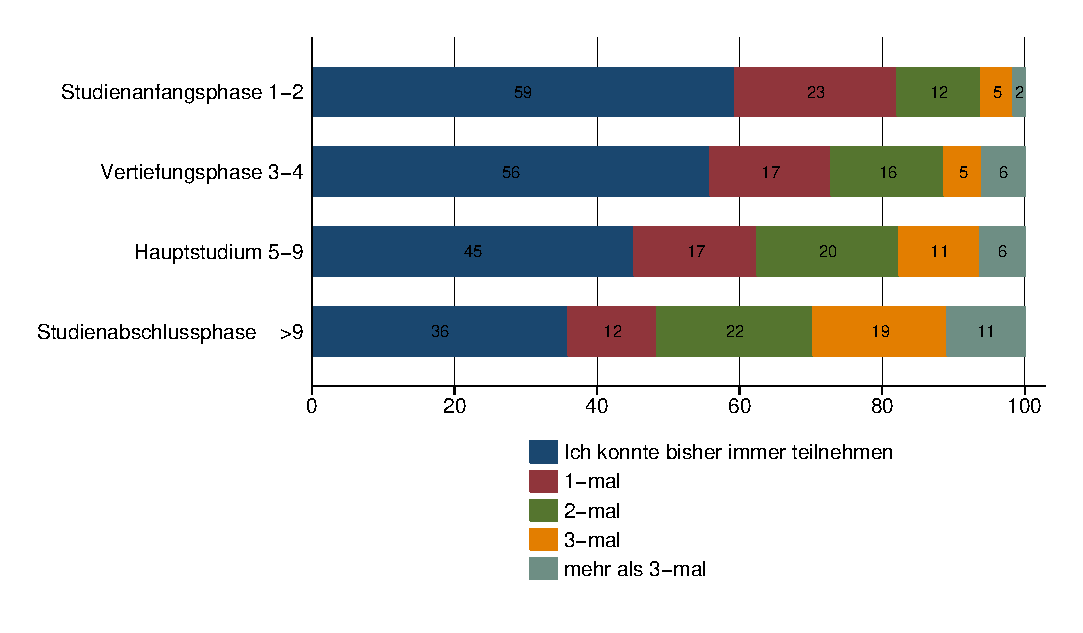
\includegraphics[RemoveGraphicsExtensions={.pdf,PDF}]{image}|
% \end{quote}
%
% \subsection{\plainTeX}
%
% \LaTeX's graphics packages can also be used with \plainTeX.
% The necessary basic \LaTeX\ macros are defined in
% \xfile{miniltx.tex}. This package \xpackage{grfext} also
% relies on it. Example:
%\begin{quote}
%\begin{verbatim}
%\input miniltx.tex\relax
%\def\Gin@driver{pdftex.def}
%\input graphicx.sty\relax
%\input grfext.sty\relax
%\resetatcatcode
%\end{verbatim}
%\end{quote}
%
% \StopEventually{
% }
%
% \section{Implementation}
%
%    \begin{macrocode}
%<*package>
%    \end{macrocode}
%
% \subsection{Relead check and identification}
%    Reload check, especially if the package is not used with \LaTeX.
%    \begin{macrocode}
\begingroup\catcode61\catcode48\catcode32=10\relax%
  \catcode13=5 % ^^M
  \endlinechar=13 %
  \catcode35=6 % #
  \catcode39=12 % '
  \catcode44=12 % ,
  \catcode45=12 % -
  \catcode46=12 % .
  \catcode58=12 % :
  \catcode64=11 % @
  \catcode123=1 % {
  \catcode125=2 % }
  \expandafter\let\expandafter\x\csname ver@grfext.sty\endcsname
  \ifx\x\relax % plain-TeX, first loading
  \else
    \def\empty{}%
    \ifx\x\empty % LaTeX, first loading,
      % variable is initialized, but \ProvidesPackage not yet seen
    \else
      \expandafter\ifx\csname PackageInfo\endcsname\relax
        \def\x#1#2{%
          \immediate\write-1{Package #1 Info: #2.}%
        }%
      \else
        \def\x#1#2{\PackageInfo{#1}{#2, stopped}}%
      \fi
      \x{grfext}{The package is already loaded}%
      \aftergroup\endinput
    \fi
  \fi
\endgroup%
%    \end{macrocode}
%    Package identification:
%    \begin{macrocode}
\begingroup\catcode61\catcode48\catcode32=10\relax%
  \catcode13=5 % ^^M
  \endlinechar=13 %
  \catcode35=6 % #
  \catcode39=12 % '
  \catcode40=12 % (
  \catcode41=12 % )
  \catcode44=12 % ,
  \catcode45=12 % -
  \catcode46=12 % .
  \catcode47=12 % /
  \catcode58=12 % :
  \catcode64=11 % @
  \catcode91=12 % [
  \catcode93=12 % ]
  \catcode123=1 % {
  \catcode125=2 % }
  \expandafter\ifx\csname ProvidesPackage\endcsname\relax
    \def\x#1#2#3[#4]{\endgroup
      \immediate\write-1{Package: #3 #4}%
      \xdef#1{#4}%
    }%
  \else
    \def\x#1#2[#3]{\endgroup
      #2[{#3}]%
      \ifx#1\@undefined
        \xdef#1{#3}%
      \fi
      \ifx#1\relax
        \xdef#1{#3}%
      \fi
    }%
  \fi
\expandafter\x\csname ver@grfext.sty\endcsname
\ProvidesPackage{grfext}%
  [2019/12/03 v1.3 Manage graphics extensions (HO)]%
%    \end{macrocode}
%
% \subsection{Catcodes}
%
%    \begin{macrocode}
\begingroup\catcode61\catcode48\catcode32=10\relax%
  \catcode13=5 % ^^M
  \endlinechar=13 %
  \catcode123=1 % {
  \catcode125=2 % }
  \catcode64=11 % @
  \def\x{\endgroup
    \expandafter\edef\csname grfext@AtEnd\endcsname{%
      \endlinechar=\the\endlinechar\relax
      \catcode13=\the\catcode13\relax
      \catcode32=\the\catcode32\relax
      \catcode35=\the\catcode35\relax
      \catcode61=\the\catcode61\relax
      \catcode64=\the\catcode64\relax
      \catcode123=\the\catcode123\relax
      \catcode125=\the\catcode125\relax
    }%
  }%
\x\catcode61\catcode48\catcode32=10\relax%
\catcode13=5 % ^^M
\endlinechar=13 %
\catcode35=6 % #
\catcode64=11 % @
\catcode123=1 % {
\catcode125=2 % }
\def\TMP@EnsureCode#1#2{%
  \edef\grfext@AtEnd{%
    \grfext@AtEnd
    \catcode#1=\the\catcode#1\relax
  }%
  \catcode#1=#2\relax
}
\TMP@EnsureCode{42}{12}% *
\TMP@EnsureCode{44}{12}% ,
\TMP@EnsureCode{47}{12}% /
\TMP@EnsureCode{58}{12}% :
\TMP@EnsureCode{60}{12}% <
\TMP@EnsureCode{62}{12}% >
\TMP@EnsureCode{91}{12}% [
\TMP@EnsureCode{93}{12}% ]
\edef\grfext@AtEnd{\grfext@AtEnd\noexpand\endinput}
%    \end{macrocode}
%
% \subsection{\plainTeX}
%
%    \begin{macro}{\@expandtwoargs}
%    Requirement is \xfile{miniltx.tex}, but we need also
%    \LaTeX's \cs{@expandtwoargs}.
%    \begin{macrocode}
\@ifundefined{@expandtwoargs}{%
  \def\@expandtwoargs#1#2#3{%
    \edef\reserved@a{\noexpand#1{#2}{#3}}%
    \reserved@a
  }%
}{}
%    \end{macrocode}
%    \end{macro}
%
% \subsection{Add}
%
%    \begin{macro}{\AppendGraphicsExtensions}
%    \begin{macrocode}
\newcommand*{\AppendGraphicsExtensions}{%
  \@ifundefined{Gin@extensions}{%
    \let\Gin@extensions\@empty
  }{}%
  \@ifstar{\grfext@Append\grfext@Check}{\grfext@Append\grfext@@Add}%
}%
%    \end{macrocode}
%    \end{macro}
%    \begin{macro}{\grfext@Append}
%    \begin{macrocode}
\def\grfext@Append#1#2{%
  \let\grfext@Print\@gobble
  \edef\grfext@next{%
    \noexpand\grfext@Add\noexpand#1{%
      \zap@space#2 \@empty
    }{\noexpand\Gin@extensions,}{}%
  }%
  \grfext@next
  \let\grfext@Print\grfext@@Print
  \grfext@Print\AppendGraphicsExtensions
}
%    \end{macrocode}
%    \end{macro}
%
%    \begin{macro}{\PrependGraphicsExtensions}
%    \begin{macrocode}
\newcommand*{\PrependGraphicsExtensions}{%
  \@ifundefined{Gin@extensions}{%
    \let\Gin@extensions\@empty
  }{}%
  \@ifstar{\grfext@Prepend\grfext@Check}{\grfext@Prepend\grfext@@Add}%
}%
%    \end{macrocode}
%    \end{macro}
%    \begin{macro}{\grfext@Prepend}
%    \begin{macrocode}
\def\grfext@Prepend#1#2{%
  \let\grfext@Print\@gobble
  \edef\grfext@next{%
    \noexpand\grfext@Add\noexpand#1{%
      \zap@space#2 \@empty
    }{}{,\noexpand\Gin@extensions}%
  }%
  \grfext@next
  \let\grfext@Print\grfext@@Print
  \grfext@Print\PrependGraphicsExtensions
}
%    \end{macrocode}
%    \end{macro}
%
%    \begin{macro}{\grfext@Add}
%    \begin{macrocode}
\def\grfext@Add#1#2{%
  #1{#2}%
}
%    \end{macrocode}
%    \end{macro}
%    \begin{macro}{\grfext@@Add}
%    \begin{macrocode}
\def\grfext@@Add#1#2#3{%
  \RemoveGraphicsExtensions{#1}%
  \ifx\Gin@extensions\@empty
    \def\Gin@extensions{#1}%
  \else
    \edef\Gin@extensions{#2#1#3}%
  \fi
}
%    \end{macrocode}
%    \end{macro}
%
% \subsection{Check}
%
%    \begin{macro}{\grfext@Check}
%    \begin{macrocode}
\def\grfext@Check#1{%
  \let\grfext@tmp\@empty
  \@for\grfext@ext:=#1\do{%
    \@ifundefined{Gin@rule@\grfext@ext}{%
    }{%
      \ifx\grfext@tmp\@empty
        \let\grfext@tmp\grfext@ext
      \else
        \edef\grfext@tmp{\grfext@tmp,\grfext@ext}%
      \fi
    }%
  }%
  \ifx\grfext@tmp\@empty
    \def\grfext@next##1##2{}%
  \else
    \edef\grfext@next{%
      \noexpand\grfext@@Add{\grfext@tmp}%
    }%
  \fi
  \grfext@next
}
%    \end{macrocode}
%    \end{macro}
%
% \subsection{Remove}
%
%    \begin{macro}{\RemoveGraphicsExtensions}
%    \begin{macrocode}
\newcommand*{\RemoveGraphicsExtensions}[1]{%
  \@ifundefined{Gin@extensions}{%
    \def\Gin@extensions{}%
  }{%
    \edef\grfext@tmp{\zap@space#1 \@empty}%
    \@for\grfext@ext:=\grfext@tmp\do{%
      \def\grfext@next{%
        \let\grfext@tmp\Gin@extensions
        \@expandtwoargs
        \@removeelement\grfext@ext\Gin@extensions\Gin@extensions
        \ifx\grfext@tmp\Gin@extensions
          \let\grfext@next\relax
        \fi
        \grfext@next
      }%
      \grfext@next
    }%
  }%
  \grfext@Print\RemoveGraphicsExtensions
}
%    \end{macrocode}
%    \end{macro}
%
% \subsection{Print}
%
%    \begin{macrocode}
\RequirePackage{infwarerr}[2007/09/09]
%    \end{macrocode}
%
%    \begin{macro}{\PrintGraphicsExtensions}
%    \begin{macrocode}
\def\PrintGraphicsExtensions{%
  \grfext@Print\PrintGraphicsExtensions
}
%    \end{macrocode}
%    \end{macro}
%    \begin{macro}{\grfext@Print}
%    \begin{macrocode}
\def\grfext@Print#1{%
  \@PackageInfo{grfext}{%
    Graphics extension search list:\MessageBreak
    \@ifundefined{Gin@extensions}{%
      <unavailable>%
    }{%
      [\Gin@extensions]%
    }\MessageBreak
    \string#1%
  }%
}
%    \end{macrocode}
%    \end{macro}
%    \begin{macro}{\grfext@@Print}
%    \begin{macrocode}
\let\grfext@@Print\grfext@Print
%    \end{macrocode}
%    \end{macro}
%
% \subsection{Defining options for package \xpackage{graphicx}}
%
%    \begin{macrocode}
\RequirePackage{kvdefinekeys}[2010/03/01]
\kv@define@key{Gin}{AppendGraphicsExtensions}{%
  \AppendGraphicsExtensions{#1}%
}
\kv@define@key{Gin}{AppendGraphicsExtensions*}{%
  \AppendGraphicsExtensions*{#1}%
}
\kv@define@key{Gin}{PrependGraphicsExtensions}{%
  \PrependGraphicsExtensions{#1}%
}
\kv@define@key{Gin}{PrependGraphicsExtensions*}{%
  \PrependGraphicsExtensions*{#1}%
}
\kv@define@key{Gin}{RemoveGraphicsExtensions}{%
  \RemoveGraphicsExtensions{#1}%
}
\kv@define@key{Gin}{PrintGraphicsExtensions}[]{%
  \PrintGraphicsExtensions
}
%    \end{macrocode}
%
%    \begin{macrocode}
\grfext@AtEnd%
%</package>
%    \end{macrocode}
% \section{Installation}
%
% \subsection{Download}
%
% \paragraph{Package.} This package is available on
% CTAN\footnote{\CTANpkg{grfext}}:
% \begin{description}
% \item[\CTAN{macros/latex/contrib/grfext/grfext.dtx}] The source file.
% \item[\CTAN{macros/latex/contrib/grfext/grfext.pdf}] Documentation.
% \end{description}
%
%
% \paragraph{Bundle.} All the packages of the bundle `grfext'
% are also available in a TDS compliant ZIP archive. There
% the packages are already unpacked and the documentation files
% are generated. The files and directories obey the TDS standard.
% \begin{description}
% \item[\CTANinstall{install/macros/latex/contrib/grfext.tds.zip}]
% \end{description}
% \emph{TDS} refers to the standard ``A Directory Structure
% for \TeX\ Files'' (\CTANpkg{tds}). Directories
% with \xfile{texmf} in their name are usually organized this way.
%
% \subsection{Bundle installation}
%
% \paragraph{Unpacking.} Unpack the \xfile{grfext.tds.zip} in the
% TDS tree (also known as \xfile{texmf} tree) of your choice.
% Example (linux):
% \begin{quote}
%   |unzip grfext.tds.zip -d ~/texmf|
% \end{quote}
%
% \subsection{Package installation}
%
% \paragraph{Unpacking.} The \xfile{.dtx} file is a self-extracting
% \docstrip\ archive. The files are extracted by running the
% \xfile{.dtx} through \plainTeX:
% \begin{quote}
%   \verb|tex grfext.dtx|
% \end{quote}
%
% \paragraph{TDS.} Now the different files must be moved into
% the different directories in your installation TDS tree
% (also known as \xfile{texmf} tree):
% \begin{quote}
% \def\t{^^A
% \begin{tabular}{@{}>{\ttfamily}l@{ $\rightarrow$ }>{\ttfamily}l@{}}
%   grfext.sty & tex/latex/grfext/grfext.sty\\
%   grfext.pdf & doc/latex/grfext/grfext.pdf\\
%   grfext.dtx & source/latex/grfext/grfext.dtx\\
% \end{tabular}^^A
% }^^A
% \sbox0{\t}^^A
% \ifdim\wd0>\linewidth
%   \begingroup
%     \advance\linewidth by\leftmargin
%     \advance\linewidth by\rightmargin
%   \edef\x{\endgroup
%     \def\noexpand\lw{\the\linewidth}^^A
%   }\x
%   \def\lwbox{^^A
%     \leavevmode
%     \hbox to \linewidth{^^A
%       \kern-\leftmargin\relax
%       \hss
%       \usebox0
%       \hss
%       \kern-\rightmargin\relax
%     }^^A
%   }^^A
%   \ifdim\wd0>\lw
%     \sbox0{\small\t}^^A
%     \ifdim\wd0>\linewidth
%       \ifdim\wd0>\lw
%         \sbox0{\footnotesize\t}^^A
%         \ifdim\wd0>\linewidth
%           \ifdim\wd0>\lw
%             \sbox0{\scriptsize\t}^^A
%             \ifdim\wd0>\linewidth
%               \ifdim\wd0>\lw
%                 \sbox0{\tiny\t}^^A
%                 \ifdim\wd0>\linewidth
%                   \lwbox
%                 \else
%                   \usebox0
%                 \fi
%               \else
%                 \lwbox
%               \fi
%             \else
%               \usebox0
%             \fi
%           \else
%             \lwbox
%           \fi
%         \else
%           \usebox0
%         \fi
%       \else
%         \lwbox
%       \fi
%     \else
%       \usebox0
%     \fi
%   \else
%     \lwbox
%   \fi
% \else
%   \usebox0
% \fi
% \end{quote}
% If you have a \xfile{docstrip.cfg} that configures and enables \docstrip's
% TDS installing feature, then some files can already be in the right
% place, see the documentation of \docstrip.
%
% \subsection{Refresh file name databases}
%
% If your \TeX~distribution
% (\TeX\,Live, \mikTeX, \dots) relies on file name databases, you must refresh
% these. For example, \TeX\,Live\ users run \verb|texhash| or
% \verb|mktexlsr|.
%
% \subsection{Some details for the interested}
%
% \paragraph{Unpacking with \LaTeX.}
% The \xfile{.dtx} chooses its action depending on the format:
% \begin{description}
% \item[\plainTeX:] Run \docstrip\ and extract the files.
% \item[\LaTeX:] Generate the documentation.
% \end{description}
% If you insist on using \LaTeX\ for \docstrip\ (really,
% \docstrip\ does not need \LaTeX), then inform the autodetect routine
% about your intention:
% \begin{quote}
%   \verb|latex \let\install=y\input{grfext.dtx}|
% \end{quote}
% Do not forget to quote the argument according to the demands
% of your shell.
%
% \paragraph{Generating the documentation.}
% You can use both the \xfile{.dtx} or the \xfile{.drv} to generate
% the documentation. The process can be configured by the
% configuration file \xfile{ltxdoc.cfg}. For instance, put this
% line into this file, if you want to have A4 as paper format:
% \begin{quote}
%   \verb|\PassOptionsToClass{a4paper}{article}|
% \end{quote}
% An example follows how to generate the
% documentation with pdf\LaTeX:
% \begin{quote}
%\begin{verbatim}
%pdflatex grfext.dtx
%makeindex -s gind.ist grfext.idx
%pdflatex grfext.dtx
%makeindex -s gind.ist grfext.idx
%pdflatex grfext.dtx
%\end{verbatim}
% \end{quote}
%
% \begin{thebibliography}{9}
%
% \bibitem{graphics}
%   David Carlisle, Sebastian Rahtz: \textit{The \xpackage{graphics} package};
%   2006/02/20 v1.0o;
%   \CTAN{macros/latex/required/graphics/graphics.dtx}.
%
% \end{thebibliography}
%
% \begin{History}
%   \begin{Version}{2007/09/30 v1.0}
%   \item
%     First public version.
%   \end{Version}
%   \begin{Version}{2010/08/19 v1.1}
%   \item
%     User macros are also made available as keyval options for
%     package \xpackage{graphicx}.
%   \end{Version}
%   \begin{Version}{2016/05/16 v1.2}
%   \item
%     Documentation updates.
%   \end{Version}
%   \begin{Version}{2019/12/03 v1.3}
%   \item
%     Documentation updates.
%   \end{Version}
% \end{History}
%
% \PrintIndex
%
% \Finale
\endinput

%        (quote the arguments according to the demands of your shell)
%
% Documentation:
%    (a) If grfext.drv is present:
%           latex grfext.drv
%    (b) Without grfext.drv:
%           latex grfext.dtx; ...
%    The class ltxdoc loads the configuration file ltxdoc.cfg
%    if available. Here you can specify further options, e.g.
%    use A4 as paper format:
%       \PassOptionsToClass{a4paper}{article}
%
%    Programm calls to get the documentation (example):
%       pdflatex grfext.dtx
%       makeindex -s gind.ist grfext.idx
%       pdflatex grfext.dtx
%       makeindex -s gind.ist grfext.idx
%       pdflatex grfext.dtx
%
% Installation:
%    TDS:tex/latex/grfext/grfext.sty
%    TDS:doc/latex/grfext/grfext.pdf
%    TDS:source/latex/grfext/grfext.dtx
%
%<*ignore>
\begingroup
  \catcode123=1 %
  \catcode125=2 %
  \def\x{LaTeX2e}%
\expandafter\endgroup
\ifcase 0\ifx\install y1\fi\expandafter
         \ifx\csname processbatchFile\endcsname\relax\else1\fi
         \ifx\fmtname\x\else 1\fi\relax
\else\csname fi\endcsname
%</ignore>
%<*install>
\input docstrip.tex
\Msg{************************************************************************}
\Msg{* Installation}
\Msg{* Package: grfext 2019/12/03 v1.3 Manage graphics extensions (HO)}
\Msg{************************************************************************}

\keepsilent
\askforoverwritefalse

\let\MetaPrefix\relax
\preamble

This is a generated file.

Project: grfext
Version: 2019/12/03 v1.3

Copyright (C)
   2007, 2010 Heiko Oberdiek
   2016-2019 Oberdiek Package Support Group

This work may be distributed and/or modified under the
conditions of the LaTeX Project Public License, either
version 1.3c of this license or (at your option) any later
version. This version of this license is in
   https://www.latex-project.org/lppl/lppl-1-3c.txt
and the latest version of this license is in
   https://www.latex-project.org/lppl.txt
and version 1.3 or later is part of all distributions of
LaTeX version 2005/12/01 or later.

This work has the LPPL maintenance status "maintained".

The Current Maintainers of this work are
Heiko Oberdiek and the Oberdiek Package Support Group
https://github.com/ho-tex/grfext/issues


This work consists of the main source file grfext.dtx
and the derived files
   grfext.sty, grfext.pdf, grfext.ins, grfext.drv.

\endpreamble
\let\MetaPrefix\DoubleperCent

\generate{%
  \file{grfext.ins}{\from{grfext.dtx}{install}}%
  \file{grfext.drv}{\from{grfext.dtx}{driver}}%
  \usedir{tex/latex/grfext}%
  \file{grfext.sty}{\from{grfext.dtx}{package}}%
%  \usedir{doc/latex/grfext/test}%
%  \file{grfext-test1.tex}{\from{grfext.dtx}{test1}}%
%  \file{grfext-test2.tex}{\from{grfext.dtx}{test2}}%
}

\catcode32=13\relax% active space
\let =\space%
\Msg{************************************************************************}
\Msg{*}
\Msg{* To finish the installation you have to move the following}
\Msg{* file into a directory searched by TeX:}
\Msg{*}
\Msg{*     grfext.sty}
\Msg{*}
\Msg{* To produce the documentation run the file `grfext.drv'}
\Msg{* through LaTeX.}
\Msg{*}
\Msg{* Happy TeXing!}
\Msg{*}
\Msg{************************************************************************}

\endbatchfile
%</install>
%<*ignore>
\fi
%</ignore>
%<*driver>
\NeedsTeXFormat{LaTeX2e}
\ProvidesFile{grfext.drv}%
  [2019/12/03 v1.3 Manage graphics extensions (HO)]%
\documentclass{ltxdoc}
\usepackage{holtxdoc}[2011/11/22]
\begin{document}
  \DocInput{grfext.dtx}%
\end{document}
%</driver>
% \fi
%
%
%
% \GetFileInfo{grfext.drv}
%
% \title{The \xpackage{grfext} package}
% \date{2019/12/03 v1.3}
% \author{Heiko Oberdiek\thanks
% {Please report any issues at \url{https://github.com/ho-tex/grfext/issues}}}
%
% \maketitle
%
% \begin{abstract}
% This package provides macros for adding and reordering
% graphics extensions of package \xpackage{graphics}.
% \end{abstract}
%
% \tableofcontents
%
% \section{Documentation}
%
% \subsection{Introduction}
%
% If you are not familiar with \LaTeX's graphics bundle, please
% read its documentation \xfile{grffile} \cite{graphics}.
% The bundle contains two packages for graphics inclusion:
% \xpackage{graphics} and \xpackage{graphicx}. The first one
% is loaded by the second one that adds a key value interface.
%
% Graphics files are included in both cases by macro
% \cs{includegraphics}. The file name extension can be omitted.
% Then the graphics package goes through a list of known
% extensions until it finds the graphics file. This extension list
% is set by \cs{DeclareGraphicsExtensions}. The previous contents
% of the list is overwritten.
%
% \subsection{User interface}
%
% This package \xpackage{grfext} provides macros that adds entries
% to the list or remove them. The list may be empty or even
% undefined before. It is always defined afterwards, but can
% be empty (especially after removing entries).
%
% \begin{declcs}{AppendGraphicsExtensions} * \M{ext-list}\\
%   \cs{PrependGraphicsExtensions} * \M{ext-list}
% \end{declcs}
% The argument \meta{ext-list} is a comma separated list whose
% entries are file name extensions including the dot.
% But first the entries are removed from
% \xpackage{graphics}' extension list to avoid multiple
% occurences of the same extension.
%
% Then macro \cs{AppendGraphicsExtensions} adds the entries
% after the end of \xpackage{graphics}' list, whereas
% macro \cs{PrependGraphicsExtensions} puts them in front
% of the list.
% The order matters if a graphics file is available in
% different acceptable formats. Then the first extension
% wins.
%
% The star version of these commands only adds an extensions,
% if a specific graphics rule exists for that extension.
%
% \begin{declcs}{RemoveGraphicsExtensions} \M{ext-list}
% \end{declcs}
% All occurences of file extensions in \meta{ext-list} are
% removed from \xpackage{graphics}' extension list.
%
% \subsection{Package loading}
%
% The package does not define any options. It is loaded
% as usual in \LaTeX, e.g.:
% \begin{quote}
%   |\usepackage{grfext}|
% \end{quote}
%
% \begin{declcs}{PrintGraphicsExtensions}
% \end{declcs}
% Macro \cs{PrintGraphicsExtensions} writes the current
% graphics extensions list in the \xfile{.log} file.
% The macros described before do this automatically
% after their operation.
%
% \subsection{Option support for package \xpackage{graphicx}}
%
% Package \xpackage{graphicx} uses the interface of package
% \xpackage{keyval} in order to specify options for
% \cs{includegraphics}. The options can also be set using
% \begin{quote}
%   |\setkeys{Gin}{|\meta{options}|}|
% \end{quote}
% The four user macros with the two star forms are available
% as options in family |Gin| as well:
% \begin{quote}
%   |AppendGraphicsExtensions={|\meta{ext-list}|}|\\
%   |AppendGraphicsExtensions*={|\meta{ext-list}|}|\\
%   |PrependGraphicsExtensions={|\meta{ext-list}|}|\\
%   |PrependGraphicsExtensions*{|\meta{ext-list}|}|\\
%   |RemoveGraphicsExtensions={|\meta{ext-list}|}|\\
%   |PrintGraphicsExtensions|
% \end{quote}
% This makes it easier to locally change the extension list
% for an included graphics, e.g.:
% \begin{quote}
%   |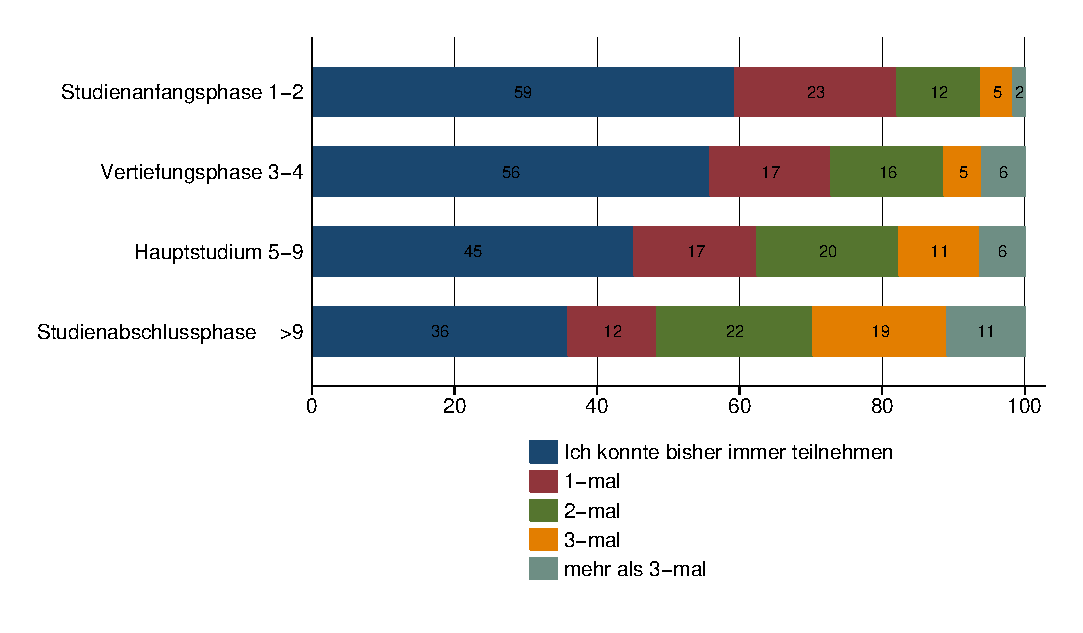
\includegraphics[RemoveGraphicsExtensions={.pdf,PDF}]{image}|
% \end{quote}
%
% \subsection{\plainTeX}
%
% \LaTeX's graphics packages can also be used with \plainTeX.
% The necessary basic \LaTeX\ macros are defined in
% \xfile{miniltx.tex}. This package \xpackage{grfext} also
% relies on it. Example:
%\begin{quote}
%\begin{verbatim}
%\input miniltx.tex\relax
%\def\Gin@driver{pdftex.def}
%\input graphicx.sty\relax
%\input grfext.sty\relax
%\resetatcatcode
%\end{verbatim}
%\end{quote}
%
% \StopEventually{
% }
%
% \section{Implementation}
%
%    \begin{macrocode}
%<*package>
%    \end{macrocode}
%
% \subsection{Relead check and identification}
%    Reload check, especially if the package is not used with \LaTeX.
%    \begin{macrocode}
\begingroup\catcode61\catcode48\catcode32=10\relax%
  \catcode13=5 % ^^M
  \endlinechar=13 %
  \catcode35=6 % #
  \catcode39=12 % '
  \catcode44=12 % ,
  \catcode45=12 % -
  \catcode46=12 % .
  \catcode58=12 % :
  \catcode64=11 % @
  \catcode123=1 % {
  \catcode125=2 % }
  \expandafter\let\expandafter\x\csname ver@grfext.sty\endcsname
  \ifx\x\relax % plain-TeX, first loading
  \else
    \def\empty{}%
    \ifx\x\empty % LaTeX, first loading,
      % variable is initialized, but \ProvidesPackage not yet seen
    \else
      \expandafter\ifx\csname PackageInfo\endcsname\relax
        \def\x#1#2{%
          \immediate\write-1{Package #1 Info: #2.}%
        }%
      \else
        \def\x#1#2{\PackageInfo{#1}{#2, stopped}}%
      \fi
      \x{grfext}{The package is already loaded}%
      \aftergroup\endinput
    \fi
  \fi
\endgroup%
%    \end{macrocode}
%    Package identification:
%    \begin{macrocode}
\begingroup\catcode61\catcode48\catcode32=10\relax%
  \catcode13=5 % ^^M
  \endlinechar=13 %
  \catcode35=6 % #
  \catcode39=12 % '
  \catcode40=12 % (
  \catcode41=12 % )
  \catcode44=12 % ,
  \catcode45=12 % -
  \catcode46=12 % .
  \catcode47=12 % /
  \catcode58=12 % :
  \catcode64=11 % @
  \catcode91=12 % [
  \catcode93=12 % ]
  \catcode123=1 % {
  \catcode125=2 % }
  \expandafter\ifx\csname ProvidesPackage\endcsname\relax
    \def\x#1#2#3[#4]{\endgroup
      \immediate\write-1{Package: #3 #4}%
      \xdef#1{#4}%
    }%
  \else
    \def\x#1#2[#3]{\endgroup
      #2[{#3}]%
      \ifx#1\@undefined
        \xdef#1{#3}%
      \fi
      \ifx#1\relax
        \xdef#1{#3}%
      \fi
    }%
  \fi
\expandafter\x\csname ver@grfext.sty\endcsname
\ProvidesPackage{grfext}%
  [2019/12/03 v1.3 Manage graphics extensions (HO)]%
%    \end{macrocode}
%
% \subsection{Catcodes}
%
%    \begin{macrocode}
\begingroup\catcode61\catcode48\catcode32=10\relax%
  \catcode13=5 % ^^M
  \endlinechar=13 %
  \catcode123=1 % {
  \catcode125=2 % }
  \catcode64=11 % @
  \def\x{\endgroup
    \expandafter\edef\csname grfext@AtEnd\endcsname{%
      \endlinechar=\the\endlinechar\relax
      \catcode13=\the\catcode13\relax
      \catcode32=\the\catcode32\relax
      \catcode35=\the\catcode35\relax
      \catcode61=\the\catcode61\relax
      \catcode64=\the\catcode64\relax
      \catcode123=\the\catcode123\relax
      \catcode125=\the\catcode125\relax
    }%
  }%
\x\catcode61\catcode48\catcode32=10\relax%
\catcode13=5 % ^^M
\endlinechar=13 %
\catcode35=6 % #
\catcode64=11 % @
\catcode123=1 % {
\catcode125=2 % }
\def\TMP@EnsureCode#1#2{%
  \edef\grfext@AtEnd{%
    \grfext@AtEnd
    \catcode#1=\the\catcode#1\relax
  }%
  \catcode#1=#2\relax
}
\TMP@EnsureCode{42}{12}% *
\TMP@EnsureCode{44}{12}% ,
\TMP@EnsureCode{47}{12}% /
\TMP@EnsureCode{58}{12}% :
\TMP@EnsureCode{60}{12}% <
\TMP@EnsureCode{62}{12}% >
\TMP@EnsureCode{91}{12}% [
\TMP@EnsureCode{93}{12}% ]
\edef\grfext@AtEnd{\grfext@AtEnd\noexpand\endinput}
%    \end{macrocode}
%
% \subsection{\plainTeX}
%
%    \begin{macro}{\@expandtwoargs}
%    Requirement is \xfile{miniltx.tex}, but we need also
%    \LaTeX's \cs{@expandtwoargs}.
%    \begin{macrocode}
\@ifundefined{@expandtwoargs}{%
  \def\@expandtwoargs#1#2#3{%
    \edef\reserved@a{\noexpand#1{#2}{#3}}%
    \reserved@a
  }%
}{}
%    \end{macrocode}
%    \end{macro}
%
% \subsection{Add}
%
%    \begin{macro}{\AppendGraphicsExtensions}
%    \begin{macrocode}
\newcommand*{\AppendGraphicsExtensions}{%
  \@ifundefined{Gin@extensions}{%
    \let\Gin@extensions\@empty
  }{}%
  \@ifstar{\grfext@Append\grfext@Check}{\grfext@Append\grfext@@Add}%
}%
%    \end{macrocode}
%    \end{macro}
%    \begin{macro}{\grfext@Append}
%    \begin{macrocode}
\def\grfext@Append#1#2{%
  \let\grfext@Print\@gobble
  \edef\grfext@next{%
    \noexpand\grfext@Add\noexpand#1{%
      \zap@space#2 \@empty
    }{\noexpand\Gin@extensions,}{}%
  }%
  \grfext@next
  \let\grfext@Print\grfext@@Print
  \grfext@Print\AppendGraphicsExtensions
}
%    \end{macrocode}
%    \end{macro}
%
%    \begin{macro}{\PrependGraphicsExtensions}
%    \begin{macrocode}
\newcommand*{\PrependGraphicsExtensions}{%
  \@ifundefined{Gin@extensions}{%
    \let\Gin@extensions\@empty
  }{}%
  \@ifstar{\grfext@Prepend\grfext@Check}{\grfext@Prepend\grfext@@Add}%
}%
%    \end{macrocode}
%    \end{macro}
%    \begin{macro}{\grfext@Prepend}
%    \begin{macrocode}
\def\grfext@Prepend#1#2{%
  \let\grfext@Print\@gobble
  \edef\grfext@next{%
    \noexpand\grfext@Add\noexpand#1{%
      \zap@space#2 \@empty
    }{}{,\noexpand\Gin@extensions}%
  }%
  \grfext@next
  \let\grfext@Print\grfext@@Print
  \grfext@Print\PrependGraphicsExtensions
}
%    \end{macrocode}
%    \end{macro}
%
%    \begin{macro}{\grfext@Add}
%    \begin{macrocode}
\def\grfext@Add#1#2{%
  #1{#2}%
}
%    \end{macrocode}
%    \end{macro}
%    \begin{macro}{\grfext@@Add}
%    \begin{macrocode}
\def\grfext@@Add#1#2#3{%
  \RemoveGraphicsExtensions{#1}%
  \ifx\Gin@extensions\@empty
    \def\Gin@extensions{#1}%
  \else
    \edef\Gin@extensions{#2#1#3}%
  \fi
}
%    \end{macrocode}
%    \end{macro}
%
% \subsection{Check}
%
%    \begin{macro}{\grfext@Check}
%    \begin{macrocode}
\def\grfext@Check#1{%
  \let\grfext@tmp\@empty
  \@for\grfext@ext:=#1\do{%
    \@ifundefined{Gin@rule@\grfext@ext}{%
    }{%
      \ifx\grfext@tmp\@empty
        \let\grfext@tmp\grfext@ext
      \else
        \edef\grfext@tmp{\grfext@tmp,\grfext@ext}%
      \fi
    }%
  }%
  \ifx\grfext@tmp\@empty
    \def\grfext@next##1##2{}%
  \else
    \edef\grfext@next{%
      \noexpand\grfext@@Add{\grfext@tmp}%
    }%
  \fi
  \grfext@next
}
%    \end{macrocode}
%    \end{macro}
%
% \subsection{Remove}
%
%    \begin{macro}{\RemoveGraphicsExtensions}
%    \begin{macrocode}
\newcommand*{\RemoveGraphicsExtensions}[1]{%
  \@ifundefined{Gin@extensions}{%
    \def\Gin@extensions{}%
  }{%
    \edef\grfext@tmp{\zap@space#1 \@empty}%
    \@for\grfext@ext:=\grfext@tmp\do{%
      \def\grfext@next{%
        \let\grfext@tmp\Gin@extensions
        \@expandtwoargs
        \@removeelement\grfext@ext\Gin@extensions\Gin@extensions
        \ifx\grfext@tmp\Gin@extensions
          \let\grfext@next\relax
        \fi
        \grfext@next
      }%
      \grfext@next
    }%
  }%
  \grfext@Print\RemoveGraphicsExtensions
}
%    \end{macrocode}
%    \end{macro}
%
% \subsection{Print}
%
%    \begin{macrocode}
\RequirePackage{infwarerr}[2007/09/09]
%    \end{macrocode}
%
%    \begin{macro}{\PrintGraphicsExtensions}
%    \begin{macrocode}
\def\PrintGraphicsExtensions{%
  \grfext@Print\PrintGraphicsExtensions
}
%    \end{macrocode}
%    \end{macro}
%    \begin{macro}{\grfext@Print}
%    \begin{macrocode}
\def\grfext@Print#1{%
  \@PackageInfo{grfext}{%
    Graphics extension search list:\MessageBreak
    \@ifundefined{Gin@extensions}{%
      <unavailable>%
    }{%
      [\Gin@extensions]%
    }\MessageBreak
    \string#1%
  }%
}
%    \end{macrocode}
%    \end{macro}
%    \begin{macro}{\grfext@@Print}
%    \begin{macrocode}
\let\grfext@@Print\grfext@Print
%    \end{macrocode}
%    \end{macro}
%
% \subsection{Defining options for package \xpackage{graphicx}}
%
%    \begin{macrocode}
\RequirePackage{kvdefinekeys}[2010/03/01]
\kv@define@key{Gin}{AppendGraphicsExtensions}{%
  \AppendGraphicsExtensions{#1}%
}
\kv@define@key{Gin}{AppendGraphicsExtensions*}{%
  \AppendGraphicsExtensions*{#1}%
}
\kv@define@key{Gin}{PrependGraphicsExtensions}{%
  \PrependGraphicsExtensions{#1}%
}
\kv@define@key{Gin}{PrependGraphicsExtensions*}{%
  \PrependGraphicsExtensions*{#1}%
}
\kv@define@key{Gin}{RemoveGraphicsExtensions}{%
  \RemoveGraphicsExtensions{#1}%
}
\kv@define@key{Gin}{PrintGraphicsExtensions}[]{%
  \PrintGraphicsExtensions
}
%    \end{macrocode}
%
%    \begin{macrocode}
\grfext@AtEnd%
%</package>
%    \end{macrocode}
% \section{Installation}
%
% \subsection{Download}
%
% \paragraph{Package.} This package is available on
% CTAN\footnote{\CTANpkg{grfext}}:
% \begin{description}
% \item[\CTAN{macros/latex/contrib/grfext/grfext.dtx}] The source file.
% \item[\CTAN{macros/latex/contrib/grfext/grfext.pdf}] Documentation.
% \end{description}
%
%
% \paragraph{Bundle.} All the packages of the bundle `grfext'
% are also available in a TDS compliant ZIP archive. There
% the packages are already unpacked and the documentation files
% are generated. The files and directories obey the TDS standard.
% \begin{description}
% \item[\CTANinstall{install/macros/latex/contrib/grfext.tds.zip}]
% \end{description}
% \emph{TDS} refers to the standard ``A Directory Structure
% for \TeX\ Files'' (\CTANpkg{tds}). Directories
% with \xfile{texmf} in their name are usually organized this way.
%
% \subsection{Bundle installation}
%
% \paragraph{Unpacking.} Unpack the \xfile{grfext.tds.zip} in the
% TDS tree (also known as \xfile{texmf} tree) of your choice.
% Example (linux):
% \begin{quote}
%   |unzip grfext.tds.zip -d ~/texmf|
% \end{quote}
%
% \subsection{Package installation}
%
% \paragraph{Unpacking.} The \xfile{.dtx} file is a self-extracting
% \docstrip\ archive. The files are extracted by running the
% \xfile{.dtx} through \plainTeX:
% \begin{quote}
%   \verb|tex grfext.dtx|
% \end{quote}
%
% \paragraph{TDS.} Now the different files must be moved into
% the different directories in your installation TDS tree
% (also known as \xfile{texmf} tree):
% \begin{quote}
% \def\t{^^A
% \begin{tabular}{@{}>{\ttfamily}l@{ $\rightarrow$ }>{\ttfamily}l@{}}
%   grfext.sty & tex/latex/grfext/grfext.sty\\
%   grfext.pdf & doc/latex/grfext/grfext.pdf\\
%   grfext.dtx & source/latex/grfext/grfext.dtx\\
% \end{tabular}^^A
% }^^A
% \sbox0{\t}^^A
% \ifdim\wd0>\linewidth
%   \begingroup
%     \advance\linewidth by\leftmargin
%     \advance\linewidth by\rightmargin
%   \edef\x{\endgroup
%     \def\noexpand\lw{\the\linewidth}^^A
%   }\x
%   \def\lwbox{^^A
%     \leavevmode
%     \hbox to \linewidth{^^A
%       \kern-\leftmargin\relax
%       \hss
%       \usebox0
%       \hss
%       \kern-\rightmargin\relax
%     }^^A
%   }^^A
%   \ifdim\wd0>\lw
%     \sbox0{\small\t}^^A
%     \ifdim\wd0>\linewidth
%       \ifdim\wd0>\lw
%         \sbox0{\footnotesize\t}^^A
%         \ifdim\wd0>\linewidth
%           \ifdim\wd0>\lw
%             \sbox0{\scriptsize\t}^^A
%             \ifdim\wd0>\linewidth
%               \ifdim\wd0>\lw
%                 \sbox0{\tiny\t}^^A
%                 \ifdim\wd0>\linewidth
%                   \lwbox
%                 \else
%                   \usebox0
%                 \fi
%               \else
%                 \lwbox
%               \fi
%             \else
%               \usebox0
%             \fi
%           \else
%             \lwbox
%           \fi
%         \else
%           \usebox0
%         \fi
%       \else
%         \lwbox
%       \fi
%     \else
%       \usebox0
%     \fi
%   \else
%     \lwbox
%   \fi
% \else
%   \usebox0
% \fi
% \end{quote}
% If you have a \xfile{docstrip.cfg} that configures and enables \docstrip's
% TDS installing feature, then some files can already be in the right
% place, see the documentation of \docstrip.
%
% \subsection{Refresh file name databases}
%
% If your \TeX~distribution
% (\TeX\,Live, \mikTeX, \dots) relies on file name databases, you must refresh
% these. For example, \TeX\,Live\ users run \verb|texhash| or
% \verb|mktexlsr|.
%
% \subsection{Some details for the interested}
%
% \paragraph{Unpacking with \LaTeX.}
% The \xfile{.dtx} chooses its action depending on the format:
% \begin{description}
% \item[\plainTeX:] Run \docstrip\ and extract the files.
% \item[\LaTeX:] Generate the documentation.
% \end{description}
% If you insist on using \LaTeX\ for \docstrip\ (really,
% \docstrip\ does not need \LaTeX), then inform the autodetect routine
% about your intention:
% \begin{quote}
%   \verb|latex \let\install=y% \iffalse meta-comment
%
% File: grfext.dtx
% Version: 2019/12/03 v1.3
% Info: Manage graphics extensions
%
% Copyright (C)
%    2007, 2010 Heiko Oberdiek
%    2016-2019 Oberdiek Package Support Group
%    https://github.com/ho-tex/grfext/issues
%
% This work may be distributed and/or modified under the
% conditions of the LaTeX Project Public License, either
% version 1.3c of this license or (at your option) any later
% version. This version of this license is in
%    https://www.latex-project.org/lppl/lppl-1-3c.txt
% and the latest version of this license is in
%    https://www.latex-project.org/lppl.txt
% and version 1.3 or later is part of all distributions of
% LaTeX version 2005/12/01 or later.
%
% This work has the LPPL maintenance status "maintained".
%
% The Current Maintainers of this work are
% Heiko Oberdiek and the Oberdiek Package Support Group
% https://github.com/ho-tex/grfext/issues
%
% This work consists of the main source file grfext.dtx
% and the derived files
%    grfext.sty, grfext.pdf, grfext.ins, grfext.drv,
%
% Distribution:
%    CTAN:macros/latex/contrib/grfext/grfext.dtx
%    CTAN:macros/latex/contrib/grfext/grfext.pdf
%
% Unpacking:
%    (a) If grfext.ins is present:
%           tex grfext.ins
%    (b) Without grfext.ins:
%           tex grfext.dtx
%    (c) If you insist on using LaTeX
%           latex \let\install=y\input{grfext.dtx}
%        (quote the arguments according to the demands of your shell)
%
% Documentation:
%    (a) If grfext.drv is present:
%           latex grfext.drv
%    (b) Without grfext.drv:
%           latex grfext.dtx; ...
%    The class ltxdoc loads the configuration file ltxdoc.cfg
%    if available. Here you can specify further options, e.g.
%    use A4 as paper format:
%       \PassOptionsToClass{a4paper}{article}
%
%    Programm calls to get the documentation (example):
%       pdflatex grfext.dtx
%       makeindex -s gind.ist grfext.idx
%       pdflatex grfext.dtx
%       makeindex -s gind.ist grfext.idx
%       pdflatex grfext.dtx
%
% Installation:
%    TDS:tex/latex/grfext/grfext.sty
%    TDS:doc/latex/grfext/grfext.pdf
%    TDS:source/latex/grfext/grfext.dtx
%
%<*ignore>
\begingroup
  \catcode123=1 %
  \catcode125=2 %
  \def\x{LaTeX2e}%
\expandafter\endgroup
\ifcase 0\ifx\install y1\fi\expandafter
         \ifx\csname processbatchFile\endcsname\relax\else1\fi
         \ifx\fmtname\x\else 1\fi\relax
\else\csname fi\endcsname
%</ignore>
%<*install>
\input docstrip.tex
\Msg{************************************************************************}
\Msg{* Installation}
\Msg{* Package: grfext 2019/12/03 v1.3 Manage graphics extensions (HO)}
\Msg{************************************************************************}

\keepsilent
\askforoverwritefalse

\let\MetaPrefix\relax
\preamble

This is a generated file.

Project: grfext
Version: 2019/12/03 v1.3

Copyright (C)
   2007, 2010 Heiko Oberdiek
   2016-2019 Oberdiek Package Support Group

This work may be distributed and/or modified under the
conditions of the LaTeX Project Public License, either
version 1.3c of this license or (at your option) any later
version. This version of this license is in
   https://www.latex-project.org/lppl/lppl-1-3c.txt
and the latest version of this license is in
   https://www.latex-project.org/lppl.txt
and version 1.3 or later is part of all distributions of
LaTeX version 2005/12/01 or later.

This work has the LPPL maintenance status "maintained".

The Current Maintainers of this work are
Heiko Oberdiek and the Oberdiek Package Support Group
https://github.com/ho-tex/grfext/issues


This work consists of the main source file grfext.dtx
and the derived files
   grfext.sty, grfext.pdf, grfext.ins, grfext.drv.

\endpreamble
\let\MetaPrefix\DoubleperCent

\generate{%
  \file{grfext.ins}{\from{grfext.dtx}{install}}%
  \file{grfext.drv}{\from{grfext.dtx}{driver}}%
  \usedir{tex/latex/grfext}%
  \file{grfext.sty}{\from{grfext.dtx}{package}}%
%  \usedir{doc/latex/grfext/test}%
%  \file{grfext-test1.tex}{\from{grfext.dtx}{test1}}%
%  \file{grfext-test2.tex}{\from{grfext.dtx}{test2}}%
}

\catcode32=13\relax% active space
\let =\space%
\Msg{************************************************************************}
\Msg{*}
\Msg{* To finish the installation you have to move the following}
\Msg{* file into a directory searched by TeX:}
\Msg{*}
\Msg{*     grfext.sty}
\Msg{*}
\Msg{* To produce the documentation run the file `grfext.drv'}
\Msg{* through LaTeX.}
\Msg{*}
\Msg{* Happy TeXing!}
\Msg{*}
\Msg{************************************************************************}

\endbatchfile
%</install>
%<*ignore>
\fi
%</ignore>
%<*driver>
\NeedsTeXFormat{LaTeX2e}
\ProvidesFile{grfext.drv}%
  [2019/12/03 v1.3 Manage graphics extensions (HO)]%
\documentclass{ltxdoc}
\usepackage{holtxdoc}[2011/11/22]
\begin{document}
  \DocInput{grfext.dtx}%
\end{document}
%</driver>
% \fi
%
%
%
% \GetFileInfo{grfext.drv}
%
% \title{The \xpackage{grfext} package}
% \date{2019/12/03 v1.3}
% \author{Heiko Oberdiek\thanks
% {Please report any issues at \url{https://github.com/ho-tex/grfext/issues}}}
%
% \maketitle
%
% \begin{abstract}
% This package provides macros for adding and reordering
% graphics extensions of package \xpackage{graphics}.
% \end{abstract}
%
% \tableofcontents
%
% \section{Documentation}
%
% \subsection{Introduction}
%
% If you are not familiar with \LaTeX's graphics bundle, please
% read its documentation \xfile{grffile} \cite{graphics}.
% The bundle contains two packages for graphics inclusion:
% \xpackage{graphics} and \xpackage{graphicx}. The first one
% is loaded by the second one that adds a key value interface.
%
% Graphics files are included in both cases by macro
% \cs{includegraphics}. The file name extension can be omitted.
% Then the graphics package goes through a list of known
% extensions until it finds the graphics file. This extension list
% is set by \cs{DeclareGraphicsExtensions}. The previous contents
% of the list is overwritten.
%
% \subsection{User interface}
%
% This package \xpackage{grfext} provides macros that adds entries
% to the list or remove them. The list may be empty or even
% undefined before. It is always defined afterwards, but can
% be empty (especially after removing entries).
%
% \begin{declcs}{AppendGraphicsExtensions} * \M{ext-list}\\
%   \cs{PrependGraphicsExtensions} * \M{ext-list}
% \end{declcs}
% The argument \meta{ext-list} is a comma separated list whose
% entries are file name extensions including the dot.
% But first the entries are removed from
% \xpackage{graphics}' extension list to avoid multiple
% occurences of the same extension.
%
% Then macro \cs{AppendGraphicsExtensions} adds the entries
% after the end of \xpackage{graphics}' list, whereas
% macro \cs{PrependGraphicsExtensions} puts them in front
% of the list.
% The order matters if a graphics file is available in
% different acceptable formats. Then the first extension
% wins.
%
% The star version of these commands only adds an extensions,
% if a specific graphics rule exists for that extension.
%
% \begin{declcs}{RemoveGraphicsExtensions} \M{ext-list}
% \end{declcs}
% All occurences of file extensions in \meta{ext-list} are
% removed from \xpackage{graphics}' extension list.
%
% \subsection{Package loading}
%
% The package does not define any options. It is loaded
% as usual in \LaTeX, e.g.:
% \begin{quote}
%   |\usepackage{grfext}|
% \end{quote}
%
% \begin{declcs}{PrintGraphicsExtensions}
% \end{declcs}
% Macro \cs{PrintGraphicsExtensions} writes the current
% graphics extensions list in the \xfile{.log} file.
% The macros described before do this automatically
% after their operation.
%
% \subsection{Option support for package \xpackage{graphicx}}
%
% Package \xpackage{graphicx} uses the interface of package
% \xpackage{keyval} in order to specify options for
% \cs{includegraphics}. The options can also be set using
% \begin{quote}
%   |\setkeys{Gin}{|\meta{options}|}|
% \end{quote}
% The four user macros with the two star forms are available
% as options in family |Gin| as well:
% \begin{quote}
%   |AppendGraphicsExtensions={|\meta{ext-list}|}|\\
%   |AppendGraphicsExtensions*={|\meta{ext-list}|}|\\
%   |PrependGraphicsExtensions={|\meta{ext-list}|}|\\
%   |PrependGraphicsExtensions*{|\meta{ext-list}|}|\\
%   |RemoveGraphicsExtensions={|\meta{ext-list}|}|\\
%   |PrintGraphicsExtensions|
% \end{quote}
% This makes it easier to locally change the extension list
% for an included graphics, e.g.:
% \begin{quote}
%   |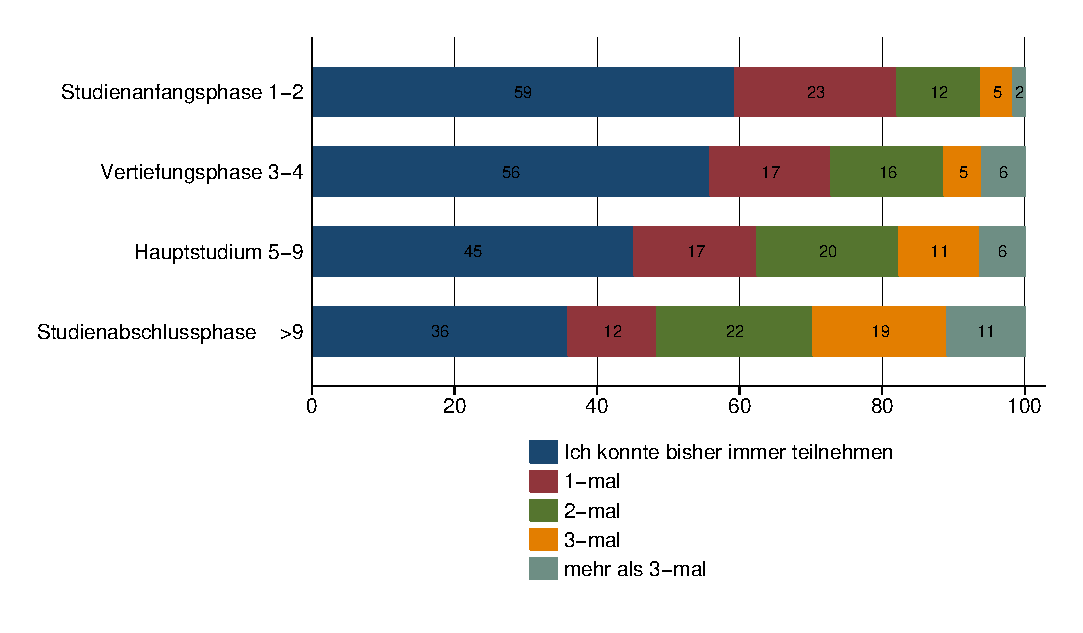
\includegraphics[RemoveGraphicsExtensions={.pdf,PDF}]{image}|
% \end{quote}
%
% \subsection{\plainTeX}
%
% \LaTeX's graphics packages can also be used with \plainTeX.
% The necessary basic \LaTeX\ macros are defined in
% \xfile{miniltx.tex}. This package \xpackage{grfext} also
% relies on it. Example:
%\begin{quote}
%\begin{verbatim}
%\input miniltx.tex\relax
%\def\Gin@driver{pdftex.def}
%\input graphicx.sty\relax
%\input grfext.sty\relax
%\resetatcatcode
%\end{verbatim}
%\end{quote}
%
% \StopEventually{
% }
%
% \section{Implementation}
%
%    \begin{macrocode}
%<*package>
%    \end{macrocode}
%
% \subsection{Relead check and identification}
%    Reload check, especially if the package is not used with \LaTeX.
%    \begin{macrocode}
\begingroup\catcode61\catcode48\catcode32=10\relax%
  \catcode13=5 % ^^M
  \endlinechar=13 %
  \catcode35=6 % #
  \catcode39=12 % '
  \catcode44=12 % ,
  \catcode45=12 % -
  \catcode46=12 % .
  \catcode58=12 % :
  \catcode64=11 % @
  \catcode123=1 % {
  \catcode125=2 % }
  \expandafter\let\expandafter\x\csname ver@grfext.sty\endcsname
  \ifx\x\relax % plain-TeX, first loading
  \else
    \def\empty{}%
    \ifx\x\empty % LaTeX, first loading,
      % variable is initialized, but \ProvidesPackage not yet seen
    \else
      \expandafter\ifx\csname PackageInfo\endcsname\relax
        \def\x#1#2{%
          \immediate\write-1{Package #1 Info: #2.}%
        }%
      \else
        \def\x#1#2{\PackageInfo{#1}{#2, stopped}}%
      \fi
      \x{grfext}{The package is already loaded}%
      \aftergroup\endinput
    \fi
  \fi
\endgroup%
%    \end{macrocode}
%    Package identification:
%    \begin{macrocode}
\begingroup\catcode61\catcode48\catcode32=10\relax%
  \catcode13=5 % ^^M
  \endlinechar=13 %
  \catcode35=6 % #
  \catcode39=12 % '
  \catcode40=12 % (
  \catcode41=12 % )
  \catcode44=12 % ,
  \catcode45=12 % -
  \catcode46=12 % .
  \catcode47=12 % /
  \catcode58=12 % :
  \catcode64=11 % @
  \catcode91=12 % [
  \catcode93=12 % ]
  \catcode123=1 % {
  \catcode125=2 % }
  \expandafter\ifx\csname ProvidesPackage\endcsname\relax
    \def\x#1#2#3[#4]{\endgroup
      \immediate\write-1{Package: #3 #4}%
      \xdef#1{#4}%
    }%
  \else
    \def\x#1#2[#3]{\endgroup
      #2[{#3}]%
      \ifx#1\@undefined
        \xdef#1{#3}%
      \fi
      \ifx#1\relax
        \xdef#1{#3}%
      \fi
    }%
  \fi
\expandafter\x\csname ver@grfext.sty\endcsname
\ProvidesPackage{grfext}%
  [2019/12/03 v1.3 Manage graphics extensions (HO)]%
%    \end{macrocode}
%
% \subsection{Catcodes}
%
%    \begin{macrocode}
\begingroup\catcode61\catcode48\catcode32=10\relax%
  \catcode13=5 % ^^M
  \endlinechar=13 %
  \catcode123=1 % {
  \catcode125=2 % }
  \catcode64=11 % @
  \def\x{\endgroup
    \expandafter\edef\csname grfext@AtEnd\endcsname{%
      \endlinechar=\the\endlinechar\relax
      \catcode13=\the\catcode13\relax
      \catcode32=\the\catcode32\relax
      \catcode35=\the\catcode35\relax
      \catcode61=\the\catcode61\relax
      \catcode64=\the\catcode64\relax
      \catcode123=\the\catcode123\relax
      \catcode125=\the\catcode125\relax
    }%
  }%
\x\catcode61\catcode48\catcode32=10\relax%
\catcode13=5 % ^^M
\endlinechar=13 %
\catcode35=6 % #
\catcode64=11 % @
\catcode123=1 % {
\catcode125=2 % }
\def\TMP@EnsureCode#1#2{%
  \edef\grfext@AtEnd{%
    \grfext@AtEnd
    \catcode#1=\the\catcode#1\relax
  }%
  \catcode#1=#2\relax
}
\TMP@EnsureCode{42}{12}% *
\TMP@EnsureCode{44}{12}% ,
\TMP@EnsureCode{47}{12}% /
\TMP@EnsureCode{58}{12}% :
\TMP@EnsureCode{60}{12}% <
\TMP@EnsureCode{62}{12}% >
\TMP@EnsureCode{91}{12}% [
\TMP@EnsureCode{93}{12}% ]
\edef\grfext@AtEnd{\grfext@AtEnd\noexpand\endinput}
%    \end{macrocode}
%
% \subsection{\plainTeX}
%
%    \begin{macro}{\@expandtwoargs}
%    Requirement is \xfile{miniltx.tex}, but we need also
%    \LaTeX's \cs{@expandtwoargs}.
%    \begin{macrocode}
\@ifundefined{@expandtwoargs}{%
  \def\@expandtwoargs#1#2#3{%
    \edef\reserved@a{\noexpand#1{#2}{#3}}%
    \reserved@a
  }%
}{}
%    \end{macrocode}
%    \end{macro}
%
% \subsection{Add}
%
%    \begin{macro}{\AppendGraphicsExtensions}
%    \begin{macrocode}
\newcommand*{\AppendGraphicsExtensions}{%
  \@ifundefined{Gin@extensions}{%
    \let\Gin@extensions\@empty
  }{}%
  \@ifstar{\grfext@Append\grfext@Check}{\grfext@Append\grfext@@Add}%
}%
%    \end{macrocode}
%    \end{macro}
%    \begin{macro}{\grfext@Append}
%    \begin{macrocode}
\def\grfext@Append#1#2{%
  \let\grfext@Print\@gobble
  \edef\grfext@next{%
    \noexpand\grfext@Add\noexpand#1{%
      \zap@space#2 \@empty
    }{\noexpand\Gin@extensions,}{}%
  }%
  \grfext@next
  \let\grfext@Print\grfext@@Print
  \grfext@Print\AppendGraphicsExtensions
}
%    \end{macrocode}
%    \end{macro}
%
%    \begin{macro}{\PrependGraphicsExtensions}
%    \begin{macrocode}
\newcommand*{\PrependGraphicsExtensions}{%
  \@ifundefined{Gin@extensions}{%
    \let\Gin@extensions\@empty
  }{}%
  \@ifstar{\grfext@Prepend\grfext@Check}{\grfext@Prepend\grfext@@Add}%
}%
%    \end{macrocode}
%    \end{macro}
%    \begin{macro}{\grfext@Prepend}
%    \begin{macrocode}
\def\grfext@Prepend#1#2{%
  \let\grfext@Print\@gobble
  \edef\grfext@next{%
    \noexpand\grfext@Add\noexpand#1{%
      \zap@space#2 \@empty
    }{}{,\noexpand\Gin@extensions}%
  }%
  \grfext@next
  \let\grfext@Print\grfext@@Print
  \grfext@Print\PrependGraphicsExtensions
}
%    \end{macrocode}
%    \end{macro}
%
%    \begin{macro}{\grfext@Add}
%    \begin{macrocode}
\def\grfext@Add#1#2{%
  #1{#2}%
}
%    \end{macrocode}
%    \end{macro}
%    \begin{macro}{\grfext@@Add}
%    \begin{macrocode}
\def\grfext@@Add#1#2#3{%
  \RemoveGraphicsExtensions{#1}%
  \ifx\Gin@extensions\@empty
    \def\Gin@extensions{#1}%
  \else
    \edef\Gin@extensions{#2#1#3}%
  \fi
}
%    \end{macrocode}
%    \end{macro}
%
% \subsection{Check}
%
%    \begin{macro}{\grfext@Check}
%    \begin{macrocode}
\def\grfext@Check#1{%
  \let\grfext@tmp\@empty
  \@for\grfext@ext:=#1\do{%
    \@ifundefined{Gin@rule@\grfext@ext}{%
    }{%
      \ifx\grfext@tmp\@empty
        \let\grfext@tmp\grfext@ext
      \else
        \edef\grfext@tmp{\grfext@tmp,\grfext@ext}%
      \fi
    }%
  }%
  \ifx\grfext@tmp\@empty
    \def\grfext@next##1##2{}%
  \else
    \edef\grfext@next{%
      \noexpand\grfext@@Add{\grfext@tmp}%
    }%
  \fi
  \grfext@next
}
%    \end{macrocode}
%    \end{macro}
%
% \subsection{Remove}
%
%    \begin{macro}{\RemoveGraphicsExtensions}
%    \begin{macrocode}
\newcommand*{\RemoveGraphicsExtensions}[1]{%
  \@ifundefined{Gin@extensions}{%
    \def\Gin@extensions{}%
  }{%
    \edef\grfext@tmp{\zap@space#1 \@empty}%
    \@for\grfext@ext:=\grfext@tmp\do{%
      \def\grfext@next{%
        \let\grfext@tmp\Gin@extensions
        \@expandtwoargs
        \@removeelement\grfext@ext\Gin@extensions\Gin@extensions
        \ifx\grfext@tmp\Gin@extensions
          \let\grfext@next\relax
        \fi
        \grfext@next
      }%
      \grfext@next
    }%
  }%
  \grfext@Print\RemoveGraphicsExtensions
}
%    \end{macrocode}
%    \end{macro}
%
% \subsection{Print}
%
%    \begin{macrocode}
\RequirePackage{infwarerr}[2007/09/09]
%    \end{macrocode}
%
%    \begin{macro}{\PrintGraphicsExtensions}
%    \begin{macrocode}
\def\PrintGraphicsExtensions{%
  \grfext@Print\PrintGraphicsExtensions
}
%    \end{macrocode}
%    \end{macro}
%    \begin{macro}{\grfext@Print}
%    \begin{macrocode}
\def\grfext@Print#1{%
  \@PackageInfo{grfext}{%
    Graphics extension search list:\MessageBreak
    \@ifundefined{Gin@extensions}{%
      <unavailable>%
    }{%
      [\Gin@extensions]%
    }\MessageBreak
    \string#1%
  }%
}
%    \end{macrocode}
%    \end{macro}
%    \begin{macro}{\grfext@@Print}
%    \begin{macrocode}
\let\grfext@@Print\grfext@Print
%    \end{macrocode}
%    \end{macro}
%
% \subsection{Defining options for package \xpackage{graphicx}}
%
%    \begin{macrocode}
\RequirePackage{kvdefinekeys}[2010/03/01]
\kv@define@key{Gin}{AppendGraphicsExtensions}{%
  \AppendGraphicsExtensions{#1}%
}
\kv@define@key{Gin}{AppendGraphicsExtensions*}{%
  \AppendGraphicsExtensions*{#1}%
}
\kv@define@key{Gin}{PrependGraphicsExtensions}{%
  \PrependGraphicsExtensions{#1}%
}
\kv@define@key{Gin}{PrependGraphicsExtensions*}{%
  \PrependGraphicsExtensions*{#1}%
}
\kv@define@key{Gin}{RemoveGraphicsExtensions}{%
  \RemoveGraphicsExtensions{#1}%
}
\kv@define@key{Gin}{PrintGraphicsExtensions}[]{%
  \PrintGraphicsExtensions
}
%    \end{macrocode}
%
%    \begin{macrocode}
\grfext@AtEnd%
%</package>
%    \end{macrocode}
% \section{Installation}
%
% \subsection{Download}
%
% \paragraph{Package.} This package is available on
% CTAN\footnote{\CTANpkg{grfext}}:
% \begin{description}
% \item[\CTAN{macros/latex/contrib/grfext/grfext.dtx}] The source file.
% \item[\CTAN{macros/latex/contrib/grfext/grfext.pdf}] Documentation.
% \end{description}
%
%
% \paragraph{Bundle.} All the packages of the bundle `grfext'
% are also available in a TDS compliant ZIP archive. There
% the packages are already unpacked and the documentation files
% are generated. The files and directories obey the TDS standard.
% \begin{description}
% \item[\CTANinstall{install/macros/latex/contrib/grfext.tds.zip}]
% \end{description}
% \emph{TDS} refers to the standard ``A Directory Structure
% for \TeX\ Files'' (\CTANpkg{tds}). Directories
% with \xfile{texmf} in their name are usually organized this way.
%
% \subsection{Bundle installation}
%
% \paragraph{Unpacking.} Unpack the \xfile{grfext.tds.zip} in the
% TDS tree (also known as \xfile{texmf} tree) of your choice.
% Example (linux):
% \begin{quote}
%   |unzip grfext.tds.zip -d ~/texmf|
% \end{quote}
%
% \subsection{Package installation}
%
% \paragraph{Unpacking.} The \xfile{.dtx} file is a self-extracting
% \docstrip\ archive. The files are extracted by running the
% \xfile{.dtx} through \plainTeX:
% \begin{quote}
%   \verb|tex grfext.dtx|
% \end{quote}
%
% \paragraph{TDS.} Now the different files must be moved into
% the different directories in your installation TDS tree
% (also known as \xfile{texmf} tree):
% \begin{quote}
% \def\t{^^A
% \begin{tabular}{@{}>{\ttfamily}l@{ $\rightarrow$ }>{\ttfamily}l@{}}
%   grfext.sty & tex/latex/grfext/grfext.sty\\
%   grfext.pdf & doc/latex/grfext/grfext.pdf\\
%   grfext.dtx & source/latex/grfext/grfext.dtx\\
% \end{tabular}^^A
% }^^A
% \sbox0{\t}^^A
% \ifdim\wd0>\linewidth
%   \begingroup
%     \advance\linewidth by\leftmargin
%     \advance\linewidth by\rightmargin
%   \edef\x{\endgroup
%     \def\noexpand\lw{\the\linewidth}^^A
%   }\x
%   \def\lwbox{^^A
%     \leavevmode
%     \hbox to \linewidth{^^A
%       \kern-\leftmargin\relax
%       \hss
%       \usebox0
%       \hss
%       \kern-\rightmargin\relax
%     }^^A
%   }^^A
%   \ifdim\wd0>\lw
%     \sbox0{\small\t}^^A
%     \ifdim\wd0>\linewidth
%       \ifdim\wd0>\lw
%         \sbox0{\footnotesize\t}^^A
%         \ifdim\wd0>\linewidth
%           \ifdim\wd0>\lw
%             \sbox0{\scriptsize\t}^^A
%             \ifdim\wd0>\linewidth
%               \ifdim\wd0>\lw
%                 \sbox0{\tiny\t}^^A
%                 \ifdim\wd0>\linewidth
%                   \lwbox
%                 \else
%                   \usebox0
%                 \fi
%               \else
%                 \lwbox
%               \fi
%             \else
%               \usebox0
%             \fi
%           \else
%             \lwbox
%           \fi
%         \else
%           \usebox0
%         \fi
%       \else
%         \lwbox
%       \fi
%     \else
%       \usebox0
%     \fi
%   \else
%     \lwbox
%   \fi
% \else
%   \usebox0
% \fi
% \end{quote}
% If you have a \xfile{docstrip.cfg} that configures and enables \docstrip's
% TDS installing feature, then some files can already be in the right
% place, see the documentation of \docstrip.
%
% \subsection{Refresh file name databases}
%
% If your \TeX~distribution
% (\TeX\,Live, \mikTeX, \dots) relies on file name databases, you must refresh
% these. For example, \TeX\,Live\ users run \verb|texhash| or
% \verb|mktexlsr|.
%
% \subsection{Some details for the interested}
%
% \paragraph{Unpacking with \LaTeX.}
% The \xfile{.dtx} chooses its action depending on the format:
% \begin{description}
% \item[\plainTeX:] Run \docstrip\ and extract the files.
% \item[\LaTeX:] Generate the documentation.
% \end{description}
% If you insist on using \LaTeX\ for \docstrip\ (really,
% \docstrip\ does not need \LaTeX), then inform the autodetect routine
% about your intention:
% \begin{quote}
%   \verb|latex \let\install=y\input{grfext.dtx}|
% \end{quote}
% Do not forget to quote the argument according to the demands
% of your shell.
%
% \paragraph{Generating the documentation.}
% You can use both the \xfile{.dtx} or the \xfile{.drv} to generate
% the documentation. The process can be configured by the
% configuration file \xfile{ltxdoc.cfg}. For instance, put this
% line into this file, if you want to have A4 as paper format:
% \begin{quote}
%   \verb|\PassOptionsToClass{a4paper}{article}|
% \end{quote}
% An example follows how to generate the
% documentation with pdf\LaTeX:
% \begin{quote}
%\begin{verbatim}
%pdflatex grfext.dtx
%makeindex -s gind.ist grfext.idx
%pdflatex grfext.dtx
%makeindex -s gind.ist grfext.idx
%pdflatex grfext.dtx
%\end{verbatim}
% \end{quote}
%
% \begin{thebibliography}{9}
%
% \bibitem{graphics}
%   David Carlisle, Sebastian Rahtz: \textit{The \xpackage{graphics} package};
%   2006/02/20 v1.0o;
%   \CTAN{macros/latex/required/graphics/graphics.dtx}.
%
% \end{thebibliography}
%
% \begin{History}
%   \begin{Version}{2007/09/30 v1.0}
%   \item
%     First public version.
%   \end{Version}
%   \begin{Version}{2010/08/19 v1.1}
%   \item
%     User macros are also made available as keyval options for
%     package \xpackage{graphicx}.
%   \end{Version}
%   \begin{Version}{2016/05/16 v1.2}
%   \item
%     Documentation updates.
%   \end{Version}
%   \begin{Version}{2019/12/03 v1.3}
%   \item
%     Documentation updates.
%   \end{Version}
% \end{History}
%
% \PrintIndex
%
% \Finale
\endinput
|
% \end{quote}
% Do not forget to quote the argument according to the demands
% of your shell.
%
% \paragraph{Generating the documentation.}
% You can use both the \xfile{.dtx} or the \xfile{.drv} to generate
% the documentation. The process can be configured by the
% configuration file \xfile{ltxdoc.cfg}. For instance, put this
% line into this file, if you want to have A4 as paper format:
% \begin{quote}
%   \verb|\PassOptionsToClass{a4paper}{article}|
% \end{quote}
% An example follows how to generate the
% documentation with pdf\LaTeX:
% \begin{quote}
%\begin{verbatim}
%pdflatex grfext.dtx
%makeindex -s gind.ist grfext.idx
%pdflatex grfext.dtx
%makeindex -s gind.ist grfext.idx
%pdflatex grfext.dtx
%\end{verbatim}
% \end{quote}
%
% \begin{thebibliography}{9}
%
% \bibitem{graphics}
%   David Carlisle, Sebastian Rahtz: \textit{The \xpackage{graphics} package};
%   2006/02/20 v1.0o;
%   \CTAN{macros/latex/required/graphics/graphics.dtx}.
%
% \end{thebibliography}
%
% \begin{History}
%   \begin{Version}{2007/09/30 v1.0}
%   \item
%     First public version.
%   \end{Version}
%   \begin{Version}{2010/08/19 v1.1}
%   \item
%     User macros are also made available as keyval options for
%     package \xpackage{graphicx}.
%   \end{Version}
%   \begin{Version}{2016/05/16 v1.2}
%   \item
%     Documentation updates.
%   \end{Version}
%   \begin{Version}{2019/12/03 v1.3}
%   \item
%     Documentation updates.
%   \end{Version}
% \end{History}
%
% \PrintIndex
%
% \Finale
\endinput

%        (quote the arguments according to the demands of your shell)
%
% Documentation:
%    (a) If grfext.drv is present:
%           latex grfext.drv
%    (b) Without grfext.drv:
%           latex grfext.dtx; ...
%    The class ltxdoc loads the configuration file ltxdoc.cfg
%    if available. Here you can specify further options, e.g.
%    use A4 as paper format:
%       \PassOptionsToClass{a4paper}{article}
%
%    Programm calls to get the documentation (example):
%       pdflatex grfext.dtx
%       makeindex -s gind.ist grfext.idx
%       pdflatex grfext.dtx
%       makeindex -s gind.ist grfext.idx
%       pdflatex grfext.dtx
%
% Installation:
%    TDS:tex/latex/grfext/grfext.sty
%    TDS:doc/latex/grfext/grfext.pdf
%    TDS:source/latex/grfext/grfext.dtx
%
%<*ignore>
\begingroup
  \catcode123=1 %
  \catcode125=2 %
  \def\x{LaTeX2e}%
\expandafter\endgroup
\ifcase 0\ifx\install y1\fi\expandafter
         \ifx\csname processbatchFile\endcsname\relax\else1\fi
         \ifx\fmtname\x\else 1\fi\relax
\else\csname fi\endcsname
%</ignore>
%<*install>
\input docstrip.tex
\Msg{************************************************************************}
\Msg{* Installation}
\Msg{* Package: grfext 2019/12/03 v1.3 Manage graphics extensions (HO)}
\Msg{************************************************************************}

\keepsilent
\askforoverwritefalse

\let\MetaPrefix\relax
\preamble

This is a generated file.

Project: grfext
Version: 2019/12/03 v1.3

Copyright (C)
   2007, 2010 Heiko Oberdiek
   2016-2019 Oberdiek Package Support Group

This work may be distributed and/or modified under the
conditions of the LaTeX Project Public License, either
version 1.3c of this license or (at your option) any later
version. This version of this license is in
   https://www.latex-project.org/lppl/lppl-1-3c.txt
and the latest version of this license is in
   https://www.latex-project.org/lppl.txt
and version 1.3 or later is part of all distributions of
LaTeX version 2005/12/01 or later.

This work has the LPPL maintenance status "maintained".

The Current Maintainers of this work are
Heiko Oberdiek and the Oberdiek Package Support Group
https://github.com/ho-tex/grfext/issues


This work consists of the main source file grfext.dtx
and the derived files
   grfext.sty, grfext.pdf, grfext.ins, grfext.drv.

\endpreamble
\let\MetaPrefix\DoubleperCent

\generate{%
  \file{grfext.ins}{\from{grfext.dtx}{install}}%
  \file{grfext.drv}{\from{grfext.dtx}{driver}}%
  \usedir{tex/latex/grfext}%
  \file{grfext.sty}{\from{grfext.dtx}{package}}%
%  \usedir{doc/latex/grfext/test}%
%  \file{grfext-test1.tex}{\from{grfext.dtx}{test1}}%
%  \file{grfext-test2.tex}{\from{grfext.dtx}{test2}}%
}

\catcode32=13\relax% active space
\let =\space%
\Msg{************************************************************************}
\Msg{*}
\Msg{* To finish the installation you have to move the following}
\Msg{* file into a directory searched by TeX:}
\Msg{*}
\Msg{*     grfext.sty}
\Msg{*}
\Msg{* To produce the documentation run the file `grfext.drv'}
\Msg{* through LaTeX.}
\Msg{*}
\Msg{* Happy TeXing!}
\Msg{*}
\Msg{************************************************************************}

\endbatchfile
%</install>
%<*ignore>
\fi
%</ignore>
%<*driver>
\NeedsTeXFormat{LaTeX2e}
\ProvidesFile{grfext.drv}%
  [2019/12/03 v1.3 Manage graphics extensions (HO)]%
\documentclass{ltxdoc}
\usepackage{holtxdoc}[2011/11/22]
\begin{document}
  \DocInput{grfext.dtx}%
\end{document}
%</driver>
% \fi
%
%
%
% \GetFileInfo{grfext.drv}
%
% \title{The \xpackage{grfext} package}
% \date{2019/12/03 v1.3}
% \author{Heiko Oberdiek\thanks
% {Please report any issues at \url{https://github.com/ho-tex/grfext/issues}}}
%
% \maketitle
%
% \begin{abstract}
% This package provides macros for adding and reordering
% graphics extensions of package \xpackage{graphics}.
% \end{abstract}
%
% \tableofcontents
%
% \section{Documentation}
%
% \subsection{Introduction}
%
% If you are not familiar with \LaTeX's graphics bundle, please
% read its documentation \xfile{grffile} \cite{graphics}.
% The bundle contains two packages for graphics inclusion:
% \xpackage{graphics} and \xpackage{graphicx}. The first one
% is loaded by the second one that adds a key value interface.
%
% Graphics files are included in both cases by macro
% \cs{includegraphics}. The file name extension can be omitted.
% Then the graphics package goes through a list of known
% extensions until it finds the graphics file. This extension list
% is set by \cs{DeclareGraphicsExtensions}. The previous contents
% of the list is overwritten.
%
% \subsection{User interface}
%
% This package \xpackage{grfext} provides macros that adds entries
% to the list or remove them. The list may be empty or even
% undefined before. It is always defined afterwards, but can
% be empty (especially after removing entries).
%
% \begin{declcs}{AppendGraphicsExtensions} * \M{ext-list}\\
%   \cs{PrependGraphicsExtensions} * \M{ext-list}
% \end{declcs}
% The argument \meta{ext-list} is a comma separated list whose
% entries are file name extensions including the dot.
% But first the entries are removed from
% \xpackage{graphics}' extension list to avoid multiple
% occurences of the same extension.
%
% Then macro \cs{AppendGraphicsExtensions} adds the entries
% after the end of \xpackage{graphics}' list, whereas
% macro \cs{PrependGraphicsExtensions} puts them in front
% of the list.
% The order matters if a graphics file is available in
% different acceptable formats. Then the first extension
% wins.
%
% The star version of these commands only adds an extensions,
% if a specific graphics rule exists for that extension.
%
% \begin{declcs}{RemoveGraphicsExtensions} \M{ext-list}
% \end{declcs}
% All occurences of file extensions in \meta{ext-list} are
% removed from \xpackage{graphics}' extension list.
%
% \subsection{Package loading}
%
% The package does not define any options. It is loaded
% as usual in \LaTeX, e.g.:
% \begin{quote}
%   |\usepackage{grfext}|
% \end{quote}
%
% \begin{declcs}{PrintGraphicsExtensions}
% \end{declcs}
% Macro \cs{PrintGraphicsExtensions} writes the current
% graphics extensions list in the \xfile{.log} file.
% The macros described before do this automatically
% after their operation.
%
% \subsection{Option support for package \xpackage{graphicx}}
%
% Package \xpackage{graphicx} uses the interface of package
% \xpackage{keyval} in order to specify options for
% \cs{includegraphics}. The options can also be set using
% \begin{quote}
%   |\setkeys{Gin}{|\meta{options}|}|
% \end{quote}
% The four user macros with the two star forms are available
% as options in family |Gin| as well:
% \begin{quote}
%   |AppendGraphicsExtensions={|\meta{ext-list}|}|\\
%   |AppendGraphicsExtensions*={|\meta{ext-list}|}|\\
%   |PrependGraphicsExtensions={|\meta{ext-list}|}|\\
%   |PrependGraphicsExtensions*{|\meta{ext-list}|}|\\
%   |RemoveGraphicsExtensions={|\meta{ext-list}|}|\\
%   |PrintGraphicsExtensions|
% \end{quote}
% This makes it easier to locally change the extension list
% for an included graphics, e.g.:
% \begin{quote}
%   |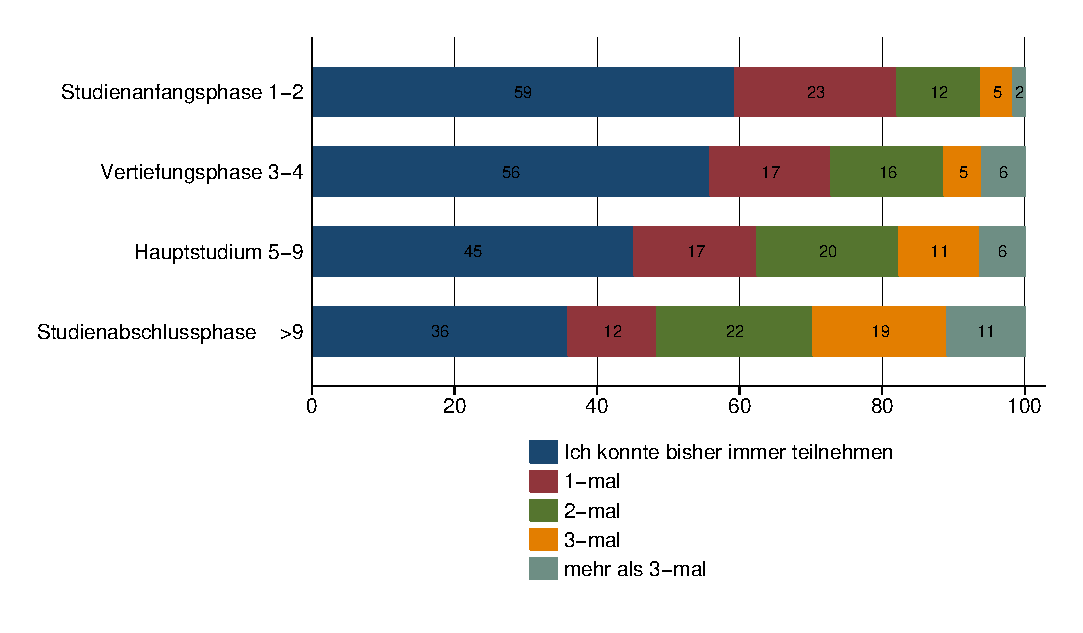
\includegraphics[RemoveGraphicsExtensions={.pdf,PDF}]{image}|
% \end{quote}
%
% \subsection{\plainTeX}
%
% \LaTeX's graphics packages can also be used with \plainTeX.
% The necessary basic \LaTeX\ macros are defined in
% \xfile{miniltx.tex}. This package \xpackage{grfext} also
% relies on it. Example:
%\begin{quote}
%\begin{verbatim}
%\input miniltx.tex\relax
%\def\Gin@driver{pdftex.def}
%\input graphicx.sty\relax
%\input grfext.sty\relax
%\resetatcatcode
%\end{verbatim}
%\end{quote}
%
% \StopEventually{
% }
%
% \section{Implementation}
%
%    \begin{macrocode}
%<*package>
%    \end{macrocode}
%
% \subsection{Relead check and identification}
%    Reload check, especially if the package is not used with \LaTeX.
%    \begin{macrocode}
\begingroup\catcode61\catcode48\catcode32=10\relax%
  \catcode13=5 % ^^M
  \endlinechar=13 %
  \catcode35=6 % #
  \catcode39=12 % '
  \catcode44=12 % ,
  \catcode45=12 % -
  \catcode46=12 % .
  \catcode58=12 % :
  \catcode64=11 % @
  \catcode123=1 % {
  \catcode125=2 % }
  \expandafter\let\expandafter\x\csname ver@grfext.sty\endcsname
  \ifx\x\relax % plain-TeX, first loading
  \else
    \def\empty{}%
    \ifx\x\empty % LaTeX, first loading,
      % variable is initialized, but \ProvidesPackage not yet seen
    \else
      \expandafter\ifx\csname PackageInfo\endcsname\relax
        \def\x#1#2{%
          \immediate\write-1{Package #1 Info: #2.}%
        }%
      \else
        \def\x#1#2{\PackageInfo{#1}{#2, stopped}}%
      \fi
      \x{grfext}{The package is already loaded}%
      \aftergroup\endinput
    \fi
  \fi
\endgroup%
%    \end{macrocode}
%    Package identification:
%    \begin{macrocode}
\begingroup\catcode61\catcode48\catcode32=10\relax%
  \catcode13=5 % ^^M
  \endlinechar=13 %
  \catcode35=6 % #
  \catcode39=12 % '
  \catcode40=12 % (
  \catcode41=12 % )
  \catcode44=12 % ,
  \catcode45=12 % -
  \catcode46=12 % .
  \catcode47=12 % /
  \catcode58=12 % :
  \catcode64=11 % @
  \catcode91=12 % [
  \catcode93=12 % ]
  \catcode123=1 % {
  \catcode125=2 % }
  \expandafter\ifx\csname ProvidesPackage\endcsname\relax
    \def\x#1#2#3[#4]{\endgroup
      \immediate\write-1{Package: #3 #4}%
      \xdef#1{#4}%
    }%
  \else
    \def\x#1#2[#3]{\endgroup
      #2[{#3}]%
      \ifx#1\@undefined
        \xdef#1{#3}%
      \fi
      \ifx#1\relax
        \xdef#1{#3}%
      \fi
    }%
  \fi
\expandafter\x\csname ver@grfext.sty\endcsname
\ProvidesPackage{grfext}%
  [2019/12/03 v1.3 Manage graphics extensions (HO)]%
%    \end{macrocode}
%
% \subsection{Catcodes}
%
%    \begin{macrocode}
\begingroup\catcode61\catcode48\catcode32=10\relax%
  \catcode13=5 % ^^M
  \endlinechar=13 %
  \catcode123=1 % {
  \catcode125=2 % }
  \catcode64=11 % @
  \def\x{\endgroup
    \expandafter\edef\csname grfext@AtEnd\endcsname{%
      \endlinechar=\the\endlinechar\relax
      \catcode13=\the\catcode13\relax
      \catcode32=\the\catcode32\relax
      \catcode35=\the\catcode35\relax
      \catcode61=\the\catcode61\relax
      \catcode64=\the\catcode64\relax
      \catcode123=\the\catcode123\relax
      \catcode125=\the\catcode125\relax
    }%
  }%
\x\catcode61\catcode48\catcode32=10\relax%
\catcode13=5 % ^^M
\endlinechar=13 %
\catcode35=6 % #
\catcode64=11 % @
\catcode123=1 % {
\catcode125=2 % }
\def\TMP@EnsureCode#1#2{%
  \edef\grfext@AtEnd{%
    \grfext@AtEnd
    \catcode#1=\the\catcode#1\relax
  }%
  \catcode#1=#2\relax
}
\TMP@EnsureCode{42}{12}% *
\TMP@EnsureCode{44}{12}% ,
\TMP@EnsureCode{47}{12}% /
\TMP@EnsureCode{58}{12}% :
\TMP@EnsureCode{60}{12}% <
\TMP@EnsureCode{62}{12}% >
\TMP@EnsureCode{91}{12}% [
\TMP@EnsureCode{93}{12}% ]
\edef\grfext@AtEnd{\grfext@AtEnd\noexpand\endinput}
%    \end{macrocode}
%
% \subsection{\plainTeX}
%
%    \begin{macro}{\@expandtwoargs}
%    Requirement is \xfile{miniltx.tex}, but we need also
%    \LaTeX's \cs{@expandtwoargs}.
%    \begin{macrocode}
\@ifundefined{@expandtwoargs}{%
  \def\@expandtwoargs#1#2#3{%
    \edef\reserved@a{\noexpand#1{#2}{#3}}%
    \reserved@a
  }%
}{}
%    \end{macrocode}
%    \end{macro}
%
% \subsection{Add}
%
%    \begin{macro}{\AppendGraphicsExtensions}
%    \begin{macrocode}
\newcommand*{\AppendGraphicsExtensions}{%
  \@ifundefined{Gin@extensions}{%
    \let\Gin@extensions\@empty
  }{}%
  \@ifstar{\grfext@Append\grfext@Check}{\grfext@Append\grfext@@Add}%
}%
%    \end{macrocode}
%    \end{macro}
%    \begin{macro}{\grfext@Append}
%    \begin{macrocode}
\def\grfext@Append#1#2{%
  \let\grfext@Print\@gobble
  \edef\grfext@next{%
    \noexpand\grfext@Add\noexpand#1{%
      \zap@space#2 \@empty
    }{\noexpand\Gin@extensions,}{}%
  }%
  \grfext@next
  \let\grfext@Print\grfext@@Print
  \grfext@Print\AppendGraphicsExtensions
}
%    \end{macrocode}
%    \end{macro}
%
%    \begin{macro}{\PrependGraphicsExtensions}
%    \begin{macrocode}
\newcommand*{\PrependGraphicsExtensions}{%
  \@ifundefined{Gin@extensions}{%
    \let\Gin@extensions\@empty
  }{}%
  \@ifstar{\grfext@Prepend\grfext@Check}{\grfext@Prepend\grfext@@Add}%
}%
%    \end{macrocode}
%    \end{macro}
%    \begin{macro}{\grfext@Prepend}
%    \begin{macrocode}
\def\grfext@Prepend#1#2{%
  \let\grfext@Print\@gobble
  \edef\grfext@next{%
    \noexpand\grfext@Add\noexpand#1{%
      \zap@space#2 \@empty
    }{}{,\noexpand\Gin@extensions}%
  }%
  \grfext@next
  \let\grfext@Print\grfext@@Print
  \grfext@Print\PrependGraphicsExtensions
}
%    \end{macrocode}
%    \end{macro}
%
%    \begin{macro}{\grfext@Add}
%    \begin{macrocode}
\def\grfext@Add#1#2{%
  #1{#2}%
}
%    \end{macrocode}
%    \end{macro}
%    \begin{macro}{\grfext@@Add}
%    \begin{macrocode}
\def\grfext@@Add#1#2#3{%
  \RemoveGraphicsExtensions{#1}%
  \ifx\Gin@extensions\@empty
    \def\Gin@extensions{#1}%
  \else
    \edef\Gin@extensions{#2#1#3}%
  \fi
}
%    \end{macrocode}
%    \end{macro}
%
% \subsection{Check}
%
%    \begin{macro}{\grfext@Check}
%    \begin{macrocode}
\def\grfext@Check#1{%
  \let\grfext@tmp\@empty
  \@for\grfext@ext:=#1\do{%
    \@ifundefined{Gin@rule@\grfext@ext}{%
    }{%
      \ifx\grfext@tmp\@empty
        \let\grfext@tmp\grfext@ext
      \else
        \edef\grfext@tmp{\grfext@tmp,\grfext@ext}%
      \fi
    }%
  }%
  \ifx\grfext@tmp\@empty
    \def\grfext@next##1##2{}%
  \else
    \edef\grfext@next{%
      \noexpand\grfext@@Add{\grfext@tmp}%
    }%
  \fi
  \grfext@next
}
%    \end{macrocode}
%    \end{macro}
%
% \subsection{Remove}
%
%    \begin{macro}{\RemoveGraphicsExtensions}
%    \begin{macrocode}
\newcommand*{\RemoveGraphicsExtensions}[1]{%
  \@ifundefined{Gin@extensions}{%
    \def\Gin@extensions{}%
  }{%
    \edef\grfext@tmp{\zap@space#1 \@empty}%
    \@for\grfext@ext:=\grfext@tmp\do{%
      \def\grfext@next{%
        \let\grfext@tmp\Gin@extensions
        \@expandtwoargs
        \@removeelement\grfext@ext\Gin@extensions\Gin@extensions
        \ifx\grfext@tmp\Gin@extensions
          \let\grfext@next\relax
        \fi
        \grfext@next
      }%
      \grfext@next
    }%
  }%
  \grfext@Print\RemoveGraphicsExtensions
}
%    \end{macrocode}
%    \end{macro}
%
% \subsection{Print}
%
%    \begin{macrocode}
\RequirePackage{infwarerr}[2007/09/09]
%    \end{macrocode}
%
%    \begin{macro}{\PrintGraphicsExtensions}
%    \begin{macrocode}
\def\PrintGraphicsExtensions{%
  \grfext@Print\PrintGraphicsExtensions
}
%    \end{macrocode}
%    \end{macro}
%    \begin{macro}{\grfext@Print}
%    \begin{macrocode}
\def\grfext@Print#1{%
  \@PackageInfo{grfext}{%
    Graphics extension search list:\MessageBreak
    \@ifundefined{Gin@extensions}{%
      <unavailable>%
    }{%
      [\Gin@extensions]%
    }\MessageBreak
    \string#1%
  }%
}
%    \end{macrocode}
%    \end{macro}
%    \begin{macro}{\grfext@@Print}
%    \begin{macrocode}
\let\grfext@@Print\grfext@Print
%    \end{macrocode}
%    \end{macro}
%
% \subsection{Defining options for package \xpackage{graphicx}}
%
%    \begin{macrocode}
\RequirePackage{kvdefinekeys}[2010/03/01]
\kv@define@key{Gin}{AppendGraphicsExtensions}{%
  \AppendGraphicsExtensions{#1}%
}
\kv@define@key{Gin}{AppendGraphicsExtensions*}{%
  \AppendGraphicsExtensions*{#1}%
}
\kv@define@key{Gin}{PrependGraphicsExtensions}{%
  \PrependGraphicsExtensions{#1}%
}
\kv@define@key{Gin}{PrependGraphicsExtensions*}{%
  \PrependGraphicsExtensions*{#1}%
}
\kv@define@key{Gin}{RemoveGraphicsExtensions}{%
  \RemoveGraphicsExtensions{#1}%
}
\kv@define@key{Gin}{PrintGraphicsExtensions}[]{%
  \PrintGraphicsExtensions
}
%    \end{macrocode}
%
%    \begin{macrocode}
\grfext@AtEnd%
%</package>
%    \end{macrocode}
% \section{Installation}
%
% \subsection{Download}
%
% \paragraph{Package.} This package is available on
% CTAN\footnote{\CTANpkg{grfext}}:
% \begin{description}
% \item[\CTAN{macros/latex/contrib/grfext/grfext.dtx}] The source file.
% \item[\CTAN{macros/latex/contrib/grfext/grfext.pdf}] Documentation.
% \end{description}
%
%
% \paragraph{Bundle.} All the packages of the bundle `grfext'
% are also available in a TDS compliant ZIP archive. There
% the packages are already unpacked and the documentation files
% are generated. The files and directories obey the TDS standard.
% \begin{description}
% \item[\CTANinstall{install/macros/latex/contrib/grfext.tds.zip}]
% \end{description}
% \emph{TDS} refers to the standard ``A Directory Structure
% for \TeX\ Files'' (\CTANpkg{tds}). Directories
% with \xfile{texmf} in their name are usually organized this way.
%
% \subsection{Bundle installation}
%
% \paragraph{Unpacking.} Unpack the \xfile{grfext.tds.zip} in the
% TDS tree (also known as \xfile{texmf} tree) of your choice.
% Example (linux):
% \begin{quote}
%   |unzip grfext.tds.zip -d ~/texmf|
% \end{quote}
%
% \subsection{Package installation}
%
% \paragraph{Unpacking.} The \xfile{.dtx} file is a self-extracting
% \docstrip\ archive. The files are extracted by running the
% \xfile{.dtx} through \plainTeX:
% \begin{quote}
%   \verb|tex grfext.dtx|
% \end{quote}
%
% \paragraph{TDS.} Now the different files must be moved into
% the different directories in your installation TDS tree
% (also known as \xfile{texmf} tree):
% \begin{quote}
% \def\t{^^A
% \begin{tabular}{@{}>{\ttfamily}l@{ $\rightarrow$ }>{\ttfamily}l@{}}
%   grfext.sty & tex/latex/grfext/grfext.sty\\
%   grfext.pdf & doc/latex/grfext/grfext.pdf\\
%   grfext.dtx & source/latex/grfext/grfext.dtx\\
% \end{tabular}^^A
% }^^A
% \sbox0{\t}^^A
% \ifdim\wd0>\linewidth
%   \begingroup
%     \advance\linewidth by\leftmargin
%     \advance\linewidth by\rightmargin
%   \edef\x{\endgroup
%     \def\noexpand\lw{\the\linewidth}^^A
%   }\x
%   \def\lwbox{^^A
%     \leavevmode
%     \hbox to \linewidth{^^A
%       \kern-\leftmargin\relax
%       \hss
%       \usebox0
%       \hss
%       \kern-\rightmargin\relax
%     }^^A
%   }^^A
%   \ifdim\wd0>\lw
%     \sbox0{\small\t}^^A
%     \ifdim\wd0>\linewidth
%       \ifdim\wd0>\lw
%         \sbox0{\footnotesize\t}^^A
%         \ifdim\wd0>\linewidth
%           \ifdim\wd0>\lw
%             \sbox0{\scriptsize\t}^^A
%             \ifdim\wd0>\linewidth
%               \ifdim\wd0>\lw
%                 \sbox0{\tiny\t}^^A
%                 \ifdim\wd0>\linewidth
%                   \lwbox
%                 \else
%                   \usebox0
%                 \fi
%               \else
%                 \lwbox
%               \fi
%             \else
%               \usebox0
%             \fi
%           \else
%             \lwbox
%           \fi
%         \else
%           \usebox0
%         \fi
%       \else
%         \lwbox
%       \fi
%     \else
%       \usebox0
%     \fi
%   \else
%     \lwbox
%   \fi
% \else
%   \usebox0
% \fi
% \end{quote}
% If you have a \xfile{docstrip.cfg} that configures and enables \docstrip's
% TDS installing feature, then some files can already be in the right
% place, see the documentation of \docstrip.
%
% \subsection{Refresh file name databases}
%
% If your \TeX~distribution
% (\TeX\,Live, \mikTeX, \dots) relies on file name databases, you must refresh
% these. For example, \TeX\,Live\ users run \verb|texhash| or
% \verb|mktexlsr|.
%
% \subsection{Some details for the interested}
%
% \paragraph{Unpacking with \LaTeX.}
% The \xfile{.dtx} chooses its action depending on the format:
% \begin{description}
% \item[\plainTeX:] Run \docstrip\ and extract the files.
% \item[\LaTeX:] Generate the documentation.
% \end{description}
% If you insist on using \LaTeX\ for \docstrip\ (really,
% \docstrip\ does not need \LaTeX), then inform the autodetect routine
% about your intention:
% \begin{quote}
%   \verb|latex \let\install=y% \iffalse meta-comment
%
% File: grfext.dtx
% Version: 2019/12/03 v1.3
% Info: Manage graphics extensions
%
% Copyright (C)
%    2007, 2010 Heiko Oberdiek
%    2016-2019 Oberdiek Package Support Group
%    https://github.com/ho-tex/grfext/issues
%
% This work may be distributed and/or modified under the
% conditions of the LaTeX Project Public License, either
% version 1.3c of this license or (at your option) any later
% version. This version of this license is in
%    https://www.latex-project.org/lppl/lppl-1-3c.txt
% and the latest version of this license is in
%    https://www.latex-project.org/lppl.txt
% and version 1.3 or later is part of all distributions of
% LaTeX version 2005/12/01 or later.
%
% This work has the LPPL maintenance status "maintained".
%
% The Current Maintainers of this work are
% Heiko Oberdiek and the Oberdiek Package Support Group
% https://github.com/ho-tex/grfext/issues
%
% This work consists of the main source file grfext.dtx
% and the derived files
%    grfext.sty, grfext.pdf, grfext.ins, grfext.drv,
%
% Distribution:
%    CTAN:macros/latex/contrib/grfext/grfext.dtx
%    CTAN:macros/latex/contrib/grfext/grfext.pdf
%
% Unpacking:
%    (a) If grfext.ins is present:
%           tex grfext.ins
%    (b) Without grfext.ins:
%           tex grfext.dtx
%    (c) If you insist on using LaTeX
%           latex \let\install=y% \iffalse meta-comment
%
% File: grfext.dtx
% Version: 2019/12/03 v1.3
% Info: Manage graphics extensions
%
% Copyright (C)
%    2007, 2010 Heiko Oberdiek
%    2016-2019 Oberdiek Package Support Group
%    https://github.com/ho-tex/grfext/issues
%
% This work may be distributed and/or modified under the
% conditions of the LaTeX Project Public License, either
% version 1.3c of this license or (at your option) any later
% version. This version of this license is in
%    https://www.latex-project.org/lppl/lppl-1-3c.txt
% and the latest version of this license is in
%    https://www.latex-project.org/lppl.txt
% and version 1.3 or later is part of all distributions of
% LaTeX version 2005/12/01 or later.
%
% This work has the LPPL maintenance status "maintained".
%
% The Current Maintainers of this work are
% Heiko Oberdiek and the Oberdiek Package Support Group
% https://github.com/ho-tex/grfext/issues
%
% This work consists of the main source file grfext.dtx
% and the derived files
%    grfext.sty, grfext.pdf, grfext.ins, grfext.drv,
%
% Distribution:
%    CTAN:macros/latex/contrib/grfext/grfext.dtx
%    CTAN:macros/latex/contrib/grfext/grfext.pdf
%
% Unpacking:
%    (a) If grfext.ins is present:
%           tex grfext.ins
%    (b) Without grfext.ins:
%           tex grfext.dtx
%    (c) If you insist on using LaTeX
%           latex \let\install=y\input{grfext.dtx}
%        (quote the arguments according to the demands of your shell)
%
% Documentation:
%    (a) If grfext.drv is present:
%           latex grfext.drv
%    (b) Without grfext.drv:
%           latex grfext.dtx; ...
%    The class ltxdoc loads the configuration file ltxdoc.cfg
%    if available. Here you can specify further options, e.g.
%    use A4 as paper format:
%       \PassOptionsToClass{a4paper}{article}
%
%    Programm calls to get the documentation (example):
%       pdflatex grfext.dtx
%       makeindex -s gind.ist grfext.idx
%       pdflatex grfext.dtx
%       makeindex -s gind.ist grfext.idx
%       pdflatex grfext.dtx
%
% Installation:
%    TDS:tex/latex/grfext/grfext.sty
%    TDS:doc/latex/grfext/grfext.pdf
%    TDS:source/latex/grfext/grfext.dtx
%
%<*ignore>
\begingroup
  \catcode123=1 %
  \catcode125=2 %
  \def\x{LaTeX2e}%
\expandafter\endgroup
\ifcase 0\ifx\install y1\fi\expandafter
         \ifx\csname processbatchFile\endcsname\relax\else1\fi
         \ifx\fmtname\x\else 1\fi\relax
\else\csname fi\endcsname
%</ignore>
%<*install>
\input docstrip.tex
\Msg{************************************************************************}
\Msg{* Installation}
\Msg{* Package: grfext 2019/12/03 v1.3 Manage graphics extensions (HO)}
\Msg{************************************************************************}

\keepsilent
\askforoverwritefalse

\let\MetaPrefix\relax
\preamble

This is a generated file.

Project: grfext
Version: 2019/12/03 v1.3

Copyright (C)
   2007, 2010 Heiko Oberdiek
   2016-2019 Oberdiek Package Support Group

This work may be distributed and/or modified under the
conditions of the LaTeX Project Public License, either
version 1.3c of this license or (at your option) any later
version. This version of this license is in
   https://www.latex-project.org/lppl/lppl-1-3c.txt
and the latest version of this license is in
   https://www.latex-project.org/lppl.txt
and version 1.3 or later is part of all distributions of
LaTeX version 2005/12/01 or later.

This work has the LPPL maintenance status "maintained".

The Current Maintainers of this work are
Heiko Oberdiek and the Oberdiek Package Support Group
https://github.com/ho-tex/grfext/issues


This work consists of the main source file grfext.dtx
and the derived files
   grfext.sty, grfext.pdf, grfext.ins, grfext.drv.

\endpreamble
\let\MetaPrefix\DoubleperCent

\generate{%
  \file{grfext.ins}{\from{grfext.dtx}{install}}%
  \file{grfext.drv}{\from{grfext.dtx}{driver}}%
  \usedir{tex/latex/grfext}%
  \file{grfext.sty}{\from{grfext.dtx}{package}}%
%  \usedir{doc/latex/grfext/test}%
%  \file{grfext-test1.tex}{\from{grfext.dtx}{test1}}%
%  \file{grfext-test2.tex}{\from{grfext.dtx}{test2}}%
}

\catcode32=13\relax% active space
\let =\space%
\Msg{************************************************************************}
\Msg{*}
\Msg{* To finish the installation you have to move the following}
\Msg{* file into a directory searched by TeX:}
\Msg{*}
\Msg{*     grfext.sty}
\Msg{*}
\Msg{* To produce the documentation run the file `grfext.drv'}
\Msg{* through LaTeX.}
\Msg{*}
\Msg{* Happy TeXing!}
\Msg{*}
\Msg{************************************************************************}

\endbatchfile
%</install>
%<*ignore>
\fi
%</ignore>
%<*driver>
\NeedsTeXFormat{LaTeX2e}
\ProvidesFile{grfext.drv}%
  [2019/12/03 v1.3 Manage graphics extensions (HO)]%
\documentclass{ltxdoc}
\usepackage{holtxdoc}[2011/11/22]
\begin{document}
  \DocInput{grfext.dtx}%
\end{document}
%</driver>
% \fi
%
%
%
% \GetFileInfo{grfext.drv}
%
% \title{The \xpackage{grfext} package}
% \date{2019/12/03 v1.3}
% \author{Heiko Oberdiek\thanks
% {Please report any issues at \url{https://github.com/ho-tex/grfext/issues}}}
%
% \maketitle
%
% \begin{abstract}
% This package provides macros for adding and reordering
% graphics extensions of package \xpackage{graphics}.
% \end{abstract}
%
% \tableofcontents
%
% \section{Documentation}
%
% \subsection{Introduction}
%
% If you are not familiar with \LaTeX's graphics bundle, please
% read its documentation \xfile{grffile} \cite{graphics}.
% The bundle contains two packages for graphics inclusion:
% \xpackage{graphics} and \xpackage{graphicx}. The first one
% is loaded by the second one that adds a key value interface.
%
% Graphics files are included in both cases by macro
% \cs{includegraphics}. The file name extension can be omitted.
% Then the graphics package goes through a list of known
% extensions until it finds the graphics file. This extension list
% is set by \cs{DeclareGraphicsExtensions}. The previous contents
% of the list is overwritten.
%
% \subsection{User interface}
%
% This package \xpackage{grfext} provides macros that adds entries
% to the list or remove them. The list may be empty or even
% undefined before. It is always defined afterwards, but can
% be empty (especially after removing entries).
%
% \begin{declcs}{AppendGraphicsExtensions} * \M{ext-list}\\
%   \cs{PrependGraphicsExtensions} * \M{ext-list}
% \end{declcs}
% The argument \meta{ext-list} is a comma separated list whose
% entries are file name extensions including the dot.
% But first the entries are removed from
% \xpackage{graphics}' extension list to avoid multiple
% occurences of the same extension.
%
% Then macro \cs{AppendGraphicsExtensions} adds the entries
% after the end of \xpackage{graphics}' list, whereas
% macro \cs{PrependGraphicsExtensions} puts them in front
% of the list.
% The order matters if a graphics file is available in
% different acceptable formats. Then the first extension
% wins.
%
% The star version of these commands only adds an extensions,
% if a specific graphics rule exists for that extension.
%
% \begin{declcs}{RemoveGraphicsExtensions} \M{ext-list}
% \end{declcs}
% All occurences of file extensions in \meta{ext-list} are
% removed from \xpackage{graphics}' extension list.
%
% \subsection{Package loading}
%
% The package does not define any options. It is loaded
% as usual in \LaTeX, e.g.:
% \begin{quote}
%   |\usepackage{grfext}|
% \end{quote}
%
% \begin{declcs}{PrintGraphicsExtensions}
% \end{declcs}
% Macro \cs{PrintGraphicsExtensions} writes the current
% graphics extensions list in the \xfile{.log} file.
% The macros described before do this automatically
% after their operation.
%
% \subsection{Option support for package \xpackage{graphicx}}
%
% Package \xpackage{graphicx} uses the interface of package
% \xpackage{keyval} in order to specify options for
% \cs{includegraphics}. The options can also be set using
% \begin{quote}
%   |\setkeys{Gin}{|\meta{options}|}|
% \end{quote}
% The four user macros with the two star forms are available
% as options in family |Gin| as well:
% \begin{quote}
%   |AppendGraphicsExtensions={|\meta{ext-list}|}|\\
%   |AppendGraphicsExtensions*={|\meta{ext-list}|}|\\
%   |PrependGraphicsExtensions={|\meta{ext-list}|}|\\
%   |PrependGraphicsExtensions*{|\meta{ext-list}|}|\\
%   |RemoveGraphicsExtensions={|\meta{ext-list}|}|\\
%   |PrintGraphicsExtensions|
% \end{quote}
% This makes it easier to locally change the extension list
% for an included graphics, e.g.:
% \begin{quote}
%   |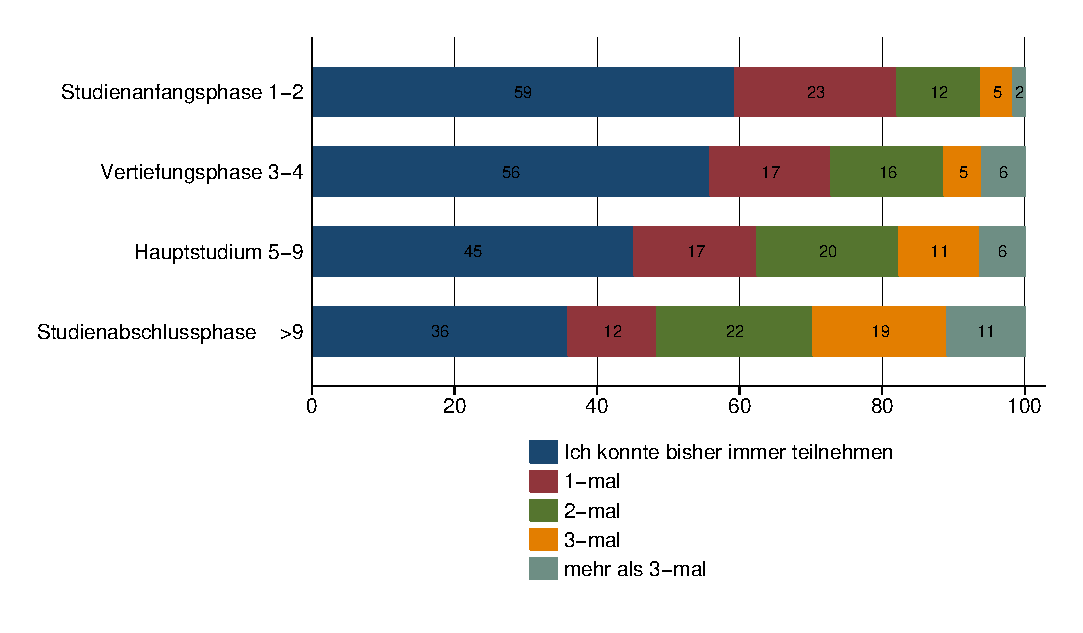
\includegraphics[RemoveGraphicsExtensions={.pdf,PDF}]{image}|
% \end{quote}
%
% \subsection{\plainTeX}
%
% \LaTeX's graphics packages can also be used with \plainTeX.
% The necessary basic \LaTeX\ macros are defined in
% \xfile{miniltx.tex}. This package \xpackage{grfext} also
% relies on it. Example:
%\begin{quote}
%\begin{verbatim}
%\input miniltx.tex\relax
%\def\Gin@driver{pdftex.def}
%\input graphicx.sty\relax
%\input grfext.sty\relax
%\resetatcatcode
%\end{verbatim}
%\end{quote}
%
% \StopEventually{
% }
%
% \section{Implementation}
%
%    \begin{macrocode}
%<*package>
%    \end{macrocode}
%
% \subsection{Relead check and identification}
%    Reload check, especially if the package is not used with \LaTeX.
%    \begin{macrocode}
\begingroup\catcode61\catcode48\catcode32=10\relax%
  \catcode13=5 % ^^M
  \endlinechar=13 %
  \catcode35=6 % #
  \catcode39=12 % '
  \catcode44=12 % ,
  \catcode45=12 % -
  \catcode46=12 % .
  \catcode58=12 % :
  \catcode64=11 % @
  \catcode123=1 % {
  \catcode125=2 % }
  \expandafter\let\expandafter\x\csname ver@grfext.sty\endcsname
  \ifx\x\relax % plain-TeX, first loading
  \else
    \def\empty{}%
    \ifx\x\empty % LaTeX, first loading,
      % variable is initialized, but \ProvidesPackage not yet seen
    \else
      \expandafter\ifx\csname PackageInfo\endcsname\relax
        \def\x#1#2{%
          \immediate\write-1{Package #1 Info: #2.}%
        }%
      \else
        \def\x#1#2{\PackageInfo{#1}{#2, stopped}}%
      \fi
      \x{grfext}{The package is already loaded}%
      \aftergroup\endinput
    \fi
  \fi
\endgroup%
%    \end{macrocode}
%    Package identification:
%    \begin{macrocode}
\begingroup\catcode61\catcode48\catcode32=10\relax%
  \catcode13=5 % ^^M
  \endlinechar=13 %
  \catcode35=6 % #
  \catcode39=12 % '
  \catcode40=12 % (
  \catcode41=12 % )
  \catcode44=12 % ,
  \catcode45=12 % -
  \catcode46=12 % .
  \catcode47=12 % /
  \catcode58=12 % :
  \catcode64=11 % @
  \catcode91=12 % [
  \catcode93=12 % ]
  \catcode123=1 % {
  \catcode125=2 % }
  \expandafter\ifx\csname ProvidesPackage\endcsname\relax
    \def\x#1#2#3[#4]{\endgroup
      \immediate\write-1{Package: #3 #4}%
      \xdef#1{#4}%
    }%
  \else
    \def\x#1#2[#3]{\endgroup
      #2[{#3}]%
      \ifx#1\@undefined
        \xdef#1{#3}%
      \fi
      \ifx#1\relax
        \xdef#1{#3}%
      \fi
    }%
  \fi
\expandafter\x\csname ver@grfext.sty\endcsname
\ProvidesPackage{grfext}%
  [2019/12/03 v1.3 Manage graphics extensions (HO)]%
%    \end{macrocode}
%
% \subsection{Catcodes}
%
%    \begin{macrocode}
\begingroup\catcode61\catcode48\catcode32=10\relax%
  \catcode13=5 % ^^M
  \endlinechar=13 %
  \catcode123=1 % {
  \catcode125=2 % }
  \catcode64=11 % @
  \def\x{\endgroup
    \expandafter\edef\csname grfext@AtEnd\endcsname{%
      \endlinechar=\the\endlinechar\relax
      \catcode13=\the\catcode13\relax
      \catcode32=\the\catcode32\relax
      \catcode35=\the\catcode35\relax
      \catcode61=\the\catcode61\relax
      \catcode64=\the\catcode64\relax
      \catcode123=\the\catcode123\relax
      \catcode125=\the\catcode125\relax
    }%
  }%
\x\catcode61\catcode48\catcode32=10\relax%
\catcode13=5 % ^^M
\endlinechar=13 %
\catcode35=6 % #
\catcode64=11 % @
\catcode123=1 % {
\catcode125=2 % }
\def\TMP@EnsureCode#1#2{%
  \edef\grfext@AtEnd{%
    \grfext@AtEnd
    \catcode#1=\the\catcode#1\relax
  }%
  \catcode#1=#2\relax
}
\TMP@EnsureCode{42}{12}% *
\TMP@EnsureCode{44}{12}% ,
\TMP@EnsureCode{47}{12}% /
\TMP@EnsureCode{58}{12}% :
\TMP@EnsureCode{60}{12}% <
\TMP@EnsureCode{62}{12}% >
\TMP@EnsureCode{91}{12}% [
\TMP@EnsureCode{93}{12}% ]
\edef\grfext@AtEnd{\grfext@AtEnd\noexpand\endinput}
%    \end{macrocode}
%
% \subsection{\plainTeX}
%
%    \begin{macro}{\@expandtwoargs}
%    Requirement is \xfile{miniltx.tex}, but we need also
%    \LaTeX's \cs{@expandtwoargs}.
%    \begin{macrocode}
\@ifundefined{@expandtwoargs}{%
  \def\@expandtwoargs#1#2#3{%
    \edef\reserved@a{\noexpand#1{#2}{#3}}%
    \reserved@a
  }%
}{}
%    \end{macrocode}
%    \end{macro}
%
% \subsection{Add}
%
%    \begin{macro}{\AppendGraphicsExtensions}
%    \begin{macrocode}
\newcommand*{\AppendGraphicsExtensions}{%
  \@ifundefined{Gin@extensions}{%
    \let\Gin@extensions\@empty
  }{}%
  \@ifstar{\grfext@Append\grfext@Check}{\grfext@Append\grfext@@Add}%
}%
%    \end{macrocode}
%    \end{macro}
%    \begin{macro}{\grfext@Append}
%    \begin{macrocode}
\def\grfext@Append#1#2{%
  \let\grfext@Print\@gobble
  \edef\grfext@next{%
    \noexpand\grfext@Add\noexpand#1{%
      \zap@space#2 \@empty
    }{\noexpand\Gin@extensions,}{}%
  }%
  \grfext@next
  \let\grfext@Print\grfext@@Print
  \grfext@Print\AppendGraphicsExtensions
}
%    \end{macrocode}
%    \end{macro}
%
%    \begin{macro}{\PrependGraphicsExtensions}
%    \begin{macrocode}
\newcommand*{\PrependGraphicsExtensions}{%
  \@ifundefined{Gin@extensions}{%
    \let\Gin@extensions\@empty
  }{}%
  \@ifstar{\grfext@Prepend\grfext@Check}{\grfext@Prepend\grfext@@Add}%
}%
%    \end{macrocode}
%    \end{macro}
%    \begin{macro}{\grfext@Prepend}
%    \begin{macrocode}
\def\grfext@Prepend#1#2{%
  \let\grfext@Print\@gobble
  \edef\grfext@next{%
    \noexpand\grfext@Add\noexpand#1{%
      \zap@space#2 \@empty
    }{}{,\noexpand\Gin@extensions}%
  }%
  \grfext@next
  \let\grfext@Print\grfext@@Print
  \grfext@Print\PrependGraphicsExtensions
}
%    \end{macrocode}
%    \end{macro}
%
%    \begin{macro}{\grfext@Add}
%    \begin{macrocode}
\def\grfext@Add#1#2{%
  #1{#2}%
}
%    \end{macrocode}
%    \end{macro}
%    \begin{macro}{\grfext@@Add}
%    \begin{macrocode}
\def\grfext@@Add#1#2#3{%
  \RemoveGraphicsExtensions{#1}%
  \ifx\Gin@extensions\@empty
    \def\Gin@extensions{#1}%
  \else
    \edef\Gin@extensions{#2#1#3}%
  \fi
}
%    \end{macrocode}
%    \end{macro}
%
% \subsection{Check}
%
%    \begin{macro}{\grfext@Check}
%    \begin{macrocode}
\def\grfext@Check#1{%
  \let\grfext@tmp\@empty
  \@for\grfext@ext:=#1\do{%
    \@ifundefined{Gin@rule@\grfext@ext}{%
    }{%
      \ifx\grfext@tmp\@empty
        \let\grfext@tmp\grfext@ext
      \else
        \edef\grfext@tmp{\grfext@tmp,\grfext@ext}%
      \fi
    }%
  }%
  \ifx\grfext@tmp\@empty
    \def\grfext@next##1##2{}%
  \else
    \edef\grfext@next{%
      \noexpand\grfext@@Add{\grfext@tmp}%
    }%
  \fi
  \grfext@next
}
%    \end{macrocode}
%    \end{macro}
%
% \subsection{Remove}
%
%    \begin{macro}{\RemoveGraphicsExtensions}
%    \begin{macrocode}
\newcommand*{\RemoveGraphicsExtensions}[1]{%
  \@ifundefined{Gin@extensions}{%
    \def\Gin@extensions{}%
  }{%
    \edef\grfext@tmp{\zap@space#1 \@empty}%
    \@for\grfext@ext:=\grfext@tmp\do{%
      \def\grfext@next{%
        \let\grfext@tmp\Gin@extensions
        \@expandtwoargs
        \@removeelement\grfext@ext\Gin@extensions\Gin@extensions
        \ifx\grfext@tmp\Gin@extensions
          \let\grfext@next\relax
        \fi
        \grfext@next
      }%
      \grfext@next
    }%
  }%
  \grfext@Print\RemoveGraphicsExtensions
}
%    \end{macrocode}
%    \end{macro}
%
% \subsection{Print}
%
%    \begin{macrocode}
\RequirePackage{infwarerr}[2007/09/09]
%    \end{macrocode}
%
%    \begin{macro}{\PrintGraphicsExtensions}
%    \begin{macrocode}
\def\PrintGraphicsExtensions{%
  \grfext@Print\PrintGraphicsExtensions
}
%    \end{macrocode}
%    \end{macro}
%    \begin{macro}{\grfext@Print}
%    \begin{macrocode}
\def\grfext@Print#1{%
  \@PackageInfo{grfext}{%
    Graphics extension search list:\MessageBreak
    \@ifundefined{Gin@extensions}{%
      <unavailable>%
    }{%
      [\Gin@extensions]%
    }\MessageBreak
    \string#1%
  }%
}
%    \end{macrocode}
%    \end{macro}
%    \begin{macro}{\grfext@@Print}
%    \begin{macrocode}
\let\grfext@@Print\grfext@Print
%    \end{macrocode}
%    \end{macro}
%
% \subsection{Defining options for package \xpackage{graphicx}}
%
%    \begin{macrocode}
\RequirePackage{kvdefinekeys}[2010/03/01]
\kv@define@key{Gin}{AppendGraphicsExtensions}{%
  \AppendGraphicsExtensions{#1}%
}
\kv@define@key{Gin}{AppendGraphicsExtensions*}{%
  \AppendGraphicsExtensions*{#1}%
}
\kv@define@key{Gin}{PrependGraphicsExtensions}{%
  \PrependGraphicsExtensions{#1}%
}
\kv@define@key{Gin}{PrependGraphicsExtensions*}{%
  \PrependGraphicsExtensions*{#1}%
}
\kv@define@key{Gin}{RemoveGraphicsExtensions}{%
  \RemoveGraphicsExtensions{#1}%
}
\kv@define@key{Gin}{PrintGraphicsExtensions}[]{%
  \PrintGraphicsExtensions
}
%    \end{macrocode}
%
%    \begin{macrocode}
\grfext@AtEnd%
%</package>
%    \end{macrocode}
% \section{Installation}
%
% \subsection{Download}
%
% \paragraph{Package.} This package is available on
% CTAN\footnote{\CTANpkg{grfext}}:
% \begin{description}
% \item[\CTAN{macros/latex/contrib/grfext/grfext.dtx}] The source file.
% \item[\CTAN{macros/latex/contrib/grfext/grfext.pdf}] Documentation.
% \end{description}
%
%
% \paragraph{Bundle.} All the packages of the bundle `grfext'
% are also available in a TDS compliant ZIP archive. There
% the packages are already unpacked and the documentation files
% are generated. The files and directories obey the TDS standard.
% \begin{description}
% \item[\CTANinstall{install/macros/latex/contrib/grfext.tds.zip}]
% \end{description}
% \emph{TDS} refers to the standard ``A Directory Structure
% for \TeX\ Files'' (\CTANpkg{tds}). Directories
% with \xfile{texmf} in their name are usually organized this way.
%
% \subsection{Bundle installation}
%
% \paragraph{Unpacking.} Unpack the \xfile{grfext.tds.zip} in the
% TDS tree (also known as \xfile{texmf} tree) of your choice.
% Example (linux):
% \begin{quote}
%   |unzip grfext.tds.zip -d ~/texmf|
% \end{quote}
%
% \subsection{Package installation}
%
% \paragraph{Unpacking.} The \xfile{.dtx} file is a self-extracting
% \docstrip\ archive. The files are extracted by running the
% \xfile{.dtx} through \plainTeX:
% \begin{quote}
%   \verb|tex grfext.dtx|
% \end{quote}
%
% \paragraph{TDS.} Now the different files must be moved into
% the different directories in your installation TDS tree
% (also known as \xfile{texmf} tree):
% \begin{quote}
% \def\t{^^A
% \begin{tabular}{@{}>{\ttfamily}l@{ $\rightarrow$ }>{\ttfamily}l@{}}
%   grfext.sty & tex/latex/grfext/grfext.sty\\
%   grfext.pdf & doc/latex/grfext/grfext.pdf\\
%   grfext.dtx & source/latex/grfext/grfext.dtx\\
% \end{tabular}^^A
% }^^A
% \sbox0{\t}^^A
% \ifdim\wd0>\linewidth
%   \begingroup
%     \advance\linewidth by\leftmargin
%     \advance\linewidth by\rightmargin
%   \edef\x{\endgroup
%     \def\noexpand\lw{\the\linewidth}^^A
%   }\x
%   \def\lwbox{^^A
%     \leavevmode
%     \hbox to \linewidth{^^A
%       \kern-\leftmargin\relax
%       \hss
%       \usebox0
%       \hss
%       \kern-\rightmargin\relax
%     }^^A
%   }^^A
%   \ifdim\wd0>\lw
%     \sbox0{\small\t}^^A
%     \ifdim\wd0>\linewidth
%       \ifdim\wd0>\lw
%         \sbox0{\footnotesize\t}^^A
%         \ifdim\wd0>\linewidth
%           \ifdim\wd0>\lw
%             \sbox0{\scriptsize\t}^^A
%             \ifdim\wd0>\linewidth
%               \ifdim\wd0>\lw
%                 \sbox0{\tiny\t}^^A
%                 \ifdim\wd0>\linewidth
%                   \lwbox
%                 \else
%                   \usebox0
%                 \fi
%               \else
%                 \lwbox
%               \fi
%             \else
%               \usebox0
%             \fi
%           \else
%             \lwbox
%           \fi
%         \else
%           \usebox0
%         \fi
%       \else
%         \lwbox
%       \fi
%     \else
%       \usebox0
%     \fi
%   \else
%     \lwbox
%   \fi
% \else
%   \usebox0
% \fi
% \end{quote}
% If you have a \xfile{docstrip.cfg} that configures and enables \docstrip's
% TDS installing feature, then some files can already be in the right
% place, see the documentation of \docstrip.
%
% \subsection{Refresh file name databases}
%
% If your \TeX~distribution
% (\TeX\,Live, \mikTeX, \dots) relies on file name databases, you must refresh
% these. For example, \TeX\,Live\ users run \verb|texhash| or
% \verb|mktexlsr|.
%
% \subsection{Some details for the interested}
%
% \paragraph{Unpacking with \LaTeX.}
% The \xfile{.dtx} chooses its action depending on the format:
% \begin{description}
% \item[\plainTeX:] Run \docstrip\ and extract the files.
% \item[\LaTeX:] Generate the documentation.
% \end{description}
% If you insist on using \LaTeX\ for \docstrip\ (really,
% \docstrip\ does not need \LaTeX), then inform the autodetect routine
% about your intention:
% \begin{quote}
%   \verb|latex \let\install=y\input{grfext.dtx}|
% \end{quote}
% Do not forget to quote the argument according to the demands
% of your shell.
%
% \paragraph{Generating the documentation.}
% You can use both the \xfile{.dtx} or the \xfile{.drv} to generate
% the documentation. The process can be configured by the
% configuration file \xfile{ltxdoc.cfg}. For instance, put this
% line into this file, if you want to have A4 as paper format:
% \begin{quote}
%   \verb|\PassOptionsToClass{a4paper}{article}|
% \end{quote}
% An example follows how to generate the
% documentation with pdf\LaTeX:
% \begin{quote}
%\begin{verbatim}
%pdflatex grfext.dtx
%makeindex -s gind.ist grfext.idx
%pdflatex grfext.dtx
%makeindex -s gind.ist grfext.idx
%pdflatex grfext.dtx
%\end{verbatim}
% \end{quote}
%
% \begin{thebibliography}{9}
%
% \bibitem{graphics}
%   David Carlisle, Sebastian Rahtz: \textit{The \xpackage{graphics} package};
%   2006/02/20 v1.0o;
%   \CTAN{macros/latex/required/graphics/graphics.dtx}.
%
% \end{thebibliography}
%
% \begin{History}
%   \begin{Version}{2007/09/30 v1.0}
%   \item
%     First public version.
%   \end{Version}
%   \begin{Version}{2010/08/19 v1.1}
%   \item
%     User macros are also made available as keyval options for
%     package \xpackage{graphicx}.
%   \end{Version}
%   \begin{Version}{2016/05/16 v1.2}
%   \item
%     Documentation updates.
%   \end{Version}
%   \begin{Version}{2019/12/03 v1.3}
%   \item
%     Documentation updates.
%   \end{Version}
% \end{History}
%
% \PrintIndex
%
% \Finale
\endinput

%        (quote the arguments according to the demands of your shell)
%
% Documentation:
%    (a) If grfext.drv is present:
%           latex grfext.drv
%    (b) Without grfext.drv:
%           latex grfext.dtx; ...
%    The class ltxdoc loads the configuration file ltxdoc.cfg
%    if available. Here you can specify further options, e.g.
%    use A4 as paper format:
%       \PassOptionsToClass{a4paper}{article}
%
%    Programm calls to get the documentation (example):
%       pdflatex grfext.dtx
%       makeindex -s gind.ist grfext.idx
%       pdflatex grfext.dtx
%       makeindex -s gind.ist grfext.idx
%       pdflatex grfext.dtx
%
% Installation:
%    TDS:tex/latex/grfext/grfext.sty
%    TDS:doc/latex/grfext/grfext.pdf
%    TDS:source/latex/grfext/grfext.dtx
%
%<*ignore>
\begingroup
  \catcode123=1 %
  \catcode125=2 %
  \def\x{LaTeX2e}%
\expandafter\endgroup
\ifcase 0\ifx\install y1\fi\expandafter
         \ifx\csname processbatchFile\endcsname\relax\else1\fi
         \ifx\fmtname\x\else 1\fi\relax
\else\csname fi\endcsname
%</ignore>
%<*install>
\input docstrip.tex
\Msg{************************************************************************}
\Msg{* Installation}
\Msg{* Package: grfext 2019/12/03 v1.3 Manage graphics extensions (HO)}
\Msg{************************************************************************}

\keepsilent
\askforoverwritefalse

\let\MetaPrefix\relax
\preamble

This is a generated file.

Project: grfext
Version: 2019/12/03 v1.3

Copyright (C)
   2007, 2010 Heiko Oberdiek
   2016-2019 Oberdiek Package Support Group

This work may be distributed and/or modified under the
conditions of the LaTeX Project Public License, either
version 1.3c of this license or (at your option) any later
version. This version of this license is in
   https://www.latex-project.org/lppl/lppl-1-3c.txt
and the latest version of this license is in
   https://www.latex-project.org/lppl.txt
and version 1.3 or later is part of all distributions of
LaTeX version 2005/12/01 or later.

This work has the LPPL maintenance status "maintained".

The Current Maintainers of this work are
Heiko Oberdiek and the Oberdiek Package Support Group
https://github.com/ho-tex/grfext/issues


This work consists of the main source file grfext.dtx
and the derived files
   grfext.sty, grfext.pdf, grfext.ins, grfext.drv.

\endpreamble
\let\MetaPrefix\DoubleperCent

\generate{%
  \file{grfext.ins}{\from{grfext.dtx}{install}}%
  \file{grfext.drv}{\from{grfext.dtx}{driver}}%
  \usedir{tex/latex/grfext}%
  \file{grfext.sty}{\from{grfext.dtx}{package}}%
%  \usedir{doc/latex/grfext/test}%
%  \file{grfext-test1.tex}{\from{grfext.dtx}{test1}}%
%  \file{grfext-test2.tex}{\from{grfext.dtx}{test2}}%
}

\catcode32=13\relax% active space
\let =\space%
\Msg{************************************************************************}
\Msg{*}
\Msg{* To finish the installation you have to move the following}
\Msg{* file into a directory searched by TeX:}
\Msg{*}
\Msg{*     grfext.sty}
\Msg{*}
\Msg{* To produce the documentation run the file `grfext.drv'}
\Msg{* through LaTeX.}
\Msg{*}
\Msg{* Happy TeXing!}
\Msg{*}
\Msg{************************************************************************}

\endbatchfile
%</install>
%<*ignore>
\fi
%</ignore>
%<*driver>
\NeedsTeXFormat{LaTeX2e}
\ProvidesFile{grfext.drv}%
  [2019/12/03 v1.3 Manage graphics extensions (HO)]%
\documentclass{ltxdoc}
\usepackage{holtxdoc}[2011/11/22]
\begin{document}
  \DocInput{grfext.dtx}%
\end{document}
%</driver>
% \fi
%
%
%
% \GetFileInfo{grfext.drv}
%
% \title{The \xpackage{grfext} package}
% \date{2019/12/03 v1.3}
% \author{Heiko Oberdiek\thanks
% {Please report any issues at \url{https://github.com/ho-tex/grfext/issues}}}
%
% \maketitle
%
% \begin{abstract}
% This package provides macros for adding and reordering
% graphics extensions of package \xpackage{graphics}.
% \end{abstract}
%
% \tableofcontents
%
% \section{Documentation}
%
% \subsection{Introduction}
%
% If you are not familiar with \LaTeX's graphics bundle, please
% read its documentation \xfile{grffile} \cite{graphics}.
% The bundle contains two packages for graphics inclusion:
% \xpackage{graphics} and \xpackage{graphicx}. The first one
% is loaded by the second one that adds a key value interface.
%
% Graphics files are included in both cases by macro
% \cs{includegraphics}. The file name extension can be omitted.
% Then the graphics package goes through a list of known
% extensions until it finds the graphics file. This extension list
% is set by \cs{DeclareGraphicsExtensions}. The previous contents
% of the list is overwritten.
%
% \subsection{User interface}
%
% This package \xpackage{grfext} provides macros that adds entries
% to the list or remove them. The list may be empty or even
% undefined before. It is always defined afterwards, but can
% be empty (especially after removing entries).
%
% \begin{declcs}{AppendGraphicsExtensions} * \M{ext-list}\\
%   \cs{PrependGraphicsExtensions} * \M{ext-list}
% \end{declcs}
% The argument \meta{ext-list} is a comma separated list whose
% entries are file name extensions including the dot.
% But first the entries are removed from
% \xpackage{graphics}' extension list to avoid multiple
% occurences of the same extension.
%
% Then macro \cs{AppendGraphicsExtensions} adds the entries
% after the end of \xpackage{graphics}' list, whereas
% macro \cs{PrependGraphicsExtensions} puts them in front
% of the list.
% The order matters if a graphics file is available in
% different acceptable formats. Then the first extension
% wins.
%
% The star version of these commands only adds an extensions,
% if a specific graphics rule exists for that extension.
%
% \begin{declcs}{RemoveGraphicsExtensions} \M{ext-list}
% \end{declcs}
% All occurences of file extensions in \meta{ext-list} are
% removed from \xpackage{graphics}' extension list.
%
% \subsection{Package loading}
%
% The package does not define any options. It is loaded
% as usual in \LaTeX, e.g.:
% \begin{quote}
%   |\usepackage{grfext}|
% \end{quote}
%
% \begin{declcs}{PrintGraphicsExtensions}
% \end{declcs}
% Macro \cs{PrintGraphicsExtensions} writes the current
% graphics extensions list in the \xfile{.log} file.
% The macros described before do this automatically
% after their operation.
%
% \subsection{Option support for package \xpackage{graphicx}}
%
% Package \xpackage{graphicx} uses the interface of package
% \xpackage{keyval} in order to specify options for
% \cs{includegraphics}. The options can also be set using
% \begin{quote}
%   |\setkeys{Gin}{|\meta{options}|}|
% \end{quote}
% The four user macros with the two star forms are available
% as options in family |Gin| as well:
% \begin{quote}
%   |AppendGraphicsExtensions={|\meta{ext-list}|}|\\
%   |AppendGraphicsExtensions*={|\meta{ext-list}|}|\\
%   |PrependGraphicsExtensions={|\meta{ext-list}|}|\\
%   |PrependGraphicsExtensions*{|\meta{ext-list}|}|\\
%   |RemoveGraphicsExtensions={|\meta{ext-list}|}|\\
%   |PrintGraphicsExtensions|
% \end{quote}
% This makes it easier to locally change the extension list
% for an included graphics, e.g.:
% \begin{quote}
%   |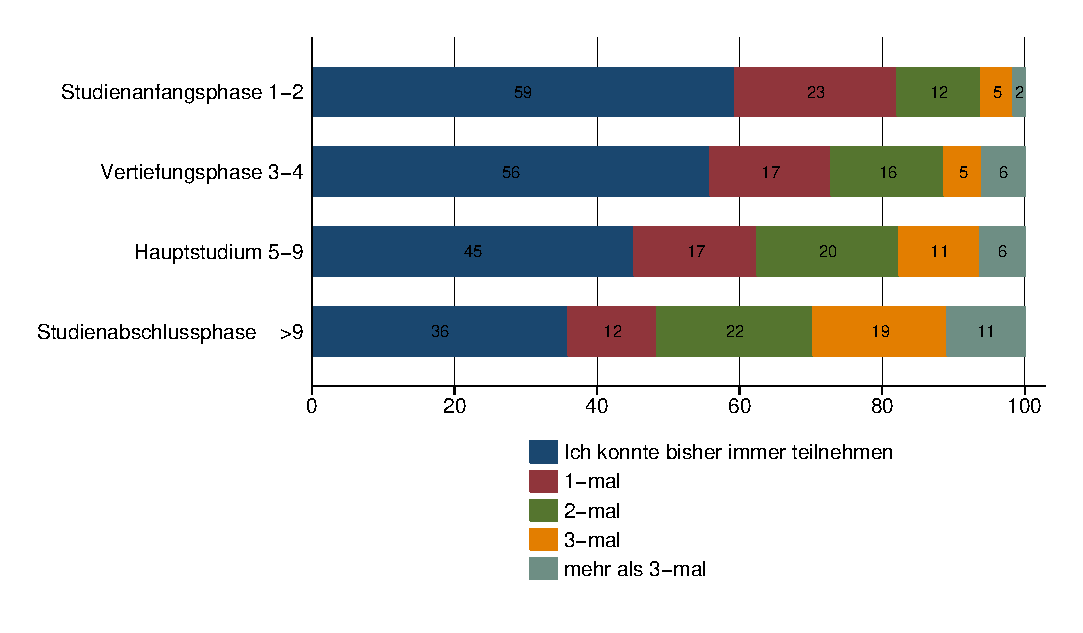
\includegraphics[RemoveGraphicsExtensions={.pdf,PDF}]{image}|
% \end{quote}
%
% \subsection{\plainTeX}
%
% \LaTeX's graphics packages can also be used with \plainTeX.
% The necessary basic \LaTeX\ macros are defined in
% \xfile{miniltx.tex}. This package \xpackage{grfext} also
% relies on it. Example:
%\begin{quote}
%\begin{verbatim}
%\input miniltx.tex\relax
%\def\Gin@driver{pdftex.def}
%\input graphicx.sty\relax
%\input grfext.sty\relax
%\resetatcatcode
%\end{verbatim}
%\end{quote}
%
% \StopEventually{
% }
%
% \section{Implementation}
%
%    \begin{macrocode}
%<*package>
%    \end{macrocode}
%
% \subsection{Relead check and identification}
%    Reload check, especially if the package is not used with \LaTeX.
%    \begin{macrocode}
\begingroup\catcode61\catcode48\catcode32=10\relax%
  \catcode13=5 % ^^M
  \endlinechar=13 %
  \catcode35=6 % #
  \catcode39=12 % '
  \catcode44=12 % ,
  \catcode45=12 % -
  \catcode46=12 % .
  \catcode58=12 % :
  \catcode64=11 % @
  \catcode123=1 % {
  \catcode125=2 % }
  \expandafter\let\expandafter\x\csname ver@grfext.sty\endcsname
  \ifx\x\relax % plain-TeX, first loading
  \else
    \def\empty{}%
    \ifx\x\empty % LaTeX, first loading,
      % variable is initialized, but \ProvidesPackage not yet seen
    \else
      \expandafter\ifx\csname PackageInfo\endcsname\relax
        \def\x#1#2{%
          \immediate\write-1{Package #1 Info: #2.}%
        }%
      \else
        \def\x#1#2{\PackageInfo{#1}{#2, stopped}}%
      \fi
      \x{grfext}{The package is already loaded}%
      \aftergroup\endinput
    \fi
  \fi
\endgroup%
%    \end{macrocode}
%    Package identification:
%    \begin{macrocode}
\begingroup\catcode61\catcode48\catcode32=10\relax%
  \catcode13=5 % ^^M
  \endlinechar=13 %
  \catcode35=6 % #
  \catcode39=12 % '
  \catcode40=12 % (
  \catcode41=12 % )
  \catcode44=12 % ,
  \catcode45=12 % -
  \catcode46=12 % .
  \catcode47=12 % /
  \catcode58=12 % :
  \catcode64=11 % @
  \catcode91=12 % [
  \catcode93=12 % ]
  \catcode123=1 % {
  \catcode125=2 % }
  \expandafter\ifx\csname ProvidesPackage\endcsname\relax
    \def\x#1#2#3[#4]{\endgroup
      \immediate\write-1{Package: #3 #4}%
      \xdef#1{#4}%
    }%
  \else
    \def\x#1#2[#3]{\endgroup
      #2[{#3}]%
      \ifx#1\@undefined
        \xdef#1{#3}%
      \fi
      \ifx#1\relax
        \xdef#1{#3}%
      \fi
    }%
  \fi
\expandafter\x\csname ver@grfext.sty\endcsname
\ProvidesPackage{grfext}%
  [2019/12/03 v1.3 Manage graphics extensions (HO)]%
%    \end{macrocode}
%
% \subsection{Catcodes}
%
%    \begin{macrocode}
\begingroup\catcode61\catcode48\catcode32=10\relax%
  \catcode13=5 % ^^M
  \endlinechar=13 %
  \catcode123=1 % {
  \catcode125=2 % }
  \catcode64=11 % @
  \def\x{\endgroup
    \expandafter\edef\csname grfext@AtEnd\endcsname{%
      \endlinechar=\the\endlinechar\relax
      \catcode13=\the\catcode13\relax
      \catcode32=\the\catcode32\relax
      \catcode35=\the\catcode35\relax
      \catcode61=\the\catcode61\relax
      \catcode64=\the\catcode64\relax
      \catcode123=\the\catcode123\relax
      \catcode125=\the\catcode125\relax
    }%
  }%
\x\catcode61\catcode48\catcode32=10\relax%
\catcode13=5 % ^^M
\endlinechar=13 %
\catcode35=6 % #
\catcode64=11 % @
\catcode123=1 % {
\catcode125=2 % }
\def\TMP@EnsureCode#1#2{%
  \edef\grfext@AtEnd{%
    \grfext@AtEnd
    \catcode#1=\the\catcode#1\relax
  }%
  \catcode#1=#2\relax
}
\TMP@EnsureCode{42}{12}% *
\TMP@EnsureCode{44}{12}% ,
\TMP@EnsureCode{47}{12}% /
\TMP@EnsureCode{58}{12}% :
\TMP@EnsureCode{60}{12}% <
\TMP@EnsureCode{62}{12}% >
\TMP@EnsureCode{91}{12}% [
\TMP@EnsureCode{93}{12}% ]
\edef\grfext@AtEnd{\grfext@AtEnd\noexpand\endinput}
%    \end{macrocode}
%
% \subsection{\plainTeX}
%
%    \begin{macro}{\@expandtwoargs}
%    Requirement is \xfile{miniltx.tex}, but we need also
%    \LaTeX's \cs{@expandtwoargs}.
%    \begin{macrocode}
\@ifundefined{@expandtwoargs}{%
  \def\@expandtwoargs#1#2#3{%
    \edef\reserved@a{\noexpand#1{#2}{#3}}%
    \reserved@a
  }%
}{}
%    \end{macrocode}
%    \end{macro}
%
% \subsection{Add}
%
%    \begin{macro}{\AppendGraphicsExtensions}
%    \begin{macrocode}
\newcommand*{\AppendGraphicsExtensions}{%
  \@ifundefined{Gin@extensions}{%
    \let\Gin@extensions\@empty
  }{}%
  \@ifstar{\grfext@Append\grfext@Check}{\grfext@Append\grfext@@Add}%
}%
%    \end{macrocode}
%    \end{macro}
%    \begin{macro}{\grfext@Append}
%    \begin{macrocode}
\def\grfext@Append#1#2{%
  \let\grfext@Print\@gobble
  \edef\grfext@next{%
    \noexpand\grfext@Add\noexpand#1{%
      \zap@space#2 \@empty
    }{\noexpand\Gin@extensions,}{}%
  }%
  \grfext@next
  \let\grfext@Print\grfext@@Print
  \grfext@Print\AppendGraphicsExtensions
}
%    \end{macrocode}
%    \end{macro}
%
%    \begin{macro}{\PrependGraphicsExtensions}
%    \begin{macrocode}
\newcommand*{\PrependGraphicsExtensions}{%
  \@ifundefined{Gin@extensions}{%
    \let\Gin@extensions\@empty
  }{}%
  \@ifstar{\grfext@Prepend\grfext@Check}{\grfext@Prepend\grfext@@Add}%
}%
%    \end{macrocode}
%    \end{macro}
%    \begin{macro}{\grfext@Prepend}
%    \begin{macrocode}
\def\grfext@Prepend#1#2{%
  \let\grfext@Print\@gobble
  \edef\grfext@next{%
    \noexpand\grfext@Add\noexpand#1{%
      \zap@space#2 \@empty
    }{}{,\noexpand\Gin@extensions}%
  }%
  \grfext@next
  \let\grfext@Print\grfext@@Print
  \grfext@Print\PrependGraphicsExtensions
}
%    \end{macrocode}
%    \end{macro}
%
%    \begin{macro}{\grfext@Add}
%    \begin{macrocode}
\def\grfext@Add#1#2{%
  #1{#2}%
}
%    \end{macrocode}
%    \end{macro}
%    \begin{macro}{\grfext@@Add}
%    \begin{macrocode}
\def\grfext@@Add#1#2#3{%
  \RemoveGraphicsExtensions{#1}%
  \ifx\Gin@extensions\@empty
    \def\Gin@extensions{#1}%
  \else
    \edef\Gin@extensions{#2#1#3}%
  \fi
}
%    \end{macrocode}
%    \end{macro}
%
% \subsection{Check}
%
%    \begin{macro}{\grfext@Check}
%    \begin{macrocode}
\def\grfext@Check#1{%
  \let\grfext@tmp\@empty
  \@for\grfext@ext:=#1\do{%
    \@ifundefined{Gin@rule@\grfext@ext}{%
    }{%
      \ifx\grfext@tmp\@empty
        \let\grfext@tmp\grfext@ext
      \else
        \edef\grfext@tmp{\grfext@tmp,\grfext@ext}%
      \fi
    }%
  }%
  \ifx\grfext@tmp\@empty
    \def\grfext@next##1##2{}%
  \else
    \edef\grfext@next{%
      \noexpand\grfext@@Add{\grfext@tmp}%
    }%
  \fi
  \grfext@next
}
%    \end{macrocode}
%    \end{macro}
%
% \subsection{Remove}
%
%    \begin{macro}{\RemoveGraphicsExtensions}
%    \begin{macrocode}
\newcommand*{\RemoveGraphicsExtensions}[1]{%
  \@ifundefined{Gin@extensions}{%
    \def\Gin@extensions{}%
  }{%
    \edef\grfext@tmp{\zap@space#1 \@empty}%
    \@for\grfext@ext:=\grfext@tmp\do{%
      \def\grfext@next{%
        \let\grfext@tmp\Gin@extensions
        \@expandtwoargs
        \@removeelement\grfext@ext\Gin@extensions\Gin@extensions
        \ifx\grfext@tmp\Gin@extensions
          \let\grfext@next\relax
        \fi
        \grfext@next
      }%
      \grfext@next
    }%
  }%
  \grfext@Print\RemoveGraphicsExtensions
}
%    \end{macrocode}
%    \end{macro}
%
% \subsection{Print}
%
%    \begin{macrocode}
\RequirePackage{infwarerr}[2007/09/09]
%    \end{macrocode}
%
%    \begin{macro}{\PrintGraphicsExtensions}
%    \begin{macrocode}
\def\PrintGraphicsExtensions{%
  \grfext@Print\PrintGraphicsExtensions
}
%    \end{macrocode}
%    \end{macro}
%    \begin{macro}{\grfext@Print}
%    \begin{macrocode}
\def\grfext@Print#1{%
  \@PackageInfo{grfext}{%
    Graphics extension search list:\MessageBreak
    \@ifundefined{Gin@extensions}{%
      <unavailable>%
    }{%
      [\Gin@extensions]%
    }\MessageBreak
    \string#1%
  }%
}
%    \end{macrocode}
%    \end{macro}
%    \begin{macro}{\grfext@@Print}
%    \begin{macrocode}
\let\grfext@@Print\grfext@Print
%    \end{macrocode}
%    \end{macro}
%
% \subsection{Defining options for package \xpackage{graphicx}}
%
%    \begin{macrocode}
\RequirePackage{kvdefinekeys}[2010/03/01]
\kv@define@key{Gin}{AppendGraphicsExtensions}{%
  \AppendGraphicsExtensions{#1}%
}
\kv@define@key{Gin}{AppendGraphicsExtensions*}{%
  \AppendGraphicsExtensions*{#1}%
}
\kv@define@key{Gin}{PrependGraphicsExtensions}{%
  \PrependGraphicsExtensions{#1}%
}
\kv@define@key{Gin}{PrependGraphicsExtensions*}{%
  \PrependGraphicsExtensions*{#1}%
}
\kv@define@key{Gin}{RemoveGraphicsExtensions}{%
  \RemoveGraphicsExtensions{#1}%
}
\kv@define@key{Gin}{PrintGraphicsExtensions}[]{%
  \PrintGraphicsExtensions
}
%    \end{macrocode}
%
%    \begin{macrocode}
\grfext@AtEnd%
%</package>
%    \end{macrocode}
% \section{Installation}
%
% \subsection{Download}
%
% \paragraph{Package.} This package is available on
% CTAN\footnote{\CTANpkg{grfext}}:
% \begin{description}
% \item[\CTAN{macros/latex/contrib/grfext/grfext.dtx}] The source file.
% \item[\CTAN{macros/latex/contrib/grfext/grfext.pdf}] Documentation.
% \end{description}
%
%
% \paragraph{Bundle.} All the packages of the bundle `grfext'
% are also available in a TDS compliant ZIP archive. There
% the packages are already unpacked and the documentation files
% are generated. The files and directories obey the TDS standard.
% \begin{description}
% \item[\CTANinstall{install/macros/latex/contrib/grfext.tds.zip}]
% \end{description}
% \emph{TDS} refers to the standard ``A Directory Structure
% for \TeX\ Files'' (\CTANpkg{tds}). Directories
% with \xfile{texmf} in their name are usually organized this way.
%
% \subsection{Bundle installation}
%
% \paragraph{Unpacking.} Unpack the \xfile{grfext.tds.zip} in the
% TDS tree (also known as \xfile{texmf} tree) of your choice.
% Example (linux):
% \begin{quote}
%   |unzip grfext.tds.zip -d ~/texmf|
% \end{quote}
%
% \subsection{Package installation}
%
% \paragraph{Unpacking.} The \xfile{.dtx} file is a self-extracting
% \docstrip\ archive. The files are extracted by running the
% \xfile{.dtx} through \plainTeX:
% \begin{quote}
%   \verb|tex grfext.dtx|
% \end{quote}
%
% \paragraph{TDS.} Now the different files must be moved into
% the different directories in your installation TDS tree
% (also known as \xfile{texmf} tree):
% \begin{quote}
% \def\t{^^A
% \begin{tabular}{@{}>{\ttfamily}l@{ $\rightarrow$ }>{\ttfamily}l@{}}
%   grfext.sty & tex/latex/grfext/grfext.sty\\
%   grfext.pdf & doc/latex/grfext/grfext.pdf\\
%   grfext.dtx & source/latex/grfext/grfext.dtx\\
% \end{tabular}^^A
% }^^A
% \sbox0{\t}^^A
% \ifdim\wd0>\linewidth
%   \begingroup
%     \advance\linewidth by\leftmargin
%     \advance\linewidth by\rightmargin
%   \edef\x{\endgroup
%     \def\noexpand\lw{\the\linewidth}^^A
%   }\x
%   \def\lwbox{^^A
%     \leavevmode
%     \hbox to \linewidth{^^A
%       \kern-\leftmargin\relax
%       \hss
%       \usebox0
%       \hss
%       \kern-\rightmargin\relax
%     }^^A
%   }^^A
%   \ifdim\wd0>\lw
%     \sbox0{\small\t}^^A
%     \ifdim\wd0>\linewidth
%       \ifdim\wd0>\lw
%         \sbox0{\footnotesize\t}^^A
%         \ifdim\wd0>\linewidth
%           \ifdim\wd0>\lw
%             \sbox0{\scriptsize\t}^^A
%             \ifdim\wd0>\linewidth
%               \ifdim\wd0>\lw
%                 \sbox0{\tiny\t}^^A
%                 \ifdim\wd0>\linewidth
%                   \lwbox
%                 \else
%                   \usebox0
%                 \fi
%               \else
%                 \lwbox
%               \fi
%             \else
%               \usebox0
%             \fi
%           \else
%             \lwbox
%           \fi
%         \else
%           \usebox0
%         \fi
%       \else
%         \lwbox
%       \fi
%     \else
%       \usebox0
%     \fi
%   \else
%     \lwbox
%   \fi
% \else
%   \usebox0
% \fi
% \end{quote}
% If you have a \xfile{docstrip.cfg} that configures and enables \docstrip's
% TDS installing feature, then some files can already be in the right
% place, see the documentation of \docstrip.
%
% \subsection{Refresh file name databases}
%
% If your \TeX~distribution
% (\TeX\,Live, \mikTeX, \dots) relies on file name databases, you must refresh
% these. For example, \TeX\,Live\ users run \verb|texhash| or
% \verb|mktexlsr|.
%
% \subsection{Some details for the interested}
%
% \paragraph{Unpacking with \LaTeX.}
% The \xfile{.dtx} chooses its action depending on the format:
% \begin{description}
% \item[\plainTeX:] Run \docstrip\ and extract the files.
% \item[\LaTeX:] Generate the documentation.
% \end{description}
% If you insist on using \LaTeX\ for \docstrip\ (really,
% \docstrip\ does not need \LaTeX), then inform the autodetect routine
% about your intention:
% \begin{quote}
%   \verb|latex \let\install=y% \iffalse meta-comment
%
% File: grfext.dtx
% Version: 2019/12/03 v1.3
% Info: Manage graphics extensions
%
% Copyright (C)
%    2007, 2010 Heiko Oberdiek
%    2016-2019 Oberdiek Package Support Group
%    https://github.com/ho-tex/grfext/issues
%
% This work may be distributed and/or modified under the
% conditions of the LaTeX Project Public License, either
% version 1.3c of this license or (at your option) any later
% version. This version of this license is in
%    https://www.latex-project.org/lppl/lppl-1-3c.txt
% and the latest version of this license is in
%    https://www.latex-project.org/lppl.txt
% and version 1.3 or later is part of all distributions of
% LaTeX version 2005/12/01 or later.
%
% This work has the LPPL maintenance status "maintained".
%
% The Current Maintainers of this work are
% Heiko Oberdiek and the Oberdiek Package Support Group
% https://github.com/ho-tex/grfext/issues
%
% This work consists of the main source file grfext.dtx
% and the derived files
%    grfext.sty, grfext.pdf, grfext.ins, grfext.drv,
%
% Distribution:
%    CTAN:macros/latex/contrib/grfext/grfext.dtx
%    CTAN:macros/latex/contrib/grfext/grfext.pdf
%
% Unpacking:
%    (a) If grfext.ins is present:
%           tex grfext.ins
%    (b) Without grfext.ins:
%           tex grfext.dtx
%    (c) If you insist on using LaTeX
%           latex \let\install=y\input{grfext.dtx}
%        (quote the arguments according to the demands of your shell)
%
% Documentation:
%    (a) If grfext.drv is present:
%           latex grfext.drv
%    (b) Without grfext.drv:
%           latex grfext.dtx; ...
%    The class ltxdoc loads the configuration file ltxdoc.cfg
%    if available. Here you can specify further options, e.g.
%    use A4 as paper format:
%       \PassOptionsToClass{a4paper}{article}
%
%    Programm calls to get the documentation (example):
%       pdflatex grfext.dtx
%       makeindex -s gind.ist grfext.idx
%       pdflatex grfext.dtx
%       makeindex -s gind.ist grfext.idx
%       pdflatex grfext.dtx
%
% Installation:
%    TDS:tex/latex/grfext/grfext.sty
%    TDS:doc/latex/grfext/grfext.pdf
%    TDS:source/latex/grfext/grfext.dtx
%
%<*ignore>
\begingroup
  \catcode123=1 %
  \catcode125=2 %
  \def\x{LaTeX2e}%
\expandafter\endgroup
\ifcase 0\ifx\install y1\fi\expandafter
         \ifx\csname processbatchFile\endcsname\relax\else1\fi
         \ifx\fmtname\x\else 1\fi\relax
\else\csname fi\endcsname
%</ignore>
%<*install>
\input docstrip.tex
\Msg{************************************************************************}
\Msg{* Installation}
\Msg{* Package: grfext 2019/12/03 v1.3 Manage graphics extensions (HO)}
\Msg{************************************************************************}

\keepsilent
\askforoverwritefalse

\let\MetaPrefix\relax
\preamble

This is a generated file.

Project: grfext
Version: 2019/12/03 v1.3

Copyright (C)
   2007, 2010 Heiko Oberdiek
   2016-2019 Oberdiek Package Support Group

This work may be distributed and/or modified under the
conditions of the LaTeX Project Public License, either
version 1.3c of this license or (at your option) any later
version. This version of this license is in
   https://www.latex-project.org/lppl/lppl-1-3c.txt
and the latest version of this license is in
   https://www.latex-project.org/lppl.txt
and version 1.3 or later is part of all distributions of
LaTeX version 2005/12/01 or later.

This work has the LPPL maintenance status "maintained".

The Current Maintainers of this work are
Heiko Oberdiek and the Oberdiek Package Support Group
https://github.com/ho-tex/grfext/issues


This work consists of the main source file grfext.dtx
and the derived files
   grfext.sty, grfext.pdf, grfext.ins, grfext.drv.

\endpreamble
\let\MetaPrefix\DoubleperCent

\generate{%
  \file{grfext.ins}{\from{grfext.dtx}{install}}%
  \file{grfext.drv}{\from{grfext.dtx}{driver}}%
  \usedir{tex/latex/grfext}%
  \file{grfext.sty}{\from{grfext.dtx}{package}}%
%  \usedir{doc/latex/grfext/test}%
%  \file{grfext-test1.tex}{\from{grfext.dtx}{test1}}%
%  \file{grfext-test2.tex}{\from{grfext.dtx}{test2}}%
}

\catcode32=13\relax% active space
\let =\space%
\Msg{************************************************************************}
\Msg{*}
\Msg{* To finish the installation you have to move the following}
\Msg{* file into a directory searched by TeX:}
\Msg{*}
\Msg{*     grfext.sty}
\Msg{*}
\Msg{* To produce the documentation run the file `grfext.drv'}
\Msg{* through LaTeX.}
\Msg{*}
\Msg{* Happy TeXing!}
\Msg{*}
\Msg{************************************************************************}

\endbatchfile
%</install>
%<*ignore>
\fi
%</ignore>
%<*driver>
\NeedsTeXFormat{LaTeX2e}
\ProvidesFile{grfext.drv}%
  [2019/12/03 v1.3 Manage graphics extensions (HO)]%
\documentclass{ltxdoc}
\usepackage{holtxdoc}[2011/11/22]
\begin{document}
  \DocInput{grfext.dtx}%
\end{document}
%</driver>
% \fi
%
%
%
% \GetFileInfo{grfext.drv}
%
% \title{The \xpackage{grfext} package}
% \date{2019/12/03 v1.3}
% \author{Heiko Oberdiek\thanks
% {Please report any issues at \url{https://github.com/ho-tex/grfext/issues}}}
%
% \maketitle
%
% \begin{abstract}
% This package provides macros for adding and reordering
% graphics extensions of package \xpackage{graphics}.
% \end{abstract}
%
% \tableofcontents
%
% \section{Documentation}
%
% \subsection{Introduction}
%
% If you are not familiar with \LaTeX's graphics bundle, please
% read its documentation \xfile{grffile} \cite{graphics}.
% The bundle contains two packages for graphics inclusion:
% \xpackage{graphics} and \xpackage{graphicx}. The first one
% is loaded by the second one that adds a key value interface.
%
% Graphics files are included in both cases by macro
% \cs{includegraphics}. The file name extension can be omitted.
% Then the graphics package goes through a list of known
% extensions until it finds the graphics file. This extension list
% is set by \cs{DeclareGraphicsExtensions}. The previous contents
% of the list is overwritten.
%
% \subsection{User interface}
%
% This package \xpackage{grfext} provides macros that adds entries
% to the list or remove them. The list may be empty or even
% undefined before. It is always defined afterwards, but can
% be empty (especially after removing entries).
%
% \begin{declcs}{AppendGraphicsExtensions} * \M{ext-list}\\
%   \cs{PrependGraphicsExtensions} * \M{ext-list}
% \end{declcs}
% The argument \meta{ext-list} is a comma separated list whose
% entries are file name extensions including the dot.
% But first the entries are removed from
% \xpackage{graphics}' extension list to avoid multiple
% occurences of the same extension.
%
% Then macro \cs{AppendGraphicsExtensions} adds the entries
% after the end of \xpackage{graphics}' list, whereas
% macro \cs{PrependGraphicsExtensions} puts them in front
% of the list.
% The order matters if a graphics file is available in
% different acceptable formats. Then the first extension
% wins.
%
% The star version of these commands only adds an extensions,
% if a specific graphics rule exists for that extension.
%
% \begin{declcs}{RemoveGraphicsExtensions} \M{ext-list}
% \end{declcs}
% All occurences of file extensions in \meta{ext-list} are
% removed from \xpackage{graphics}' extension list.
%
% \subsection{Package loading}
%
% The package does not define any options. It is loaded
% as usual in \LaTeX, e.g.:
% \begin{quote}
%   |\usepackage{grfext}|
% \end{quote}
%
% \begin{declcs}{PrintGraphicsExtensions}
% \end{declcs}
% Macro \cs{PrintGraphicsExtensions} writes the current
% graphics extensions list in the \xfile{.log} file.
% The macros described before do this automatically
% after their operation.
%
% \subsection{Option support for package \xpackage{graphicx}}
%
% Package \xpackage{graphicx} uses the interface of package
% \xpackage{keyval} in order to specify options for
% \cs{includegraphics}. The options can also be set using
% \begin{quote}
%   |\setkeys{Gin}{|\meta{options}|}|
% \end{quote}
% The four user macros with the two star forms are available
% as options in family |Gin| as well:
% \begin{quote}
%   |AppendGraphicsExtensions={|\meta{ext-list}|}|\\
%   |AppendGraphicsExtensions*={|\meta{ext-list}|}|\\
%   |PrependGraphicsExtensions={|\meta{ext-list}|}|\\
%   |PrependGraphicsExtensions*{|\meta{ext-list}|}|\\
%   |RemoveGraphicsExtensions={|\meta{ext-list}|}|\\
%   |PrintGraphicsExtensions|
% \end{quote}
% This makes it easier to locally change the extension list
% for an included graphics, e.g.:
% \begin{quote}
%   |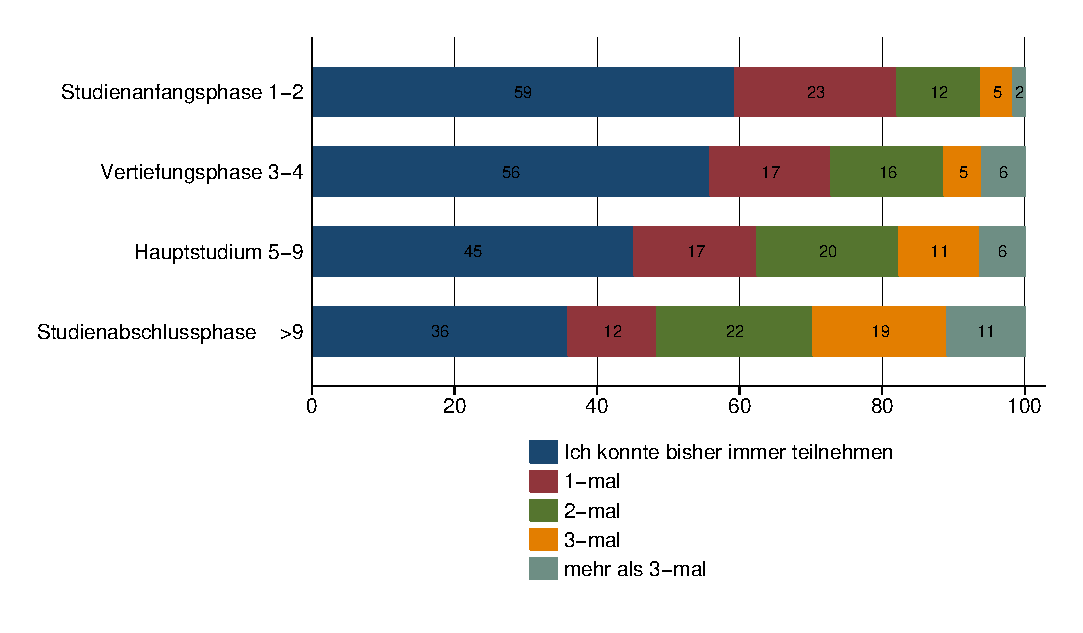
\includegraphics[RemoveGraphicsExtensions={.pdf,PDF}]{image}|
% \end{quote}
%
% \subsection{\plainTeX}
%
% \LaTeX's graphics packages can also be used with \plainTeX.
% The necessary basic \LaTeX\ macros are defined in
% \xfile{miniltx.tex}. This package \xpackage{grfext} also
% relies on it. Example:
%\begin{quote}
%\begin{verbatim}
%\input miniltx.tex\relax
%\def\Gin@driver{pdftex.def}
%\input graphicx.sty\relax
%\input grfext.sty\relax
%\resetatcatcode
%\end{verbatim}
%\end{quote}
%
% \StopEventually{
% }
%
% \section{Implementation}
%
%    \begin{macrocode}
%<*package>
%    \end{macrocode}
%
% \subsection{Relead check and identification}
%    Reload check, especially if the package is not used with \LaTeX.
%    \begin{macrocode}
\begingroup\catcode61\catcode48\catcode32=10\relax%
  \catcode13=5 % ^^M
  \endlinechar=13 %
  \catcode35=6 % #
  \catcode39=12 % '
  \catcode44=12 % ,
  \catcode45=12 % -
  \catcode46=12 % .
  \catcode58=12 % :
  \catcode64=11 % @
  \catcode123=1 % {
  \catcode125=2 % }
  \expandafter\let\expandafter\x\csname ver@grfext.sty\endcsname
  \ifx\x\relax % plain-TeX, first loading
  \else
    \def\empty{}%
    \ifx\x\empty % LaTeX, first loading,
      % variable is initialized, but \ProvidesPackage not yet seen
    \else
      \expandafter\ifx\csname PackageInfo\endcsname\relax
        \def\x#1#2{%
          \immediate\write-1{Package #1 Info: #2.}%
        }%
      \else
        \def\x#1#2{\PackageInfo{#1}{#2, stopped}}%
      \fi
      \x{grfext}{The package is already loaded}%
      \aftergroup\endinput
    \fi
  \fi
\endgroup%
%    \end{macrocode}
%    Package identification:
%    \begin{macrocode}
\begingroup\catcode61\catcode48\catcode32=10\relax%
  \catcode13=5 % ^^M
  \endlinechar=13 %
  \catcode35=6 % #
  \catcode39=12 % '
  \catcode40=12 % (
  \catcode41=12 % )
  \catcode44=12 % ,
  \catcode45=12 % -
  \catcode46=12 % .
  \catcode47=12 % /
  \catcode58=12 % :
  \catcode64=11 % @
  \catcode91=12 % [
  \catcode93=12 % ]
  \catcode123=1 % {
  \catcode125=2 % }
  \expandafter\ifx\csname ProvidesPackage\endcsname\relax
    \def\x#1#2#3[#4]{\endgroup
      \immediate\write-1{Package: #3 #4}%
      \xdef#1{#4}%
    }%
  \else
    \def\x#1#2[#3]{\endgroup
      #2[{#3}]%
      \ifx#1\@undefined
        \xdef#1{#3}%
      \fi
      \ifx#1\relax
        \xdef#1{#3}%
      \fi
    }%
  \fi
\expandafter\x\csname ver@grfext.sty\endcsname
\ProvidesPackage{grfext}%
  [2019/12/03 v1.3 Manage graphics extensions (HO)]%
%    \end{macrocode}
%
% \subsection{Catcodes}
%
%    \begin{macrocode}
\begingroup\catcode61\catcode48\catcode32=10\relax%
  \catcode13=5 % ^^M
  \endlinechar=13 %
  \catcode123=1 % {
  \catcode125=2 % }
  \catcode64=11 % @
  \def\x{\endgroup
    \expandafter\edef\csname grfext@AtEnd\endcsname{%
      \endlinechar=\the\endlinechar\relax
      \catcode13=\the\catcode13\relax
      \catcode32=\the\catcode32\relax
      \catcode35=\the\catcode35\relax
      \catcode61=\the\catcode61\relax
      \catcode64=\the\catcode64\relax
      \catcode123=\the\catcode123\relax
      \catcode125=\the\catcode125\relax
    }%
  }%
\x\catcode61\catcode48\catcode32=10\relax%
\catcode13=5 % ^^M
\endlinechar=13 %
\catcode35=6 % #
\catcode64=11 % @
\catcode123=1 % {
\catcode125=2 % }
\def\TMP@EnsureCode#1#2{%
  \edef\grfext@AtEnd{%
    \grfext@AtEnd
    \catcode#1=\the\catcode#1\relax
  }%
  \catcode#1=#2\relax
}
\TMP@EnsureCode{42}{12}% *
\TMP@EnsureCode{44}{12}% ,
\TMP@EnsureCode{47}{12}% /
\TMP@EnsureCode{58}{12}% :
\TMP@EnsureCode{60}{12}% <
\TMP@EnsureCode{62}{12}% >
\TMP@EnsureCode{91}{12}% [
\TMP@EnsureCode{93}{12}% ]
\edef\grfext@AtEnd{\grfext@AtEnd\noexpand\endinput}
%    \end{macrocode}
%
% \subsection{\plainTeX}
%
%    \begin{macro}{\@expandtwoargs}
%    Requirement is \xfile{miniltx.tex}, but we need also
%    \LaTeX's \cs{@expandtwoargs}.
%    \begin{macrocode}
\@ifundefined{@expandtwoargs}{%
  \def\@expandtwoargs#1#2#3{%
    \edef\reserved@a{\noexpand#1{#2}{#3}}%
    \reserved@a
  }%
}{}
%    \end{macrocode}
%    \end{macro}
%
% \subsection{Add}
%
%    \begin{macro}{\AppendGraphicsExtensions}
%    \begin{macrocode}
\newcommand*{\AppendGraphicsExtensions}{%
  \@ifundefined{Gin@extensions}{%
    \let\Gin@extensions\@empty
  }{}%
  \@ifstar{\grfext@Append\grfext@Check}{\grfext@Append\grfext@@Add}%
}%
%    \end{macrocode}
%    \end{macro}
%    \begin{macro}{\grfext@Append}
%    \begin{macrocode}
\def\grfext@Append#1#2{%
  \let\grfext@Print\@gobble
  \edef\grfext@next{%
    \noexpand\grfext@Add\noexpand#1{%
      \zap@space#2 \@empty
    }{\noexpand\Gin@extensions,}{}%
  }%
  \grfext@next
  \let\grfext@Print\grfext@@Print
  \grfext@Print\AppendGraphicsExtensions
}
%    \end{macrocode}
%    \end{macro}
%
%    \begin{macro}{\PrependGraphicsExtensions}
%    \begin{macrocode}
\newcommand*{\PrependGraphicsExtensions}{%
  \@ifundefined{Gin@extensions}{%
    \let\Gin@extensions\@empty
  }{}%
  \@ifstar{\grfext@Prepend\grfext@Check}{\grfext@Prepend\grfext@@Add}%
}%
%    \end{macrocode}
%    \end{macro}
%    \begin{macro}{\grfext@Prepend}
%    \begin{macrocode}
\def\grfext@Prepend#1#2{%
  \let\grfext@Print\@gobble
  \edef\grfext@next{%
    \noexpand\grfext@Add\noexpand#1{%
      \zap@space#2 \@empty
    }{}{,\noexpand\Gin@extensions}%
  }%
  \grfext@next
  \let\grfext@Print\grfext@@Print
  \grfext@Print\PrependGraphicsExtensions
}
%    \end{macrocode}
%    \end{macro}
%
%    \begin{macro}{\grfext@Add}
%    \begin{macrocode}
\def\grfext@Add#1#2{%
  #1{#2}%
}
%    \end{macrocode}
%    \end{macro}
%    \begin{macro}{\grfext@@Add}
%    \begin{macrocode}
\def\grfext@@Add#1#2#3{%
  \RemoveGraphicsExtensions{#1}%
  \ifx\Gin@extensions\@empty
    \def\Gin@extensions{#1}%
  \else
    \edef\Gin@extensions{#2#1#3}%
  \fi
}
%    \end{macrocode}
%    \end{macro}
%
% \subsection{Check}
%
%    \begin{macro}{\grfext@Check}
%    \begin{macrocode}
\def\grfext@Check#1{%
  \let\grfext@tmp\@empty
  \@for\grfext@ext:=#1\do{%
    \@ifundefined{Gin@rule@\grfext@ext}{%
    }{%
      \ifx\grfext@tmp\@empty
        \let\grfext@tmp\grfext@ext
      \else
        \edef\grfext@tmp{\grfext@tmp,\grfext@ext}%
      \fi
    }%
  }%
  \ifx\grfext@tmp\@empty
    \def\grfext@next##1##2{}%
  \else
    \edef\grfext@next{%
      \noexpand\grfext@@Add{\grfext@tmp}%
    }%
  \fi
  \grfext@next
}
%    \end{macrocode}
%    \end{macro}
%
% \subsection{Remove}
%
%    \begin{macro}{\RemoveGraphicsExtensions}
%    \begin{macrocode}
\newcommand*{\RemoveGraphicsExtensions}[1]{%
  \@ifundefined{Gin@extensions}{%
    \def\Gin@extensions{}%
  }{%
    \edef\grfext@tmp{\zap@space#1 \@empty}%
    \@for\grfext@ext:=\grfext@tmp\do{%
      \def\grfext@next{%
        \let\grfext@tmp\Gin@extensions
        \@expandtwoargs
        \@removeelement\grfext@ext\Gin@extensions\Gin@extensions
        \ifx\grfext@tmp\Gin@extensions
          \let\grfext@next\relax
        \fi
        \grfext@next
      }%
      \grfext@next
    }%
  }%
  \grfext@Print\RemoveGraphicsExtensions
}
%    \end{macrocode}
%    \end{macro}
%
% \subsection{Print}
%
%    \begin{macrocode}
\RequirePackage{infwarerr}[2007/09/09]
%    \end{macrocode}
%
%    \begin{macro}{\PrintGraphicsExtensions}
%    \begin{macrocode}
\def\PrintGraphicsExtensions{%
  \grfext@Print\PrintGraphicsExtensions
}
%    \end{macrocode}
%    \end{macro}
%    \begin{macro}{\grfext@Print}
%    \begin{macrocode}
\def\grfext@Print#1{%
  \@PackageInfo{grfext}{%
    Graphics extension search list:\MessageBreak
    \@ifundefined{Gin@extensions}{%
      <unavailable>%
    }{%
      [\Gin@extensions]%
    }\MessageBreak
    \string#1%
  }%
}
%    \end{macrocode}
%    \end{macro}
%    \begin{macro}{\grfext@@Print}
%    \begin{macrocode}
\let\grfext@@Print\grfext@Print
%    \end{macrocode}
%    \end{macro}
%
% \subsection{Defining options for package \xpackage{graphicx}}
%
%    \begin{macrocode}
\RequirePackage{kvdefinekeys}[2010/03/01]
\kv@define@key{Gin}{AppendGraphicsExtensions}{%
  \AppendGraphicsExtensions{#1}%
}
\kv@define@key{Gin}{AppendGraphicsExtensions*}{%
  \AppendGraphicsExtensions*{#1}%
}
\kv@define@key{Gin}{PrependGraphicsExtensions}{%
  \PrependGraphicsExtensions{#1}%
}
\kv@define@key{Gin}{PrependGraphicsExtensions*}{%
  \PrependGraphicsExtensions*{#1}%
}
\kv@define@key{Gin}{RemoveGraphicsExtensions}{%
  \RemoveGraphicsExtensions{#1}%
}
\kv@define@key{Gin}{PrintGraphicsExtensions}[]{%
  \PrintGraphicsExtensions
}
%    \end{macrocode}
%
%    \begin{macrocode}
\grfext@AtEnd%
%</package>
%    \end{macrocode}
% \section{Installation}
%
% \subsection{Download}
%
% \paragraph{Package.} This package is available on
% CTAN\footnote{\CTANpkg{grfext}}:
% \begin{description}
% \item[\CTAN{macros/latex/contrib/grfext/grfext.dtx}] The source file.
% \item[\CTAN{macros/latex/contrib/grfext/grfext.pdf}] Documentation.
% \end{description}
%
%
% \paragraph{Bundle.} All the packages of the bundle `grfext'
% are also available in a TDS compliant ZIP archive. There
% the packages are already unpacked and the documentation files
% are generated. The files and directories obey the TDS standard.
% \begin{description}
% \item[\CTANinstall{install/macros/latex/contrib/grfext.tds.zip}]
% \end{description}
% \emph{TDS} refers to the standard ``A Directory Structure
% for \TeX\ Files'' (\CTANpkg{tds}). Directories
% with \xfile{texmf} in their name are usually organized this way.
%
% \subsection{Bundle installation}
%
% \paragraph{Unpacking.} Unpack the \xfile{grfext.tds.zip} in the
% TDS tree (also known as \xfile{texmf} tree) of your choice.
% Example (linux):
% \begin{quote}
%   |unzip grfext.tds.zip -d ~/texmf|
% \end{quote}
%
% \subsection{Package installation}
%
% \paragraph{Unpacking.} The \xfile{.dtx} file is a self-extracting
% \docstrip\ archive. The files are extracted by running the
% \xfile{.dtx} through \plainTeX:
% \begin{quote}
%   \verb|tex grfext.dtx|
% \end{quote}
%
% \paragraph{TDS.} Now the different files must be moved into
% the different directories in your installation TDS tree
% (also known as \xfile{texmf} tree):
% \begin{quote}
% \def\t{^^A
% \begin{tabular}{@{}>{\ttfamily}l@{ $\rightarrow$ }>{\ttfamily}l@{}}
%   grfext.sty & tex/latex/grfext/grfext.sty\\
%   grfext.pdf & doc/latex/grfext/grfext.pdf\\
%   grfext.dtx & source/latex/grfext/grfext.dtx\\
% \end{tabular}^^A
% }^^A
% \sbox0{\t}^^A
% \ifdim\wd0>\linewidth
%   \begingroup
%     \advance\linewidth by\leftmargin
%     \advance\linewidth by\rightmargin
%   \edef\x{\endgroup
%     \def\noexpand\lw{\the\linewidth}^^A
%   }\x
%   \def\lwbox{^^A
%     \leavevmode
%     \hbox to \linewidth{^^A
%       \kern-\leftmargin\relax
%       \hss
%       \usebox0
%       \hss
%       \kern-\rightmargin\relax
%     }^^A
%   }^^A
%   \ifdim\wd0>\lw
%     \sbox0{\small\t}^^A
%     \ifdim\wd0>\linewidth
%       \ifdim\wd0>\lw
%         \sbox0{\footnotesize\t}^^A
%         \ifdim\wd0>\linewidth
%           \ifdim\wd0>\lw
%             \sbox0{\scriptsize\t}^^A
%             \ifdim\wd0>\linewidth
%               \ifdim\wd0>\lw
%                 \sbox0{\tiny\t}^^A
%                 \ifdim\wd0>\linewidth
%                   \lwbox
%                 \else
%                   \usebox0
%                 \fi
%               \else
%                 \lwbox
%               \fi
%             \else
%               \usebox0
%             \fi
%           \else
%             \lwbox
%           \fi
%         \else
%           \usebox0
%         \fi
%       \else
%         \lwbox
%       \fi
%     \else
%       \usebox0
%     \fi
%   \else
%     \lwbox
%   \fi
% \else
%   \usebox0
% \fi
% \end{quote}
% If you have a \xfile{docstrip.cfg} that configures and enables \docstrip's
% TDS installing feature, then some files can already be in the right
% place, see the documentation of \docstrip.
%
% \subsection{Refresh file name databases}
%
% If your \TeX~distribution
% (\TeX\,Live, \mikTeX, \dots) relies on file name databases, you must refresh
% these. For example, \TeX\,Live\ users run \verb|texhash| or
% \verb|mktexlsr|.
%
% \subsection{Some details for the interested}
%
% \paragraph{Unpacking with \LaTeX.}
% The \xfile{.dtx} chooses its action depending on the format:
% \begin{description}
% \item[\plainTeX:] Run \docstrip\ and extract the files.
% \item[\LaTeX:] Generate the documentation.
% \end{description}
% If you insist on using \LaTeX\ for \docstrip\ (really,
% \docstrip\ does not need \LaTeX), then inform the autodetect routine
% about your intention:
% \begin{quote}
%   \verb|latex \let\install=y\input{grfext.dtx}|
% \end{quote}
% Do not forget to quote the argument according to the demands
% of your shell.
%
% \paragraph{Generating the documentation.}
% You can use both the \xfile{.dtx} or the \xfile{.drv} to generate
% the documentation. The process can be configured by the
% configuration file \xfile{ltxdoc.cfg}. For instance, put this
% line into this file, if you want to have A4 as paper format:
% \begin{quote}
%   \verb|\PassOptionsToClass{a4paper}{article}|
% \end{quote}
% An example follows how to generate the
% documentation with pdf\LaTeX:
% \begin{quote}
%\begin{verbatim}
%pdflatex grfext.dtx
%makeindex -s gind.ist grfext.idx
%pdflatex grfext.dtx
%makeindex -s gind.ist grfext.idx
%pdflatex grfext.dtx
%\end{verbatim}
% \end{quote}
%
% \begin{thebibliography}{9}
%
% \bibitem{graphics}
%   David Carlisle, Sebastian Rahtz: \textit{The \xpackage{graphics} package};
%   2006/02/20 v1.0o;
%   \CTAN{macros/latex/required/graphics/graphics.dtx}.
%
% \end{thebibliography}
%
% \begin{History}
%   \begin{Version}{2007/09/30 v1.0}
%   \item
%     First public version.
%   \end{Version}
%   \begin{Version}{2010/08/19 v1.1}
%   \item
%     User macros are also made available as keyval options for
%     package \xpackage{graphicx}.
%   \end{Version}
%   \begin{Version}{2016/05/16 v1.2}
%   \item
%     Documentation updates.
%   \end{Version}
%   \begin{Version}{2019/12/03 v1.3}
%   \item
%     Documentation updates.
%   \end{Version}
% \end{History}
%
% \PrintIndex
%
% \Finale
\endinput
|
% \end{quote}
% Do not forget to quote the argument according to the demands
% of your shell.
%
% \paragraph{Generating the documentation.}
% You can use both the \xfile{.dtx} or the \xfile{.drv} to generate
% the documentation. The process can be configured by the
% configuration file \xfile{ltxdoc.cfg}. For instance, put this
% line into this file, if you want to have A4 as paper format:
% \begin{quote}
%   \verb|\PassOptionsToClass{a4paper}{article}|
% \end{quote}
% An example follows how to generate the
% documentation with pdf\LaTeX:
% \begin{quote}
%\begin{verbatim}
%pdflatex grfext.dtx
%makeindex -s gind.ist grfext.idx
%pdflatex grfext.dtx
%makeindex -s gind.ist grfext.idx
%pdflatex grfext.dtx
%\end{verbatim}
% \end{quote}
%
% \begin{thebibliography}{9}
%
% \bibitem{graphics}
%   David Carlisle, Sebastian Rahtz: \textit{The \xpackage{graphics} package};
%   2006/02/20 v1.0o;
%   \CTAN{macros/latex/required/graphics/graphics.dtx}.
%
% \end{thebibliography}
%
% \begin{History}
%   \begin{Version}{2007/09/30 v1.0}
%   \item
%     First public version.
%   \end{Version}
%   \begin{Version}{2010/08/19 v1.1}
%   \item
%     User macros are also made available as keyval options for
%     package \xpackage{graphicx}.
%   \end{Version}
%   \begin{Version}{2016/05/16 v1.2}
%   \item
%     Documentation updates.
%   \end{Version}
%   \begin{Version}{2019/12/03 v1.3}
%   \item
%     Documentation updates.
%   \end{Version}
% \end{History}
%
% \PrintIndex
%
% \Finale
\endinput
|
% \end{quote}
% Do not forget to quote the argument according to the demands
% of your shell.
%
% \paragraph{Generating the documentation.}
% You can use both the \xfile{.dtx} or the \xfile{.drv} to generate
% the documentation. The process can be configured by the
% configuration file \xfile{ltxdoc.cfg}. For instance, put this
% line into this file, if you want to have A4 as paper format:
% \begin{quote}
%   \verb|\PassOptionsToClass{a4paper}{article}|
% \end{quote}
% An example follows how to generate the
% documentation with pdf\LaTeX:
% \begin{quote}
%\begin{verbatim}
%pdflatex grfext.dtx
%makeindex -s gind.ist grfext.idx
%pdflatex grfext.dtx
%makeindex -s gind.ist grfext.idx
%pdflatex grfext.dtx
%\end{verbatim}
% \end{quote}
%
% \begin{thebibliography}{9}
%
% \bibitem{graphics}
%   David Carlisle, Sebastian Rahtz: \textit{The \xpackage{graphics} package};
%   2006/02/20 v1.0o;
%   \CTAN{macros/latex/required/graphics/graphics.dtx}.
%
% \end{thebibliography}
%
% \begin{History}
%   \begin{Version}{2007/09/30 v1.0}
%   \item
%     First public version.
%   \end{Version}
%   \begin{Version}{2010/08/19 v1.1}
%   \item
%     User macros are also made available as keyval options for
%     package \xpackage{graphicx}.
%   \end{Version}
%   \begin{Version}{2016/05/16 v1.2}
%   \item
%     Documentation updates.
%   \end{Version}
%   \begin{Version}{2019/12/03 v1.3}
%   \item
%     Documentation updates.
%   \end{Version}
% \end{History}
%
% \PrintIndex
%
% \Finale
\endinput

%        (quote the arguments according to the demands of your shell)
%
% Documentation:
%    (a) If grfext.drv is present:
%           latex grfext.drv
%    (b) Without grfext.drv:
%           latex grfext.dtx; ...
%    The class ltxdoc loads the configuration file ltxdoc.cfg
%    if available. Here you can specify further options, e.g.
%    use A4 as paper format:
%       \PassOptionsToClass{a4paper}{article}
%
%    Programm calls to get the documentation (example):
%       pdflatex grfext.dtx
%       makeindex -s gind.ist grfext.idx
%       pdflatex grfext.dtx
%       makeindex -s gind.ist grfext.idx
%       pdflatex grfext.dtx
%
% Installation:
%    TDS:tex/latex/grfext/grfext.sty
%    TDS:doc/latex/grfext/grfext.pdf
%    TDS:source/latex/grfext/grfext.dtx
%
%<*ignore>
\begingroup
  \catcode123=1 %
  \catcode125=2 %
  \def\x{LaTeX2e}%
\expandafter\endgroup
\ifcase 0\ifx\install y1\fi\expandafter
         \ifx\csname processbatchFile\endcsname\relax\else1\fi
         \ifx\fmtname\x\else 1\fi\relax
\else\csname fi\endcsname
%</ignore>
%<*install>
\input docstrip.tex
\Msg{************************************************************************}
\Msg{* Installation}
\Msg{* Package: grfext 2019/12/03 v1.3 Manage graphics extensions (HO)}
\Msg{************************************************************************}

\keepsilent
\askforoverwritefalse

\let\MetaPrefix\relax
\preamble

This is a generated file.

Project: grfext
Version: 2019/12/03 v1.3

Copyright (C)
   2007, 2010 Heiko Oberdiek
   2016-2019 Oberdiek Package Support Group

This work may be distributed and/or modified under the
conditions of the LaTeX Project Public License, either
version 1.3c of this license or (at your option) any later
version. This version of this license is in
   https://www.latex-project.org/lppl/lppl-1-3c.txt
and the latest version of this license is in
   https://www.latex-project.org/lppl.txt
and version 1.3 or later is part of all distributions of
LaTeX version 2005/12/01 or later.

This work has the LPPL maintenance status "maintained".

The Current Maintainers of this work are
Heiko Oberdiek and the Oberdiek Package Support Group
https://github.com/ho-tex/grfext/issues


This work consists of the main source file grfext.dtx
and the derived files
   grfext.sty, grfext.pdf, grfext.ins, grfext.drv.

\endpreamble
\let\MetaPrefix\DoubleperCent

\generate{%
  \file{grfext.ins}{\from{grfext.dtx}{install}}%
  \file{grfext.drv}{\from{grfext.dtx}{driver}}%
  \usedir{tex/latex/grfext}%
  \file{grfext.sty}{\from{grfext.dtx}{package}}%
%  \usedir{doc/latex/grfext/test}%
%  \file{grfext-test1.tex}{\from{grfext.dtx}{test1}}%
%  \file{grfext-test2.tex}{\from{grfext.dtx}{test2}}%
}

\catcode32=13\relax% active space
\let =\space%
\Msg{************************************************************************}
\Msg{*}
\Msg{* To finish the installation you have to move the following}
\Msg{* file into a directory searched by TeX:}
\Msg{*}
\Msg{*     grfext.sty}
\Msg{*}
\Msg{* To produce the documentation run the file `grfext.drv'}
\Msg{* through LaTeX.}
\Msg{*}
\Msg{* Happy TeXing!}
\Msg{*}
\Msg{************************************************************************}

\endbatchfile
%</install>
%<*ignore>
\fi
%</ignore>
%<*driver>
\NeedsTeXFormat{LaTeX2e}
\ProvidesFile{grfext.drv}%
  [2019/12/03 v1.3 Manage graphics extensions (HO)]%
\documentclass{ltxdoc}
\usepackage{holtxdoc}[2011/11/22]
\begin{document}
  \DocInput{grfext.dtx}%
\end{document}
%</driver>
% \fi
%
%
%
% \GetFileInfo{grfext.drv}
%
% \title{The \xpackage{grfext} package}
% \date{2019/12/03 v1.3}
% \author{Heiko Oberdiek\thanks
% {Please report any issues at \url{https://github.com/ho-tex/grfext/issues}}}
%
% \maketitle
%
% \begin{abstract}
% This package provides macros for adding and reordering
% graphics extensions of package \xpackage{graphics}.
% \end{abstract}
%
% \tableofcontents
%
% \section{Documentation}
%
% \subsection{Introduction}
%
% If you are not familiar with \LaTeX's graphics bundle, please
% read its documentation \xfile{grffile} \cite{graphics}.
% The bundle contains two packages for graphics inclusion:
% \xpackage{graphics} and \xpackage{graphicx}. The first one
% is loaded by the second one that adds a key value interface.
%
% Graphics files are included in both cases by macro
% \cs{includegraphics}. The file name extension can be omitted.
% Then the graphics package goes through a list of known
% extensions until it finds the graphics file. This extension list
% is set by \cs{DeclareGraphicsExtensions}. The previous contents
% of the list is overwritten.
%
% \subsection{User interface}
%
% This package \xpackage{grfext} provides macros that adds entries
% to the list or remove them. The list may be empty or even
% undefined before. It is always defined afterwards, but can
% be empty (especially after removing entries).
%
% \begin{declcs}{AppendGraphicsExtensions} * \M{ext-list}\\
%   \cs{PrependGraphicsExtensions} * \M{ext-list}
% \end{declcs}
% The argument \meta{ext-list} is a comma separated list whose
% entries are file name extensions including the dot.
% But first the entries are removed from
% \xpackage{graphics}' extension list to avoid multiple
% occurences of the same extension.
%
% Then macro \cs{AppendGraphicsExtensions} adds the entries
% after the end of \xpackage{graphics}' list, whereas
% macro \cs{PrependGraphicsExtensions} puts them in front
% of the list.
% The order matters if a graphics file is available in
% different acceptable formats. Then the first extension
% wins.
%
% The star version of these commands only adds an extensions,
% if a specific graphics rule exists for that extension.
%
% \begin{declcs}{RemoveGraphicsExtensions} \M{ext-list}
% \end{declcs}
% All occurences of file extensions in \meta{ext-list} are
% removed from \xpackage{graphics}' extension list.
%
% \subsection{Package loading}
%
% The package does not define any options. It is loaded
% as usual in \LaTeX, e.g.:
% \begin{quote}
%   |\usepackage{grfext}|
% \end{quote}
%
% \begin{declcs}{PrintGraphicsExtensions}
% \end{declcs}
% Macro \cs{PrintGraphicsExtensions} writes the current
% graphics extensions list in the \xfile{.log} file.
% The macros described before do this automatically
% after their operation.
%
% \subsection{Option support for package \xpackage{graphicx}}
%
% Package \xpackage{graphicx} uses the interface of package
% \xpackage{keyval} in order to specify options for
% \cs{includegraphics}. The options can also be set using
% \begin{quote}
%   |\setkeys{Gin}{|\meta{options}|}|
% \end{quote}
% The four user macros with the two star forms are available
% as options in family |Gin| as well:
% \begin{quote}
%   |AppendGraphicsExtensions={|\meta{ext-list}|}|\\
%   |AppendGraphicsExtensions*={|\meta{ext-list}|}|\\
%   |PrependGraphicsExtensions={|\meta{ext-list}|}|\\
%   |PrependGraphicsExtensions*{|\meta{ext-list}|}|\\
%   |RemoveGraphicsExtensions={|\meta{ext-list}|}|\\
%   |PrintGraphicsExtensions|
% \end{quote}
% This makes it easier to locally change the extension list
% for an included graphics, e.g.:
% \begin{quote}
%   |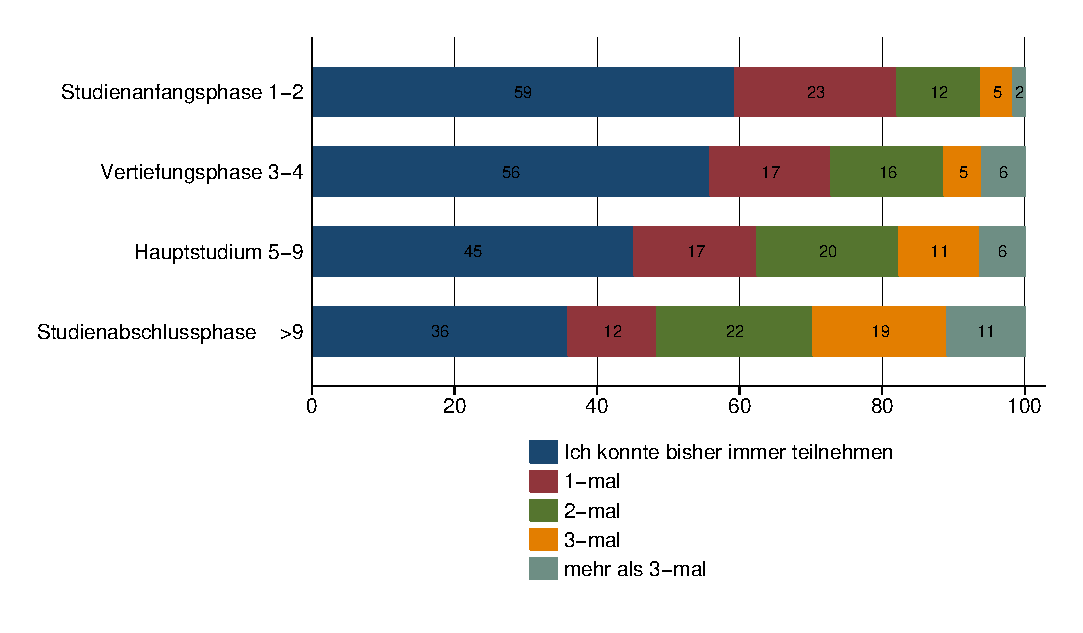
\includegraphics[RemoveGraphicsExtensions={.pdf,PDF}]{image}|
% \end{quote}
%
% \subsection{\plainTeX}
%
% \LaTeX's graphics packages can also be used with \plainTeX.
% The necessary basic \LaTeX\ macros are defined in
% \xfile{miniltx.tex}. This package \xpackage{grfext} also
% relies on it. Example:
%\begin{quote}
%\begin{verbatim}
%\input miniltx.tex\relax
%\def\Gin@driver{pdftex.def}
%\input graphicx.sty\relax
%\input grfext.sty\relax
%\resetatcatcode
%\end{verbatim}
%\end{quote}
%
% \StopEventually{
% }
%
% \section{Implementation}
%
%    \begin{macrocode}
%<*package>
%    \end{macrocode}
%
% \subsection{Relead check and identification}
%    Reload check, especially if the package is not used with \LaTeX.
%    \begin{macrocode}
\begingroup\catcode61\catcode48\catcode32=10\relax%
  \catcode13=5 % ^^M
  \endlinechar=13 %
  \catcode35=6 % #
  \catcode39=12 % '
  \catcode44=12 % ,
  \catcode45=12 % -
  \catcode46=12 % .
  \catcode58=12 % :
  \catcode64=11 % @
  \catcode123=1 % {
  \catcode125=2 % }
  \expandafter\let\expandafter\x\csname ver@grfext.sty\endcsname
  \ifx\x\relax % plain-TeX, first loading
  \else
    \def\empty{}%
    \ifx\x\empty % LaTeX, first loading,
      % variable is initialized, but \ProvidesPackage not yet seen
    \else
      \expandafter\ifx\csname PackageInfo\endcsname\relax
        \def\x#1#2{%
          \immediate\write-1{Package #1 Info: #2.}%
        }%
      \else
        \def\x#1#2{\PackageInfo{#1}{#2, stopped}}%
      \fi
      \x{grfext}{The package is already loaded}%
      \aftergroup\endinput
    \fi
  \fi
\endgroup%
%    \end{macrocode}
%    Package identification:
%    \begin{macrocode}
\begingroup\catcode61\catcode48\catcode32=10\relax%
  \catcode13=5 % ^^M
  \endlinechar=13 %
  \catcode35=6 % #
  \catcode39=12 % '
  \catcode40=12 % (
  \catcode41=12 % )
  \catcode44=12 % ,
  \catcode45=12 % -
  \catcode46=12 % .
  \catcode47=12 % /
  \catcode58=12 % :
  \catcode64=11 % @
  \catcode91=12 % [
  \catcode93=12 % ]
  \catcode123=1 % {
  \catcode125=2 % }
  \expandafter\ifx\csname ProvidesPackage\endcsname\relax
    \def\x#1#2#3[#4]{\endgroup
      \immediate\write-1{Package: #3 #4}%
      \xdef#1{#4}%
    }%
  \else
    \def\x#1#2[#3]{\endgroup
      #2[{#3}]%
      \ifx#1\@undefined
        \xdef#1{#3}%
      \fi
      \ifx#1\relax
        \xdef#1{#3}%
      \fi
    }%
  \fi
\expandafter\x\csname ver@grfext.sty\endcsname
\ProvidesPackage{grfext}%
  [2019/12/03 v1.3 Manage graphics extensions (HO)]%
%    \end{macrocode}
%
% \subsection{Catcodes}
%
%    \begin{macrocode}
\begingroup\catcode61\catcode48\catcode32=10\relax%
  \catcode13=5 % ^^M
  \endlinechar=13 %
  \catcode123=1 % {
  \catcode125=2 % }
  \catcode64=11 % @
  \def\x{\endgroup
    \expandafter\edef\csname grfext@AtEnd\endcsname{%
      \endlinechar=\the\endlinechar\relax
      \catcode13=\the\catcode13\relax
      \catcode32=\the\catcode32\relax
      \catcode35=\the\catcode35\relax
      \catcode61=\the\catcode61\relax
      \catcode64=\the\catcode64\relax
      \catcode123=\the\catcode123\relax
      \catcode125=\the\catcode125\relax
    }%
  }%
\x\catcode61\catcode48\catcode32=10\relax%
\catcode13=5 % ^^M
\endlinechar=13 %
\catcode35=6 % #
\catcode64=11 % @
\catcode123=1 % {
\catcode125=2 % }
\def\TMP@EnsureCode#1#2{%
  \edef\grfext@AtEnd{%
    \grfext@AtEnd
    \catcode#1=\the\catcode#1\relax
  }%
  \catcode#1=#2\relax
}
\TMP@EnsureCode{42}{12}% *
\TMP@EnsureCode{44}{12}% ,
\TMP@EnsureCode{47}{12}% /
\TMP@EnsureCode{58}{12}% :
\TMP@EnsureCode{60}{12}% <
\TMP@EnsureCode{62}{12}% >
\TMP@EnsureCode{91}{12}% [
\TMP@EnsureCode{93}{12}% ]
\edef\grfext@AtEnd{\grfext@AtEnd\noexpand\endinput}
%    \end{macrocode}
%
% \subsection{\plainTeX}
%
%    \begin{macro}{\@expandtwoargs}
%    Requirement is \xfile{miniltx.tex}, but we need also
%    \LaTeX's \cs{@expandtwoargs}.
%    \begin{macrocode}
\@ifundefined{@expandtwoargs}{%
  \def\@expandtwoargs#1#2#3{%
    \edef\reserved@a{\noexpand#1{#2}{#3}}%
    \reserved@a
  }%
}{}
%    \end{macrocode}
%    \end{macro}
%
% \subsection{Add}
%
%    \begin{macro}{\AppendGraphicsExtensions}
%    \begin{macrocode}
\newcommand*{\AppendGraphicsExtensions}{%
  \@ifundefined{Gin@extensions}{%
    \let\Gin@extensions\@empty
  }{}%
  \@ifstar{\grfext@Append\grfext@Check}{\grfext@Append\grfext@@Add}%
}%
%    \end{macrocode}
%    \end{macro}
%    \begin{macro}{\grfext@Append}
%    \begin{macrocode}
\def\grfext@Append#1#2{%
  \let\grfext@Print\@gobble
  \edef\grfext@next{%
    \noexpand\grfext@Add\noexpand#1{%
      \zap@space#2 \@empty
    }{\noexpand\Gin@extensions,}{}%
  }%
  \grfext@next
  \let\grfext@Print\grfext@@Print
  \grfext@Print\AppendGraphicsExtensions
}
%    \end{macrocode}
%    \end{macro}
%
%    \begin{macro}{\PrependGraphicsExtensions}
%    \begin{macrocode}
\newcommand*{\PrependGraphicsExtensions}{%
  \@ifundefined{Gin@extensions}{%
    \let\Gin@extensions\@empty
  }{}%
  \@ifstar{\grfext@Prepend\grfext@Check}{\grfext@Prepend\grfext@@Add}%
}%
%    \end{macrocode}
%    \end{macro}
%    \begin{macro}{\grfext@Prepend}
%    \begin{macrocode}
\def\grfext@Prepend#1#2{%
  \let\grfext@Print\@gobble
  \edef\grfext@next{%
    \noexpand\grfext@Add\noexpand#1{%
      \zap@space#2 \@empty
    }{}{,\noexpand\Gin@extensions}%
  }%
  \grfext@next
  \let\grfext@Print\grfext@@Print
  \grfext@Print\PrependGraphicsExtensions
}
%    \end{macrocode}
%    \end{macro}
%
%    \begin{macro}{\grfext@Add}
%    \begin{macrocode}
\def\grfext@Add#1#2{%
  #1{#2}%
}
%    \end{macrocode}
%    \end{macro}
%    \begin{macro}{\grfext@@Add}
%    \begin{macrocode}
\def\grfext@@Add#1#2#3{%
  \RemoveGraphicsExtensions{#1}%
  \ifx\Gin@extensions\@empty
    \def\Gin@extensions{#1}%
  \else
    \edef\Gin@extensions{#2#1#3}%
  \fi
}
%    \end{macrocode}
%    \end{macro}
%
% \subsection{Check}
%
%    \begin{macro}{\grfext@Check}
%    \begin{macrocode}
\def\grfext@Check#1{%
  \let\grfext@tmp\@empty
  \@for\grfext@ext:=#1\do{%
    \@ifundefined{Gin@rule@\grfext@ext}{%
    }{%
      \ifx\grfext@tmp\@empty
        \let\grfext@tmp\grfext@ext
      \else
        \edef\grfext@tmp{\grfext@tmp,\grfext@ext}%
      \fi
    }%
  }%
  \ifx\grfext@tmp\@empty
    \def\grfext@next##1##2{}%
  \else
    \edef\grfext@next{%
      \noexpand\grfext@@Add{\grfext@tmp}%
    }%
  \fi
  \grfext@next
}
%    \end{macrocode}
%    \end{macro}
%
% \subsection{Remove}
%
%    \begin{macro}{\RemoveGraphicsExtensions}
%    \begin{macrocode}
\newcommand*{\RemoveGraphicsExtensions}[1]{%
  \@ifundefined{Gin@extensions}{%
    \def\Gin@extensions{}%
  }{%
    \edef\grfext@tmp{\zap@space#1 \@empty}%
    \@for\grfext@ext:=\grfext@tmp\do{%
      \def\grfext@next{%
        \let\grfext@tmp\Gin@extensions
        \@expandtwoargs
        \@removeelement\grfext@ext\Gin@extensions\Gin@extensions
        \ifx\grfext@tmp\Gin@extensions
          \let\grfext@next\relax
        \fi
        \grfext@next
      }%
      \grfext@next
    }%
  }%
  \grfext@Print\RemoveGraphicsExtensions
}
%    \end{macrocode}
%    \end{macro}
%
% \subsection{Print}
%
%    \begin{macrocode}
\RequirePackage{infwarerr}[2007/09/09]
%    \end{macrocode}
%
%    \begin{macro}{\PrintGraphicsExtensions}
%    \begin{macrocode}
\def\PrintGraphicsExtensions{%
  \grfext@Print\PrintGraphicsExtensions
}
%    \end{macrocode}
%    \end{macro}
%    \begin{macro}{\grfext@Print}
%    \begin{macrocode}
\def\grfext@Print#1{%
  \@PackageInfo{grfext}{%
    Graphics extension search list:\MessageBreak
    \@ifundefined{Gin@extensions}{%
      <unavailable>%
    }{%
      [\Gin@extensions]%
    }\MessageBreak
    \string#1%
  }%
}
%    \end{macrocode}
%    \end{macro}
%    \begin{macro}{\grfext@@Print}
%    \begin{macrocode}
\let\grfext@@Print\grfext@Print
%    \end{macrocode}
%    \end{macro}
%
% \subsection{Defining options for package \xpackage{graphicx}}
%
%    \begin{macrocode}
\RequirePackage{kvdefinekeys}[2010/03/01]
\kv@define@key{Gin}{AppendGraphicsExtensions}{%
  \AppendGraphicsExtensions{#1}%
}
\kv@define@key{Gin}{AppendGraphicsExtensions*}{%
  \AppendGraphicsExtensions*{#1}%
}
\kv@define@key{Gin}{PrependGraphicsExtensions}{%
  \PrependGraphicsExtensions{#1}%
}
\kv@define@key{Gin}{PrependGraphicsExtensions*}{%
  \PrependGraphicsExtensions*{#1}%
}
\kv@define@key{Gin}{RemoveGraphicsExtensions}{%
  \RemoveGraphicsExtensions{#1}%
}
\kv@define@key{Gin}{PrintGraphicsExtensions}[]{%
  \PrintGraphicsExtensions
}
%    \end{macrocode}
%
%    \begin{macrocode}
\grfext@AtEnd%
%</package>
%    \end{macrocode}
% \section{Installation}
%
% \subsection{Download}
%
% \paragraph{Package.} This package is available on
% CTAN\footnote{\CTANpkg{grfext}}:
% \begin{description}
% \item[\CTAN{macros/latex/contrib/grfext/grfext.dtx}] The source file.
% \item[\CTAN{macros/latex/contrib/grfext/grfext.pdf}] Documentation.
% \end{description}
%
%
% \paragraph{Bundle.} All the packages of the bundle `grfext'
% are also available in a TDS compliant ZIP archive. There
% the packages are already unpacked and the documentation files
% are generated. The files and directories obey the TDS standard.
% \begin{description}
% \item[\CTANinstall{install/macros/latex/contrib/grfext.tds.zip}]
% \end{description}
% \emph{TDS} refers to the standard ``A Directory Structure
% for \TeX\ Files'' (\CTANpkg{tds}). Directories
% with \xfile{texmf} in their name are usually organized this way.
%
% \subsection{Bundle installation}
%
% \paragraph{Unpacking.} Unpack the \xfile{grfext.tds.zip} in the
% TDS tree (also known as \xfile{texmf} tree) of your choice.
% Example (linux):
% \begin{quote}
%   |unzip grfext.tds.zip -d ~/texmf|
% \end{quote}
%
% \subsection{Package installation}
%
% \paragraph{Unpacking.} The \xfile{.dtx} file is a self-extracting
% \docstrip\ archive. The files are extracted by running the
% \xfile{.dtx} through \plainTeX:
% \begin{quote}
%   \verb|tex grfext.dtx|
% \end{quote}
%
% \paragraph{TDS.} Now the different files must be moved into
% the different directories in your installation TDS tree
% (also known as \xfile{texmf} tree):
% \begin{quote}
% \def\t{^^A
% \begin{tabular}{@{}>{\ttfamily}l@{ $\rightarrow$ }>{\ttfamily}l@{}}
%   grfext.sty & tex/latex/grfext/grfext.sty\\
%   grfext.pdf & doc/latex/grfext/grfext.pdf\\
%   grfext.dtx & source/latex/grfext/grfext.dtx\\
% \end{tabular}^^A
% }^^A
% \sbox0{\t}^^A
% \ifdim\wd0>\linewidth
%   \begingroup
%     \advance\linewidth by\leftmargin
%     \advance\linewidth by\rightmargin
%   \edef\x{\endgroup
%     \def\noexpand\lw{\the\linewidth}^^A
%   }\x
%   \def\lwbox{^^A
%     \leavevmode
%     \hbox to \linewidth{^^A
%       \kern-\leftmargin\relax
%       \hss
%       \usebox0
%       \hss
%       \kern-\rightmargin\relax
%     }^^A
%   }^^A
%   \ifdim\wd0>\lw
%     \sbox0{\small\t}^^A
%     \ifdim\wd0>\linewidth
%       \ifdim\wd0>\lw
%         \sbox0{\footnotesize\t}^^A
%         \ifdim\wd0>\linewidth
%           \ifdim\wd0>\lw
%             \sbox0{\scriptsize\t}^^A
%             \ifdim\wd0>\linewidth
%               \ifdim\wd0>\lw
%                 \sbox0{\tiny\t}^^A
%                 \ifdim\wd0>\linewidth
%                   \lwbox
%                 \else
%                   \usebox0
%                 \fi
%               \else
%                 \lwbox
%               \fi
%             \else
%               \usebox0
%             \fi
%           \else
%             \lwbox
%           \fi
%         \else
%           \usebox0
%         \fi
%       \else
%         \lwbox
%       \fi
%     \else
%       \usebox0
%     \fi
%   \else
%     \lwbox
%   \fi
% \else
%   \usebox0
% \fi
% \end{quote}
% If you have a \xfile{docstrip.cfg} that configures and enables \docstrip's
% TDS installing feature, then some files can already be in the right
% place, see the documentation of \docstrip.
%
% \subsection{Refresh file name databases}
%
% If your \TeX~distribution
% (\TeX\,Live, \mikTeX, \dots) relies on file name databases, you must refresh
% these. For example, \TeX\,Live\ users run \verb|texhash| or
% \verb|mktexlsr|.
%
% \subsection{Some details for the interested}
%
% \paragraph{Unpacking with \LaTeX.}
% The \xfile{.dtx} chooses its action depending on the format:
% \begin{description}
% \item[\plainTeX:] Run \docstrip\ and extract the files.
% \item[\LaTeX:] Generate the documentation.
% \end{description}
% If you insist on using \LaTeX\ for \docstrip\ (really,
% \docstrip\ does not need \LaTeX), then inform the autodetect routine
% about your intention:
% \begin{quote}
%   \verb|latex \let\install=y% \iffalse meta-comment
%
% File: grfext.dtx
% Version: 2019/12/03 v1.3
% Info: Manage graphics extensions
%
% Copyright (C)
%    2007, 2010 Heiko Oberdiek
%    2016-2019 Oberdiek Package Support Group
%    https://github.com/ho-tex/grfext/issues
%
% This work may be distributed and/or modified under the
% conditions of the LaTeX Project Public License, either
% version 1.3c of this license or (at your option) any later
% version. This version of this license is in
%    https://www.latex-project.org/lppl/lppl-1-3c.txt
% and the latest version of this license is in
%    https://www.latex-project.org/lppl.txt
% and version 1.3 or later is part of all distributions of
% LaTeX version 2005/12/01 or later.
%
% This work has the LPPL maintenance status "maintained".
%
% The Current Maintainers of this work are
% Heiko Oberdiek and the Oberdiek Package Support Group
% https://github.com/ho-tex/grfext/issues
%
% This work consists of the main source file grfext.dtx
% and the derived files
%    grfext.sty, grfext.pdf, grfext.ins, grfext.drv,
%
% Distribution:
%    CTAN:macros/latex/contrib/grfext/grfext.dtx
%    CTAN:macros/latex/contrib/grfext/grfext.pdf
%
% Unpacking:
%    (a) If grfext.ins is present:
%           tex grfext.ins
%    (b) Without grfext.ins:
%           tex grfext.dtx
%    (c) If you insist on using LaTeX
%           latex \let\install=y% \iffalse meta-comment
%
% File: grfext.dtx
% Version: 2019/12/03 v1.3
% Info: Manage graphics extensions
%
% Copyright (C)
%    2007, 2010 Heiko Oberdiek
%    2016-2019 Oberdiek Package Support Group
%    https://github.com/ho-tex/grfext/issues
%
% This work may be distributed and/or modified under the
% conditions of the LaTeX Project Public License, either
% version 1.3c of this license or (at your option) any later
% version. This version of this license is in
%    https://www.latex-project.org/lppl/lppl-1-3c.txt
% and the latest version of this license is in
%    https://www.latex-project.org/lppl.txt
% and version 1.3 or later is part of all distributions of
% LaTeX version 2005/12/01 or later.
%
% This work has the LPPL maintenance status "maintained".
%
% The Current Maintainers of this work are
% Heiko Oberdiek and the Oberdiek Package Support Group
% https://github.com/ho-tex/grfext/issues
%
% This work consists of the main source file grfext.dtx
% and the derived files
%    grfext.sty, grfext.pdf, grfext.ins, grfext.drv,
%
% Distribution:
%    CTAN:macros/latex/contrib/grfext/grfext.dtx
%    CTAN:macros/latex/contrib/grfext/grfext.pdf
%
% Unpacking:
%    (a) If grfext.ins is present:
%           tex grfext.ins
%    (b) Without grfext.ins:
%           tex grfext.dtx
%    (c) If you insist on using LaTeX
%           latex \let\install=y% \iffalse meta-comment
%
% File: grfext.dtx
% Version: 2019/12/03 v1.3
% Info: Manage graphics extensions
%
% Copyright (C)
%    2007, 2010 Heiko Oberdiek
%    2016-2019 Oberdiek Package Support Group
%    https://github.com/ho-tex/grfext/issues
%
% This work may be distributed and/or modified under the
% conditions of the LaTeX Project Public License, either
% version 1.3c of this license or (at your option) any later
% version. This version of this license is in
%    https://www.latex-project.org/lppl/lppl-1-3c.txt
% and the latest version of this license is in
%    https://www.latex-project.org/lppl.txt
% and version 1.3 or later is part of all distributions of
% LaTeX version 2005/12/01 or later.
%
% This work has the LPPL maintenance status "maintained".
%
% The Current Maintainers of this work are
% Heiko Oberdiek and the Oberdiek Package Support Group
% https://github.com/ho-tex/grfext/issues
%
% This work consists of the main source file grfext.dtx
% and the derived files
%    grfext.sty, grfext.pdf, grfext.ins, grfext.drv,
%
% Distribution:
%    CTAN:macros/latex/contrib/grfext/grfext.dtx
%    CTAN:macros/latex/contrib/grfext/grfext.pdf
%
% Unpacking:
%    (a) If grfext.ins is present:
%           tex grfext.ins
%    (b) Without grfext.ins:
%           tex grfext.dtx
%    (c) If you insist on using LaTeX
%           latex \let\install=y\input{grfext.dtx}
%        (quote the arguments according to the demands of your shell)
%
% Documentation:
%    (a) If grfext.drv is present:
%           latex grfext.drv
%    (b) Without grfext.drv:
%           latex grfext.dtx; ...
%    The class ltxdoc loads the configuration file ltxdoc.cfg
%    if available. Here you can specify further options, e.g.
%    use A4 as paper format:
%       \PassOptionsToClass{a4paper}{article}
%
%    Programm calls to get the documentation (example):
%       pdflatex grfext.dtx
%       makeindex -s gind.ist grfext.idx
%       pdflatex grfext.dtx
%       makeindex -s gind.ist grfext.idx
%       pdflatex grfext.dtx
%
% Installation:
%    TDS:tex/latex/grfext/grfext.sty
%    TDS:doc/latex/grfext/grfext.pdf
%    TDS:source/latex/grfext/grfext.dtx
%
%<*ignore>
\begingroup
  \catcode123=1 %
  \catcode125=2 %
  \def\x{LaTeX2e}%
\expandafter\endgroup
\ifcase 0\ifx\install y1\fi\expandafter
         \ifx\csname processbatchFile\endcsname\relax\else1\fi
         \ifx\fmtname\x\else 1\fi\relax
\else\csname fi\endcsname
%</ignore>
%<*install>
\input docstrip.tex
\Msg{************************************************************************}
\Msg{* Installation}
\Msg{* Package: grfext 2019/12/03 v1.3 Manage graphics extensions (HO)}
\Msg{************************************************************************}

\keepsilent
\askforoverwritefalse

\let\MetaPrefix\relax
\preamble

This is a generated file.

Project: grfext
Version: 2019/12/03 v1.3

Copyright (C)
   2007, 2010 Heiko Oberdiek
   2016-2019 Oberdiek Package Support Group

This work may be distributed and/or modified under the
conditions of the LaTeX Project Public License, either
version 1.3c of this license or (at your option) any later
version. This version of this license is in
   https://www.latex-project.org/lppl/lppl-1-3c.txt
and the latest version of this license is in
   https://www.latex-project.org/lppl.txt
and version 1.3 or later is part of all distributions of
LaTeX version 2005/12/01 or later.

This work has the LPPL maintenance status "maintained".

The Current Maintainers of this work are
Heiko Oberdiek and the Oberdiek Package Support Group
https://github.com/ho-tex/grfext/issues


This work consists of the main source file grfext.dtx
and the derived files
   grfext.sty, grfext.pdf, grfext.ins, grfext.drv.

\endpreamble
\let\MetaPrefix\DoubleperCent

\generate{%
  \file{grfext.ins}{\from{grfext.dtx}{install}}%
  \file{grfext.drv}{\from{grfext.dtx}{driver}}%
  \usedir{tex/latex/grfext}%
  \file{grfext.sty}{\from{grfext.dtx}{package}}%
%  \usedir{doc/latex/grfext/test}%
%  \file{grfext-test1.tex}{\from{grfext.dtx}{test1}}%
%  \file{grfext-test2.tex}{\from{grfext.dtx}{test2}}%
}

\catcode32=13\relax% active space
\let =\space%
\Msg{************************************************************************}
\Msg{*}
\Msg{* To finish the installation you have to move the following}
\Msg{* file into a directory searched by TeX:}
\Msg{*}
\Msg{*     grfext.sty}
\Msg{*}
\Msg{* To produce the documentation run the file `grfext.drv'}
\Msg{* through LaTeX.}
\Msg{*}
\Msg{* Happy TeXing!}
\Msg{*}
\Msg{************************************************************************}

\endbatchfile
%</install>
%<*ignore>
\fi
%</ignore>
%<*driver>
\NeedsTeXFormat{LaTeX2e}
\ProvidesFile{grfext.drv}%
  [2019/12/03 v1.3 Manage graphics extensions (HO)]%
\documentclass{ltxdoc}
\usepackage{holtxdoc}[2011/11/22]
\begin{document}
  \DocInput{grfext.dtx}%
\end{document}
%</driver>
% \fi
%
%
%
% \GetFileInfo{grfext.drv}
%
% \title{The \xpackage{grfext} package}
% \date{2019/12/03 v1.3}
% \author{Heiko Oberdiek\thanks
% {Please report any issues at \url{https://github.com/ho-tex/grfext/issues}}}
%
% \maketitle
%
% \begin{abstract}
% This package provides macros for adding and reordering
% graphics extensions of package \xpackage{graphics}.
% \end{abstract}
%
% \tableofcontents
%
% \section{Documentation}
%
% \subsection{Introduction}
%
% If you are not familiar with \LaTeX's graphics bundle, please
% read its documentation \xfile{grffile} \cite{graphics}.
% The bundle contains two packages for graphics inclusion:
% \xpackage{graphics} and \xpackage{graphicx}. The first one
% is loaded by the second one that adds a key value interface.
%
% Graphics files are included in both cases by macro
% \cs{includegraphics}. The file name extension can be omitted.
% Then the graphics package goes through a list of known
% extensions until it finds the graphics file. This extension list
% is set by \cs{DeclareGraphicsExtensions}. The previous contents
% of the list is overwritten.
%
% \subsection{User interface}
%
% This package \xpackage{grfext} provides macros that adds entries
% to the list or remove them. The list may be empty or even
% undefined before. It is always defined afterwards, but can
% be empty (especially after removing entries).
%
% \begin{declcs}{AppendGraphicsExtensions} * \M{ext-list}\\
%   \cs{PrependGraphicsExtensions} * \M{ext-list}
% \end{declcs}
% The argument \meta{ext-list} is a comma separated list whose
% entries are file name extensions including the dot.
% But first the entries are removed from
% \xpackage{graphics}' extension list to avoid multiple
% occurences of the same extension.
%
% Then macro \cs{AppendGraphicsExtensions} adds the entries
% after the end of \xpackage{graphics}' list, whereas
% macro \cs{PrependGraphicsExtensions} puts them in front
% of the list.
% The order matters if a graphics file is available in
% different acceptable formats. Then the first extension
% wins.
%
% The star version of these commands only adds an extensions,
% if a specific graphics rule exists for that extension.
%
% \begin{declcs}{RemoveGraphicsExtensions} \M{ext-list}
% \end{declcs}
% All occurences of file extensions in \meta{ext-list} are
% removed from \xpackage{graphics}' extension list.
%
% \subsection{Package loading}
%
% The package does not define any options. It is loaded
% as usual in \LaTeX, e.g.:
% \begin{quote}
%   |\usepackage{grfext}|
% \end{quote}
%
% \begin{declcs}{PrintGraphicsExtensions}
% \end{declcs}
% Macro \cs{PrintGraphicsExtensions} writes the current
% graphics extensions list in the \xfile{.log} file.
% The macros described before do this automatically
% after their operation.
%
% \subsection{Option support for package \xpackage{graphicx}}
%
% Package \xpackage{graphicx} uses the interface of package
% \xpackage{keyval} in order to specify options for
% \cs{includegraphics}. The options can also be set using
% \begin{quote}
%   |\setkeys{Gin}{|\meta{options}|}|
% \end{quote}
% The four user macros with the two star forms are available
% as options in family |Gin| as well:
% \begin{quote}
%   |AppendGraphicsExtensions={|\meta{ext-list}|}|\\
%   |AppendGraphicsExtensions*={|\meta{ext-list}|}|\\
%   |PrependGraphicsExtensions={|\meta{ext-list}|}|\\
%   |PrependGraphicsExtensions*{|\meta{ext-list}|}|\\
%   |RemoveGraphicsExtensions={|\meta{ext-list}|}|\\
%   |PrintGraphicsExtensions|
% \end{quote}
% This makes it easier to locally change the extension list
% for an included graphics, e.g.:
% \begin{quote}
%   |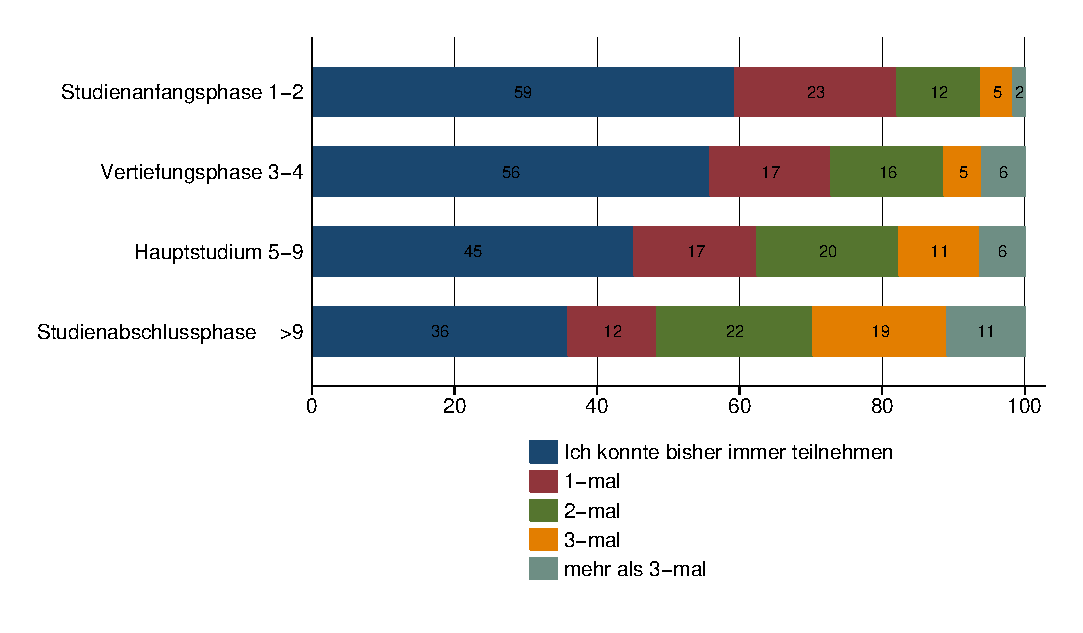
\includegraphics[RemoveGraphicsExtensions={.pdf,PDF}]{image}|
% \end{quote}
%
% \subsection{\plainTeX}
%
% \LaTeX's graphics packages can also be used with \plainTeX.
% The necessary basic \LaTeX\ macros are defined in
% \xfile{miniltx.tex}. This package \xpackage{grfext} also
% relies on it. Example:
%\begin{quote}
%\begin{verbatim}
%\input miniltx.tex\relax
%\def\Gin@driver{pdftex.def}
%\input graphicx.sty\relax
%\input grfext.sty\relax
%\resetatcatcode
%\end{verbatim}
%\end{quote}
%
% \StopEventually{
% }
%
% \section{Implementation}
%
%    \begin{macrocode}
%<*package>
%    \end{macrocode}
%
% \subsection{Relead check and identification}
%    Reload check, especially if the package is not used with \LaTeX.
%    \begin{macrocode}
\begingroup\catcode61\catcode48\catcode32=10\relax%
  \catcode13=5 % ^^M
  \endlinechar=13 %
  \catcode35=6 % #
  \catcode39=12 % '
  \catcode44=12 % ,
  \catcode45=12 % -
  \catcode46=12 % .
  \catcode58=12 % :
  \catcode64=11 % @
  \catcode123=1 % {
  \catcode125=2 % }
  \expandafter\let\expandafter\x\csname ver@grfext.sty\endcsname
  \ifx\x\relax % plain-TeX, first loading
  \else
    \def\empty{}%
    \ifx\x\empty % LaTeX, first loading,
      % variable is initialized, but \ProvidesPackage not yet seen
    \else
      \expandafter\ifx\csname PackageInfo\endcsname\relax
        \def\x#1#2{%
          \immediate\write-1{Package #1 Info: #2.}%
        }%
      \else
        \def\x#1#2{\PackageInfo{#1}{#2, stopped}}%
      \fi
      \x{grfext}{The package is already loaded}%
      \aftergroup\endinput
    \fi
  \fi
\endgroup%
%    \end{macrocode}
%    Package identification:
%    \begin{macrocode}
\begingroup\catcode61\catcode48\catcode32=10\relax%
  \catcode13=5 % ^^M
  \endlinechar=13 %
  \catcode35=6 % #
  \catcode39=12 % '
  \catcode40=12 % (
  \catcode41=12 % )
  \catcode44=12 % ,
  \catcode45=12 % -
  \catcode46=12 % .
  \catcode47=12 % /
  \catcode58=12 % :
  \catcode64=11 % @
  \catcode91=12 % [
  \catcode93=12 % ]
  \catcode123=1 % {
  \catcode125=2 % }
  \expandafter\ifx\csname ProvidesPackage\endcsname\relax
    \def\x#1#2#3[#4]{\endgroup
      \immediate\write-1{Package: #3 #4}%
      \xdef#1{#4}%
    }%
  \else
    \def\x#1#2[#3]{\endgroup
      #2[{#3}]%
      \ifx#1\@undefined
        \xdef#1{#3}%
      \fi
      \ifx#1\relax
        \xdef#1{#3}%
      \fi
    }%
  \fi
\expandafter\x\csname ver@grfext.sty\endcsname
\ProvidesPackage{grfext}%
  [2019/12/03 v1.3 Manage graphics extensions (HO)]%
%    \end{macrocode}
%
% \subsection{Catcodes}
%
%    \begin{macrocode}
\begingroup\catcode61\catcode48\catcode32=10\relax%
  \catcode13=5 % ^^M
  \endlinechar=13 %
  \catcode123=1 % {
  \catcode125=2 % }
  \catcode64=11 % @
  \def\x{\endgroup
    \expandafter\edef\csname grfext@AtEnd\endcsname{%
      \endlinechar=\the\endlinechar\relax
      \catcode13=\the\catcode13\relax
      \catcode32=\the\catcode32\relax
      \catcode35=\the\catcode35\relax
      \catcode61=\the\catcode61\relax
      \catcode64=\the\catcode64\relax
      \catcode123=\the\catcode123\relax
      \catcode125=\the\catcode125\relax
    }%
  }%
\x\catcode61\catcode48\catcode32=10\relax%
\catcode13=5 % ^^M
\endlinechar=13 %
\catcode35=6 % #
\catcode64=11 % @
\catcode123=1 % {
\catcode125=2 % }
\def\TMP@EnsureCode#1#2{%
  \edef\grfext@AtEnd{%
    \grfext@AtEnd
    \catcode#1=\the\catcode#1\relax
  }%
  \catcode#1=#2\relax
}
\TMP@EnsureCode{42}{12}% *
\TMP@EnsureCode{44}{12}% ,
\TMP@EnsureCode{47}{12}% /
\TMP@EnsureCode{58}{12}% :
\TMP@EnsureCode{60}{12}% <
\TMP@EnsureCode{62}{12}% >
\TMP@EnsureCode{91}{12}% [
\TMP@EnsureCode{93}{12}% ]
\edef\grfext@AtEnd{\grfext@AtEnd\noexpand\endinput}
%    \end{macrocode}
%
% \subsection{\plainTeX}
%
%    \begin{macro}{\@expandtwoargs}
%    Requirement is \xfile{miniltx.tex}, but we need also
%    \LaTeX's \cs{@expandtwoargs}.
%    \begin{macrocode}
\@ifundefined{@expandtwoargs}{%
  \def\@expandtwoargs#1#2#3{%
    \edef\reserved@a{\noexpand#1{#2}{#3}}%
    \reserved@a
  }%
}{}
%    \end{macrocode}
%    \end{macro}
%
% \subsection{Add}
%
%    \begin{macro}{\AppendGraphicsExtensions}
%    \begin{macrocode}
\newcommand*{\AppendGraphicsExtensions}{%
  \@ifundefined{Gin@extensions}{%
    \let\Gin@extensions\@empty
  }{}%
  \@ifstar{\grfext@Append\grfext@Check}{\grfext@Append\grfext@@Add}%
}%
%    \end{macrocode}
%    \end{macro}
%    \begin{macro}{\grfext@Append}
%    \begin{macrocode}
\def\grfext@Append#1#2{%
  \let\grfext@Print\@gobble
  \edef\grfext@next{%
    \noexpand\grfext@Add\noexpand#1{%
      \zap@space#2 \@empty
    }{\noexpand\Gin@extensions,}{}%
  }%
  \grfext@next
  \let\grfext@Print\grfext@@Print
  \grfext@Print\AppendGraphicsExtensions
}
%    \end{macrocode}
%    \end{macro}
%
%    \begin{macro}{\PrependGraphicsExtensions}
%    \begin{macrocode}
\newcommand*{\PrependGraphicsExtensions}{%
  \@ifundefined{Gin@extensions}{%
    \let\Gin@extensions\@empty
  }{}%
  \@ifstar{\grfext@Prepend\grfext@Check}{\grfext@Prepend\grfext@@Add}%
}%
%    \end{macrocode}
%    \end{macro}
%    \begin{macro}{\grfext@Prepend}
%    \begin{macrocode}
\def\grfext@Prepend#1#2{%
  \let\grfext@Print\@gobble
  \edef\grfext@next{%
    \noexpand\grfext@Add\noexpand#1{%
      \zap@space#2 \@empty
    }{}{,\noexpand\Gin@extensions}%
  }%
  \grfext@next
  \let\grfext@Print\grfext@@Print
  \grfext@Print\PrependGraphicsExtensions
}
%    \end{macrocode}
%    \end{macro}
%
%    \begin{macro}{\grfext@Add}
%    \begin{macrocode}
\def\grfext@Add#1#2{%
  #1{#2}%
}
%    \end{macrocode}
%    \end{macro}
%    \begin{macro}{\grfext@@Add}
%    \begin{macrocode}
\def\grfext@@Add#1#2#3{%
  \RemoveGraphicsExtensions{#1}%
  \ifx\Gin@extensions\@empty
    \def\Gin@extensions{#1}%
  \else
    \edef\Gin@extensions{#2#1#3}%
  \fi
}
%    \end{macrocode}
%    \end{macro}
%
% \subsection{Check}
%
%    \begin{macro}{\grfext@Check}
%    \begin{macrocode}
\def\grfext@Check#1{%
  \let\grfext@tmp\@empty
  \@for\grfext@ext:=#1\do{%
    \@ifundefined{Gin@rule@\grfext@ext}{%
    }{%
      \ifx\grfext@tmp\@empty
        \let\grfext@tmp\grfext@ext
      \else
        \edef\grfext@tmp{\grfext@tmp,\grfext@ext}%
      \fi
    }%
  }%
  \ifx\grfext@tmp\@empty
    \def\grfext@next##1##2{}%
  \else
    \edef\grfext@next{%
      \noexpand\grfext@@Add{\grfext@tmp}%
    }%
  \fi
  \grfext@next
}
%    \end{macrocode}
%    \end{macro}
%
% \subsection{Remove}
%
%    \begin{macro}{\RemoveGraphicsExtensions}
%    \begin{macrocode}
\newcommand*{\RemoveGraphicsExtensions}[1]{%
  \@ifundefined{Gin@extensions}{%
    \def\Gin@extensions{}%
  }{%
    \edef\grfext@tmp{\zap@space#1 \@empty}%
    \@for\grfext@ext:=\grfext@tmp\do{%
      \def\grfext@next{%
        \let\grfext@tmp\Gin@extensions
        \@expandtwoargs
        \@removeelement\grfext@ext\Gin@extensions\Gin@extensions
        \ifx\grfext@tmp\Gin@extensions
          \let\grfext@next\relax
        \fi
        \grfext@next
      }%
      \grfext@next
    }%
  }%
  \grfext@Print\RemoveGraphicsExtensions
}
%    \end{macrocode}
%    \end{macro}
%
% \subsection{Print}
%
%    \begin{macrocode}
\RequirePackage{infwarerr}[2007/09/09]
%    \end{macrocode}
%
%    \begin{macro}{\PrintGraphicsExtensions}
%    \begin{macrocode}
\def\PrintGraphicsExtensions{%
  \grfext@Print\PrintGraphicsExtensions
}
%    \end{macrocode}
%    \end{macro}
%    \begin{macro}{\grfext@Print}
%    \begin{macrocode}
\def\grfext@Print#1{%
  \@PackageInfo{grfext}{%
    Graphics extension search list:\MessageBreak
    \@ifundefined{Gin@extensions}{%
      <unavailable>%
    }{%
      [\Gin@extensions]%
    }\MessageBreak
    \string#1%
  }%
}
%    \end{macrocode}
%    \end{macro}
%    \begin{macro}{\grfext@@Print}
%    \begin{macrocode}
\let\grfext@@Print\grfext@Print
%    \end{macrocode}
%    \end{macro}
%
% \subsection{Defining options for package \xpackage{graphicx}}
%
%    \begin{macrocode}
\RequirePackage{kvdefinekeys}[2010/03/01]
\kv@define@key{Gin}{AppendGraphicsExtensions}{%
  \AppendGraphicsExtensions{#1}%
}
\kv@define@key{Gin}{AppendGraphicsExtensions*}{%
  \AppendGraphicsExtensions*{#1}%
}
\kv@define@key{Gin}{PrependGraphicsExtensions}{%
  \PrependGraphicsExtensions{#1}%
}
\kv@define@key{Gin}{PrependGraphicsExtensions*}{%
  \PrependGraphicsExtensions*{#1}%
}
\kv@define@key{Gin}{RemoveGraphicsExtensions}{%
  \RemoveGraphicsExtensions{#1}%
}
\kv@define@key{Gin}{PrintGraphicsExtensions}[]{%
  \PrintGraphicsExtensions
}
%    \end{macrocode}
%
%    \begin{macrocode}
\grfext@AtEnd%
%</package>
%    \end{macrocode}
% \section{Installation}
%
% \subsection{Download}
%
% \paragraph{Package.} This package is available on
% CTAN\footnote{\CTANpkg{grfext}}:
% \begin{description}
% \item[\CTAN{macros/latex/contrib/grfext/grfext.dtx}] The source file.
% \item[\CTAN{macros/latex/contrib/grfext/grfext.pdf}] Documentation.
% \end{description}
%
%
% \paragraph{Bundle.} All the packages of the bundle `grfext'
% are also available in a TDS compliant ZIP archive. There
% the packages are already unpacked and the documentation files
% are generated. The files and directories obey the TDS standard.
% \begin{description}
% \item[\CTANinstall{install/macros/latex/contrib/grfext.tds.zip}]
% \end{description}
% \emph{TDS} refers to the standard ``A Directory Structure
% for \TeX\ Files'' (\CTANpkg{tds}). Directories
% with \xfile{texmf} in their name are usually organized this way.
%
% \subsection{Bundle installation}
%
% \paragraph{Unpacking.} Unpack the \xfile{grfext.tds.zip} in the
% TDS tree (also known as \xfile{texmf} tree) of your choice.
% Example (linux):
% \begin{quote}
%   |unzip grfext.tds.zip -d ~/texmf|
% \end{quote}
%
% \subsection{Package installation}
%
% \paragraph{Unpacking.} The \xfile{.dtx} file is a self-extracting
% \docstrip\ archive. The files are extracted by running the
% \xfile{.dtx} through \plainTeX:
% \begin{quote}
%   \verb|tex grfext.dtx|
% \end{quote}
%
% \paragraph{TDS.} Now the different files must be moved into
% the different directories in your installation TDS tree
% (also known as \xfile{texmf} tree):
% \begin{quote}
% \def\t{^^A
% \begin{tabular}{@{}>{\ttfamily}l@{ $\rightarrow$ }>{\ttfamily}l@{}}
%   grfext.sty & tex/latex/grfext/grfext.sty\\
%   grfext.pdf & doc/latex/grfext/grfext.pdf\\
%   grfext.dtx & source/latex/grfext/grfext.dtx\\
% \end{tabular}^^A
% }^^A
% \sbox0{\t}^^A
% \ifdim\wd0>\linewidth
%   \begingroup
%     \advance\linewidth by\leftmargin
%     \advance\linewidth by\rightmargin
%   \edef\x{\endgroup
%     \def\noexpand\lw{\the\linewidth}^^A
%   }\x
%   \def\lwbox{^^A
%     \leavevmode
%     \hbox to \linewidth{^^A
%       \kern-\leftmargin\relax
%       \hss
%       \usebox0
%       \hss
%       \kern-\rightmargin\relax
%     }^^A
%   }^^A
%   \ifdim\wd0>\lw
%     \sbox0{\small\t}^^A
%     \ifdim\wd0>\linewidth
%       \ifdim\wd0>\lw
%         \sbox0{\footnotesize\t}^^A
%         \ifdim\wd0>\linewidth
%           \ifdim\wd0>\lw
%             \sbox0{\scriptsize\t}^^A
%             \ifdim\wd0>\linewidth
%               \ifdim\wd0>\lw
%                 \sbox0{\tiny\t}^^A
%                 \ifdim\wd0>\linewidth
%                   \lwbox
%                 \else
%                   \usebox0
%                 \fi
%               \else
%                 \lwbox
%               \fi
%             \else
%               \usebox0
%             \fi
%           \else
%             \lwbox
%           \fi
%         \else
%           \usebox0
%         \fi
%       \else
%         \lwbox
%       \fi
%     \else
%       \usebox0
%     \fi
%   \else
%     \lwbox
%   \fi
% \else
%   \usebox0
% \fi
% \end{quote}
% If you have a \xfile{docstrip.cfg} that configures and enables \docstrip's
% TDS installing feature, then some files can already be in the right
% place, see the documentation of \docstrip.
%
% \subsection{Refresh file name databases}
%
% If your \TeX~distribution
% (\TeX\,Live, \mikTeX, \dots) relies on file name databases, you must refresh
% these. For example, \TeX\,Live\ users run \verb|texhash| or
% \verb|mktexlsr|.
%
% \subsection{Some details for the interested}
%
% \paragraph{Unpacking with \LaTeX.}
% The \xfile{.dtx} chooses its action depending on the format:
% \begin{description}
% \item[\plainTeX:] Run \docstrip\ and extract the files.
% \item[\LaTeX:] Generate the documentation.
% \end{description}
% If you insist on using \LaTeX\ for \docstrip\ (really,
% \docstrip\ does not need \LaTeX), then inform the autodetect routine
% about your intention:
% \begin{quote}
%   \verb|latex \let\install=y\input{grfext.dtx}|
% \end{quote}
% Do not forget to quote the argument according to the demands
% of your shell.
%
% \paragraph{Generating the documentation.}
% You can use both the \xfile{.dtx} or the \xfile{.drv} to generate
% the documentation. The process can be configured by the
% configuration file \xfile{ltxdoc.cfg}. For instance, put this
% line into this file, if you want to have A4 as paper format:
% \begin{quote}
%   \verb|\PassOptionsToClass{a4paper}{article}|
% \end{quote}
% An example follows how to generate the
% documentation with pdf\LaTeX:
% \begin{quote}
%\begin{verbatim}
%pdflatex grfext.dtx
%makeindex -s gind.ist grfext.idx
%pdflatex grfext.dtx
%makeindex -s gind.ist grfext.idx
%pdflatex grfext.dtx
%\end{verbatim}
% \end{quote}
%
% \begin{thebibliography}{9}
%
% \bibitem{graphics}
%   David Carlisle, Sebastian Rahtz: \textit{The \xpackage{graphics} package};
%   2006/02/20 v1.0o;
%   \CTAN{macros/latex/required/graphics/graphics.dtx}.
%
% \end{thebibliography}
%
% \begin{History}
%   \begin{Version}{2007/09/30 v1.0}
%   \item
%     First public version.
%   \end{Version}
%   \begin{Version}{2010/08/19 v1.1}
%   \item
%     User macros are also made available as keyval options for
%     package \xpackage{graphicx}.
%   \end{Version}
%   \begin{Version}{2016/05/16 v1.2}
%   \item
%     Documentation updates.
%   \end{Version}
%   \begin{Version}{2019/12/03 v1.3}
%   \item
%     Documentation updates.
%   \end{Version}
% \end{History}
%
% \PrintIndex
%
% \Finale
\endinput

%        (quote the arguments according to the demands of your shell)
%
% Documentation:
%    (a) If grfext.drv is present:
%           latex grfext.drv
%    (b) Without grfext.drv:
%           latex grfext.dtx; ...
%    The class ltxdoc loads the configuration file ltxdoc.cfg
%    if available. Here you can specify further options, e.g.
%    use A4 as paper format:
%       \PassOptionsToClass{a4paper}{article}
%
%    Programm calls to get the documentation (example):
%       pdflatex grfext.dtx
%       makeindex -s gind.ist grfext.idx
%       pdflatex grfext.dtx
%       makeindex -s gind.ist grfext.idx
%       pdflatex grfext.dtx
%
% Installation:
%    TDS:tex/latex/grfext/grfext.sty
%    TDS:doc/latex/grfext/grfext.pdf
%    TDS:source/latex/grfext/grfext.dtx
%
%<*ignore>
\begingroup
  \catcode123=1 %
  \catcode125=2 %
  \def\x{LaTeX2e}%
\expandafter\endgroup
\ifcase 0\ifx\install y1\fi\expandafter
         \ifx\csname processbatchFile\endcsname\relax\else1\fi
         \ifx\fmtname\x\else 1\fi\relax
\else\csname fi\endcsname
%</ignore>
%<*install>
\input docstrip.tex
\Msg{************************************************************************}
\Msg{* Installation}
\Msg{* Package: grfext 2019/12/03 v1.3 Manage graphics extensions (HO)}
\Msg{************************************************************************}

\keepsilent
\askforoverwritefalse

\let\MetaPrefix\relax
\preamble

This is a generated file.

Project: grfext
Version: 2019/12/03 v1.3

Copyright (C)
   2007, 2010 Heiko Oberdiek
   2016-2019 Oberdiek Package Support Group

This work may be distributed and/or modified under the
conditions of the LaTeX Project Public License, either
version 1.3c of this license or (at your option) any later
version. This version of this license is in
   https://www.latex-project.org/lppl/lppl-1-3c.txt
and the latest version of this license is in
   https://www.latex-project.org/lppl.txt
and version 1.3 or later is part of all distributions of
LaTeX version 2005/12/01 or later.

This work has the LPPL maintenance status "maintained".

The Current Maintainers of this work are
Heiko Oberdiek and the Oberdiek Package Support Group
https://github.com/ho-tex/grfext/issues


This work consists of the main source file grfext.dtx
and the derived files
   grfext.sty, grfext.pdf, grfext.ins, grfext.drv.

\endpreamble
\let\MetaPrefix\DoubleperCent

\generate{%
  \file{grfext.ins}{\from{grfext.dtx}{install}}%
  \file{grfext.drv}{\from{grfext.dtx}{driver}}%
  \usedir{tex/latex/grfext}%
  \file{grfext.sty}{\from{grfext.dtx}{package}}%
%  \usedir{doc/latex/grfext/test}%
%  \file{grfext-test1.tex}{\from{grfext.dtx}{test1}}%
%  \file{grfext-test2.tex}{\from{grfext.dtx}{test2}}%
}

\catcode32=13\relax% active space
\let =\space%
\Msg{************************************************************************}
\Msg{*}
\Msg{* To finish the installation you have to move the following}
\Msg{* file into a directory searched by TeX:}
\Msg{*}
\Msg{*     grfext.sty}
\Msg{*}
\Msg{* To produce the documentation run the file `grfext.drv'}
\Msg{* through LaTeX.}
\Msg{*}
\Msg{* Happy TeXing!}
\Msg{*}
\Msg{************************************************************************}

\endbatchfile
%</install>
%<*ignore>
\fi
%</ignore>
%<*driver>
\NeedsTeXFormat{LaTeX2e}
\ProvidesFile{grfext.drv}%
  [2019/12/03 v1.3 Manage graphics extensions (HO)]%
\documentclass{ltxdoc}
\usepackage{holtxdoc}[2011/11/22]
\begin{document}
  \DocInput{grfext.dtx}%
\end{document}
%</driver>
% \fi
%
%
%
% \GetFileInfo{grfext.drv}
%
% \title{The \xpackage{grfext} package}
% \date{2019/12/03 v1.3}
% \author{Heiko Oberdiek\thanks
% {Please report any issues at \url{https://github.com/ho-tex/grfext/issues}}}
%
% \maketitle
%
% \begin{abstract}
% This package provides macros for adding and reordering
% graphics extensions of package \xpackage{graphics}.
% \end{abstract}
%
% \tableofcontents
%
% \section{Documentation}
%
% \subsection{Introduction}
%
% If you are not familiar with \LaTeX's graphics bundle, please
% read its documentation \xfile{grffile} \cite{graphics}.
% The bundle contains two packages for graphics inclusion:
% \xpackage{graphics} and \xpackage{graphicx}. The first one
% is loaded by the second one that adds a key value interface.
%
% Graphics files are included in both cases by macro
% \cs{includegraphics}. The file name extension can be omitted.
% Then the graphics package goes through a list of known
% extensions until it finds the graphics file. This extension list
% is set by \cs{DeclareGraphicsExtensions}. The previous contents
% of the list is overwritten.
%
% \subsection{User interface}
%
% This package \xpackage{grfext} provides macros that adds entries
% to the list or remove them. The list may be empty or even
% undefined before. It is always defined afterwards, but can
% be empty (especially after removing entries).
%
% \begin{declcs}{AppendGraphicsExtensions} * \M{ext-list}\\
%   \cs{PrependGraphicsExtensions} * \M{ext-list}
% \end{declcs}
% The argument \meta{ext-list} is a comma separated list whose
% entries are file name extensions including the dot.
% But first the entries are removed from
% \xpackage{graphics}' extension list to avoid multiple
% occurences of the same extension.
%
% Then macro \cs{AppendGraphicsExtensions} adds the entries
% after the end of \xpackage{graphics}' list, whereas
% macro \cs{PrependGraphicsExtensions} puts them in front
% of the list.
% The order matters if a graphics file is available in
% different acceptable formats. Then the first extension
% wins.
%
% The star version of these commands only adds an extensions,
% if a specific graphics rule exists for that extension.
%
% \begin{declcs}{RemoveGraphicsExtensions} \M{ext-list}
% \end{declcs}
% All occurences of file extensions in \meta{ext-list} are
% removed from \xpackage{graphics}' extension list.
%
% \subsection{Package loading}
%
% The package does not define any options. It is loaded
% as usual in \LaTeX, e.g.:
% \begin{quote}
%   |\usepackage{grfext}|
% \end{quote}
%
% \begin{declcs}{PrintGraphicsExtensions}
% \end{declcs}
% Macro \cs{PrintGraphicsExtensions} writes the current
% graphics extensions list in the \xfile{.log} file.
% The macros described before do this automatically
% after their operation.
%
% \subsection{Option support for package \xpackage{graphicx}}
%
% Package \xpackage{graphicx} uses the interface of package
% \xpackage{keyval} in order to specify options for
% \cs{includegraphics}. The options can also be set using
% \begin{quote}
%   |\setkeys{Gin}{|\meta{options}|}|
% \end{quote}
% The four user macros with the two star forms are available
% as options in family |Gin| as well:
% \begin{quote}
%   |AppendGraphicsExtensions={|\meta{ext-list}|}|\\
%   |AppendGraphicsExtensions*={|\meta{ext-list}|}|\\
%   |PrependGraphicsExtensions={|\meta{ext-list}|}|\\
%   |PrependGraphicsExtensions*{|\meta{ext-list}|}|\\
%   |RemoveGraphicsExtensions={|\meta{ext-list}|}|\\
%   |PrintGraphicsExtensions|
% \end{quote}
% This makes it easier to locally change the extension list
% for an included graphics, e.g.:
% \begin{quote}
%   |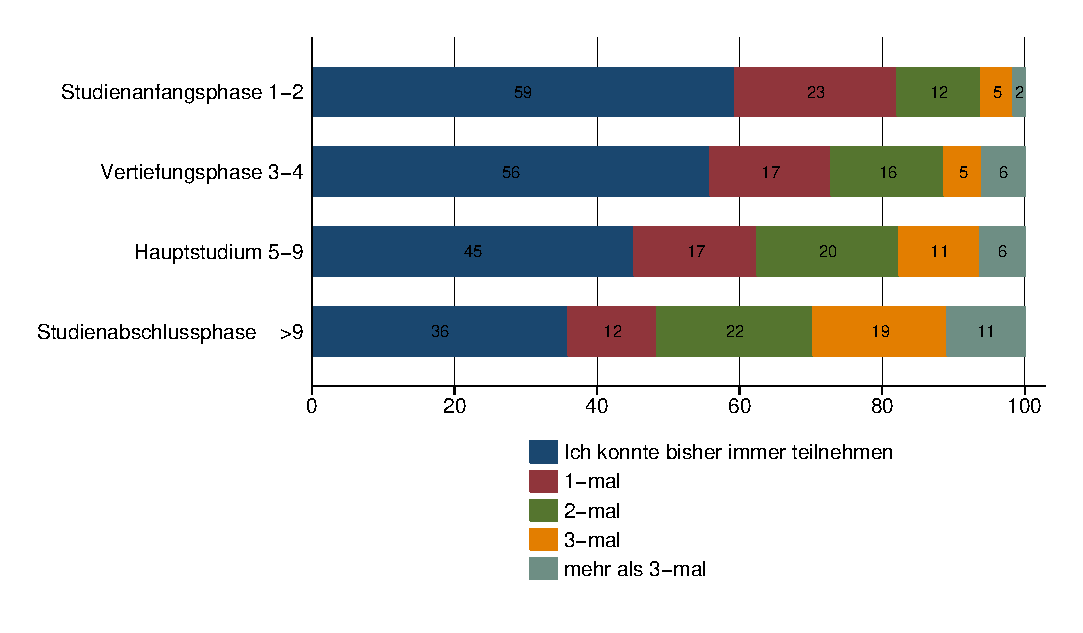
\includegraphics[RemoveGraphicsExtensions={.pdf,PDF}]{image}|
% \end{quote}
%
% \subsection{\plainTeX}
%
% \LaTeX's graphics packages can also be used with \plainTeX.
% The necessary basic \LaTeX\ macros are defined in
% \xfile{miniltx.tex}. This package \xpackage{grfext} also
% relies on it. Example:
%\begin{quote}
%\begin{verbatim}
%\input miniltx.tex\relax
%\def\Gin@driver{pdftex.def}
%\input graphicx.sty\relax
%\input grfext.sty\relax
%\resetatcatcode
%\end{verbatim}
%\end{quote}
%
% \StopEventually{
% }
%
% \section{Implementation}
%
%    \begin{macrocode}
%<*package>
%    \end{macrocode}
%
% \subsection{Relead check and identification}
%    Reload check, especially if the package is not used with \LaTeX.
%    \begin{macrocode}
\begingroup\catcode61\catcode48\catcode32=10\relax%
  \catcode13=5 % ^^M
  \endlinechar=13 %
  \catcode35=6 % #
  \catcode39=12 % '
  \catcode44=12 % ,
  \catcode45=12 % -
  \catcode46=12 % .
  \catcode58=12 % :
  \catcode64=11 % @
  \catcode123=1 % {
  \catcode125=2 % }
  \expandafter\let\expandafter\x\csname ver@grfext.sty\endcsname
  \ifx\x\relax % plain-TeX, first loading
  \else
    \def\empty{}%
    \ifx\x\empty % LaTeX, first loading,
      % variable is initialized, but \ProvidesPackage not yet seen
    \else
      \expandafter\ifx\csname PackageInfo\endcsname\relax
        \def\x#1#2{%
          \immediate\write-1{Package #1 Info: #2.}%
        }%
      \else
        \def\x#1#2{\PackageInfo{#1}{#2, stopped}}%
      \fi
      \x{grfext}{The package is already loaded}%
      \aftergroup\endinput
    \fi
  \fi
\endgroup%
%    \end{macrocode}
%    Package identification:
%    \begin{macrocode}
\begingroup\catcode61\catcode48\catcode32=10\relax%
  \catcode13=5 % ^^M
  \endlinechar=13 %
  \catcode35=6 % #
  \catcode39=12 % '
  \catcode40=12 % (
  \catcode41=12 % )
  \catcode44=12 % ,
  \catcode45=12 % -
  \catcode46=12 % .
  \catcode47=12 % /
  \catcode58=12 % :
  \catcode64=11 % @
  \catcode91=12 % [
  \catcode93=12 % ]
  \catcode123=1 % {
  \catcode125=2 % }
  \expandafter\ifx\csname ProvidesPackage\endcsname\relax
    \def\x#1#2#3[#4]{\endgroup
      \immediate\write-1{Package: #3 #4}%
      \xdef#1{#4}%
    }%
  \else
    \def\x#1#2[#3]{\endgroup
      #2[{#3}]%
      \ifx#1\@undefined
        \xdef#1{#3}%
      \fi
      \ifx#1\relax
        \xdef#1{#3}%
      \fi
    }%
  \fi
\expandafter\x\csname ver@grfext.sty\endcsname
\ProvidesPackage{grfext}%
  [2019/12/03 v1.3 Manage graphics extensions (HO)]%
%    \end{macrocode}
%
% \subsection{Catcodes}
%
%    \begin{macrocode}
\begingroup\catcode61\catcode48\catcode32=10\relax%
  \catcode13=5 % ^^M
  \endlinechar=13 %
  \catcode123=1 % {
  \catcode125=2 % }
  \catcode64=11 % @
  \def\x{\endgroup
    \expandafter\edef\csname grfext@AtEnd\endcsname{%
      \endlinechar=\the\endlinechar\relax
      \catcode13=\the\catcode13\relax
      \catcode32=\the\catcode32\relax
      \catcode35=\the\catcode35\relax
      \catcode61=\the\catcode61\relax
      \catcode64=\the\catcode64\relax
      \catcode123=\the\catcode123\relax
      \catcode125=\the\catcode125\relax
    }%
  }%
\x\catcode61\catcode48\catcode32=10\relax%
\catcode13=5 % ^^M
\endlinechar=13 %
\catcode35=6 % #
\catcode64=11 % @
\catcode123=1 % {
\catcode125=2 % }
\def\TMP@EnsureCode#1#2{%
  \edef\grfext@AtEnd{%
    \grfext@AtEnd
    \catcode#1=\the\catcode#1\relax
  }%
  \catcode#1=#2\relax
}
\TMP@EnsureCode{42}{12}% *
\TMP@EnsureCode{44}{12}% ,
\TMP@EnsureCode{47}{12}% /
\TMP@EnsureCode{58}{12}% :
\TMP@EnsureCode{60}{12}% <
\TMP@EnsureCode{62}{12}% >
\TMP@EnsureCode{91}{12}% [
\TMP@EnsureCode{93}{12}% ]
\edef\grfext@AtEnd{\grfext@AtEnd\noexpand\endinput}
%    \end{macrocode}
%
% \subsection{\plainTeX}
%
%    \begin{macro}{\@expandtwoargs}
%    Requirement is \xfile{miniltx.tex}, but we need also
%    \LaTeX's \cs{@expandtwoargs}.
%    \begin{macrocode}
\@ifundefined{@expandtwoargs}{%
  \def\@expandtwoargs#1#2#3{%
    \edef\reserved@a{\noexpand#1{#2}{#3}}%
    \reserved@a
  }%
}{}
%    \end{macrocode}
%    \end{macro}
%
% \subsection{Add}
%
%    \begin{macro}{\AppendGraphicsExtensions}
%    \begin{macrocode}
\newcommand*{\AppendGraphicsExtensions}{%
  \@ifundefined{Gin@extensions}{%
    \let\Gin@extensions\@empty
  }{}%
  \@ifstar{\grfext@Append\grfext@Check}{\grfext@Append\grfext@@Add}%
}%
%    \end{macrocode}
%    \end{macro}
%    \begin{macro}{\grfext@Append}
%    \begin{macrocode}
\def\grfext@Append#1#2{%
  \let\grfext@Print\@gobble
  \edef\grfext@next{%
    \noexpand\grfext@Add\noexpand#1{%
      \zap@space#2 \@empty
    }{\noexpand\Gin@extensions,}{}%
  }%
  \grfext@next
  \let\grfext@Print\grfext@@Print
  \grfext@Print\AppendGraphicsExtensions
}
%    \end{macrocode}
%    \end{macro}
%
%    \begin{macro}{\PrependGraphicsExtensions}
%    \begin{macrocode}
\newcommand*{\PrependGraphicsExtensions}{%
  \@ifundefined{Gin@extensions}{%
    \let\Gin@extensions\@empty
  }{}%
  \@ifstar{\grfext@Prepend\grfext@Check}{\grfext@Prepend\grfext@@Add}%
}%
%    \end{macrocode}
%    \end{macro}
%    \begin{macro}{\grfext@Prepend}
%    \begin{macrocode}
\def\grfext@Prepend#1#2{%
  \let\grfext@Print\@gobble
  \edef\grfext@next{%
    \noexpand\grfext@Add\noexpand#1{%
      \zap@space#2 \@empty
    }{}{,\noexpand\Gin@extensions}%
  }%
  \grfext@next
  \let\grfext@Print\grfext@@Print
  \grfext@Print\PrependGraphicsExtensions
}
%    \end{macrocode}
%    \end{macro}
%
%    \begin{macro}{\grfext@Add}
%    \begin{macrocode}
\def\grfext@Add#1#2{%
  #1{#2}%
}
%    \end{macrocode}
%    \end{macro}
%    \begin{macro}{\grfext@@Add}
%    \begin{macrocode}
\def\grfext@@Add#1#2#3{%
  \RemoveGraphicsExtensions{#1}%
  \ifx\Gin@extensions\@empty
    \def\Gin@extensions{#1}%
  \else
    \edef\Gin@extensions{#2#1#3}%
  \fi
}
%    \end{macrocode}
%    \end{macro}
%
% \subsection{Check}
%
%    \begin{macro}{\grfext@Check}
%    \begin{macrocode}
\def\grfext@Check#1{%
  \let\grfext@tmp\@empty
  \@for\grfext@ext:=#1\do{%
    \@ifundefined{Gin@rule@\grfext@ext}{%
    }{%
      \ifx\grfext@tmp\@empty
        \let\grfext@tmp\grfext@ext
      \else
        \edef\grfext@tmp{\grfext@tmp,\grfext@ext}%
      \fi
    }%
  }%
  \ifx\grfext@tmp\@empty
    \def\grfext@next##1##2{}%
  \else
    \edef\grfext@next{%
      \noexpand\grfext@@Add{\grfext@tmp}%
    }%
  \fi
  \grfext@next
}
%    \end{macrocode}
%    \end{macro}
%
% \subsection{Remove}
%
%    \begin{macro}{\RemoveGraphicsExtensions}
%    \begin{macrocode}
\newcommand*{\RemoveGraphicsExtensions}[1]{%
  \@ifundefined{Gin@extensions}{%
    \def\Gin@extensions{}%
  }{%
    \edef\grfext@tmp{\zap@space#1 \@empty}%
    \@for\grfext@ext:=\grfext@tmp\do{%
      \def\grfext@next{%
        \let\grfext@tmp\Gin@extensions
        \@expandtwoargs
        \@removeelement\grfext@ext\Gin@extensions\Gin@extensions
        \ifx\grfext@tmp\Gin@extensions
          \let\grfext@next\relax
        \fi
        \grfext@next
      }%
      \grfext@next
    }%
  }%
  \grfext@Print\RemoveGraphicsExtensions
}
%    \end{macrocode}
%    \end{macro}
%
% \subsection{Print}
%
%    \begin{macrocode}
\RequirePackage{infwarerr}[2007/09/09]
%    \end{macrocode}
%
%    \begin{macro}{\PrintGraphicsExtensions}
%    \begin{macrocode}
\def\PrintGraphicsExtensions{%
  \grfext@Print\PrintGraphicsExtensions
}
%    \end{macrocode}
%    \end{macro}
%    \begin{macro}{\grfext@Print}
%    \begin{macrocode}
\def\grfext@Print#1{%
  \@PackageInfo{grfext}{%
    Graphics extension search list:\MessageBreak
    \@ifundefined{Gin@extensions}{%
      <unavailable>%
    }{%
      [\Gin@extensions]%
    }\MessageBreak
    \string#1%
  }%
}
%    \end{macrocode}
%    \end{macro}
%    \begin{macro}{\grfext@@Print}
%    \begin{macrocode}
\let\grfext@@Print\grfext@Print
%    \end{macrocode}
%    \end{macro}
%
% \subsection{Defining options for package \xpackage{graphicx}}
%
%    \begin{macrocode}
\RequirePackage{kvdefinekeys}[2010/03/01]
\kv@define@key{Gin}{AppendGraphicsExtensions}{%
  \AppendGraphicsExtensions{#1}%
}
\kv@define@key{Gin}{AppendGraphicsExtensions*}{%
  \AppendGraphicsExtensions*{#1}%
}
\kv@define@key{Gin}{PrependGraphicsExtensions}{%
  \PrependGraphicsExtensions{#1}%
}
\kv@define@key{Gin}{PrependGraphicsExtensions*}{%
  \PrependGraphicsExtensions*{#1}%
}
\kv@define@key{Gin}{RemoveGraphicsExtensions}{%
  \RemoveGraphicsExtensions{#1}%
}
\kv@define@key{Gin}{PrintGraphicsExtensions}[]{%
  \PrintGraphicsExtensions
}
%    \end{macrocode}
%
%    \begin{macrocode}
\grfext@AtEnd%
%</package>
%    \end{macrocode}
% \section{Installation}
%
% \subsection{Download}
%
% \paragraph{Package.} This package is available on
% CTAN\footnote{\CTANpkg{grfext}}:
% \begin{description}
% \item[\CTAN{macros/latex/contrib/grfext/grfext.dtx}] The source file.
% \item[\CTAN{macros/latex/contrib/grfext/grfext.pdf}] Documentation.
% \end{description}
%
%
% \paragraph{Bundle.} All the packages of the bundle `grfext'
% are also available in a TDS compliant ZIP archive. There
% the packages are already unpacked and the documentation files
% are generated. The files and directories obey the TDS standard.
% \begin{description}
% \item[\CTANinstall{install/macros/latex/contrib/grfext.tds.zip}]
% \end{description}
% \emph{TDS} refers to the standard ``A Directory Structure
% for \TeX\ Files'' (\CTANpkg{tds}). Directories
% with \xfile{texmf} in their name are usually organized this way.
%
% \subsection{Bundle installation}
%
% \paragraph{Unpacking.} Unpack the \xfile{grfext.tds.zip} in the
% TDS tree (also known as \xfile{texmf} tree) of your choice.
% Example (linux):
% \begin{quote}
%   |unzip grfext.tds.zip -d ~/texmf|
% \end{quote}
%
% \subsection{Package installation}
%
% \paragraph{Unpacking.} The \xfile{.dtx} file is a self-extracting
% \docstrip\ archive. The files are extracted by running the
% \xfile{.dtx} through \plainTeX:
% \begin{quote}
%   \verb|tex grfext.dtx|
% \end{quote}
%
% \paragraph{TDS.} Now the different files must be moved into
% the different directories in your installation TDS tree
% (also known as \xfile{texmf} tree):
% \begin{quote}
% \def\t{^^A
% \begin{tabular}{@{}>{\ttfamily}l@{ $\rightarrow$ }>{\ttfamily}l@{}}
%   grfext.sty & tex/latex/grfext/grfext.sty\\
%   grfext.pdf & doc/latex/grfext/grfext.pdf\\
%   grfext.dtx & source/latex/grfext/grfext.dtx\\
% \end{tabular}^^A
% }^^A
% \sbox0{\t}^^A
% \ifdim\wd0>\linewidth
%   \begingroup
%     \advance\linewidth by\leftmargin
%     \advance\linewidth by\rightmargin
%   \edef\x{\endgroup
%     \def\noexpand\lw{\the\linewidth}^^A
%   }\x
%   \def\lwbox{^^A
%     \leavevmode
%     \hbox to \linewidth{^^A
%       \kern-\leftmargin\relax
%       \hss
%       \usebox0
%       \hss
%       \kern-\rightmargin\relax
%     }^^A
%   }^^A
%   \ifdim\wd0>\lw
%     \sbox0{\small\t}^^A
%     \ifdim\wd0>\linewidth
%       \ifdim\wd0>\lw
%         \sbox0{\footnotesize\t}^^A
%         \ifdim\wd0>\linewidth
%           \ifdim\wd0>\lw
%             \sbox0{\scriptsize\t}^^A
%             \ifdim\wd0>\linewidth
%               \ifdim\wd0>\lw
%                 \sbox0{\tiny\t}^^A
%                 \ifdim\wd0>\linewidth
%                   \lwbox
%                 \else
%                   \usebox0
%                 \fi
%               \else
%                 \lwbox
%               \fi
%             \else
%               \usebox0
%             \fi
%           \else
%             \lwbox
%           \fi
%         \else
%           \usebox0
%         \fi
%       \else
%         \lwbox
%       \fi
%     \else
%       \usebox0
%     \fi
%   \else
%     \lwbox
%   \fi
% \else
%   \usebox0
% \fi
% \end{quote}
% If you have a \xfile{docstrip.cfg} that configures and enables \docstrip's
% TDS installing feature, then some files can already be in the right
% place, see the documentation of \docstrip.
%
% \subsection{Refresh file name databases}
%
% If your \TeX~distribution
% (\TeX\,Live, \mikTeX, \dots) relies on file name databases, you must refresh
% these. For example, \TeX\,Live\ users run \verb|texhash| or
% \verb|mktexlsr|.
%
% \subsection{Some details for the interested}
%
% \paragraph{Unpacking with \LaTeX.}
% The \xfile{.dtx} chooses its action depending on the format:
% \begin{description}
% \item[\plainTeX:] Run \docstrip\ and extract the files.
% \item[\LaTeX:] Generate the documentation.
% \end{description}
% If you insist on using \LaTeX\ for \docstrip\ (really,
% \docstrip\ does not need \LaTeX), then inform the autodetect routine
% about your intention:
% \begin{quote}
%   \verb|latex \let\install=y% \iffalse meta-comment
%
% File: grfext.dtx
% Version: 2019/12/03 v1.3
% Info: Manage graphics extensions
%
% Copyright (C)
%    2007, 2010 Heiko Oberdiek
%    2016-2019 Oberdiek Package Support Group
%    https://github.com/ho-tex/grfext/issues
%
% This work may be distributed and/or modified under the
% conditions of the LaTeX Project Public License, either
% version 1.3c of this license or (at your option) any later
% version. This version of this license is in
%    https://www.latex-project.org/lppl/lppl-1-3c.txt
% and the latest version of this license is in
%    https://www.latex-project.org/lppl.txt
% and version 1.3 or later is part of all distributions of
% LaTeX version 2005/12/01 or later.
%
% This work has the LPPL maintenance status "maintained".
%
% The Current Maintainers of this work are
% Heiko Oberdiek and the Oberdiek Package Support Group
% https://github.com/ho-tex/grfext/issues
%
% This work consists of the main source file grfext.dtx
% and the derived files
%    grfext.sty, grfext.pdf, grfext.ins, grfext.drv,
%
% Distribution:
%    CTAN:macros/latex/contrib/grfext/grfext.dtx
%    CTAN:macros/latex/contrib/grfext/grfext.pdf
%
% Unpacking:
%    (a) If grfext.ins is present:
%           tex grfext.ins
%    (b) Without grfext.ins:
%           tex grfext.dtx
%    (c) If you insist on using LaTeX
%           latex \let\install=y\input{grfext.dtx}
%        (quote the arguments according to the demands of your shell)
%
% Documentation:
%    (a) If grfext.drv is present:
%           latex grfext.drv
%    (b) Without grfext.drv:
%           latex grfext.dtx; ...
%    The class ltxdoc loads the configuration file ltxdoc.cfg
%    if available. Here you can specify further options, e.g.
%    use A4 as paper format:
%       \PassOptionsToClass{a4paper}{article}
%
%    Programm calls to get the documentation (example):
%       pdflatex grfext.dtx
%       makeindex -s gind.ist grfext.idx
%       pdflatex grfext.dtx
%       makeindex -s gind.ist grfext.idx
%       pdflatex grfext.dtx
%
% Installation:
%    TDS:tex/latex/grfext/grfext.sty
%    TDS:doc/latex/grfext/grfext.pdf
%    TDS:source/latex/grfext/grfext.dtx
%
%<*ignore>
\begingroup
  \catcode123=1 %
  \catcode125=2 %
  \def\x{LaTeX2e}%
\expandafter\endgroup
\ifcase 0\ifx\install y1\fi\expandafter
         \ifx\csname processbatchFile\endcsname\relax\else1\fi
         \ifx\fmtname\x\else 1\fi\relax
\else\csname fi\endcsname
%</ignore>
%<*install>
\input docstrip.tex
\Msg{************************************************************************}
\Msg{* Installation}
\Msg{* Package: grfext 2019/12/03 v1.3 Manage graphics extensions (HO)}
\Msg{************************************************************************}

\keepsilent
\askforoverwritefalse

\let\MetaPrefix\relax
\preamble

This is a generated file.

Project: grfext
Version: 2019/12/03 v1.3

Copyright (C)
   2007, 2010 Heiko Oberdiek
   2016-2019 Oberdiek Package Support Group

This work may be distributed and/or modified under the
conditions of the LaTeX Project Public License, either
version 1.3c of this license or (at your option) any later
version. This version of this license is in
   https://www.latex-project.org/lppl/lppl-1-3c.txt
and the latest version of this license is in
   https://www.latex-project.org/lppl.txt
and version 1.3 or later is part of all distributions of
LaTeX version 2005/12/01 or later.

This work has the LPPL maintenance status "maintained".

The Current Maintainers of this work are
Heiko Oberdiek and the Oberdiek Package Support Group
https://github.com/ho-tex/grfext/issues


This work consists of the main source file grfext.dtx
and the derived files
   grfext.sty, grfext.pdf, grfext.ins, grfext.drv.

\endpreamble
\let\MetaPrefix\DoubleperCent

\generate{%
  \file{grfext.ins}{\from{grfext.dtx}{install}}%
  \file{grfext.drv}{\from{grfext.dtx}{driver}}%
  \usedir{tex/latex/grfext}%
  \file{grfext.sty}{\from{grfext.dtx}{package}}%
%  \usedir{doc/latex/grfext/test}%
%  \file{grfext-test1.tex}{\from{grfext.dtx}{test1}}%
%  \file{grfext-test2.tex}{\from{grfext.dtx}{test2}}%
}

\catcode32=13\relax% active space
\let =\space%
\Msg{************************************************************************}
\Msg{*}
\Msg{* To finish the installation you have to move the following}
\Msg{* file into a directory searched by TeX:}
\Msg{*}
\Msg{*     grfext.sty}
\Msg{*}
\Msg{* To produce the documentation run the file `grfext.drv'}
\Msg{* through LaTeX.}
\Msg{*}
\Msg{* Happy TeXing!}
\Msg{*}
\Msg{************************************************************************}

\endbatchfile
%</install>
%<*ignore>
\fi
%</ignore>
%<*driver>
\NeedsTeXFormat{LaTeX2e}
\ProvidesFile{grfext.drv}%
  [2019/12/03 v1.3 Manage graphics extensions (HO)]%
\documentclass{ltxdoc}
\usepackage{holtxdoc}[2011/11/22]
\begin{document}
  \DocInput{grfext.dtx}%
\end{document}
%</driver>
% \fi
%
%
%
% \GetFileInfo{grfext.drv}
%
% \title{The \xpackage{grfext} package}
% \date{2019/12/03 v1.3}
% \author{Heiko Oberdiek\thanks
% {Please report any issues at \url{https://github.com/ho-tex/grfext/issues}}}
%
% \maketitle
%
% \begin{abstract}
% This package provides macros for adding and reordering
% graphics extensions of package \xpackage{graphics}.
% \end{abstract}
%
% \tableofcontents
%
% \section{Documentation}
%
% \subsection{Introduction}
%
% If you are not familiar with \LaTeX's graphics bundle, please
% read its documentation \xfile{grffile} \cite{graphics}.
% The bundle contains two packages for graphics inclusion:
% \xpackage{graphics} and \xpackage{graphicx}. The first one
% is loaded by the second one that adds a key value interface.
%
% Graphics files are included in both cases by macro
% \cs{includegraphics}. The file name extension can be omitted.
% Then the graphics package goes through a list of known
% extensions until it finds the graphics file. This extension list
% is set by \cs{DeclareGraphicsExtensions}. The previous contents
% of the list is overwritten.
%
% \subsection{User interface}
%
% This package \xpackage{grfext} provides macros that adds entries
% to the list or remove them. The list may be empty or even
% undefined before. It is always defined afterwards, but can
% be empty (especially after removing entries).
%
% \begin{declcs}{AppendGraphicsExtensions} * \M{ext-list}\\
%   \cs{PrependGraphicsExtensions} * \M{ext-list}
% \end{declcs}
% The argument \meta{ext-list} is a comma separated list whose
% entries are file name extensions including the dot.
% But first the entries are removed from
% \xpackage{graphics}' extension list to avoid multiple
% occurences of the same extension.
%
% Then macro \cs{AppendGraphicsExtensions} adds the entries
% after the end of \xpackage{graphics}' list, whereas
% macro \cs{PrependGraphicsExtensions} puts them in front
% of the list.
% The order matters if a graphics file is available in
% different acceptable formats. Then the first extension
% wins.
%
% The star version of these commands only adds an extensions,
% if a specific graphics rule exists for that extension.
%
% \begin{declcs}{RemoveGraphicsExtensions} \M{ext-list}
% \end{declcs}
% All occurences of file extensions in \meta{ext-list} are
% removed from \xpackage{graphics}' extension list.
%
% \subsection{Package loading}
%
% The package does not define any options. It is loaded
% as usual in \LaTeX, e.g.:
% \begin{quote}
%   |\usepackage{grfext}|
% \end{quote}
%
% \begin{declcs}{PrintGraphicsExtensions}
% \end{declcs}
% Macro \cs{PrintGraphicsExtensions} writes the current
% graphics extensions list in the \xfile{.log} file.
% The macros described before do this automatically
% after their operation.
%
% \subsection{Option support for package \xpackage{graphicx}}
%
% Package \xpackage{graphicx} uses the interface of package
% \xpackage{keyval} in order to specify options for
% \cs{includegraphics}. The options can also be set using
% \begin{quote}
%   |\setkeys{Gin}{|\meta{options}|}|
% \end{quote}
% The four user macros with the two star forms are available
% as options in family |Gin| as well:
% \begin{quote}
%   |AppendGraphicsExtensions={|\meta{ext-list}|}|\\
%   |AppendGraphicsExtensions*={|\meta{ext-list}|}|\\
%   |PrependGraphicsExtensions={|\meta{ext-list}|}|\\
%   |PrependGraphicsExtensions*{|\meta{ext-list}|}|\\
%   |RemoveGraphicsExtensions={|\meta{ext-list}|}|\\
%   |PrintGraphicsExtensions|
% \end{quote}
% This makes it easier to locally change the extension list
% for an included graphics, e.g.:
% \begin{quote}
%   |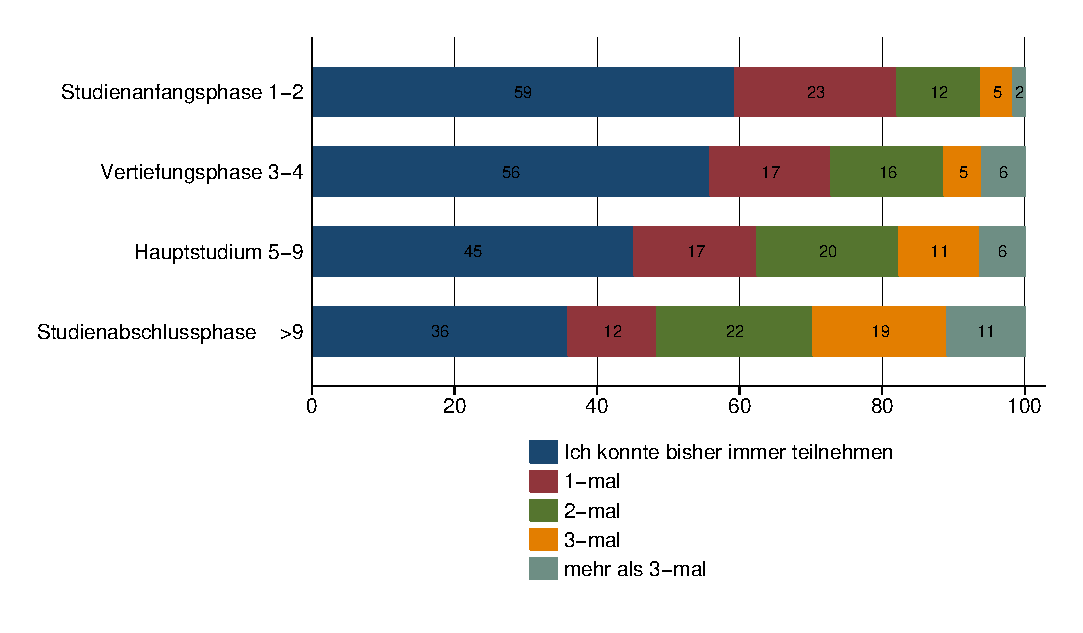
\includegraphics[RemoveGraphicsExtensions={.pdf,PDF}]{image}|
% \end{quote}
%
% \subsection{\plainTeX}
%
% \LaTeX's graphics packages can also be used with \plainTeX.
% The necessary basic \LaTeX\ macros are defined in
% \xfile{miniltx.tex}. This package \xpackage{grfext} also
% relies on it. Example:
%\begin{quote}
%\begin{verbatim}
%\input miniltx.tex\relax
%\def\Gin@driver{pdftex.def}
%\input graphicx.sty\relax
%\input grfext.sty\relax
%\resetatcatcode
%\end{verbatim}
%\end{quote}
%
% \StopEventually{
% }
%
% \section{Implementation}
%
%    \begin{macrocode}
%<*package>
%    \end{macrocode}
%
% \subsection{Relead check and identification}
%    Reload check, especially if the package is not used with \LaTeX.
%    \begin{macrocode}
\begingroup\catcode61\catcode48\catcode32=10\relax%
  \catcode13=5 % ^^M
  \endlinechar=13 %
  \catcode35=6 % #
  \catcode39=12 % '
  \catcode44=12 % ,
  \catcode45=12 % -
  \catcode46=12 % .
  \catcode58=12 % :
  \catcode64=11 % @
  \catcode123=1 % {
  \catcode125=2 % }
  \expandafter\let\expandafter\x\csname ver@grfext.sty\endcsname
  \ifx\x\relax % plain-TeX, first loading
  \else
    \def\empty{}%
    \ifx\x\empty % LaTeX, first loading,
      % variable is initialized, but \ProvidesPackage not yet seen
    \else
      \expandafter\ifx\csname PackageInfo\endcsname\relax
        \def\x#1#2{%
          \immediate\write-1{Package #1 Info: #2.}%
        }%
      \else
        \def\x#1#2{\PackageInfo{#1}{#2, stopped}}%
      \fi
      \x{grfext}{The package is already loaded}%
      \aftergroup\endinput
    \fi
  \fi
\endgroup%
%    \end{macrocode}
%    Package identification:
%    \begin{macrocode}
\begingroup\catcode61\catcode48\catcode32=10\relax%
  \catcode13=5 % ^^M
  \endlinechar=13 %
  \catcode35=6 % #
  \catcode39=12 % '
  \catcode40=12 % (
  \catcode41=12 % )
  \catcode44=12 % ,
  \catcode45=12 % -
  \catcode46=12 % .
  \catcode47=12 % /
  \catcode58=12 % :
  \catcode64=11 % @
  \catcode91=12 % [
  \catcode93=12 % ]
  \catcode123=1 % {
  \catcode125=2 % }
  \expandafter\ifx\csname ProvidesPackage\endcsname\relax
    \def\x#1#2#3[#4]{\endgroup
      \immediate\write-1{Package: #3 #4}%
      \xdef#1{#4}%
    }%
  \else
    \def\x#1#2[#3]{\endgroup
      #2[{#3}]%
      \ifx#1\@undefined
        \xdef#1{#3}%
      \fi
      \ifx#1\relax
        \xdef#1{#3}%
      \fi
    }%
  \fi
\expandafter\x\csname ver@grfext.sty\endcsname
\ProvidesPackage{grfext}%
  [2019/12/03 v1.3 Manage graphics extensions (HO)]%
%    \end{macrocode}
%
% \subsection{Catcodes}
%
%    \begin{macrocode}
\begingroup\catcode61\catcode48\catcode32=10\relax%
  \catcode13=5 % ^^M
  \endlinechar=13 %
  \catcode123=1 % {
  \catcode125=2 % }
  \catcode64=11 % @
  \def\x{\endgroup
    \expandafter\edef\csname grfext@AtEnd\endcsname{%
      \endlinechar=\the\endlinechar\relax
      \catcode13=\the\catcode13\relax
      \catcode32=\the\catcode32\relax
      \catcode35=\the\catcode35\relax
      \catcode61=\the\catcode61\relax
      \catcode64=\the\catcode64\relax
      \catcode123=\the\catcode123\relax
      \catcode125=\the\catcode125\relax
    }%
  }%
\x\catcode61\catcode48\catcode32=10\relax%
\catcode13=5 % ^^M
\endlinechar=13 %
\catcode35=6 % #
\catcode64=11 % @
\catcode123=1 % {
\catcode125=2 % }
\def\TMP@EnsureCode#1#2{%
  \edef\grfext@AtEnd{%
    \grfext@AtEnd
    \catcode#1=\the\catcode#1\relax
  }%
  \catcode#1=#2\relax
}
\TMP@EnsureCode{42}{12}% *
\TMP@EnsureCode{44}{12}% ,
\TMP@EnsureCode{47}{12}% /
\TMP@EnsureCode{58}{12}% :
\TMP@EnsureCode{60}{12}% <
\TMP@EnsureCode{62}{12}% >
\TMP@EnsureCode{91}{12}% [
\TMP@EnsureCode{93}{12}% ]
\edef\grfext@AtEnd{\grfext@AtEnd\noexpand\endinput}
%    \end{macrocode}
%
% \subsection{\plainTeX}
%
%    \begin{macro}{\@expandtwoargs}
%    Requirement is \xfile{miniltx.tex}, but we need also
%    \LaTeX's \cs{@expandtwoargs}.
%    \begin{macrocode}
\@ifundefined{@expandtwoargs}{%
  \def\@expandtwoargs#1#2#3{%
    \edef\reserved@a{\noexpand#1{#2}{#3}}%
    \reserved@a
  }%
}{}
%    \end{macrocode}
%    \end{macro}
%
% \subsection{Add}
%
%    \begin{macro}{\AppendGraphicsExtensions}
%    \begin{macrocode}
\newcommand*{\AppendGraphicsExtensions}{%
  \@ifundefined{Gin@extensions}{%
    \let\Gin@extensions\@empty
  }{}%
  \@ifstar{\grfext@Append\grfext@Check}{\grfext@Append\grfext@@Add}%
}%
%    \end{macrocode}
%    \end{macro}
%    \begin{macro}{\grfext@Append}
%    \begin{macrocode}
\def\grfext@Append#1#2{%
  \let\grfext@Print\@gobble
  \edef\grfext@next{%
    \noexpand\grfext@Add\noexpand#1{%
      \zap@space#2 \@empty
    }{\noexpand\Gin@extensions,}{}%
  }%
  \grfext@next
  \let\grfext@Print\grfext@@Print
  \grfext@Print\AppendGraphicsExtensions
}
%    \end{macrocode}
%    \end{macro}
%
%    \begin{macro}{\PrependGraphicsExtensions}
%    \begin{macrocode}
\newcommand*{\PrependGraphicsExtensions}{%
  \@ifundefined{Gin@extensions}{%
    \let\Gin@extensions\@empty
  }{}%
  \@ifstar{\grfext@Prepend\grfext@Check}{\grfext@Prepend\grfext@@Add}%
}%
%    \end{macrocode}
%    \end{macro}
%    \begin{macro}{\grfext@Prepend}
%    \begin{macrocode}
\def\grfext@Prepend#1#2{%
  \let\grfext@Print\@gobble
  \edef\grfext@next{%
    \noexpand\grfext@Add\noexpand#1{%
      \zap@space#2 \@empty
    }{}{,\noexpand\Gin@extensions}%
  }%
  \grfext@next
  \let\grfext@Print\grfext@@Print
  \grfext@Print\PrependGraphicsExtensions
}
%    \end{macrocode}
%    \end{macro}
%
%    \begin{macro}{\grfext@Add}
%    \begin{macrocode}
\def\grfext@Add#1#2{%
  #1{#2}%
}
%    \end{macrocode}
%    \end{macro}
%    \begin{macro}{\grfext@@Add}
%    \begin{macrocode}
\def\grfext@@Add#1#2#3{%
  \RemoveGraphicsExtensions{#1}%
  \ifx\Gin@extensions\@empty
    \def\Gin@extensions{#1}%
  \else
    \edef\Gin@extensions{#2#1#3}%
  \fi
}
%    \end{macrocode}
%    \end{macro}
%
% \subsection{Check}
%
%    \begin{macro}{\grfext@Check}
%    \begin{macrocode}
\def\grfext@Check#1{%
  \let\grfext@tmp\@empty
  \@for\grfext@ext:=#1\do{%
    \@ifundefined{Gin@rule@\grfext@ext}{%
    }{%
      \ifx\grfext@tmp\@empty
        \let\grfext@tmp\grfext@ext
      \else
        \edef\grfext@tmp{\grfext@tmp,\grfext@ext}%
      \fi
    }%
  }%
  \ifx\grfext@tmp\@empty
    \def\grfext@next##1##2{}%
  \else
    \edef\grfext@next{%
      \noexpand\grfext@@Add{\grfext@tmp}%
    }%
  \fi
  \grfext@next
}
%    \end{macrocode}
%    \end{macro}
%
% \subsection{Remove}
%
%    \begin{macro}{\RemoveGraphicsExtensions}
%    \begin{macrocode}
\newcommand*{\RemoveGraphicsExtensions}[1]{%
  \@ifundefined{Gin@extensions}{%
    \def\Gin@extensions{}%
  }{%
    \edef\grfext@tmp{\zap@space#1 \@empty}%
    \@for\grfext@ext:=\grfext@tmp\do{%
      \def\grfext@next{%
        \let\grfext@tmp\Gin@extensions
        \@expandtwoargs
        \@removeelement\grfext@ext\Gin@extensions\Gin@extensions
        \ifx\grfext@tmp\Gin@extensions
          \let\grfext@next\relax
        \fi
        \grfext@next
      }%
      \grfext@next
    }%
  }%
  \grfext@Print\RemoveGraphicsExtensions
}
%    \end{macrocode}
%    \end{macro}
%
% \subsection{Print}
%
%    \begin{macrocode}
\RequirePackage{infwarerr}[2007/09/09]
%    \end{macrocode}
%
%    \begin{macro}{\PrintGraphicsExtensions}
%    \begin{macrocode}
\def\PrintGraphicsExtensions{%
  \grfext@Print\PrintGraphicsExtensions
}
%    \end{macrocode}
%    \end{macro}
%    \begin{macro}{\grfext@Print}
%    \begin{macrocode}
\def\grfext@Print#1{%
  \@PackageInfo{grfext}{%
    Graphics extension search list:\MessageBreak
    \@ifundefined{Gin@extensions}{%
      <unavailable>%
    }{%
      [\Gin@extensions]%
    }\MessageBreak
    \string#1%
  }%
}
%    \end{macrocode}
%    \end{macro}
%    \begin{macro}{\grfext@@Print}
%    \begin{macrocode}
\let\grfext@@Print\grfext@Print
%    \end{macrocode}
%    \end{macro}
%
% \subsection{Defining options for package \xpackage{graphicx}}
%
%    \begin{macrocode}
\RequirePackage{kvdefinekeys}[2010/03/01]
\kv@define@key{Gin}{AppendGraphicsExtensions}{%
  \AppendGraphicsExtensions{#1}%
}
\kv@define@key{Gin}{AppendGraphicsExtensions*}{%
  \AppendGraphicsExtensions*{#1}%
}
\kv@define@key{Gin}{PrependGraphicsExtensions}{%
  \PrependGraphicsExtensions{#1}%
}
\kv@define@key{Gin}{PrependGraphicsExtensions*}{%
  \PrependGraphicsExtensions*{#1}%
}
\kv@define@key{Gin}{RemoveGraphicsExtensions}{%
  \RemoveGraphicsExtensions{#1}%
}
\kv@define@key{Gin}{PrintGraphicsExtensions}[]{%
  \PrintGraphicsExtensions
}
%    \end{macrocode}
%
%    \begin{macrocode}
\grfext@AtEnd%
%</package>
%    \end{macrocode}
% \section{Installation}
%
% \subsection{Download}
%
% \paragraph{Package.} This package is available on
% CTAN\footnote{\CTANpkg{grfext}}:
% \begin{description}
% \item[\CTAN{macros/latex/contrib/grfext/grfext.dtx}] The source file.
% \item[\CTAN{macros/latex/contrib/grfext/grfext.pdf}] Documentation.
% \end{description}
%
%
% \paragraph{Bundle.} All the packages of the bundle `grfext'
% are also available in a TDS compliant ZIP archive. There
% the packages are already unpacked and the documentation files
% are generated. The files and directories obey the TDS standard.
% \begin{description}
% \item[\CTANinstall{install/macros/latex/contrib/grfext.tds.zip}]
% \end{description}
% \emph{TDS} refers to the standard ``A Directory Structure
% for \TeX\ Files'' (\CTANpkg{tds}). Directories
% with \xfile{texmf} in their name are usually organized this way.
%
% \subsection{Bundle installation}
%
% \paragraph{Unpacking.} Unpack the \xfile{grfext.tds.zip} in the
% TDS tree (also known as \xfile{texmf} tree) of your choice.
% Example (linux):
% \begin{quote}
%   |unzip grfext.tds.zip -d ~/texmf|
% \end{quote}
%
% \subsection{Package installation}
%
% \paragraph{Unpacking.} The \xfile{.dtx} file is a self-extracting
% \docstrip\ archive. The files are extracted by running the
% \xfile{.dtx} through \plainTeX:
% \begin{quote}
%   \verb|tex grfext.dtx|
% \end{quote}
%
% \paragraph{TDS.} Now the different files must be moved into
% the different directories in your installation TDS tree
% (also known as \xfile{texmf} tree):
% \begin{quote}
% \def\t{^^A
% \begin{tabular}{@{}>{\ttfamily}l@{ $\rightarrow$ }>{\ttfamily}l@{}}
%   grfext.sty & tex/latex/grfext/grfext.sty\\
%   grfext.pdf & doc/latex/grfext/grfext.pdf\\
%   grfext.dtx & source/latex/grfext/grfext.dtx\\
% \end{tabular}^^A
% }^^A
% \sbox0{\t}^^A
% \ifdim\wd0>\linewidth
%   \begingroup
%     \advance\linewidth by\leftmargin
%     \advance\linewidth by\rightmargin
%   \edef\x{\endgroup
%     \def\noexpand\lw{\the\linewidth}^^A
%   }\x
%   \def\lwbox{^^A
%     \leavevmode
%     \hbox to \linewidth{^^A
%       \kern-\leftmargin\relax
%       \hss
%       \usebox0
%       \hss
%       \kern-\rightmargin\relax
%     }^^A
%   }^^A
%   \ifdim\wd0>\lw
%     \sbox0{\small\t}^^A
%     \ifdim\wd0>\linewidth
%       \ifdim\wd0>\lw
%         \sbox0{\footnotesize\t}^^A
%         \ifdim\wd0>\linewidth
%           \ifdim\wd0>\lw
%             \sbox0{\scriptsize\t}^^A
%             \ifdim\wd0>\linewidth
%               \ifdim\wd0>\lw
%                 \sbox0{\tiny\t}^^A
%                 \ifdim\wd0>\linewidth
%                   \lwbox
%                 \else
%                   \usebox0
%                 \fi
%               \else
%                 \lwbox
%               \fi
%             \else
%               \usebox0
%             \fi
%           \else
%             \lwbox
%           \fi
%         \else
%           \usebox0
%         \fi
%       \else
%         \lwbox
%       \fi
%     \else
%       \usebox0
%     \fi
%   \else
%     \lwbox
%   \fi
% \else
%   \usebox0
% \fi
% \end{quote}
% If you have a \xfile{docstrip.cfg} that configures and enables \docstrip's
% TDS installing feature, then some files can already be in the right
% place, see the documentation of \docstrip.
%
% \subsection{Refresh file name databases}
%
% If your \TeX~distribution
% (\TeX\,Live, \mikTeX, \dots) relies on file name databases, you must refresh
% these. For example, \TeX\,Live\ users run \verb|texhash| or
% \verb|mktexlsr|.
%
% \subsection{Some details for the interested}
%
% \paragraph{Unpacking with \LaTeX.}
% The \xfile{.dtx} chooses its action depending on the format:
% \begin{description}
% \item[\plainTeX:] Run \docstrip\ and extract the files.
% \item[\LaTeX:] Generate the documentation.
% \end{description}
% If you insist on using \LaTeX\ for \docstrip\ (really,
% \docstrip\ does not need \LaTeX), then inform the autodetect routine
% about your intention:
% \begin{quote}
%   \verb|latex \let\install=y\input{grfext.dtx}|
% \end{quote}
% Do not forget to quote the argument according to the demands
% of your shell.
%
% \paragraph{Generating the documentation.}
% You can use both the \xfile{.dtx} or the \xfile{.drv} to generate
% the documentation. The process can be configured by the
% configuration file \xfile{ltxdoc.cfg}. For instance, put this
% line into this file, if you want to have A4 as paper format:
% \begin{quote}
%   \verb|\PassOptionsToClass{a4paper}{article}|
% \end{quote}
% An example follows how to generate the
% documentation with pdf\LaTeX:
% \begin{quote}
%\begin{verbatim}
%pdflatex grfext.dtx
%makeindex -s gind.ist grfext.idx
%pdflatex grfext.dtx
%makeindex -s gind.ist grfext.idx
%pdflatex grfext.dtx
%\end{verbatim}
% \end{quote}
%
% \begin{thebibliography}{9}
%
% \bibitem{graphics}
%   David Carlisle, Sebastian Rahtz: \textit{The \xpackage{graphics} package};
%   2006/02/20 v1.0o;
%   \CTAN{macros/latex/required/graphics/graphics.dtx}.
%
% \end{thebibliography}
%
% \begin{History}
%   \begin{Version}{2007/09/30 v1.0}
%   \item
%     First public version.
%   \end{Version}
%   \begin{Version}{2010/08/19 v1.1}
%   \item
%     User macros are also made available as keyval options for
%     package \xpackage{graphicx}.
%   \end{Version}
%   \begin{Version}{2016/05/16 v1.2}
%   \item
%     Documentation updates.
%   \end{Version}
%   \begin{Version}{2019/12/03 v1.3}
%   \item
%     Documentation updates.
%   \end{Version}
% \end{History}
%
% \PrintIndex
%
% \Finale
\endinput
|
% \end{quote}
% Do not forget to quote the argument according to the demands
% of your shell.
%
% \paragraph{Generating the documentation.}
% You can use both the \xfile{.dtx} or the \xfile{.drv} to generate
% the documentation. The process can be configured by the
% configuration file \xfile{ltxdoc.cfg}. For instance, put this
% line into this file, if you want to have A4 as paper format:
% \begin{quote}
%   \verb|\PassOptionsToClass{a4paper}{article}|
% \end{quote}
% An example follows how to generate the
% documentation with pdf\LaTeX:
% \begin{quote}
%\begin{verbatim}
%pdflatex grfext.dtx
%makeindex -s gind.ist grfext.idx
%pdflatex grfext.dtx
%makeindex -s gind.ist grfext.idx
%pdflatex grfext.dtx
%\end{verbatim}
% \end{quote}
%
% \begin{thebibliography}{9}
%
% \bibitem{graphics}
%   David Carlisle, Sebastian Rahtz: \textit{The \xpackage{graphics} package};
%   2006/02/20 v1.0o;
%   \CTAN{macros/latex/required/graphics/graphics.dtx}.
%
% \end{thebibliography}
%
% \begin{History}
%   \begin{Version}{2007/09/30 v1.0}
%   \item
%     First public version.
%   \end{Version}
%   \begin{Version}{2010/08/19 v1.1}
%   \item
%     User macros are also made available as keyval options for
%     package \xpackage{graphicx}.
%   \end{Version}
%   \begin{Version}{2016/05/16 v1.2}
%   \item
%     Documentation updates.
%   \end{Version}
%   \begin{Version}{2019/12/03 v1.3}
%   \item
%     Documentation updates.
%   \end{Version}
% \end{History}
%
% \PrintIndex
%
% \Finale
\endinput

%        (quote the arguments according to the demands of your shell)
%
% Documentation:
%    (a) If grfext.drv is present:
%           latex grfext.drv
%    (b) Without grfext.drv:
%           latex grfext.dtx; ...
%    The class ltxdoc loads the configuration file ltxdoc.cfg
%    if available. Here you can specify further options, e.g.
%    use A4 as paper format:
%       \PassOptionsToClass{a4paper}{article}
%
%    Programm calls to get the documentation (example):
%       pdflatex grfext.dtx
%       makeindex -s gind.ist grfext.idx
%       pdflatex grfext.dtx
%       makeindex -s gind.ist grfext.idx
%       pdflatex grfext.dtx
%
% Installation:
%    TDS:tex/latex/grfext/grfext.sty
%    TDS:doc/latex/grfext/grfext.pdf
%    TDS:source/latex/grfext/grfext.dtx
%
%<*ignore>
\begingroup
  \catcode123=1 %
  \catcode125=2 %
  \def\x{LaTeX2e}%
\expandafter\endgroup
\ifcase 0\ifx\install y1\fi\expandafter
         \ifx\csname processbatchFile\endcsname\relax\else1\fi
         \ifx\fmtname\x\else 1\fi\relax
\else\csname fi\endcsname
%</ignore>
%<*install>
\input docstrip.tex
\Msg{************************************************************************}
\Msg{* Installation}
\Msg{* Package: grfext 2019/12/03 v1.3 Manage graphics extensions (HO)}
\Msg{************************************************************************}

\keepsilent
\askforoverwritefalse

\let\MetaPrefix\relax
\preamble

This is a generated file.

Project: grfext
Version: 2019/12/03 v1.3

Copyright (C)
   2007, 2010 Heiko Oberdiek
   2016-2019 Oberdiek Package Support Group

This work may be distributed and/or modified under the
conditions of the LaTeX Project Public License, either
version 1.3c of this license or (at your option) any later
version. This version of this license is in
   https://www.latex-project.org/lppl/lppl-1-3c.txt
and the latest version of this license is in
   https://www.latex-project.org/lppl.txt
and version 1.3 or later is part of all distributions of
LaTeX version 2005/12/01 or later.

This work has the LPPL maintenance status "maintained".

The Current Maintainers of this work are
Heiko Oberdiek and the Oberdiek Package Support Group
https://github.com/ho-tex/grfext/issues


This work consists of the main source file grfext.dtx
and the derived files
   grfext.sty, grfext.pdf, grfext.ins, grfext.drv.

\endpreamble
\let\MetaPrefix\DoubleperCent

\generate{%
  \file{grfext.ins}{\from{grfext.dtx}{install}}%
  \file{grfext.drv}{\from{grfext.dtx}{driver}}%
  \usedir{tex/latex/grfext}%
  \file{grfext.sty}{\from{grfext.dtx}{package}}%
%  \usedir{doc/latex/grfext/test}%
%  \file{grfext-test1.tex}{\from{grfext.dtx}{test1}}%
%  \file{grfext-test2.tex}{\from{grfext.dtx}{test2}}%
}

\catcode32=13\relax% active space
\let =\space%
\Msg{************************************************************************}
\Msg{*}
\Msg{* To finish the installation you have to move the following}
\Msg{* file into a directory searched by TeX:}
\Msg{*}
\Msg{*     grfext.sty}
\Msg{*}
\Msg{* To produce the documentation run the file `grfext.drv'}
\Msg{* through LaTeX.}
\Msg{*}
\Msg{* Happy TeXing!}
\Msg{*}
\Msg{************************************************************************}

\endbatchfile
%</install>
%<*ignore>
\fi
%</ignore>
%<*driver>
\NeedsTeXFormat{LaTeX2e}
\ProvidesFile{grfext.drv}%
  [2019/12/03 v1.3 Manage graphics extensions (HO)]%
\documentclass{ltxdoc}
\usepackage{holtxdoc}[2011/11/22]
\begin{document}
  \DocInput{grfext.dtx}%
\end{document}
%</driver>
% \fi
%
%
%
% \GetFileInfo{grfext.drv}
%
% \title{The \xpackage{grfext} package}
% \date{2019/12/03 v1.3}
% \author{Heiko Oberdiek\thanks
% {Please report any issues at \url{https://github.com/ho-tex/grfext/issues}}}
%
% \maketitle
%
% \begin{abstract}
% This package provides macros for adding and reordering
% graphics extensions of package \xpackage{graphics}.
% \end{abstract}
%
% \tableofcontents
%
% \section{Documentation}
%
% \subsection{Introduction}
%
% If you are not familiar with \LaTeX's graphics bundle, please
% read its documentation \xfile{grffile} \cite{graphics}.
% The bundle contains two packages for graphics inclusion:
% \xpackage{graphics} and \xpackage{graphicx}. The first one
% is loaded by the second one that adds a key value interface.
%
% Graphics files are included in both cases by macro
% \cs{includegraphics}. The file name extension can be omitted.
% Then the graphics package goes through a list of known
% extensions until it finds the graphics file. This extension list
% is set by \cs{DeclareGraphicsExtensions}. The previous contents
% of the list is overwritten.
%
% \subsection{User interface}
%
% This package \xpackage{grfext} provides macros that adds entries
% to the list or remove them. The list may be empty or even
% undefined before. It is always defined afterwards, but can
% be empty (especially after removing entries).
%
% \begin{declcs}{AppendGraphicsExtensions} * \M{ext-list}\\
%   \cs{PrependGraphicsExtensions} * \M{ext-list}
% \end{declcs}
% The argument \meta{ext-list} is a comma separated list whose
% entries are file name extensions including the dot.
% But first the entries are removed from
% \xpackage{graphics}' extension list to avoid multiple
% occurences of the same extension.
%
% Then macro \cs{AppendGraphicsExtensions} adds the entries
% after the end of \xpackage{graphics}' list, whereas
% macro \cs{PrependGraphicsExtensions} puts them in front
% of the list.
% The order matters if a graphics file is available in
% different acceptable formats. Then the first extension
% wins.
%
% The star version of these commands only adds an extensions,
% if a specific graphics rule exists for that extension.
%
% \begin{declcs}{RemoveGraphicsExtensions} \M{ext-list}
% \end{declcs}
% All occurences of file extensions in \meta{ext-list} are
% removed from \xpackage{graphics}' extension list.
%
% \subsection{Package loading}
%
% The package does not define any options. It is loaded
% as usual in \LaTeX, e.g.:
% \begin{quote}
%   |\usepackage{grfext}|
% \end{quote}
%
% \begin{declcs}{PrintGraphicsExtensions}
% \end{declcs}
% Macro \cs{PrintGraphicsExtensions} writes the current
% graphics extensions list in the \xfile{.log} file.
% The macros described before do this automatically
% after their operation.
%
% \subsection{Option support for package \xpackage{graphicx}}
%
% Package \xpackage{graphicx} uses the interface of package
% \xpackage{keyval} in order to specify options for
% \cs{includegraphics}. The options can also be set using
% \begin{quote}
%   |\setkeys{Gin}{|\meta{options}|}|
% \end{quote}
% The four user macros with the two star forms are available
% as options in family |Gin| as well:
% \begin{quote}
%   |AppendGraphicsExtensions={|\meta{ext-list}|}|\\
%   |AppendGraphicsExtensions*={|\meta{ext-list}|}|\\
%   |PrependGraphicsExtensions={|\meta{ext-list}|}|\\
%   |PrependGraphicsExtensions*{|\meta{ext-list}|}|\\
%   |RemoveGraphicsExtensions={|\meta{ext-list}|}|\\
%   |PrintGraphicsExtensions|
% \end{quote}
% This makes it easier to locally change the extension list
% for an included graphics, e.g.:
% \begin{quote}
%   |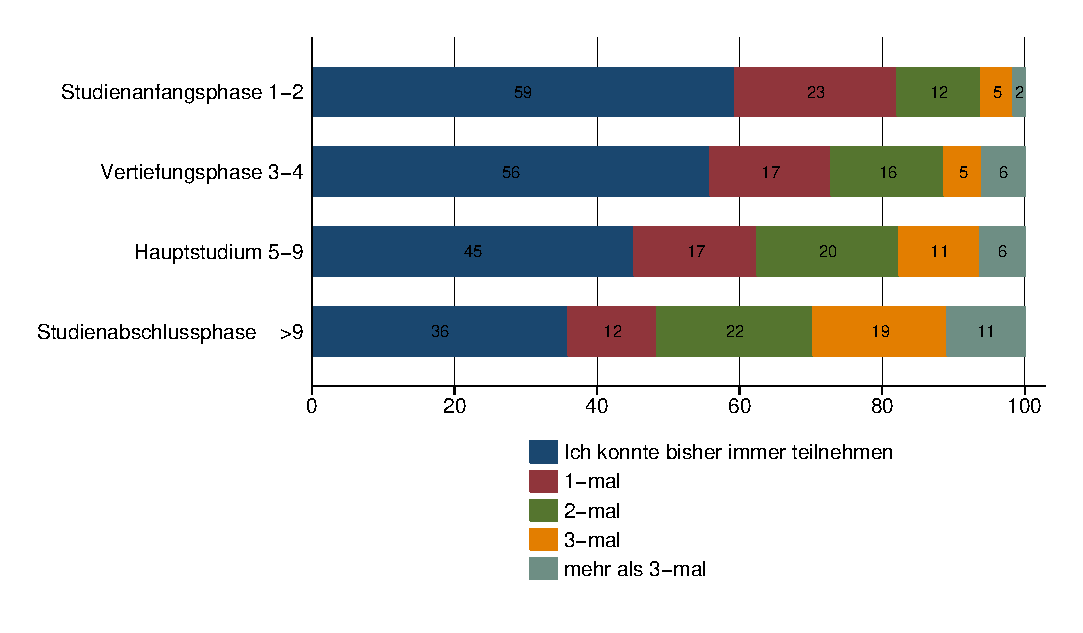
\includegraphics[RemoveGraphicsExtensions={.pdf,PDF}]{image}|
% \end{quote}
%
% \subsection{\plainTeX}
%
% \LaTeX's graphics packages can also be used with \plainTeX.
% The necessary basic \LaTeX\ macros are defined in
% \xfile{miniltx.tex}. This package \xpackage{grfext} also
% relies on it. Example:
%\begin{quote}
%\begin{verbatim}
%\input miniltx.tex\relax
%\def\Gin@driver{pdftex.def}
%\input graphicx.sty\relax
%\input grfext.sty\relax
%\resetatcatcode
%\end{verbatim}
%\end{quote}
%
% \StopEventually{
% }
%
% \section{Implementation}
%
%    \begin{macrocode}
%<*package>
%    \end{macrocode}
%
% \subsection{Relead check and identification}
%    Reload check, especially if the package is not used with \LaTeX.
%    \begin{macrocode}
\begingroup\catcode61\catcode48\catcode32=10\relax%
  \catcode13=5 % ^^M
  \endlinechar=13 %
  \catcode35=6 % #
  \catcode39=12 % '
  \catcode44=12 % ,
  \catcode45=12 % -
  \catcode46=12 % .
  \catcode58=12 % :
  \catcode64=11 % @
  \catcode123=1 % {
  \catcode125=2 % }
  \expandafter\let\expandafter\x\csname ver@grfext.sty\endcsname
  \ifx\x\relax % plain-TeX, first loading
  \else
    \def\empty{}%
    \ifx\x\empty % LaTeX, first loading,
      % variable is initialized, but \ProvidesPackage not yet seen
    \else
      \expandafter\ifx\csname PackageInfo\endcsname\relax
        \def\x#1#2{%
          \immediate\write-1{Package #1 Info: #2.}%
        }%
      \else
        \def\x#1#2{\PackageInfo{#1}{#2, stopped}}%
      \fi
      \x{grfext}{The package is already loaded}%
      \aftergroup\endinput
    \fi
  \fi
\endgroup%
%    \end{macrocode}
%    Package identification:
%    \begin{macrocode}
\begingroup\catcode61\catcode48\catcode32=10\relax%
  \catcode13=5 % ^^M
  \endlinechar=13 %
  \catcode35=6 % #
  \catcode39=12 % '
  \catcode40=12 % (
  \catcode41=12 % )
  \catcode44=12 % ,
  \catcode45=12 % -
  \catcode46=12 % .
  \catcode47=12 % /
  \catcode58=12 % :
  \catcode64=11 % @
  \catcode91=12 % [
  \catcode93=12 % ]
  \catcode123=1 % {
  \catcode125=2 % }
  \expandafter\ifx\csname ProvidesPackage\endcsname\relax
    \def\x#1#2#3[#4]{\endgroup
      \immediate\write-1{Package: #3 #4}%
      \xdef#1{#4}%
    }%
  \else
    \def\x#1#2[#3]{\endgroup
      #2[{#3}]%
      \ifx#1\@undefined
        \xdef#1{#3}%
      \fi
      \ifx#1\relax
        \xdef#1{#3}%
      \fi
    }%
  \fi
\expandafter\x\csname ver@grfext.sty\endcsname
\ProvidesPackage{grfext}%
  [2019/12/03 v1.3 Manage graphics extensions (HO)]%
%    \end{macrocode}
%
% \subsection{Catcodes}
%
%    \begin{macrocode}
\begingroup\catcode61\catcode48\catcode32=10\relax%
  \catcode13=5 % ^^M
  \endlinechar=13 %
  \catcode123=1 % {
  \catcode125=2 % }
  \catcode64=11 % @
  \def\x{\endgroup
    \expandafter\edef\csname grfext@AtEnd\endcsname{%
      \endlinechar=\the\endlinechar\relax
      \catcode13=\the\catcode13\relax
      \catcode32=\the\catcode32\relax
      \catcode35=\the\catcode35\relax
      \catcode61=\the\catcode61\relax
      \catcode64=\the\catcode64\relax
      \catcode123=\the\catcode123\relax
      \catcode125=\the\catcode125\relax
    }%
  }%
\x\catcode61\catcode48\catcode32=10\relax%
\catcode13=5 % ^^M
\endlinechar=13 %
\catcode35=6 % #
\catcode64=11 % @
\catcode123=1 % {
\catcode125=2 % }
\def\TMP@EnsureCode#1#2{%
  \edef\grfext@AtEnd{%
    \grfext@AtEnd
    \catcode#1=\the\catcode#1\relax
  }%
  \catcode#1=#2\relax
}
\TMP@EnsureCode{42}{12}% *
\TMP@EnsureCode{44}{12}% ,
\TMP@EnsureCode{47}{12}% /
\TMP@EnsureCode{58}{12}% :
\TMP@EnsureCode{60}{12}% <
\TMP@EnsureCode{62}{12}% >
\TMP@EnsureCode{91}{12}% [
\TMP@EnsureCode{93}{12}% ]
\edef\grfext@AtEnd{\grfext@AtEnd\noexpand\endinput}
%    \end{macrocode}
%
% \subsection{\plainTeX}
%
%    \begin{macro}{\@expandtwoargs}
%    Requirement is \xfile{miniltx.tex}, but we need also
%    \LaTeX's \cs{@expandtwoargs}.
%    \begin{macrocode}
\@ifundefined{@expandtwoargs}{%
  \def\@expandtwoargs#1#2#3{%
    \edef\reserved@a{\noexpand#1{#2}{#3}}%
    \reserved@a
  }%
}{}
%    \end{macrocode}
%    \end{macro}
%
% \subsection{Add}
%
%    \begin{macro}{\AppendGraphicsExtensions}
%    \begin{macrocode}
\newcommand*{\AppendGraphicsExtensions}{%
  \@ifundefined{Gin@extensions}{%
    \let\Gin@extensions\@empty
  }{}%
  \@ifstar{\grfext@Append\grfext@Check}{\grfext@Append\grfext@@Add}%
}%
%    \end{macrocode}
%    \end{macro}
%    \begin{macro}{\grfext@Append}
%    \begin{macrocode}
\def\grfext@Append#1#2{%
  \let\grfext@Print\@gobble
  \edef\grfext@next{%
    \noexpand\grfext@Add\noexpand#1{%
      \zap@space#2 \@empty
    }{\noexpand\Gin@extensions,}{}%
  }%
  \grfext@next
  \let\grfext@Print\grfext@@Print
  \grfext@Print\AppendGraphicsExtensions
}
%    \end{macrocode}
%    \end{macro}
%
%    \begin{macro}{\PrependGraphicsExtensions}
%    \begin{macrocode}
\newcommand*{\PrependGraphicsExtensions}{%
  \@ifundefined{Gin@extensions}{%
    \let\Gin@extensions\@empty
  }{}%
  \@ifstar{\grfext@Prepend\grfext@Check}{\grfext@Prepend\grfext@@Add}%
}%
%    \end{macrocode}
%    \end{macro}
%    \begin{macro}{\grfext@Prepend}
%    \begin{macrocode}
\def\grfext@Prepend#1#2{%
  \let\grfext@Print\@gobble
  \edef\grfext@next{%
    \noexpand\grfext@Add\noexpand#1{%
      \zap@space#2 \@empty
    }{}{,\noexpand\Gin@extensions}%
  }%
  \grfext@next
  \let\grfext@Print\grfext@@Print
  \grfext@Print\PrependGraphicsExtensions
}
%    \end{macrocode}
%    \end{macro}
%
%    \begin{macro}{\grfext@Add}
%    \begin{macrocode}
\def\grfext@Add#1#2{%
  #1{#2}%
}
%    \end{macrocode}
%    \end{macro}
%    \begin{macro}{\grfext@@Add}
%    \begin{macrocode}
\def\grfext@@Add#1#2#3{%
  \RemoveGraphicsExtensions{#1}%
  \ifx\Gin@extensions\@empty
    \def\Gin@extensions{#1}%
  \else
    \edef\Gin@extensions{#2#1#3}%
  \fi
}
%    \end{macrocode}
%    \end{macro}
%
% \subsection{Check}
%
%    \begin{macro}{\grfext@Check}
%    \begin{macrocode}
\def\grfext@Check#1{%
  \let\grfext@tmp\@empty
  \@for\grfext@ext:=#1\do{%
    \@ifundefined{Gin@rule@\grfext@ext}{%
    }{%
      \ifx\grfext@tmp\@empty
        \let\grfext@tmp\grfext@ext
      \else
        \edef\grfext@tmp{\grfext@tmp,\grfext@ext}%
      \fi
    }%
  }%
  \ifx\grfext@tmp\@empty
    \def\grfext@next##1##2{}%
  \else
    \edef\grfext@next{%
      \noexpand\grfext@@Add{\grfext@tmp}%
    }%
  \fi
  \grfext@next
}
%    \end{macrocode}
%    \end{macro}
%
% \subsection{Remove}
%
%    \begin{macro}{\RemoveGraphicsExtensions}
%    \begin{macrocode}
\newcommand*{\RemoveGraphicsExtensions}[1]{%
  \@ifundefined{Gin@extensions}{%
    \def\Gin@extensions{}%
  }{%
    \edef\grfext@tmp{\zap@space#1 \@empty}%
    \@for\grfext@ext:=\grfext@tmp\do{%
      \def\grfext@next{%
        \let\grfext@tmp\Gin@extensions
        \@expandtwoargs
        \@removeelement\grfext@ext\Gin@extensions\Gin@extensions
        \ifx\grfext@tmp\Gin@extensions
          \let\grfext@next\relax
        \fi
        \grfext@next
      }%
      \grfext@next
    }%
  }%
  \grfext@Print\RemoveGraphicsExtensions
}
%    \end{macrocode}
%    \end{macro}
%
% \subsection{Print}
%
%    \begin{macrocode}
\RequirePackage{infwarerr}[2007/09/09]
%    \end{macrocode}
%
%    \begin{macro}{\PrintGraphicsExtensions}
%    \begin{macrocode}
\def\PrintGraphicsExtensions{%
  \grfext@Print\PrintGraphicsExtensions
}
%    \end{macrocode}
%    \end{macro}
%    \begin{macro}{\grfext@Print}
%    \begin{macrocode}
\def\grfext@Print#1{%
  \@PackageInfo{grfext}{%
    Graphics extension search list:\MessageBreak
    \@ifundefined{Gin@extensions}{%
      <unavailable>%
    }{%
      [\Gin@extensions]%
    }\MessageBreak
    \string#1%
  }%
}
%    \end{macrocode}
%    \end{macro}
%    \begin{macro}{\grfext@@Print}
%    \begin{macrocode}
\let\grfext@@Print\grfext@Print
%    \end{macrocode}
%    \end{macro}
%
% \subsection{Defining options for package \xpackage{graphicx}}
%
%    \begin{macrocode}
\RequirePackage{kvdefinekeys}[2010/03/01]
\kv@define@key{Gin}{AppendGraphicsExtensions}{%
  \AppendGraphicsExtensions{#1}%
}
\kv@define@key{Gin}{AppendGraphicsExtensions*}{%
  \AppendGraphicsExtensions*{#1}%
}
\kv@define@key{Gin}{PrependGraphicsExtensions}{%
  \PrependGraphicsExtensions{#1}%
}
\kv@define@key{Gin}{PrependGraphicsExtensions*}{%
  \PrependGraphicsExtensions*{#1}%
}
\kv@define@key{Gin}{RemoveGraphicsExtensions}{%
  \RemoveGraphicsExtensions{#1}%
}
\kv@define@key{Gin}{PrintGraphicsExtensions}[]{%
  \PrintGraphicsExtensions
}
%    \end{macrocode}
%
%    \begin{macrocode}
\grfext@AtEnd%
%</package>
%    \end{macrocode}
% \section{Installation}
%
% \subsection{Download}
%
% \paragraph{Package.} This package is available on
% CTAN\footnote{\CTANpkg{grfext}}:
% \begin{description}
% \item[\CTAN{macros/latex/contrib/grfext/grfext.dtx}] The source file.
% \item[\CTAN{macros/latex/contrib/grfext/grfext.pdf}] Documentation.
% \end{description}
%
%
% \paragraph{Bundle.} All the packages of the bundle `grfext'
% are also available in a TDS compliant ZIP archive. There
% the packages are already unpacked and the documentation files
% are generated. The files and directories obey the TDS standard.
% \begin{description}
% \item[\CTANinstall{install/macros/latex/contrib/grfext.tds.zip}]
% \end{description}
% \emph{TDS} refers to the standard ``A Directory Structure
% for \TeX\ Files'' (\CTANpkg{tds}). Directories
% with \xfile{texmf} in their name are usually organized this way.
%
% \subsection{Bundle installation}
%
% \paragraph{Unpacking.} Unpack the \xfile{grfext.tds.zip} in the
% TDS tree (also known as \xfile{texmf} tree) of your choice.
% Example (linux):
% \begin{quote}
%   |unzip grfext.tds.zip -d ~/texmf|
% \end{quote}
%
% \subsection{Package installation}
%
% \paragraph{Unpacking.} The \xfile{.dtx} file is a self-extracting
% \docstrip\ archive. The files are extracted by running the
% \xfile{.dtx} through \plainTeX:
% \begin{quote}
%   \verb|tex grfext.dtx|
% \end{quote}
%
% \paragraph{TDS.} Now the different files must be moved into
% the different directories in your installation TDS tree
% (also known as \xfile{texmf} tree):
% \begin{quote}
% \def\t{^^A
% \begin{tabular}{@{}>{\ttfamily}l@{ $\rightarrow$ }>{\ttfamily}l@{}}
%   grfext.sty & tex/latex/grfext/grfext.sty\\
%   grfext.pdf & doc/latex/grfext/grfext.pdf\\
%   grfext.dtx & source/latex/grfext/grfext.dtx\\
% \end{tabular}^^A
% }^^A
% \sbox0{\t}^^A
% \ifdim\wd0>\linewidth
%   \begingroup
%     \advance\linewidth by\leftmargin
%     \advance\linewidth by\rightmargin
%   \edef\x{\endgroup
%     \def\noexpand\lw{\the\linewidth}^^A
%   }\x
%   \def\lwbox{^^A
%     \leavevmode
%     \hbox to \linewidth{^^A
%       \kern-\leftmargin\relax
%       \hss
%       \usebox0
%       \hss
%       \kern-\rightmargin\relax
%     }^^A
%   }^^A
%   \ifdim\wd0>\lw
%     \sbox0{\small\t}^^A
%     \ifdim\wd0>\linewidth
%       \ifdim\wd0>\lw
%         \sbox0{\footnotesize\t}^^A
%         \ifdim\wd0>\linewidth
%           \ifdim\wd0>\lw
%             \sbox0{\scriptsize\t}^^A
%             \ifdim\wd0>\linewidth
%               \ifdim\wd0>\lw
%                 \sbox0{\tiny\t}^^A
%                 \ifdim\wd0>\linewidth
%                   \lwbox
%                 \else
%                   \usebox0
%                 \fi
%               \else
%                 \lwbox
%               \fi
%             \else
%               \usebox0
%             \fi
%           \else
%             \lwbox
%           \fi
%         \else
%           \usebox0
%         \fi
%       \else
%         \lwbox
%       \fi
%     \else
%       \usebox0
%     \fi
%   \else
%     \lwbox
%   \fi
% \else
%   \usebox0
% \fi
% \end{quote}
% If you have a \xfile{docstrip.cfg} that configures and enables \docstrip's
% TDS installing feature, then some files can already be in the right
% place, see the documentation of \docstrip.
%
% \subsection{Refresh file name databases}
%
% If your \TeX~distribution
% (\TeX\,Live, \mikTeX, \dots) relies on file name databases, you must refresh
% these. For example, \TeX\,Live\ users run \verb|texhash| or
% \verb|mktexlsr|.
%
% \subsection{Some details for the interested}
%
% \paragraph{Unpacking with \LaTeX.}
% The \xfile{.dtx} chooses its action depending on the format:
% \begin{description}
% \item[\plainTeX:] Run \docstrip\ and extract the files.
% \item[\LaTeX:] Generate the documentation.
% \end{description}
% If you insist on using \LaTeX\ for \docstrip\ (really,
% \docstrip\ does not need \LaTeX), then inform the autodetect routine
% about your intention:
% \begin{quote}
%   \verb|latex \let\install=y% \iffalse meta-comment
%
% File: grfext.dtx
% Version: 2019/12/03 v1.3
% Info: Manage graphics extensions
%
% Copyright (C)
%    2007, 2010 Heiko Oberdiek
%    2016-2019 Oberdiek Package Support Group
%    https://github.com/ho-tex/grfext/issues
%
% This work may be distributed and/or modified under the
% conditions of the LaTeX Project Public License, either
% version 1.3c of this license or (at your option) any later
% version. This version of this license is in
%    https://www.latex-project.org/lppl/lppl-1-3c.txt
% and the latest version of this license is in
%    https://www.latex-project.org/lppl.txt
% and version 1.3 or later is part of all distributions of
% LaTeX version 2005/12/01 or later.
%
% This work has the LPPL maintenance status "maintained".
%
% The Current Maintainers of this work are
% Heiko Oberdiek and the Oberdiek Package Support Group
% https://github.com/ho-tex/grfext/issues
%
% This work consists of the main source file grfext.dtx
% and the derived files
%    grfext.sty, grfext.pdf, grfext.ins, grfext.drv,
%
% Distribution:
%    CTAN:macros/latex/contrib/grfext/grfext.dtx
%    CTAN:macros/latex/contrib/grfext/grfext.pdf
%
% Unpacking:
%    (a) If grfext.ins is present:
%           tex grfext.ins
%    (b) Without grfext.ins:
%           tex grfext.dtx
%    (c) If you insist on using LaTeX
%           latex \let\install=y% \iffalse meta-comment
%
% File: grfext.dtx
% Version: 2019/12/03 v1.3
% Info: Manage graphics extensions
%
% Copyright (C)
%    2007, 2010 Heiko Oberdiek
%    2016-2019 Oberdiek Package Support Group
%    https://github.com/ho-tex/grfext/issues
%
% This work may be distributed and/or modified under the
% conditions of the LaTeX Project Public License, either
% version 1.3c of this license or (at your option) any later
% version. This version of this license is in
%    https://www.latex-project.org/lppl/lppl-1-3c.txt
% and the latest version of this license is in
%    https://www.latex-project.org/lppl.txt
% and version 1.3 or later is part of all distributions of
% LaTeX version 2005/12/01 or later.
%
% This work has the LPPL maintenance status "maintained".
%
% The Current Maintainers of this work are
% Heiko Oberdiek and the Oberdiek Package Support Group
% https://github.com/ho-tex/grfext/issues
%
% This work consists of the main source file grfext.dtx
% and the derived files
%    grfext.sty, grfext.pdf, grfext.ins, grfext.drv,
%
% Distribution:
%    CTAN:macros/latex/contrib/grfext/grfext.dtx
%    CTAN:macros/latex/contrib/grfext/grfext.pdf
%
% Unpacking:
%    (a) If grfext.ins is present:
%           tex grfext.ins
%    (b) Without grfext.ins:
%           tex grfext.dtx
%    (c) If you insist on using LaTeX
%           latex \let\install=y\input{grfext.dtx}
%        (quote the arguments according to the demands of your shell)
%
% Documentation:
%    (a) If grfext.drv is present:
%           latex grfext.drv
%    (b) Without grfext.drv:
%           latex grfext.dtx; ...
%    The class ltxdoc loads the configuration file ltxdoc.cfg
%    if available. Here you can specify further options, e.g.
%    use A4 as paper format:
%       \PassOptionsToClass{a4paper}{article}
%
%    Programm calls to get the documentation (example):
%       pdflatex grfext.dtx
%       makeindex -s gind.ist grfext.idx
%       pdflatex grfext.dtx
%       makeindex -s gind.ist grfext.idx
%       pdflatex grfext.dtx
%
% Installation:
%    TDS:tex/latex/grfext/grfext.sty
%    TDS:doc/latex/grfext/grfext.pdf
%    TDS:source/latex/grfext/grfext.dtx
%
%<*ignore>
\begingroup
  \catcode123=1 %
  \catcode125=2 %
  \def\x{LaTeX2e}%
\expandafter\endgroup
\ifcase 0\ifx\install y1\fi\expandafter
         \ifx\csname processbatchFile\endcsname\relax\else1\fi
         \ifx\fmtname\x\else 1\fi\relax
\else\csname fi\endcsname
%</ignore>
%<*install>
\input docstrip.tex
\Msg{************************************************************************}
\Msg{* Installation}
\Msg{* Package: grfext 2019/12/03 v1.3 Manage graphics extensions (HO)}
\Msg{************************************************************************}

\keepsilent
\askforoverwritefalse

\let\MetaPrefix\relax
\preamble

This is a generated file.

Project: grfext
Version: 2019/12/03 v1.3

Copyright (C)
   2007, 2010 Heiko Oberdiek
   2016-2019 Oberdiek Package Support Group

This work may be distributed and/or modified under the
conditions of the LaTeX Project Public License, either
version 1.3c of this license or (at your option) any later
version. This version of this license is in
   https://www.latex-project.org/lppl/lppl-1-3c.txt
and the latest version of this license is in
   https://www.latex-project.org/lppl.txt
and version 1.3 or later is part of all distributions of
LaTeX version 2005/12/01 or later.

This work has the LPPL maintenance status "maintained".

The Current Maintainers of this work are
Heiko Oberdiek and the Oberdiek Package Support Group
https://github.com/ho-tex/grfext/issues


This work consists of the main source file grfext.dtx
and the derived files
   grfext.sty, grfext.pdf, grfext.ins, grfext.drv.

\endpreamble
\let\MetaPrefix\DoubleperCent

\generate{%
  \file{grfext.ins}{\from{grfext.dtx}{install}}%
  \file{grfext.drv}{\from{grfext.dtx}{driver}}%
  \usedir{tex/latex/grfext}%
  \file{grfext.sty}{\from{grfext.dtx}{package}}%
%  \usedir{doc/latex/grfext/test}%
%  \file{grfext-test1.tex}{\from{grfext.dtx}{test1}}%
%  \file{grfext-test2.tex}{\from{grfext.dtx}{test2}}%
}

\catcode32=13\relax% active space
\let =\space%
\Msg{************************************************************************}
\Msg{*}
\Msg{* To finish the installation you have to move the following}
\Msg{* file into a directory searched by TeX:}
\Msg{*}
\Msg{*     grfext.sty}
\Msg{*}
\Msg{* To produce the documentation run the file `grfext.drv'}
\Msg{* through LaTeX.}
\Msg{*}
\Msg{* Happy TeXing!}
\Msg{*}
\Msg{************************************************************************}

\endbatchfile
%</install>
%<*ignore>
\fi
%</ignore>
%<*driver>
\NeedsTeXFormat{LaTeX2e}
\ProvidesFile{grfext.drv}%
  [2019/12/03 v1.3 Manage graphics extensions (HO)]%
\documentclass{ltxdoc}
\usepackage{holtxdoc}[2011/11/22]
\begin{document}
  \DocInput{grfext.dtx}%
\end{document}
%</driver>
% \fi
%
%
%
% \GetFileInfo{grfext.drv}
%
% \title{The \xpackage{grfext} package}
% \date{2019/12/03 v1.3}
% \author{Heiko Oberdiek\thanks
% {Please report any issues at \url{https://github.com/ho-tex/grfext/issues}}}
%
% \maketitle
%
% \begin{abstract}
% This package provides macros for adding and reordering
% graphics extensions of package \xpackage{graphics}.
% \end{abstract}
%
% \tableofcontents
%
% \section{Documentation}
%
% \subsection{Introduction}
%
% If you are not familiar with \LaTeX's graphics bundle, please
% read its documentation \xfile{grffile} \cite{graphics}.
% The bundle contains two packages for graphics inclusion:
% \xpackage{graphics} and \xpackage{graphicx}. The first one
% is loaded by the second one that adds a key value interface.
%
% Graphics files are included in both cases by macro
% \cs{includegraphics}. The file name extension can be omitted.
% Then the graphics package goes through a list of known
% extensions until it finds the graphics file. This extension list
% is set by \cs{DeclareGraphicsExtensions}. The previous contents
% of the list is overwritten.
%
% \subsection{User interface}
%
% This package \xpackage{grfext} provides macros that adds entries
% to the list or remove them. The list may be empty or even
% undefined before. It is always defined afterwards, but can
% be empty (especially after removing entries).
%
% \begin{declcs}{AppendGraphicsExtensions} * \M{ext-list}\\
%   \cs{PrependGraphicsExtensions} * \M{ext-list}
% \end{declcs}
% The argument \meta{ext-list} is a comma separated list whose
% entries are file name extensions including the dot.
% But first the entries are removed from
% \xpackage{graphics}' extension list to avoid multiple
% occurences of the same extension.
%
% Then macro \cs{AppendGraphicsExtensions} adds the entries
% after the end of \xpackage{graphics}' list, whereas
% macro \cs{PrependGraphicsExtensions} puts them in front
% of the list.
% The order matters if a graphics file is available in
% different acceptable formats. Then the first extension
% wins.
%
% The star version of these commands only adds an extensions,
% if a specific graphics rule exists for that extension.
%
% \begin{declcs}{RemoveGraphicsExtensions} \M{ext-list}
% \end{declcs}
% All occurences of file extensions in \meta{ext-list} are
% removed from \xpackage{graphics}' extension list.
%
% \subsection{Package loading}
%
% The package does not define any options. It is loaded
% as usual in \LaTeX, e.g.:
% \begin{quote}
%   |\usepackage{grfext}|
% \end{quote}
%
% \begin{declcs}{PrintGraphicsExtensions}
% \end{declcs}
% Macro \cs{PrintGraphicsExtensions} writes the current
% graphics extensions list in the \xfile{.log} file.
% The macros described before do this automatically
% after their operation.
%
% \subsection{Option support for package \xpackage{graphicx}}
%
% Package \xpackage{graphicx} uses the interface of package
% \xpackage{keyval} in order to specify options for
% \cs{includegraphics}. The options can also be set using
% \begin{quote}
%   |\setkeys{Gin}{|\meta{options}|}|
% \end{quote}
% The four user macros with the two star forms are available
% as options in family |Gin| as well:
% \begin{quote}
%   |AppendGraphicsExtensions={|\meta{ext-list}|}|\\
%   |AppendGraphicsExtensions*={|\meta{ext-list}|}|\\
%   |PrependGraphicsExtensions={|\meta{ext-list}|}|\\
%   |PrependGraphicsExtensions*{|\meta{ext-list}|}|\\
%   |RemoveGraphicsExtensions={|\meta{ext-list}|}|\\
%   |PrintGraphicsExtensions|
% \end{quote}
% This makes it easier to locally change the extension list
% for an included graphics, e.g.:
% \begin{quote}
%   |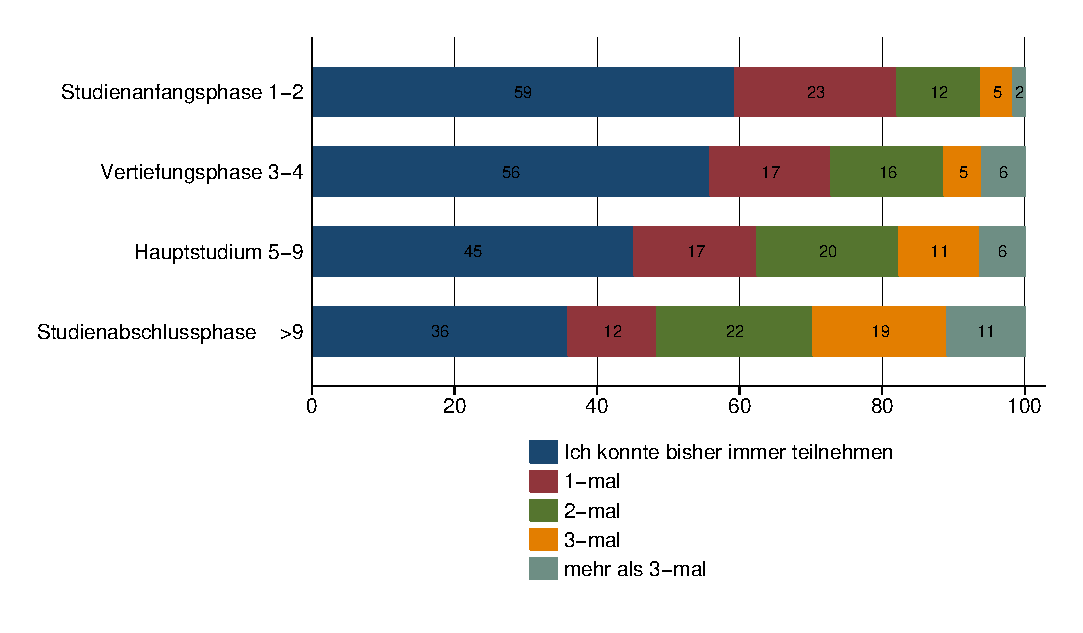
\includegraphics[RemoveGraphicsExtensions={.pdf,PDF}]{image}|
% \end{quote}
%
% \subsection{\plainTeX}
%
% \LaTeX's graphics packages can also be used with \plainTeX.
% The necessary basic \LaTeX\ macros are defined in
% \xfile{miniltx.tex}. This package \xpackage{grfext} also
% relies on it. Example:
%\begin{quote}
%\begin{verbatim}
%\input miniltx.tex\relax
%\def\Gin@driver{pdftex.def}
%\input graphicx.sty\relax
%\input grfext.sty\relax
%\resetatcatcode
%\end{verbatim}
%\end{quote}
%
% \StopEventually{
% }
%
% \section{Implementation}
%
%    \begin{macrocode}
%<*package>
%    \end{macrocode}
%
% \subsection{Relead check and identification}
%    Reload check, especially if the package is not used with \LaTeX.
%    \begin{macrocode}
\begingroup\catcode61\catcode48\catcode32=10\relax%
  \catcode13=5 % ^^M
  \endlinechar=13 %
  \catcode35=6 % #
  \catcode39=12 % '
  \catcode44=12 % ,
  \catcode45=12 % -
  \catcode46=12 % .
  \catcode58=12 % :
  \catcode64=11 % @
  \catcode123=1 % {
  \catcode125=2 % }
  \expandafter\let\expandafter\x\csname ver@grfext.sty\endcsname
  \ifx\x\relax % plain-TeX, first loading
  \else
    \def\empty{}%
    \ifx\x\empty % LaTeX, first loading,
      % variable is initialized, but \ProvidesPackage not yet seen
    \else
      \expandafter\ifx\csname PackageInfo\endcsname\relax
        \def\x#1#2{%
          \immediate\write-1{Package #1 Info: #2.}%
        }%
      \else
        \def\x#1#2{\PackageInfo{#1}{#2, stopped}}%
      \fi
      \x{grfext}{The package is already loaded}%
      \aftergroup\endinput
    \fi
  \fi
\endgroup%
%    \end{macrocode}
%    Package identification:
%    \begin{macrocode}
\begingroup\catcode61\catcode48\catcode32=10\relax%
  \catcode13=5 % ^^M
  \endlinechar=13 %
  \catcode35=6 % #
  \catcode39=12 % '
  \catcode40=12 % (
  \catcode41=12 % )
  \catcode44=12 % ,
  \catcode45=12 % -
  \catcode46=12 % .
  \catcode47=12 % /
  \catcode58=12 % :
  \catcode64=11 % @
  \catcode91=12 % [
  \catcode93=12 % ]
  \catcode123=1 % {
  \catcode125=2 % }
  \expandafter\ifx\csname ProvidesPackage\endcsname\relax
    \def\x#1#2#3[#4]{\endgroup
      \immediate\write-1{Package: #3 #4}%
      \xdef#1{#4}%
    }%
  \else
    \def\x#1#2[#3]{\endgroup
      #2[{#3}]%
      \ifx#1\@undefined
        \xdef#1{#3}%
      \fi
      \ifx#1\relax
        \xdef#1{#3}%
      \fi
    }%
  \fi
\expandafter\x\csname ver@grfext.sty\endcsname
\ProvidesPackage{grfext}%
  [2019/12/03 v1.3 Manage graphics extensions (HO)]%
%    \end{macrocode}
%
% \subsection{Catcodes}
%
%    \begin{macrocode}
\begingroup\catcode61\catcode48\catcode32=10\relax%
  \catcode13=5 % ^^M
  \endlinechar=13 %
  \catcode123=1 % {
  \catcode125=2 % }
  \catcode64=11 % @
  \def\x{\endgroup
    \expandafter\edef\csname grfext@AtEnd\endcsname{%
      \endlinechar=\the\endlinechar\relax
      \catcode13=\the\catcode13\relax
      \catcode32=\the\catcode32\relax
      \catcode35=\the\catcode35\relax
      \catcode61=\the\catcode61\relax
      \catcode64=\the\catcode64\relax
      \catcode123=\the\catcode123\relax
      \catcode125=\the\catcode125\relax
    }%
  }%
\x\catcode61\catcode48\catcode32=10\relax%
\catcode13=5 % ^^M
\endlinechar=13 %
\catcode35=6 % #
\catcode64=11 % @
\catcode123=1 % {
\catcode125=2 % }
\def\TMP@EnsureCode#1#2{%
  \edef\grfext@AtEnd{%
    \grfext@AtEnd
    \catcode#1=\the\catcode#1\relax
  }%
  \catcode#1=#2\relax
}
\TMP@EnsureCode{42}{12}% *
\TMP@EnsureCode{44}{12}% ,
\TMP@EnsureCode{47}{12}% /
\TMP@EnsureCode{58}{12}% :
\TMP@EnsureCode{60}{12}% <
\TMP@EnsureCode{62}{12}% >
\TMP@EnsureCode{91}{12}% [
\TMP@EnsureCode{93}{12}% ]
\edef\grfext@AtEnd{\grfext@AtEnd\noexpand\endinput}
%    \end{macrocode}
%
% \subsection{\plainTeX}
%
%    \begin{macro}{\@expandtwoargs}
%    Requirement is \xfile{miniltx.tex}, but we need also
%    \LaTeX's \cs{@expandtwoargs}.
%    \begin{macrocode}
\@ifundefined{@expandtwoargs}{%
  \def\@expandtwoargs#1#2#3{%
    \edef\reserved@a{\noexpand#1{#2}{#3}}%
    \reserved@a
  }%
}{}
%    \end{macrocode}
%    \end{macro}
%
% \subsection{Add}
%
%    \begin{macro}{\AppendGraphicsExtensions}
%    \begin{macrocode}
\newcommand*{\AppendGraphicsExtensions}{%
  \@ifundefined{Gin@extensions}{%
    \let\Gin@extensions\@empty
  }{}%
  \@ifstar{\grfext@Append\grfext@Check}{\grfext@Append\grfext@@Add}%
}%
%    \end{macrocode}
%    \end{macro}
%    \begin{macro}{\grfext@Append}
%    \begin{macrocode}
\def\grfext@Append#1#2{%
  \let\grfext@Print\@gobble
  \edef\grfext@next{%
    \noexpand\grfext@Add\noexpand#1{%
      \zap@space#2 \@empty
    }{\noexpand\Gin@extensions,}{}%
  }%
  \grfext@next
  \let\grfext@Print\grfext@@Print
  \grfext@Print\AppendGraphicsExtensions
}
%    \end{macrocode}
%    \end{macro}
%
%    \begin{macro}{\PrependGraphicsExtensions}
%    \begin{macrocode}
\newcommand*{\PrependGraphicsExtensions}{%
  \@ifundefined{Gin@extensions}{%
    \let\Gin@extensions\@empty
  }{}%
  \@ifstar{\grfext@Prepend\grfext@Check}{\grfext@Prepend\grfext@@Add}%
}%
%    \end{macrocode}
%    \end{macro}
%    \begin{macro}{\grfext@Prepend}
%    \begin{macrocode}
\def\grfext@Prepend#1#2{%
  \let\grfext@Print\@gobble
  \edef\grfext@next{%
    \noexpand\grfext@Add\noexpand#1{%
      \zap@space#2 \@empty
    }{}{,\noexpand\Gin@extensions}%
  }%
  \grfext@next
  \let\grfext@Print\grfext@@Print
  \grfext@Print\PrependGraphicsExtensions
}
%    \end{macrocode}
%    \end{macro}
%
%    \begin{macro}{\grfext@Add}
%    \begin{macrocode}
\def\grfext@Add#1#2{%
  #1{#2}%
}
%    \end{macrocode}
%    \end{macro}
%    \begin{macro}{\grfext@@Add}
%    \begin{macrocode}
\def\grfext@@Add#1#2#3{%
  \RemoveGraphicsExtensions{#1}%
  \ifx\Gin@extensions\@empty
    \def\Gin@extensions{#1}%
  \else
    \edef\Gin@extensions{#2#1#3}%
  \fi
}
%    \end{macrocode}
%    \end{macro}
%
% \subsection{Check}
%
%    \begin{macro}{\grfext@Check}
%    \begin{macrocode}
\def\grfext@Check#1{%
  \let\grfext@tmp\@empty
  \@for\grfext@ext:=#1\do{%
    \@ifundefined{Gin@rule@\grfext@ext}{%
    }{%
      \ifx\grfext@tmp\@empty
        \let\grfext@tmp\grfext@ext
      \else
        \edef\grfext@tmp{\grfext@tmp,\grfext@ext}%
      \fi
    }%
  }%
  \ifx\grfext@tmp\@empty
    \def\grfext@next##1##2{}%
  \else
    \edef\grfext@next{%
      \noexpand\grfext@@Add{\grfext@tmp}%
    }%
  \fi
  \grfext@next
}
%    \end{macrocode}
%    \end{macro}
%
% \subsection{Remove}
%
%    \begin{macro}{\RemoveGraphicsExtensions}
%    \begin{macrocode}
\newcommand*{\RemoveGraphicsExtensions}[1]{%
  \@ifundefined{Gin@extensions}{%
    \def\Gin@extensions{}%
  }{%
    \edef\grfext@tmp{\zap@space#1 \@empty}%
    \@for\grfext@ext:=\grfext@tmp\do{%
      \def\grfext@next{%
        \let\grfext@tmp\Gin@extensions
        \@expandtwoargs
        \@removeelement\grfext@ext\Gin@extensions\Gin@extensions
        \ifx\grfext@tmp\Gin@extensions
          \let\grfext@next\relax
        \fi
        \grfext@next
      }%
      \grfext@next
    }%
  }%
  \grfext@Print\RemoveGraphicsExtensions
}
%    \end{macrocode}
%    \end{macro}
%
% \subsection{Print}
%
%    \begin{macrocode}
\RequirePackage{infwarerr}[2007/09/09]
%    \end{macrocode}
%
%    \begin{macro}{\PrintGraphicsExtensions}
%    \begin{macrocode}
\def\PrintGraphicsExtensions{%
  \grfext@Print\PrintGraphicsExtensions
}
%    \end{macrocode}
%    \end{macro}
%    \begin{macro}{\grfext@Print}
%    \begin{macrocode}
\def\grfext@Print#1{%
  \@PackageInfo{grfext}{%
    Graphics extension search list:\MessageBreak
    \@ifundefined{Gin@extensions}{%
      <unavailable>%
    }{%
      [\Gin@extensions]%
    }\MessageBreak
    \string#1%
  }%
}
%    \end{macrocode}
%    \end{macro}
%    \begin{macro}{\grfext@@Print}
%    \begin{macrocode}
\let\grfext@@Print\grfext@Print
%    \end{macrocode}
%    \end{macro}
%
% \subsection{Defining options for package \xpackage{graphicx}}
%
%    \begin{macrocode}
\RequirePackage{kvdefinekeys}[2010/03/01]
\kv@define@key{Gin}{AppendGraphicsExtensions}{%
  \AppendGraphicsExtensions{#1}%
}
\kv@define@key{Gin}{AppendGraphicsExtensions*}{%
  \AppendGraphicsExtensions*{#1}%
}
\kv@define@key{Gin}{PrependGraphicsExtensions}{%
  \PrependGraphicsExtensions{#1}%
}
\kv@define@key{Gin}{PrependGraphicsExtensions*}{%
  \PrependGraphicsExtensions*{#1}%
}
\kv@define@key{Gin}{RemoveGraphicsExtensions}{%
  \RemoveGraphicsExtensions{#1}%
}
\kv@define@key{Gin}{PrintGraphicsExtensions}[]{%
  \PrintGraphicsExtensions
}
%    \end{macrocode}
%
%    \begin{macrocode}
\grfext@AtEnd%
%</package>
%    \end{macrocode}
% \section{Installation}
%
% \subsection{Download}
%
% \paragraph{Package.} This package is available on
% CTAN\footnote{\CTANpkg{grfext}}:
% \begin{description}
% \item[\CTAN{macros/latex/contrib/grfext/grfext.dtx}] The source file.
% \item[\CTAN{macros/latex/contrib/grfext/grfext.pdf}] Documentation.
% \end{description}
%
%
% \paragraph{Bundle.} All the packages of the bundle `grfext'
% are also available in a TDS compliant ZIP archive. There
% the packages are already unpacked and the documentation files
% are generated. The files and directories obey the TDS standard.
% \begin{description}
% \item[\CTANinstall{install/macros/latex/contrib/grfext.tds.zip}]
% \end{description}
% \emph{TDS} refers to the standard ``A Directory Structure
% for \TeX\ Files'' (\CTANpkg{tds}). Directories
% with \xfile{texmf} in their name are usually organized this way.
%
% \subsection{Bundle installation}
%
% \paragraph{Unpacking.} Unpack the \xfile{grfext.tds.zip} in the
% TDS tree (also known as \xfile{texmf} tree) of your choice.
% Example (linux):
% \begin{quote}
%   |unzip grfext.tds.zip -d ~/texmf|
% \end{quote}
%
% \subsection{Package installation}
%
% \paragraph{Unpacking.} The \xfile{.dtx} file is a self-extracting
% \docstrip\ archive. The files are extracted by running the
% \xfile{.dtx} through \plainTeX:
% \begin{quote}
%   \verb|tex grfext.dtx|
% \end{quote}
%
% \paragraph{TDS.} Now the different files must be moved into
% the different directories in your installation TDS tree
% (also known as \xfile{texmf} tree):
% \begin{quote}
% \def\t{^^A
% \begin{tabular}{@{}>{\ttfamily}l@{ $\rightarrow$ }>{\ttfamily}l@{}}
%   grfext.sty & tex/latex/grfext/grfext.sty\\
%   grfext.pdf & doc/latex/grfext/grfext.pdf\\
%   grfext.dtx & source/latex/grfext/grfext.dtx\\
% \end{tabular}^^A
% }^^A
% \sbox0{\t}^^A
% \ifdim\wd0>\linewidth
%   \begingroup
%     \advance\linewidth by\leftmargin
%     \advance\linewidth by\rightmargin
%   \edef\x{\endgroup
%     \def\noexpand\lw{\the\linewidth}^^A
%   }\x
%   \def\lwbox{^^A
%     \leavevmode
%     \hbox to \linewidth{^^A
%       \kern-\leftmargin\relax
%       \hss
%       \usebox0
%       \hss
%       \kern-\rightmargin\relax
%     }^^A
%   }^^A
%   \ifdim\wd0>\lw
%     \sbox0{\small\t}^^A
%     \ifdim\wd0>\linewidth
%       \ifdim\wd0>\lw
%         \sbox0{\footnotesize\t}^^A
%         \ifdim\wd0>\linewidth
%           \ifdim\wd0>\lw
%             \sbox0{\scriptsize\t}^^A
%             \ifdim\wd0>\linewidth
%               \ifdim\wd0>\lw
%                 \sbox0{\tiny\t}^^A
%                 \ifdim\wd0>\linewidth
%                   \lwbox
%                 \else
%                   \usebox0
%                 \fi
%               \else
%                 \lwbox
%               \fi
%             \else
%               \usebox0
%             \fi
%           \else
%             \lwbox
%           \fi
%         \else
%           \usebox0
%         \fi
%       \else
%         \lwbox
%       \fi
%     \else
%       \usebox0
%     \fi
%   \else
%     \lwbox
%   \fi
% \else
%   \usebox0
% \fi
% \end{quote}
% If you have a \xfile{docstrip.cfg} that configures and enables \docstrip's
% TDS installing feature, then some files can already be in the right
% place, see the documentation of \docstrip.
%
% \subsection{Refresh file name databases}
%
% If your \TeX~distribution
% (\TeX\,Live, \mikTeX, \dots) relies on file name databases, you must refresh
% these. For example, \TeX\,Live\ users run \verb|texhash| or
% \verb|mktexlsr|.
%
% \subsection{Some details for the interested}
%
% \paragraph{Unpacking with \LaTeX.}
% The \xfile{.dtx} chooses its action depending on the format:
% \begin{description}
% \item[\plainTeX:] Run \docstrip\ and extract the files.
% \item[\LaTeX:] Generate the documentation.
% \end{description}
% If you insist on using \LaTeX\ for \docstrip\ (really,
% \docstrip\ does not need \LaTeX), then inform the autodetect routine
% about your intention:
% \begin{quote}
%   \verb|latex \let\install=y\input{grfext.dtx}|
% \end{quote}
% Do not forget to quote the argument according to the demands
% of your shell.
%
% \paragraph{Generating the documentation.}
% You can use both the \xfile{.dtx} or the \xfile{.drv} to generate
% the documentation. The process can be configured by the
% configuration file \xfile{ltxdoc.cfg}. For instance, put this
% line into this file, if you want to have A4 as paper format:
% \begin{quote}
%   \verb|\PassOptionsToClass{a4paper}{article}|
% \end{quote}
% An example follows how to generate the
% documentation with pdf\LaTeX:
% \begin{quote}
%\begin{verbatim}
%pdflatex grfext.dtx
%makeindex -s gind.ist grfext.idx
%pdflatex grfext.dtx
%makeindex -s gind.ist grfext.idx
%pdflatex grfext.dtx
%\end{verbatim}
% \end{quote}
%
% \begin{thebibliography}{9}
%
% \bibitem{graphics}
%   David Carlisle, Sebastian Rahtz: \textit{The \xpackage{graphics} package};
%   2006/02/20 v1.0o;
%   \CTAN{macros/latex/required/graphics/graphics.dtx}.
%
% \end{thebibliography}
%
% \begin{History}
%   \begin{Version}{2007/09/30 v1.0}
%   \item
%     First public version.
%   \end{Version}
%   \begin{Version}{2010/08/19 v1.1}
%   \item
%     User macros are also made available as keyval options for
%     package \xpackage{graphicx}.
%   \end{Version}
%   \begin{Version}{2016/05/16 v1.2}
%   \item
%     Documentation updates.
%   \end{Version}
%   \begin{Version}{2019/12/03 v1.3}
%   \item
%     Documentation updates.
%   \end{Version}
% \end{History}
%
% \PrintIndex
%
% \Finale
\endinput

%        (quote the arguments according to the demands of your shell)
%
% Documentation:
%    (a) If grfext.drv is present:
%           latex grfext.drv
%    (b) Without grfext.drv:
%           latex grfext.dtx; ...
%    The class ltxdoc loads the configuration file ltxdoc.cfg
%    if available. Here you can specify further options, e.g.
%    use A4 as paper format:
%       \PassOptionsToClass{a4paper}{article}
%
%    Programm calls to get the documentation (example):
%       pdflatex grfext.dtx
%       makeindex -s gind.ist grfext.idx
%       pdflatex grfext.dtx
%       makeindex -s gind.ist grfext.idx
%       pdflatex grfext.dtx
%
% Installation:
%    TDS:tex/latex/grfext/grfext.sty
%    TDS:doc/latex/grfext/grfext.pdf
%    TDS:source/latex/grfext/grfext.dtx
%
%<*ignore>
\begingroup
  \catcode123=1 %
  \catcode125=2 %
  \def\x{LaTeX2e}%
\expandafter\endgroup
\ifcase 0\ifx\install y1\fi\expandafter
         \ifx\csname processbatchFile\endcsname\relax\else1\fi
         \ifx\fmtname\x\else 1\fi\relax
\else\csname fi\endcsname
%</ignore>
%<*install>
\input docstrip.tex
\Msg{************************************************************************}
\Msg{* Installation}
\Msg{* Package: grfext 2019/12/03 v1.3 Manage graphics extensions (HO)}
\Msg{************************************************************************}

\keepsilent
\askforoverwritefalse

\let\MetaPrefix\relax
\preamble

This is a generated file.

Project: grfext
Version: 2019/12/03 v1.3

Copyright (C)
   2007, 2010 Heiko Oberdiek
   2016-2019 Oberdiek Package Support Group

This work may be distributed and/or modified under the
conditions of the LaTeX Project Public License, either
version 1.3c of this license or (at your option) any later
version. This version of this license is in
   https://www.latex-project.org/lppl/lppl-1-3c.txt
and the latest version of this license is in
   https://www.latex-project.org/lppl.txt
and version 1.3 or later is part of all distributions of
LaTeX version 2005/12/01 or later.

This work has the LPPL maintenance status "maintained".

The Current Maintainers of this work are
Heiko Oberdiek and the Oberdiek Package Support Group
https://github.com/ho-tex/grfext/issues


This work consists of the main source file grfext.dtx
and the derived files
   grfext.sty, grfext.pdf, grfext.ins, grfext.drv.

\endpreamble
\let\MetaPrefix\DoubleperCent

\generate{%
  \file{grfext.ins}{\from{grfext.dtx}{install}}%
  \file{grfext.drv}{\from{grfext.dtx}{driver}}%
  \usedir{tex/latex/grfext}%
  \file{grfext.sty}{\from{grfext.dtx}{package}}%
%  \usedir{doc/latex/grfext/test}%
%  \file{grfext-test1.tex}{\from{grfext.dtx}{test1}}%
%  \file{grfext-test2.tex}{\from{grfext.dtx}{test2}}%
}

\catcode32=13\relax% active space
\let =\space%
\Msg{************************************************************************}
\Msg{*}
\Msg{* To finish the installation you have to move the following}
\Msg{* file into a directory searched by TeX:}
\Msg{*}
\Msg{*     grfext.sty}
\Msg{*}
\Msg{* To produce the documentation run the file `grfext.drv'}
\Msg{* through LaTeX.}
\Msg{*}
\Msg{* Happy TeXing!}
\Msg{*}
\Msg{************************************************************************}

\endbatchfile
%</install>
%<*ignore>
\fi
%</ignore>
%<*driver>
\NeedsTeXFormat{LaTeX2e}
\ProvidesFile{grfext.drv}%
  [2019/12/03 v1.3 Manage graphics extensions (HO)]%
\documentclass{ltxdoc}
\usepackage{holtxdoc}[2011/11/22]
\begin{document}
  \DocInput{grfext.dtx}%
\end{document}
%</driver>
% \fi
%
%
%
% \GetFileInfo{grfext.drv}
%
% \title{The \xpackage{grfext} package}
% \date{2019/12/03 v1.3}
% \author{Heiko Oberdiek\thanks
% {Please report any issues at \url{https://github.com/ho-tex/grfext/issues}}}
%
% \maketitle
%
% \begin{abstract}
% This package provides macros for adding and reordering
% graphics extensions of package \xpackage{graphics}.
% \end{abstract}
%
% \tableofcontents
%
% \section{Documentation}
%
% \subsection{Introduction}
%
% If you are not familiar with \LaTeX's graphics bundle, please
% read its documentation \xfile{grffile} \cite{graphics}.
% The bundle contains two packages for graphics inclusion:
% \xpackage{graphics} and \xpackage{graphicx}. The first one
% is loaded by the second one that adds a key value interface.
%
% Graphics files are included in both cases by macro
% \cs{includegraphics}. The file name extension can be omitted.
% Then the graphics package goes through a list of known
% extensions until it finds the graphics file. This extension list
% is set by \cs{DeclareGraphicsExtensions}. The previous contents
% of the list is overwritten.
%
% \subsection{User interface}
%
% This package \xpackage{grfext} provides macros that adds entries
% to the list or remove them. The list may be empty or even
% undefined before. It is always defined afterwards, but can
% be empty (especially after removing entries).
%
% \begin{declcs}{AppendGraphicsExtensions} * \M{ext-list}\\
%   \cs{PrependGraphicsExtensions} * \M{ext-list}
% \end{declcs}
% The argument \meta{ext-list} is a comma separated list whose
% entries are file name extensions including the dot.
% But first the entries are removed from
% \xpackage{graphics}' extension list to avoid multiple
% occurences of the same extension.
%
% Then macro \cs{AppendGraphicsExtensions} adds the entries
% after the end of \xpackage{graphics}' list, whereas
% macro \cs{PrependGraphicsExtensions} puts them in front
% of the list.
% The order matters if a graphics file is available in
% different acceptable formats. Then the first extension
% wins.
%
% The star version of these commands only adds an extensions,
% if a specific graphics rule exists for that extension.
%
% \begin{declcs}{RemoveGraphicsExtensions} \M{ext-list}
% \end{declcs}
% All occurences of file extensions in \meta{ext-list} are
% removed from \xpackage{graphics}' extension list.
%
% \subsection{Package loading}
%
% The package does not define any options. It is loaded
% as usual in \LaTeX, e.g.:
% \begin{quote}
%   |\usepackage{grfext}|
% \end{quote}
%
% \begin{declcs}{PrintGraphicsExtensions}
% \end{declcs}
% Macro \cs{PrintGraphicsExtensions} writes the current
% graphics extensions list in the \xfile{.log} file.
% The macros described before do this automatically
% after their operation.
%
% \subsection{Option support for package \xpackage{graphicx}}
%
% Package \xpackage{graphicx} uses the interface of package
% \xpackage{keyval} in order to specify options for
% \cs{includegraphics}. The options can also be set using
% \begin{quote}
%   |\setkeys{Gin}{|\meta{options}|}|
% \end{quote}
% The four user macros with the two star forms are available
% as options in family |Gin| as well:
% \begin{quote}
%   |AppendGraphicsExtensions={|\meta{ext-list}|}|\\
%   |AppendGraphicsExtensions*={|\meta{ext-list}|}|\\
%   |PrependGraphicsExtensions={|\meta{ext-list}|}|\\
%   |PrependGraphicsExtensions*{|\meta{ext-list}|}|\\
%   |RemoveGraphicsExtensions={|\meta{ext-list}|}|\\
%   |PrintGraphicsExtensions|
% \end{quote}
% This makes it easier to locally change the extension list
% for an included graphics, e.g.:
% \begin{quote}
%   |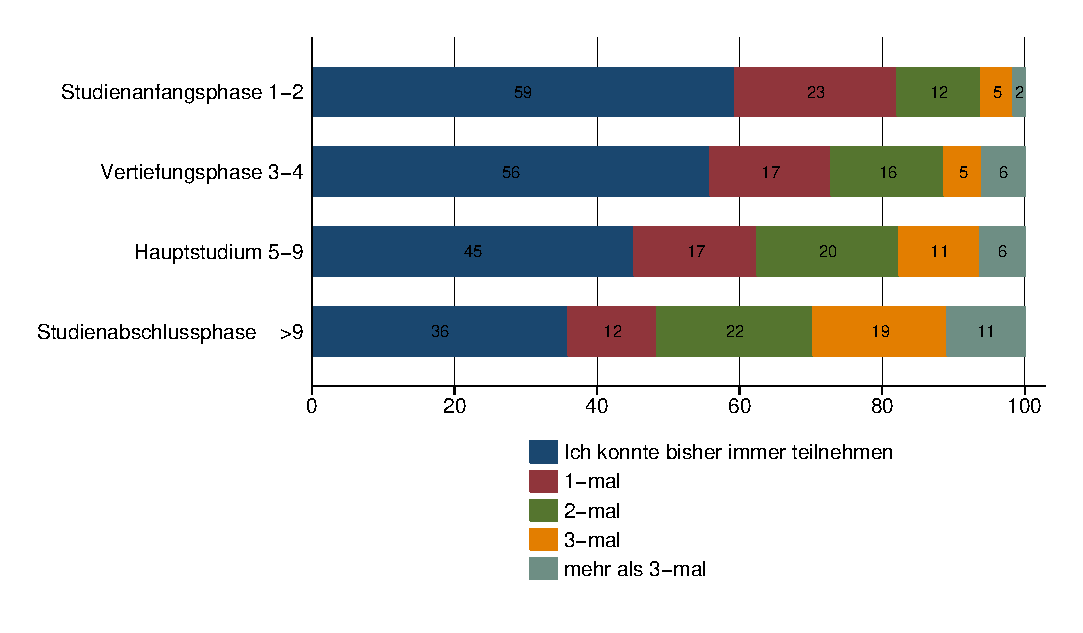
\includegraphics[RemoveGraphicsExtensions={.pdf,PDF}]{image}|
% \end{quote}
%
% \subsection{\plainTeX}
%
% \LaTeX's graphics packages can also be used with \plainTeX.
% The necessary basic \LaTeX\ macros are defined in
% \xfile{miniltx.tex}. This package \xpackage{grfext} also
% relies on it. Example:
%\begin{quote}
%\begin{verbatim}
%\input miniltx.tex\relax
%\def\Gin@driver{pdftex.def}
%\input graphicx.sty\relax
%\input grfext.sty\relax
%\resetatcatcode
%\end{verbatim}
%\end{quote}
%
% \StopEventually{
% }
%
% \section{Implementation}
%
%    \begin{macrocode}
%<*package>
%    \end{macrocode}
%
% \subsection{Relead check and identification}
%    Reload check, especially if the package is not used with \LaTeX.
%    \begin{macrocode}
\begingroup\catcode61\catcode48\catcode32=10\relax%
  \catcode13=5 % ^^M
  \endlinechar=13 %
  \catcode35=6 % #
  \catcode39=12 % '
  \catcode44=12 % ,
  \catcode45=12 % -
  \catcode46=12 % .
  \catcode58=12 % :
  \catcode64=11 % @
  \catcode123=1 % {
  \catcode125=2 % }
  \expandafter\let\expandafter\x\csname ver@grfext.sty\endcsname
  \ifx\x\relax % plain-TeX, first loading
  \else
    \def\empty{}%
    \ifx\x\empty % LaTeX, first loading,
      % variable is initialized, but \ProvidesPackage not yet seen
    \else
      \expandafter\ifx\csname PackageInfo\endcsname\relax
        \def\x#1#2{%
          \immediate\write-1{Package #1 Info: #2.}%
        }%
      \else
        \def\x#1#2{\PackageInfo{#1}{#2, stopped}}%
      \fi
      \x{grfext}{The package is already loaded}%
      \aftergroup\endinput
    \fi
  \fi
\endgroup%
%    \end{macrocode}
%    Package identification:
%    \begin{macrocode}
\begingroup\catcode61\catcode48\catcode32=10\relax%
  \catcode13=5 % ^^M
  \endlinechar=13 %
  \catcode35=6 % #
  \catcode39=12 % '
  \catcode40=12 % (
  \catcode41=12 % )
  \catcode44=12 % ,
  \catcode45=12 % -
  \catcode46=12 % .
  \catcode47=12 % /
  \catcode58=12 % :
  \catcode64=11 % @
  \catcode91=12 % [
  \catcode93=12 % ]
  \catcode123=1 % {
  \catcode125=2 % }
  \expandafter\ifx\csname ProvidesPackage\endcsname\relax
    \def\x#1#2#3[#4]{\endgroup
      \immediate\write-1{Package: #3 #4}%
      \xdef#1{#4}%
    }%
  \else
    \def\x#1#2[#3]{\endgroup
      #2[{#3}]%
      \ifx#1\@undefined
        \xdef#1{#3}%
      \fi
      \ifx#1\relax
        \xdef#1{#3}%
      \fi
    }%
  \fi
\expandafter\x\csname ver@grfext.sty\endcsname
\ProvidesPackage{grfext}%
  [2019/12/03 v1.3 Manage graphics extensions (HO)]%
%    \end{macrocode}
%
% \subsection{Catcodes}
%
%    \begin{macrocode}
\begingroup\catcode61\catcode48\catcode32=10\relax%
  \catcode13=5 % ^^M
  \endlinechar=13 %
  \catcode123=1 % {
  \catcode125=2 % }
  \catcode64=11 % @
  \def\x{\endgroup
    \expandafter\edef\csname grfext@AtEnd\endcsname{%
      \endlinechar=\the\endlinechar\relax
      \catcode13=\the\catcode13\relax
      \catcode32=\the\catcode32\relax
      \catcode35=\the\catcode35\relax
      \catcode61=\the\catcode61\relax
      \catcode64=\the\catcode64\relax
      \catcode123=\the\catcode123\relax
      \catcode125=\the\catcode125\relax
    }%
  }%
\x\catcode61\catcode48\catcode32=10\relax%
\catcode13=5 % ^^M
\endlinechar=13 %
\catcode35=6 % #
\catcode64=11 % @
\catcode123=1 % {
\catcode125=2 % }
\def\TMP@EnsureCode#1#2{%
  \edef\grfext@AtEnd{%
    \grfext@AtEnd
    \catcode#1=\the\catcode#1\relax
  }%
  \catcode#1=#2\relax
}
\TMP@EnsureCode{42}{12}% *
\TMP@EnsureCode{44}{12}% ,
\TMP@EnsureCode{47}{12}% /
\TMP@EnsureCode{58}{12}% :
\TMP@EnsureCode{60}{12}% <
\TMP@EnsureCode{62}{12}% >
\TMP@EnsureCode{91}{12}% [
\TMP@EnsureCode{93}{12}% ]
\edef\grfext@AtEnd{\grfext@AtEnd\noexpand\endinput}
%    \end{macrocode}
%
% \subsection{\plainTeX}
%
%    \begin{macro}{\@expandtwoargs}
%    Requirement is \xfile{miniltx.tex}, but we need also
%    \LaTeX's \cs{@expandtwoargs}.
%    \begin{macrocode}
\@ifundefined{@expandtwoargs}{%
  \def\@expandtwoargs#1#2#3{%
    \edef\reserved@a{\noexpand#1{#2}{#3}}%
    \reserved@a
  }%
}{}
%    \end{macrocode}
%    \end{macro}
%
% \subsection{Add}
%
%    \begin{macro}{\AppendGraphicsExtensions}
%    \begin{macrocode}
\newcommand*{\AppendGraphicsExtensions}{%
  \@ifundefined{Gin@extensions}{%
    \let\Gin@extensions\@empty
  }{}%
  \@ifstar{\grfext@Append\grfext@Check}{\grfext@Append\grfext@@Add}%
}%
%    \end{macrocode}
%    \end{macro}
%    \begin{macro}{\grfext@Append}
%    \begin{macrocode}
\def\grfext@Append#1#2{%
  \let\grfext@Print\@gobble
  \edef\grfext@next{%
    \noexpand\grfext@Add\noexpand#1{%
      \zap@space#2 \@empty
    }{\noexpand\Gin@extensions,}{}%
  }%
  \grfext@next
  \let\grfext@Print\grfext@@Print
  \grfext@Print\AppendGraphicsExtensions
}
%    \end{macrocode}
%    \end{macro}
%
%    \begin{macro}{\PrependGraphicsExtensions}
%    \begin{macrocode}
\newcommand*{\PrependGraphicsExtensions}{%
  \@ifundefined{Gin@extensions}{%
    \let\Gin@extensions\@empty
  }{}%
  \@ifstar{\grfext@Prepend\grfext@Check}{\grfext@Prepend\grfext@@Add}%
}%
%    \end{macrocode}
%    \end{macro}
%    \begin{macro}{\grfext@Prepend}
%    \begin{macrocode}
\def\grfext@Prepend#1#2{%
  \let\grfext@Print\@gobble
  \edef\grfext@next{%
    \noexpand\grfext@Add\noexpand#1{%
      \zap@space#2 \@empty
    }{}{,\noexpand\Gin@extensions}%
  }%
  \grfext@next
  \let\grfext@Print\grfext@@Print
  \grfext@Print\PrependGraphicsExtensions
}
%    \end{macrocode}
%    \end{macro}
%
%    \begin{macro}{\grfext@Add}
%    \begin{macrocode}
\def\grfext@Add#1#2{%
  #1{#2}%
}
%    \end{macrocode}
%    \end{macro}
%    \begin{macro}{\grfext@@Add}
%    \begin{macrocode}
\def\grfext@@Add#1#2#3{%
  \RemoveGraphicsExtensions{#1}%
  \ifx\Gin@extensions\@empty
    \def\Gin@extensions{#1}%
  \else
    \edef\Gin@extensions{#2#1#3}%
  \fi
}
%    \end{macrocode}
%    \end{macro}
%
% \subsection{Check}
%
%    \begin{macro}{\grfext@Check}
%    \begin{macrocode}
\def\grfext@Check#1{%
  \let\grfext@tmp\@empty
  \@for\grfext@ext:=#1\do{%
    \@ifundefined{Gin@rule@\grfext@ext}{%
    }{%
      \ifx\grfext@tmp\@empty
        \let\grfext@tmp\grfext@ext
      \else
        \edef\grfext@tmp{\grfext@tmp,\grfext@ext}%
      \fi
    }%
  }%
  \ifx\grfext@tmp\@empty
    \def\grfext@next##1##2{}%
  \else
    \edef\grfext@next{%
      \noexpand\grfext@@Add{\grfext@tmp}%
    }%
  \fi
  \grfext@next
}
%    \end{macrocode}
%    \end{macro}
%
% \subsection{Remove}
%
%    \begin{macro}{\RemoveGraphicsExtensions}
%    \begin{macrocode}
\newcommand*{\RemoveGraphicsExtensions}[1]{%
  \@ifundefined{Gin@extensions}{%
    \def\Gin@extensions{}%
  }{%
    \edef\grfext@tmp{\zap@space#1 \@empty}%
    \@for\grfext@ext:=\grfext@tmp\do{%
      \def\grfext@next{%
        \let\grfext@tmp\Gin@extensions
        \@expandtwoargs
        \@removeelement\grfext@ext\Gin@extensions\Gin@extensions
        \ifx\grfext@tmp\Gin@extensions
          \let\grfext@next\relax
        \fi
        \grfext@next
      }%
      \grfext@next
    }%
  }%
  \grfext@Print\RemoveGraphicsExtensions
}
%    \end{macrocode}
%    \end{macro}
%
% \subsection{Print}
%
%    \begin{macrocode}
\RequirePackage{infwarerr}[2007/09/09]
%    \end{macrocode}
%
%    \begin{macro}{\PrintGraphicsExtensions}
%    \begin{macrocode}
\def\PrintGraphicsExtensions{%
  \grfext@Print\PrintGraphicsExtensions
}
%    \end{macrocode}
%    \end{macro}
%    \begin{macro}{\grfext@Print}
%    \begin{macrocode}
\def\grfext@Print#1{%
  \@PackageInfo{grfext}{%
    Graphics extension search list:\MessageBreak
    \@ifundefined{Gin@extensions}{%
      <unavailable>%
    }{%
      [\Gin@extensions]%
    }\MessageBreak
    \string#1%
  }%
}
%    \end{macrocode}
%    \end{macro}
%    \begin{macro}{\grfext@@Print}
%    \begin{macrocode}
\let\grfext@@Print\grfext@Print
%    \end{macrocode}
%    \end{macro}
%
% \subsection{Defining options for package \xpackage{graphicx}}
%
%    \begin{macrocode}
\RequirePackage{kvdefinekeys}[2010/03/01]
\kv@define@key{Gin}{AppendGraphicsExtensions}{%
  \AppendGraphicsExtensions{#1}%
}
\kv@define@key{Gin}{AppendGraphicsExtensions*}{%
  \AppendGraphicsExtensions*{#1}%
}
\kv@define@key{Gin}{PrependGraphicsExtensions}{%
  \PrependGraphicsExtensions{#1}%
}
\kv@define@key{Gin}{PrependGraphicsExtensions*}{%
  \PrependGraphicsExtensions*{#1}%
}
\kv@define@key{Gin}{RemoveGraphicsExtensions}{%
  \RemoveGraphicsExtensions{#1}%
}
\kv@define@key{Gin}{PrintGraphicsExtensions}[]{%
  \PrintGraphicsExtensions
}
%    \end{macrocode}
%
%    \begin{macrocode}
\grfext@AtEnd%
%</package>
%    \end{macrocode}
% \section{Installation}
%
% \subsection{Download}
%
% \paragraph{Package.} This package is available on
% CTAN\footnote{\CTANpkg{grfext}}:
% \begin{description}
% \item[\CTAN{macros/latex/contrib/grfext/grfext.dtx}] The source file.
% \item[\CTAN{macros/latex/contrib/grfext/grfext.pdf}] Documentation.
% \end{description}
%
%
% \paragraph{Bundle.} All the packages of the bundle `grfext'
% are also available in a TDS compliant ZIP archive. There
% the packages are already unpacked and the documentation files
% are generated. The files and directories obey the TDS standard.
% \begin{description}
% \item[\CTANinstall{install/macros/latex/contrib/grfext.tds.zip}]
% \end{description}
% \emph{TDS} refers to the standard ``A Directory Structure
% for \TeX\ Files'' (\CTANpkg{tds}). Directories
% with \xfile{texmf} in their name are usually organized this way.
%
% \subsection{Bundle installation}
%
% \paragraph{Unpacking.} Unpack the \xfile{grfext.tds.zip} in the
% TDS tree (also known as \xfile{texmf} tree) of your choice.
% Example (linux):
% \begin{quote}
%   |unzip grfext.tds.zip -d ~/texmf|
% \end{quote}
%
% \subsection{Package installation}
%
% \paragraph{Unpacking.} The \xfile{.dtx} file is a self-extracting
% \docstrip\ archive. The files are extracted by running the
% \xfile{.dtx} through \plainTeX:
% \begin{quote}
%   \verb|tex grfext.dtx|
% \end{quote}
%
% \paragraph{TDS.} Now the different files must be moved into
% the different directories in your installation TDS tree
% (also known as \xfile{texmf} tree):
% \begin{quote}
% \def\t{^^A
% \begin{tabular}{@{}>{\ttfamily}l@{ $\rightarrow$ }>{\ttfamily}l@{}}
%   grfext.sty & tex/latex/grfext/grfext.sty\\
%   grfext.pdf & doc/latex/grfext/grfext.pdf\\
%   grfext.dtx & source/latex/grfext/grfext.dtx\\
% \end{tabular}^^A
% }^^A
% \sbox0{\t}^^A
% \ifdim\wd0>\linewidth
%   \begingroup
%     \advance\linewidth by\leftmargin
%     \advance\linewidth by\rightmargin
%   \edef\x{\endgroup
%     \def\noexpand\lw{\the\linewidth}^^A
%   }\x
%   \def\lwbox{^^A
%     \leavevmode
%     \hbox to \linewidth{^^A
%       \kern-\leftmargin\relax
%       \hss
%       \usebox0
%       \hss
%       \kern-\rightmargin\relax
%     }^^A
%   }^^A
%   \ifdim\wd0>\lw
%     \sbox0{\small\t}^^A
%     \ifdim\wd0>\linewidth
%       \ifdim\wd0>\lw
%         \sbox0{\footnotesize\t}^^A
%         \ifdim\wd0>\linewidth
%           \ifdim\wd0>\lw
%             \sbox0{\scriptsize\t}^^A
%             \ifdim\wd0>\linewidth
%               \ifdim\wd0>\lw
%                 \sbox0{\tiny\t}^^A
%                 \ifdim\wd0>\linewidth
%                   \lwbox
%                 \else
%                   \usebox0
%                 \fi
%               \else
%                 \lwbox
%               \fi
%             \else
%               \usebox0
%             \fi
%           \else
%             \lwbox
%           \fi
%         \else
%           \usebox0
%         \fi
%       \else
%         \lwbox
%       \fi
%     \else
%       \usebox0
%     \fi
%   \else
%     \lwbox
%   \fi
% \else
%   \usebox0
% \fi
% \end{quote}
% If you have a \xfile{docstrip.cfg} that configures and enables \docstrip's
% TDS installing feature, then some files can already be in the right
% place, see the documentation of \docstrip.
%
% \subsection{Refresh file name databases}
%
% If your \TeX~distribution
% (\TeX\,Live, \mikTeX, \dots) relies on file name databases, you must refresh
% these. For example, \TeX\,Live\ users run \verb|texhash| or
% \verb|mktexlsr|.
%
% \subsection{Some details for the interested}
%
% \paragraph{Unpacking with \LaTeX.}
% The \xfile{.dtx} chooses its action depending on the format:
% \begin{description}
% \item[\plainTeX:] Run \docstrip\ and extract the files.
% \item[\LaTeX:] Generate the documentation.
% \end{description}
% If you insist on using \LaTeX\ for \docstrip\ (really,
% \docstrip\ does not need \LaTeX), then inform the autodetect routine
% about your intention:
% \begin{quote}
%   \verb|latex \let\install=y% \iffalse meta-comment
%
% File: grfext.dtx
% Version: 2019/12/03 v1.3
% Info: Manage graphics extensions
%
% Copyright (C)
%    2007, 2010 Heiko Oberdiek
%    2016-2019 Oberdiek Package Support Group
%    https://github.com/ho-tex/grfext/issues
%
% This work may be distributed and/or modified under the
% conditions of the LaTeX Project Public License, either
% version 1.3c of this license or (at your option) any later
% version. This version of this license is in
%    https://www.latex-project.org/lppl/lppl-1-3c.txt
% and the latest version of this license is in
%    https://www.latex-project.org/lppl.txt
% and version 1.3 or later is part of all distributions of
% LaTeX version 2005/12/01 or later.
%
% This work has the LPPL maintenance status "maintained".
%
% The Current Maintainers of this work are
% Heiko Oberdiek and the Oberdiek Package Support Group
% https://github.com/ho-tex/grfext/issues
%
% This work consists of the main source file grfext.dtx
% and the derived files
%    grfext.sty, grfext.pdf, grfext.ins, grfext.drv,
%
% Distribution:
%    CTAN:macros/latex/contrib/grfext/grfext.dtx
%    CTAN:macros/latex/contrib/grfext/grfext.pdf
%
% Unpacking:
%    (a) If grfext.ins is present:
%           tex grfext.ins
%    (b) Without grfext.ins:
%           tex grfext.dtx
%    (c) If you insist on using LaTeX
%           latex \let\install=y\input{grfext.dtx}
%        (quote the arguments according to the demands of your shell)
%
% Documentation:
%    (a) If grfext.drv is present:
%           latex grfext.drv
%    (b) Without grfext.drv:
%           latex grfext.dtx; ...
%    The class ltxdoc loads the configuration file ltxdoc.cfg
%    if available. Here you can specify further options, e.g.
%    use A4 as paper format:
%       \PassOptionsToClass{a4paper}{article}
%
%    Programm calls to get the documentation (example):
%       pdflatex grfext.dtx
%       makeindex -s gind.ist grfext.idx
%       pdflatex grfext.dtx
%       makeindex -s gind.ist grfext.idx
%       pdflatex grfext.dtx
%
% Installation:
%    TDS:tex/latex/grfext/grfext.sty
%    TDS:doc/latex/grfext/grfext.pdf
%    TDS:source/latex/grfext/grfext.dtx
%
%<*ignore>
\begingroup
  \catcode123=1 %
  \catcode125=2 %
  \def\x{LaTeX2e}%
\expandafter\endgroup
\ifcase 0\ifx\install y1\fi\expandafter
         \ifx\csname processbatchFile\endcsname\relax\else1\fi
         \ifx\fmtname\x\else 1\fi\relax
\else\csname fi\endcsname
%</ignore>
%<*install>
\input docstrip.tex
\Msg{************************************************************************}
\Msg{* Installation}
\Msg{* Package: grfext 2019/12/03 v1.3 Manage graphics extensions (HO)}
\Msg{************************************************************************}

\keepsilent
\askforoverwritefalse

\let\MetaPrefix\relax
\preamble

This is a generated file.

Project: grfext
Version: 2019/12/03 v1.3

Copyright (C)
   2007, 2010 Heiko Oberdiek
   2016-2019 Oberdiek Package Support Group

This work may be distributed and/or modified under the
conditions of the LaTeX Project Public License, either
version 1.3c of this license or (at your option) any later
version. This version of this license is in
   https://www.latex-project.org/lppl/lppl-1-3c.txt
and the latest version of this license is in
   https://www.latex-project.org/lppl.txt
and version 1.3 or later is part of all distributions of
LaTeX version 2005/12/01 or later.

This work has the LPPL maintenance status "maintained".

The Current Maintainers of this work are
Heiko Oberdiek and the Oberdiek Package Support Group
https://github.com/ho-tex/grfext/issues


This work consists of the main source file grfext.dtx
and the derived files
   grfext.sty, grfext.pdf, grfext.ins, grfext.drv.

\endpreamble
\let\MetaPrefix\DoubleperCent

\generate{%
  \file{grfext.ins}{\from{grfext.dtx}{install}}%
  \file{grfext.drv}{\from{grfext.dtx}{driver}}%
  \usedir{tex/latex/grfext}%
  \file{grfext.sty}{\from{grfext.dtx}{package}}%
%  \usedir{doc/latex/grfext/test}%
%  \file{grfext-test1.tex}{\from{grfext.dtx}{test1}}%
%  \file{grfext-test2.tex}{\from{grfext.dtx}{test2}}%
}

\catcode32=13\relax% active space
\let =\space%
\Msg{************************************************************************}
\Msg{*}
\Msg{* To finish the installation you have to move the following}
\Msg{* file into a directory searched by TeX:}
\Msg{*}
\Msg{*     grfext.sty}
\Msg{*}
\Msg{* To produce the documentation run the file `grfext.drv'}
\Msg{* through LaTeX.}
\Msg{*}
\Msg{* Happy TeXing!}
\Msg{*}
\Msg{************************************************************************}

\endbatchfile
%</install>
%<*ignore>
\fi
%</ignore>
%<*driver>
\NeedsTeXFormat{LaTeX2e}
\ProvidesFile{grfext.drv}%
  [2019/12/03 v1.3 Manage graphics extensions (HO)]%
\documentclass{ltxdoc}
\usepackage{holtxdoc}[2011/11/22]
\begin{document}
  \DocInput{grfext.dtx}%
\end{document}
%</driver>
% \fi
%
%
%
% \GetFileInfo{grfext.drv}
%
% \title{The \xpackage{grfext} package}
% \date{2019/12/03 v1.3}
% \author{Heiko Oberdiek\thanks
% {Please report any issues at \url{https://github.com/ho-tex/grfext/issues}}}
%
% \maketitle
%
% \begin{abstract}
% This package provides macros for adding and reordering
% graphics extensions of package \xpackage{graphics}.
% \end{abstract}
%
% \tableofcontents
%
% \section{Documentation}
%
% \subsection{Introduction}
%
% If you are not familiar with \LaTeX's graphics bundle, please
% read its documentation \xfile{grffile} \cite{graphics}.
% The bundle contains two packages for graphics inclusion:
% \xpackage{graphics} and \xpackage{graphicx}. The first one
% is loaded by the second one that adds a key value interface.
%
% Graphics files are included in both cases by macro
% \cs{includegraphics}. The file name extension can be omitted.
% Then the graphics package goes through a list of known
% extensions until it finds the graphics file. This extension list
% is set by \cs{DeclareGraphicsExtensions}. The previous contents
% of the list is overwritten.
%
% \subsection{User interface}
%
% This package \xpackage{grfext} provides macros that adds entries
% to the list or remove them. The list may be empty or even
% undefined before. It is always defined afterwards, but can
% be empty (especially after removing entries).
%
% \begin{declcs}{AppendGraphicsExtensions} * \M{ext-list}\\
%   \cs{PrependGraphicsExtensions} * \M{ext-list}
% \end{declcs}
% The argument \meta{ext-list} is a comma separated list whose
% entries are file name extensions including the dot.
% But first the entries are removed from
% \xpackage{graphics}' extension list to avoid multiple
% occurences of the same extension.
%
% Then macro \cs{AppendGraphicsExtensions} adds the entries
% after the end of \xpackage{graphics}' list, whereas
% macro \cs{PrependGraphicsExtensions} puts them in front
% of the list.
% The order matters if a graphics file is available in
% different acceptable formats. Then the first extension
% wins.
%
% The star version of these commands only adds an extensions,
% if a specific graphics rule exists for that extension.
%
% \begin{declcs}{RemoveGraphicsExtensions} \M{ext-list}
% \end{declcs}
% All occurences of file extensions in \meta{ext-list} are
% removed from \xpackage{graphics}' extension list.
%
% \subsection{Package loading}
%
% The package does not define any options. It is loaded
% as usual in \LaTeX, e.g.:
% \begin{quote}
%   |\usepackage{grfext}|
% \end{quote}
%
% \begin{declcs}{PrintGraphicsExtensions}
% \end{declcs}
% Macro \cs{PrintGraphicsExtensions} writes the current
% graphics extensions list in the \xfile{.log} file.
% The macros described before do this automatically
% after their operation.
%
% \subsection{Option support for package \xpackage{graphicx}}
%
% Package \xpackage{graphicx} uses the interface of package
% \xpackage{keyval} in order to specify options for
% \cs{includegraphics}. The options can also be set using
% \begin{quote}
%   |\setkeys{Gin}{|\meta{options}|}|
% \end{quote}
% The four user macros with the two star forms are available
% as options in family |Gin| as well:
% \begin{quote}
%   |AppendGraphicsExtensions={|\meta{ext-list}|}|\\
%   |AppendGraphicsExtensions*={|\meta{ext-list}|}|\\
%   |PrependGraphicsExtensions={|\meta{ext-list}|}|\\
%   |PrependGraphicsExtensions*{|\meta{ext-list}|}|\\
%   |RemoveGraphicsExtensions={|\meta{ext-list}|}|\\
%   |PrintGraphicsExtensions|
% \end{quote}
% This makes it easier to locally change the extension list
% for an included graphics, e.g.:
% \begin{quote}
%   |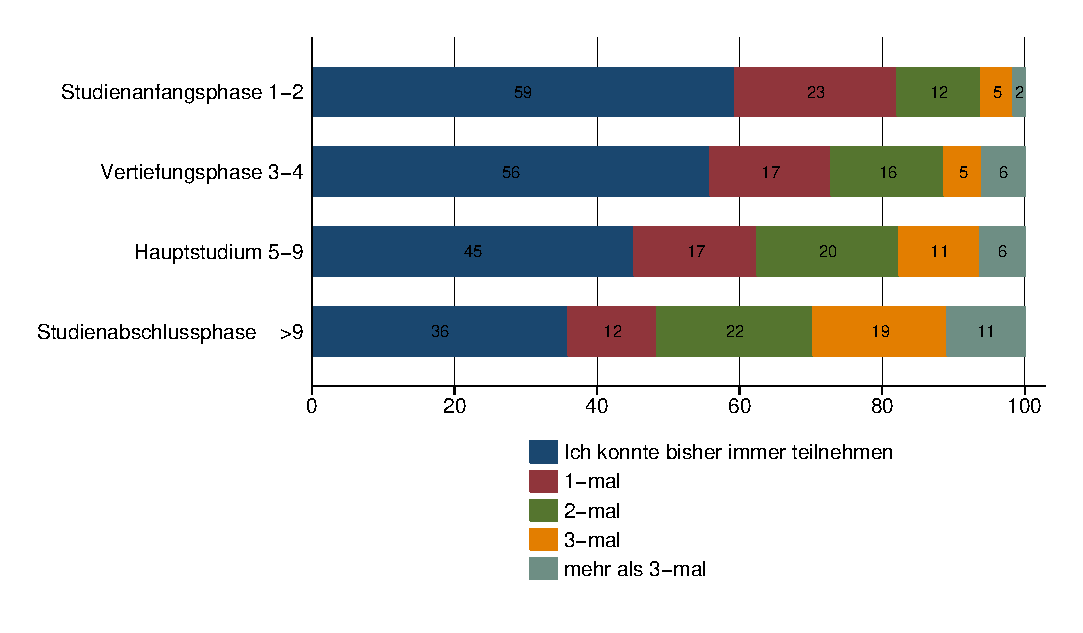
\includegraphics[RemoveGraphicsExtensions={.pdf,PDF}]{image}|
% \end{quote}
%
% \subsection{\plainTeX}
%
% \LaTeX's graphics packages can also be used with \plainTeX.
% The necessary basic \LaTeX\ macros are defined in
% \xfile{miniltx.tex}. This package \xpackage{grfext} also
% relies on it. Example:
%\begin{quote}
%\begin{verbatim}
%\input miniltx.tex\relax
%\def\Gin@driver{pdftex.def}
%\input graphicx.sty\relax
%\input grfext.sty\relax
%\resetatcatcode
%\end{verbatim}
%\end{quote}
%
% \StopEventually{
% }
%
% \section{Implementation}
%
%    \begin{macrocode}
%<*package>
%    \end{macrocode}
%
% \subsection{Relead check and identification}
%    Reload check, especially if the package is not used with \LaTeX.
%    \begin{macrocode}
\begingroup\catcode61\catcode48\catcode32=10\relax%
  \catcode13=5 % ^^M
  \endlinechar=13 %
  \catcode35=6 % #
  \catcode39=12 % '
  \catcode44=12 % ,
  \catcode45=12 % -
  \catcode46=12 % .
  \catcode58=12 % :
  \catcode64=11 % @
  \catcode123=1 % {
  \catcode125=2 % }
  \expandafter\let\expandafter\x\csname ver@grfext.sty\endcsname
  \ifx\x\relax % plain-TeX, first loading
  \else
    \def\empty{}%
    \ifx\x\empty % LaTeX, first loading,
      % variable is initialized, but \ProvidesPackage not yet seen
    \else
      \expandafter\ifx\csname PackageInfo\endcsname\relax
        \def\x#1#2{%
          \immediate\write-1{Package #1 Info: #2.}%
        }%
      \else
        \def\x#1#2{\PackageInfo{#1}{#2, stopped}}%
      \fi
      \x{grfext}{The package is already loaded}%
      \aftergroup\endinput
    \fi
  \fi
\endgroup%
%    \end{macrocode}
%    Package identification:
%    \begin{macrocode}
\begingroup\catcode61\catcode48\catcode32=10\relax%
  \catcode13=5 % ^^M
  \endlinechar=13 %
  \catcode35=6 % #
  \catcode39=12 % '
  \catcode40=12 % (
  \catcode41=12 % )
  \catcode44=12 % ,
  \catcode45=12 % -
  \catcode46=12 % .
  \catcode47=12 % /
  \catcode58=12 % :
  \catcode64=11 % @
  \catcode91=12 % [
  \catcode93=12 % ]
  \catcode123=1 % {
  \catcode125=2 % }
  \expandafter\ifx\csname ProvidesPackage\endcsname\relax
    \def\x#1#2#3[#4]{\endgroup
      \immediate\write-1{Package: #3 #4}%
      \xdef#1{#4}%
    }%
  \else
    \def\x#1#2[#3]{\endgroup
      #2[{#3}]%
      \ifx#1\@undefined
        \xdef#1{#3}%
      \fi
      \ifx#1\relax
        \xdef#1{#3}%
      \fi
    }%
  \fi
\expandafter\x\csname ver@grfext.sty\endcsname
\ProvidesPackage{grfext}%
  [2019/12/03 v1.3 Manage graphics extensions (HO)]%
%    \end{macrocode}
%
% \subsection{Catcodes}
%
%    \begin{macrocode}
\begingroup\catcode61\catcode48\catcode32=10\relax%
  \catcode13=5 % ^^M
  \endlinechar=13 %
  \catcode123=1 % {
  \catcode125=2 % }
  \catcode64=11 % @
  \def\x{\endgroup
    \expandafter\edef\csname grfext@AtEnd\endcsname{%
      \endlinechar=\the\endlinechar\relax
      \catcode13=\the\catcode13\relax
      \catcode32=\the\catcode32\relax
      \catcode35=\the\catcode35\relax
      \catcode61=\the\catcode61\relax
      \catcode64=\the\catcode64\relax
      \catcode123=\the\catcode123\relax
      \catcode125=\the\catcode125\relax
    }%
  }%
\x\catcode61\catcode48\catcode32=10\relax%
\catcode13=5 % ^^M
\endlinechar=13 %
\catcode35=6 % #
\catcode64=11 % @
\catcode123=1 % {
\catcode125=2 % }
\def\TMP@EnsureCode#1#2{%
  \edef\grfext@AtEnd{%
    \grfext@AtEnd
    \catcode#1=\the\catcode#1\relax
  }%
  \catcode#1=#2\relax
}
\TMP@EnsureCode{42}{12}% *
\TMP@EnsureCode{44}{12}% ,
\TMP@EnsureCode{47}{12}% /
\TMP@EnsureCode{58}{12}% :
\TMP@EnsureCode{60}{12}% <
\TMP@EnsureCode{62}{12}% >
\TMP@EnsureCode{91}{12}% [
\TMP@EnsureCode{93}{12}% ]
\edef\grfext@AtEnd{\grfext@AtEnd\noexpand\endinput}
%    \end{macrocode}
%
% \subsection{\plainTeX}
%
%    \begin{macro}{\@expandtwoargs}
%    Requirement is \xfile{miniltx.tex}, but we need also
%    \LaTeX's \cs{@expandtwoargs}.
%    \begin{macrocode}
\@ifundefined{@expandtwoargs}{%
  \def\@expandtwoargs#1#2#3{%
    \edef\reserved@a{\noexpand#1{#2}{#3}}%
    \reserved@a
  }%
}{}
%    \end{macrocode}
%    \end{macro}
%
% \subsection{Add}
%
%    \begin{macro}{\AppendGraphicsExtensions}
%    \begin{macrocode}
\newcommand*{\AppendGraphicsExtensions}{%
  \@ifundefined{Gin@extensions}{%
    \let\Gin@extensions\@empty
  }{}%
  \@ifstar{\grfext@Append\grfext@Check}{\grfext@Append\grfext@@Add}%
}%
%    \end{macrocode}
%    \end{macro}
%    \begin{macro}{\grfext@Append}
%    \begin{macrocode}
\def\grfext@Append#1#2{%
  \let\grfext@Print\@gobble
  \edef\grfext@next{%
    \noexpand\grfext@Add\noexpand#1{%
      \zap@space#2 \@empty
    }{\noexpand\Gin@extensions,}{}%
  }%
  \grfext@next
  \let\grfext@Print\grfext@@Print
  \grfext@Print\AppendGraphicsExtensions
}
%    \end{macrocode}
%    \end{macro}
%
%    \begin{macro}{\PrependGraphicsExtensions}
%    \begin{macrocode}
\newcommand*{\PrependGraphicsExtensions}{%
  \@ifundefined{Gin@extensions}{%
    \let\Gin@extensions\@empty
  }{}%
  \@ifstar{\grfext@Prepend\grfext@Check}{\grfext@Prepend\grfext@@Add}%
}%
%    \end{macrocode}
%    \end{macro}
%    \begin{macro}{\grfext@Prepend}
%    \begin{macrocode}
\def\grfext@Prepend#1#2{%
  \let\grfext@Print\@gobble
  \edef\grfext@next{%
    \noexpand\grfext@Add\noexpand#1{%
      \zap@space#2 \@empty
    }{}{,\noexpand\Gin@extensions}%
  }%
  \grfext@next
  \let\grfext@Print\grfext@@Print
  \grfext@Print\PrependGraphicsExtensions
}
%    \end{macrocode}
%    \end{macro}
%
%    \begin{macro}{\grfext@Add}
%    \begin{macrocode}
\def\grfext@Add#1#2{%
  #1{#2}%
}
%    \end{macrocode}
%    \end{macro}
%    \begin{macro}{\grfext@@Add}
%    \begin{macrocode}
\def\grfext@@Add#1#2#3{%
  \RemoveGraphicsExtensions{#1}%
  \ifx\Gin@extensions\@empty
    \def\Gin@extensions{#1}%
  \else
    \edef\Gin@extensions{#2#1#3}%
  \fi
}
%    \end{macrocode}
%    \end{macro}
%
% \subsection{Check}
%
%    \begin{macro}{\grfext@Check}
%    \begin{macrocode}
\def\grfext@Check#1{%
  \let\grfext@tmp\@empty
  \@for\grfext@ext:=#1\do{%
    \@ifundefined{Gin@rule@\grfext@ext}{%
    }{%
      \ifx\grfext@tmp\@empty
        \let\grfext@tmp\grfext@ext
      \else
        \edef\grfext@tmp{\grfext@tmp,\grfext@ext}%
      \fi
    }%
  }%
  \ifx\grfext@tmp\@empty
    \def\grfext@next##1##2{}%
  \else
    \edef\grfext@next{%
      \noexpand\grfext@@Add{\grfext@tmp}%
    }%
  \fi
  \grfext@next
}
%    \end{macrocode}
%    \end{macro}
%
% \subsection{Remove}
%
%    \begin{macro}{\RemoveGraphicsExtensions}
%    \begin{macrocode}
\newcommand*{\RemoveGraphicsExtensions}[1]{%
  \@ifundefined{Gin@extensions}{%
    \def\Gin@extensions{}%
  }{%
    \edef\grfext@tmp{\zap@space#1 \@empty}%
    \@for\grfext@ext:=\grfext@tmp\do{%
      \def\grfext@next{%
        \let\grfext@tmp\Gin@extensions
        \@expandtwoargs
        \@removeelement\grfext@ext\Gin@extensions\Gin@extensions
        \ifx\grfext@tmp\Gin@extensions
          \let\grfext@next\relax
        \fi
        \grfext@next
      }%
      \grfext@next
    }%
  }%
  \grfext@Print\RemoveGraphicsExtensions
}
%    \end{macrocode}
%    \end{macro}
%
% \subsection{Print}
%
%    \begin{macrocode}
\RequirePackage{infwarerr}[2007/09/09]
%    \end{macrocode}
%
%    \begin{macro}{\PrintGraphicsExtensions}
%    \begin{macrocode}
\def\PrintGraphicsExtensions{%
  \grfext@Print\PrintGraphicsExtensions
}
%    \end{macrocode}
%    \end{macro}
%    \begin{macro}{\grfext@Print}
%    \begin{macrocode}
\def\grfext@Print#1{%
  \@PackageInfo{grfext}{%
    Graphics extension search list:\MessageBreak
    \@ifundefined{Gin@extensions}{%
      <unavailable>%
    }{%
      [\Gin@extensions]%
    }\MessageBreak
    \string#1%
  }%
}
%    \end{macrocode}
%    \end{macro}
%    \begin{macro}{\grfext@@Print}
%    \begin{macrocode}
\let\grfext@@Print\grfext@Print
%    \end{macrocode}
%    \end{macro}
%
% \subsection{Defining options for package \xpackage{graphicx}}
%
%    \begin{macrocode}
\RequirePackage{kvdefinekeys}[2010/03/01]
\kv@define@key{Gin}{AppendGraphicsExtensions}{%
  \AppendGraphicsExtensions{#1}%
}
\kv@define@key{Gin}{AppendGraphicsExtensions*}{%
  \AppendGraphicsExtensions*{#1}%
}
\kv@define@key{Gin}{PrependGraphicsExtensions}{%
  \PrependGraphicsExtensions{#1}%
}
\kv@define@key{Gin}{PrependGraphicsExtensions*}{%
  \PrependGraphicsExtensions*{#1}%
}
\kv@define@key{Gin}{RemoveGraphicsExtensions}{%
  \RemoveGraphicsExtensions{#1}%
}
\kv@define@key{Gin}{PrintGraphicsExtensions}[]{%
  \PrintGraphicsExtensions
}
%    \end{macrocode}
%
%    \begin{macrocode}
\grfext@AtEnd%
%</package>
%    \end{macrocode}
% \section{Installation}
%
% \subsection{Download}
%
% \paragraph{Package.} This package is available on
% CTAN\footnote{\CTANpkg{grfext}}:
% \begin{description}
% \item[\CTAN{macros/latex/contrib/grfext/grfext.dtx}] The source file.
% \item[\CTAN{macros/latex/contrib/grfext/grfext.pdf}] Documentation.
% \end{description}
%
%
% \paragraph{Bundle.} All the packages of the bundle `grfext'
% are also available in a TDS compliant ZIP archive. There
% the packages are already unpacked and the documentation files
% are generated. The files and directories obey the TDS standard.
% \begin{description}
% \item[\CTANinstall{install/macros/latex/contrib/grfext.tds.zip}]
% \end{description}
% \emph{TDS} refers to the standard ``A Directory Structure
% for \TeX\ Files'' (\CTANpkg{tds}). Directories
% with \xfile{texmf} in their name are usually organized this way.
%
% \subsection{Bundle installation}
%
% \paragraph{Unpacking.} Unpack the \xfile{grfext.tds.zip} in the
% TDS tree (also known as \xfile{texmf} tree) of your choice.
% Example (linux):
% \begin{quote}
%   |unzip grfext.tds.zip -d ~/texmf|
% \end{quote}
%
% \subsection{Package installation}
%
% \paragraph{Unpacking.} The \xfile{.dtx} file is a self-extracting
% \docstrip\ archive. The files are extracted by running the
% \xfile{.dtx} through \plainTeX:
% \begin{quote}
%   \verb|tex grfext.dtx|
% \end{quote}
%
% \paragraph{TDS.} Now the different files must be moved into
% the different directories in your installation TDS tree
% (also known as \xfile{texmf} tree):
% \begin{quote}
% \def\t{^^A
% \begin{tabular}{@{}>{\ttfamily}l@{ $\rightarrow$ }>{\ttfamily}l@{}}
%   grfext.sty & tex/latex/grfext/grfext.sty\\
%   grfext.pdf & doc/latex/grfext/grfext.pdf\\
%   grfext.dtx & source/latex/grfext/grfext.dtx\\
% \end{tabular}^^A
% }^^A
% \sbox0{\t}^^A
% \ifdim\wd0>\linewidth
%   \begingroup
%     \advance\linewidth by\leftmargin
%     \advance\linewidth by\rightmargin
%   \edef\x{\endgroup
%     \def\noexpand\lw{\the\linewidth}^^A
%   }\x
%   \def\lwbox{^^A
%     \leavevmode
%     \hbox to \linewidth{^^A
%       \kern-\leftmargin\relax
%       \hss
%       \usebox0
%       \hss
%       \kern-\rightmargin\relax
%     }^^A
%   }^^A
%   \ifdim\wd0>\lw
%     \sbox0{\small\t}^^A
%     \ifdim\wd0>\linewidth
%       \ifdim\wd0>\lw
%         \sbox0{\footnotesize\t}^^A
%         \ifdim\wd0>\linewidth
%           \ifdim\wd0>\lw
%             \sbox0{\scriptsize\t}^^A
%             \ifdim\wd0>\linewidth
%               \ifdim\wd0>\lw
%                 \sbox0{\tiny\t}^^A
%                 \ifdim\wd0>\linewidth
%                   \lwbox
%                 \else
%                   \usebox0
%                 \fi
%               \else
%                 \lwbox
%               \fi
%             \else
%               \usebox0
%             \fi
%           \else
%             \lwbox
%           \fi
%         \else
%           \usebox0
%         \fi
%       \else
%         \lwbox
%       \fi
%     \else
%       \usebox0
%     \fi
%   \else
%     \lwbox
%   \fi
% \else
%   \usebox0
% \fi
% \end{quote}
% If you have a \xfile{docstrip.cfg} that configures and enables \docstrip's
% TDS installing feature, then some files can already be in the right
% place, see the documentation of \docstrip.
%
% \subsection{Refresh file name databases}
%
% If your \TeX~distribution
% (\TeX\,Live, \mikTeX, \dots) relies on file name databases, you must refresh
% these. For example, \TeX\,Live\ users run \verb|texhash| or
% \verb|mktexlsr|.
%
% \subsection{Some details for the interested}
%
% \paragraph{Unpacking with \LaTeX.}
% The \xfile{.dtx} chooses its action depending on the format:
% \begin{description}
% \item[\plainTeX:] Run \docstrip\ and extract the files.
% \item[\LaTeX:] Generate the documentation.
% \end{description}
% If you insist on using \LaTeX\ for \docstrip\ (really,
% \docstrip\ does not need \LaTeX), then inform the autodetect routine
% about your intention:
% \begin{quote}
%   \verb|latex \let\install=y\input{grfext.dtx}|
% \end{quote}
% Do not forget to quote the argument according to the demands
% of your shell.
%
% \paragraph{Generating the documentation.}
% You can use both the \xfile{.dtx} or the \xfile{.drv} to generate
% the documentation. The process can be configured by the
% configuration file \xfile{ltxdoc.cfg}. For instance, put this
% line into this file, if you want to have A4 as paper format:
% \begin{quote}
%   \verb|\PassOptionsToClass{a4paper}{article}|
% \end{quote}
% An example follows how to generate the
% documentation with pdf\LaTeX:
% \begin{quote}
%\begin{verbatim}
%pdflatex grfext.dtx
%makeindex -s gind.ist grfext.idx
%pdflatex grfext.dtx
%makeindex -s gind.ist grfext.idx
%pdflatex grfext.dtx
%\end{verbatim}
% \end{quote}
%
% \begin{thebibliography}{9}
%
% \bibitem{graphics}
%   David Carlisle, Sebastian Rahtz: \textit{The \xpackage{graphics} package};
%   2006/02/20 v1.0o;
%   \CTAN{macros/latex/required/graphics/graphics.dtx}.
%
% \end{thebibliography}
%
% \begin{History}
%   \begin{Version}{2007/09/30 v1.0}
%   \item
%     First public version.
%   \end{Version}
%   \begin{Version}{2010/08/19 v1.1}
%   \item
%     User macros are also made available as keyval options for
%     package \xpackage{graphicx}.
%   \end{Version}
%   \begin{Version}{2016/05/16 v1.2}
%   \item
%     Documentation updates.
%   \end{Version}
%   \begin{Version}{2019/12/03 v1.3}
%   \item
%     Documentation updates.
%   \end{Version}
% \end{History}
%
% \PrintIndex
%
% \Finale
\endinput
|
% \end{quote}
% Do not forget to quote the argument according to the demands
% of your shell.
%
% \paragraph{Generating the documentation.}
% You can use both the \xfile{.dtx} or the \xfile{.drv} to generate
% the documentation. The process can be configured by the
% configuration file \xfile{ltxdoc.cfg}. For instance, put this
% line into this file, if you want to have A4 as paper format:
% \begin{quote}
%   \verb|\PassOptionsToClass{a4paper}{article}|
% \end{quote}
% An example follows how to generate the
% documentation with pdf\LaTeX:
% \begin{quote}
%\begin{verbatim}
%pdflatex grfext.dtx
%makeindex -s gind.ist grfext.idx
%pdflatex grfext.dtx
%makeindex -s gind.ist grfext.idx
%pdflatex grfext.dtx
%\end{verbatim}
% \end{quote}
%
% \begin{thebibliography}{9}
%
% \bibitem{graphics}
%   David Carlisle, Sebastian Rahtz: \textit{The \xpackage{graphics} package};
%   2006/02/20 v1.0o;
%   \CTAN{macros/latex/required/graphics/graphics.dtx}.
%
% \end{thebibliography}
%
% \begin{History}
%   \begin{Version}{2007/09/30 v1.0}
%   \item
%     First public version.
%   \end{Version}
%   \begin{Version}{2010/08/19 v1.1}
%   \item
%     User macros are also made available as keyval options for
%     package \xpackage{graphicx}.
%   \end{Version}
%   \begin{Version}{2016/05/16 v1.2}
%   \item
%     Documentation updates.
%   \end{Version}
%   \begin{Version}{2019/12/03 v1.3}
%   \item
%     Documentation updates.
%   \end{Version}
% \end{History}
%
% \PrintIndex
%
% \Finale
\endinput
|
% \end{quote}
% Do not forget to quote the argument according to the demands
% of your shell.
%
% \paragraph{Generating the documentation.}
% You can use both the \xfile{.dtx} or the \xfile{.drv} to generate
% the documentation. The process can be configured by the
% configuration file \xfile{ltxdoc.cfg}. For instance, put this
% line into this file, if you want to have A4 as paper format:
% \begin{quote}
%   \verb|\PassOptionsToClass{a4paper}{article}|
% \end{quote}
% An example follows how to generate the
% documentation with pdf\LaTeX:
% \begin{quote}
%\begin{verbatim}
%pdflatex grfext.dtx
%makeindex -s gind.ist grfext.idx
%pdflatex grfext.dtx
%makeindex -s gind.ist grfext.idx
%pdflatex grfext.dtx
%\end{verbatim}
% \end{quote}
%
% \begin{thebibliography}{9}
%
% \bibitem{graphics}
%   David Carlisle, Sebastian Rahtz: \textit{The \xpackage{graphics} package};
%   2006/02/20 v1.0o;
%   \CTAN{macros/latex/required/graphics/graphics.dtx}.
%
% \end{thebibliography}
%
% \begin{History}
%   \begin{Version}{2007/09/30 v1.0}
%   \item
%     First public version.
%   \end{Version}
%   \begin{Version}{2010/08/19 v1.1}
%   \item
%     User macros are also made available as keyval options for
%     package \xpackage{graphicx}.
%   \end{Version}
%   \begin{Version}{2016/05/16 v1.2}
%   \item
%     Documentation updates.
%   \end{Version}
%   \begin{Version}{2019/12/03 v1.3}
%   \item
%     Documentation updates.
%   \end{Version}
% \end{History}
%
% \PrintIndex
%
% \Finale
\endinput
|
% \end{quote}
% Do not forget to quote the argument according to the demands
% of your shell.
%
% \paragraph{Generating the documentation.}
% You can use both the \xfile{.dtx} or the \xfile{.drv} to generate
% the documentation. The process can be configured by the
% configuration file \xfile{ltxdoc.cfg}. For instance, put this
% line into this file, if you want to have A4 as paper format:
% \begin{quote}
%   \verb|\PassOptionsToClass{a4paper}{article}|
% \end{quote}
% An example follows how to generate the
% documentation with pdf\LaTeX:
% \begin{quote}
%\begin{verbatim}
%pdflatex grfext.dtx
%makeindex -s gind.ist grfext.idx
%pdflatex grfext.dtx
%makeindex -s gind.ist grfext.idx
%pdflatex grfext.dtx
%\end{verbatim}
% \end{quote}
%
% \begin{thebibliography}{9}
%
% \bibitem{graphics}
%   David Carlisle, Sebastian Rahtz: \textit{The \xpackage{graphics} package};
%   2006/02/20 v1.0o;
%   \CTAN{macros/latex/required/graphics/graphics.dtx}.
%
% \end{thebibliography}
%
% \begin{History}
%   \begin{Version}{2007/09/30 v1.0}
%   \item
%     First public version.
%   \end{Version}
%   \begin{Version}{2010/08/19 v1.1}
%   \item
%     User macros are also made available as keyval options for
%     package \xpackage{graphicx}.
%   \end{Version}
%   \begin{Version}{2016/05/16 v1.2}
%   \item
%     Documentation updates.
%   \end{Version}
%   \begin{Version}{2019/12/03 v1.3}
%   \item
%     Documentation updates.
%   \end{Version}
% \end{History}
%
% \PrintIndex
%
% \Finale
\endinput
